%%%%%%%%%%%%%%%%%%%%%%%%%%%%%%%%%%%%%%%%%%%%%%%%%%%%%%%%%%%%%%%%%%%
%% analysis and results of the extended Lotka scheme
%% (C) Kenneth Geisshirt (kneth@chem.ruc.dk) 
%% Last modified: 30 January 1998
%%%%%%%%%%%%%%%%%%%%%%%%%%%%%%%%%%%%%%%%%%%%%%%%%%%%%%%%%%%%%%%%%%%

\chapter{The Extended Lotka Scheme}
\label{chap:ExtLotka}

Oscillating chemical reactions have intrigued chemists and many others
in the last 2--3 decades. The best known example is the reaction first
investigated by Belousov \cite{Belousov58} and Zhabotinsky
\cite{Zhabotinsky64}. One can only be fascinated by seeing the
solution in the reaction vessel changing colour every minute from deep
blue to red and back to blue again.

In this chapter we will look at simulations performed on a very simple
chemical mechanism, which is able to exhibit oscillations in the
concentrations as function of time. The mechanism is simulated by
Molecular Dynamics, and it is therefore a simulation with a finite
number of particles. It should be regarded as a prototype of an
oscillating chemical reaction.

The chapter is based upon the results described in two papers by the
author of the present thesis, Eigil L.\ Pr{\ae}stgaard, and
S{\o}ren Toxv{\ae}rd \cite{Geisshirt96a, Geisshirt97a} which are enclosed
as appendix \ref{app:B} and appendix \ref{app:C}


\section{A brief outline of previous studies}
The simulation of chemical reactions by Molecular Dynamics is not a
new approach. As early as 1975, Portnow \cite{Portnow75} simulated a
simple chemical reaction by Molecular Dynamics. Portnow studied the
fluctuations in the number density of the species \ie the
concentration. The simulated particles were hard spheres.

Ortoleva and coworkers \cite{Ortoleva76} were the first
to do MD simulations of chemical instabilities more than two decades
ago. The simulated mechanics was:

\begin{eqnarray*}
  X + Y &\rightarrow& 2X \\
  X     &\rightarrow& Y  \\
  Y     &\rightarrow& X
\end{eqnarray*}

The last two reactions are introduced in order to prevent that $Y$ is
converted to $X$. Ortoleva \etal imagined that the two reactions were
radiation processes so that the system can be far from equilibrium but
without a mass flux \ie the system is energetically driven. The
individual particles were hard spheres, and Ortoleva \etal simulated
up to 450 particles.  

Boissonade \cite{Boissonade79} studied almost two decades ago the
fluctuations in the concentration in two simple mechanisms
($A+C\rightarrow X+C, 2X\rightarrow 2N$ and $A+C \rightarrow X+C, 2X
\rightarrow X+N$). The system was two-dimensional and the particles
were hard disks. The simulation results are compared with a
master-equation approach.

In 1983 Heinrichs \etal \cite{Heinrichs83} performed simulations on
another oscillating reaction. The scheme was:

\begin{eqnarray*}
  A + B &\rightarrow& C     \\
  C + B &\rightarrow& D + B \\
  D     &\rightarrow& 2 B 
\end{eqnarray*}

In order to simulate an open system, Heinrichs \etal introduced an
inflow and an outflow of particles \ie the species $A$, $B$, $C$ and $D$
are created and removed randomly. Furthermore, there is an inert
species, $X$. If there are any inert species present in the system, an
$X$ particle is converted to one of the other species which mimics an
open system. If no inert species are present, a new particle is
created at a randomly chosen position. The first reaction creates an
inert particle, because the reaction really is $A+B \rightarrow
C+X$. In the third reaction a new particle (of type $B$) is
created. If the number of inert particles is larger than a certain
value, some of them are removed. All particles are hard spheres. It is
hard to tell exactly which ensemble Heinrichs \etal were simulating.

Recently, Diebner \etal \cite{Diebner95} simulated a very simple
mechanism. The mechanism is the same as we will present in section
\ref{sect:ExtLotkaMech}. The
particles interact through a long-ranged potential; basically a
repulsive Coulomb potential. The main result is that the mechanism is
oscillatory even on the microscopic level. In a very different
context, Frachebourg \etal \cite{Frachebourg96} have studied the same
mechanism as Diebner \textit{et al}.\footnote{Frachebourg \etal call the
  mechanism the cyclic Lotka-Volterra mechanism.} Moreover, Gorecki
\etal \cite{Gorecki97} have studied the same mechanism using hard
sphere Molecular Dynamics and a master equation. They conclude that the
spatial correlation functions oscillate in time, and that the
correlations are longer than for a stationary system.

Mansour \etal \cite{Mansour92} have recently written a very detailed
paper about the simulation of chemical reactions on a microscopic
level. The primary objective is to investigate complex mechanisms,
including oscillating reactions. The simulation technique is
\textit{not} Molecular Dynamics in the context of this thesis, but
is based upon Bird's algorithm \cite{Bird96} which is a numerical
solution of the Boltzmann equation. The particles considered by Mansour
\etal are hard spheres, and all reactions are binary.


To the best of our knowledge, only Toxv{\ae}rd \cite{Toxvaerd96a} has
considered reactions simulated by Molecular Dynamics in competition
with a phase transition (in that case, a spinodal decomposition). The
simulated system was a binary mixture of Lennard-Jones particles, and
the reaction scheme was $A \rightleftarrows B$. The result from these 
simulations is that chemical reactions have a strong influence on the
kinetics of the spinodal decomposition. In the last years an number of
papers has been published on which influence chemical reactions may
have on the phase separation process, see \eg Glotzer \etal
\cite{Glotzer94,Glotzer95}, Christensen \etal \cite{Christensen96}, and
Verdasca \etal \cite{Verdasca95}. The papers mainly investigate the
problem by modifying the Cahn-Hilliard equation to include chemical
reactions, and then solve it numerically. Recently, Carati \etal
\cite{Carati97} have contributed to the theoretical understanding by
analysing a such a Cahn-Hilliard based model. The work of Carati \etal
is mainly analytically, and their theoretical predictions have not been
be verified by \eg Molecular Dynamics simulations.


\section{The scheme}
\label{sect:ExtLotkaMech}
Lotka was one of the pioneers in the field of oscillating chemical
reactions. His work dates back to 1910s and 1920s, and his work was
purely theoretical - he himself was not convinced that oscillating
chemical reactions could occur in the real world. At the end of a paper
from 1910, Lotka wrote \cite{Lotka10}:

\begin{quotation}
\noindent No reaction is known to follow the above law [oscillatory],
and as a matter of fact the case here considered was suggested by the
consideration of matters lying outside the field of physical
chemistry.
\end{quotation}

His famous scheme from 1920 is \cite{Lotka20}:

\begin{subequations}
  \begin{eqnarray}
    A + X   &\rightarrow& 2X \\
    X + Y   &\rightarrow& 2Y \\
    Y       &\rightarrow& P
  \end{eqnarray}
\end{subequations}

The scheme above gives raise to oscillations in concentrations of $X$ and $Y$
when certain conditions are fulfilled. 

Lokta's scheme takes place in an open system; there is a constant
inflow of the species $A$ so that the concentration can be assumed to be
constant. Moreover, there is a constant outflow of the product
$P$.

Our scheme is very simple; it consists of three reactions and three
species only. We call it the extended Lotka scheme since it resembles
the Lotka scheme, and it is:


\begin{subequations}
  \begin{eqnarray}
    X + Y &\overset{k_1}{\rightarrow}& 2Y \label{Reac1} \\
    Y + Z &\overset{k_2}{\rightarrow}& 2Z \label{Reac2} \\
    Z + X &\overset{k_3}{\rightarrow}& 2X \label{Reac3}
  \end{eqnarray}
\end{subequations}
where $k_1$, $k_2$, and $k_3$ are the rate constants. We choose to let
the total concentration $[X]+[Y]+[Z]$ be constant and denoted $K$,
because we simulate a system where the total number of particles is
conserved. The scheme above violates the Wegschleider conditions
\cite{Diebner95}. This means that the extended Lotka scheme is
energetically driven, and the system will therefore always been far
from equilibrium.

From the reactions above, we are able to derive phenomenological
equations that describe the evolution of the concentrations. We
obtain three equations from the scheme given above:

\begin{subequations}
  \label{eq:PhenoODE}
  \begin{eqnarray}
    \diff{[X]}{t} &=& -k_1[X][Y] + k_3[X][Z] \label{eq:PhenoODEA} \\
    \diff{[Y]}{t} &=&  k_1[X][Y] - k_2[Y][Z] \label{eq:PhenoODEB} \\
    \diff{[Z]}{t} &=&  k_2[Y][Z] - k_3[X][Z] \label{eq:PhenoODEC}
  \end{eqnarray}
\end{subequations}

The differential equations above is an initial value problem, and given
the initial values of the concentrations of the three species, the
solution is unique. We have in principle three differential equations
but since the total concentration is constant, the solution will be in
a two-dimensional subspace of the three-dimensional concentration
space spanned by $[X]$, $[Y]$ and $[Z]$. A two-dimensional ordinary
differential equation cannot have chaotic solutions; this observation
is a consequence of the Poincar\'{e}-Bendixson theorem \cite[chapter
11]{Hirsch74}.

\section{Linear stability}
\label{sect:LinStabil}
The solution of the three phenomenological equations given in the
previous section will give us the evolution of concentrations of the
three species. But it is not possible to find an analytical solution. 

Instead of an analytical solution, we are able to obtain an
approximate solution. We will apply the technique of linear stability
of stationary points. The technique is introduced in section
\ref{sect:OscReacts}.

To begin, we find the stationary point \ie a point in the
concentration space where the differential is zero \ie we wish
to solve the set of equations:

\begin{subequations}
  \label{eq:StatPoint}
  \begin{eqnarray}
    \diff{[X]}{t} &=& -k_1[X][Y] + k_3[X][Z] = 0 \\
    \diff{[Y]}{t} &=&  k_1[X][Y] - k_2[Y][Z] = 0 \\
    \diff{[Z]}{t} &=&  k_2[Y][Z] - k_3[X][Z] = 0
  \end{eqnarray}
\end{subequations}

Let the stationary point be denoted $(x_{ss}, y_{ss}, z_{ss})$. At the
stationary point, the condition $K=x_{ss}+y_{ss}+z_{ss}$ must be
fulfilled. Solving equation \eqref{eq:StatPoint} we obtain

\begin{subequations}
  \label{eq:SteadyState}
  \begin{eqnarray}
    x_{ss} &=& \frac{Kk_2}{k_1+k_2+k_3} \\
    y_{ss} &=& \frac{Kk_3}{k_1+k_2+k_3} \\
    z_{ss} &=& \frac{Kk_1}{k_1+k_2+k_3}
  \end{eqnarray}
\end{subequations}

Close to the stationary point, we can linearise the ordinary
differential equations and solve the linear equations. The
approximative solution close to the stationary point is then 

\begin{equation}
  \left(\begin{array}{c}\, [X]\\ \, [Y]\\ \, [Z]\end{array}\right)
  =   \left(\begin{array}{c} x_{ss}\\ y_{ss}\\ z_{ss}\end{array}\right)
   + \sum_i \vec{e}_i e^{\lambda_i t}
\end{equation}
where $\vec{e}_i$ is the $i$th eigenvector (scaled appropriately) and
$\lambda_i$ is the $i$th eigenvalue of the Jacobian matrix. We are
only interested to see whether the extended Lotka scheme is
oscillatory, so we only calculate the eigenvalues. The extended Lotka
scheme has one zero eigenvalue and two complex conjugated which are

\begin{equation}
  \lambda = \pm \frac{K\sqrt{k_1+k_2+k_3}}{\sqrt{k_1k_2k_3}} \imath
\end{equation}

We conclude that the stationary state is stable, and the
motion (close to the stationary state) is a harmonic oscillation.

\section{Molecular details}
\label{sect:MolecDetail}
The extended Lotka mechanism as analysed in the previous sections, can
be simulated by Molecular Dynamics. In this section we discuss the
molecular details. 

The three species, $X$, $Y$ and $Z$, are chosen to be atoms. The
interaction potential is the Lennard-Jones potential \ie

\begin{equation}
\label{eq:LJpot}
  u_{\smbox{LJ}}(r) = 4\epsilon \left[\left(\frac{\sigma}{r}\right)^{12} -
    \left(\frac{\sigma}{r}\right)^6 \right]
\end{equation}
where $\epsilon$ is the minimum of the potential (and the fundamental
energy unit), and $\sigma$ is the characteristic length. The minimum
of the potential is easily\footnote{Differentiate
  \protect$u_{\smbox{LJ}}(r)\protect$ with respect to
  \protect$r\protect$, set it equal to zero and solve with respect to
  \protect$r\protect$.} found to be $\sqrt[6]{2}\sigma$. 

We have simulated two different systems. They are:

\begin{description}
\item[System 1] All the particles are identical \ie the difference is
  only the ``colour'' of the particles. The ``colour'' represent the
  species \ie in our case there are three ``colours''. The potential
  is $u_{\smbox{I}}(r) = u_{\smbox{LJ}}(r)$.
\item[System 2] The particles of the same ``colour'' interact through
  the Lennard-Jones potential given by equation
  \eqref{eq:LJpot}. Particles of different ``colours'' \eg the $X$-$Y$
  interaction, is non-attractive. In order to simulate this, we use
  the following potential

  \begin{equation}
    u_{\smbox{II}}(r) = 
    \begin{cases}
      u_{\smbox{LJ}}(r) &\text{for $r\le \sqrt[6]{2}\sigma$} \\
      0                 &\text{otherwise}
    \end{cases}
  \end{equation}
\end{description}

A system like System 2 is known to phase separate below a certain
critical temperature \cite{Laradji96,Toxvaerd95a}.

As mentioned in section \ref{sect:SimulChemReact}, the simulation of
chemical reactions requires two parameters for a binary reaction. The
first parameter is the sum of radii of two colliding particles,
$R_{\smbox{reac}}$. In most cases we set $R_{\smbox{reac}}=0.96116\sigma$
which ensures that only particles with a large relative velocity might
be counted as colliding particles. The algorithms presented in chapter
\ref{chap:NumTech} are applied, and the temperature is controlled by the
Nos\'{e}-Hoover thermostat.


\section{Steady and oscillatory states in the microscopic system}
In section \ref{sect:LinStabil} we found the stationary state for the
extended Lotka scheme. A stationary state is a state where the
concentrations are constant. If the phenomenological equations
\eqref{eq:PhenoODE} represent the microscopic details of the system,
the steady state given by equation \eqref{eq:SteadyState} must be
reproducible by the MD simulations. 

Consider a system where $k_1=k_2=k_3$. The steady state is then
$x_s=y_s=z_s = \frac{K}{3}$. We set up a simulation with $1/3$ of
the particles of each species. Figure \ref{fig:steady} shows the
result. From the figure it is obvious that a steady state exists for
the finite system. The fluctuations in the concentration (measured by
the particle fraction) decrease with the number of particles.

\begin{figure}
  \begin{center}
%\epsfig{file=Lotka/steady.ps,width=7.5cm,height=7.5cm}
    % GNUPLOT: LaTeX picture
\setlength{\unitlength}{0.240900pt}
\ifx\plotpoint\undefined\newsavebox{\plotpoint}\fi
\sbox{\plotpoint}{\rule[-0.200pt]{0.400pt}{0.400pt}}%
\begin{picture}(1500,900)(0,0)
\font\gnuplot=cmr10 at 10pt
\gnuplot
\sbox{\plotpoint}{\rule[-0.200pt]{0.400pt}{0.400pt}}%
\put(201.0,163.0){\rule[-0.200pt]{4.818pt}{0.400pt}}
\put(181,163){\makebox(0,0)[r]{0.3}}
\put(1460.0,163.0){\rule[-0.200pt]{4.818pt}{0.400pt}}
\put(201.0,302.0){\rule[-0.200pt]{4.818pt}{0.400pt}}
\put(181,302){\makebox(0,0)[r]{0.32}}
\put(1460.0,302.0){\rule[-0.200pt]{4.818pt}{0.400pt}}
\put(201.0,441.0){\rule[-0.200pt]{4.818pt}{0.400pt}}
\put(181,441){\makebox(0,0)[r]{0.34}}
\put(1460.0,441.0){\rule[-0.200pt]{4.818pt}{0.400pt}}
\put(201.0,581.0){\rule[-0.200pt]{4.818pt}{0.400pt}}
\put(181,581){\makebox(0,0)[r]{0.36}}
\put(1460.0,581.0){\rule[-0.200pt]{4.818pt}{0.400pt}}
\put(201.0,720.0){\rule[-0.200pt]{4.818pt}{0.400pt}}
\put(181,720){\makebox(0,0)[r]{0.38}}
\put(1460.0,720.0){\rule[-0.200pt]{4.818pt}{0.400pt}}
\put(201.0,859.0){\rule[-0.200pt]{4.818pt}{0.400pt}}
\put(181,859){\makebox(0,0)[r]{0.4}}
\put(1460.0,859.0){\rule[-0.200pt]{4.818pt}{0.400pt}}
\put(201.0,163.0){\rule[-0.200pt]{0.400pt}{4.818pt}}
\put(201,122){\makebox(0,0){0}}
\put(201.0,839.0){\rule[-0.200pt]{0.400pt}{4.818pt}}
\put(286.0,163.0){\rule[-0.200pt]{0.400pt}{4.818pt}}
\put(286,122){\makebox(0,0){10}}
\put(286.0,839.0){\rule[-0.200pt]{0.400pt}{4.818pt}}
\put(371.0,163.0){\rule[-0.200pt]{0.400pt}{4.818pt}}
\put(371,122){\makebox(0,0){20}}
\put(371.0,839.0){\rule[-0.200pt]{0.400pt}{4.818pt}}
\put(457.0,163.0){\rule[-0.200pt]{0.400pt}{4.818pt}}
\put(457,122){\makebox(0,0){30}}
\put(457.0,839.0){\rule[-0.200pt]{0.400pt}{4.818pt}}
\put(542.0,163.0){\rule[-0.200pt]{0.400pt}{4.818pt}}
\put(542,122){\makebox(0,0){40}}
\put(542.0,839.0){\rule[-0.200pt]{0.400pt}{4.818pt}}
\put(627.0,163.0){\rule[-0.200pt]{0.400pt}{4.818pt}}
\put(627,122){\makebox(0,0){50}}
\put(627.0,839.0){\rule[-0.200pt]{0.400pt}{4.818pt}}
\put(713.0,163.0){\rule[-0.200pt]{0.400pt}{4.818pt}}
\put(713,122){\makebox(0,0){60}}
\put(713.0,839.0){\rule[-0.200pt]{0.400pt}{4.818pt}}
\put(798.0,163.0){\rule[-0.200pt]{0.400pt}{4.818pt}}
\put(798,122){\makebox(0,0){70}}
\put(798.0,839.0){\rule[-0.200pt]{0.400pt}{4.818pt}}
\put(883.0,163.0){\rule[-0.200pt]{0.400pt}{4.818pt}}
\put(883,122){\makebox(0,0){80}}
\put(883.0,839.0){\rule[-0.200pt]{0.400pt}{4.818pt}}
\put(968.0,163.0){\rule[-0.200pt]{0.400pt}{4.818pt}}
\put(968,122){\makebox(0,0){90}}
\put(968.0,839.0){\rule[-0.200pt]{0.400pt}{4.818pt}}
\put(1054.0,163.0){\rule[-0.200pt]{0.400pt}{4.818pt}}
\put(1054,122){\makebox(0,0){100}}
\put(1054.0,839.0){\rule[-0.200pt]{0.400pt}{4.818pt}}
\put(1139.0,163.0){\rule[-0.200pt]{0.400pt}{4.818pt}}
\put(1139,122){\makebox(0,0){110}}
\put(1139.0,839.0){\rule[-0.200pt]{0.400pt}{4.818pt}}
\put(1224.0,163.0){\rule[-0.200pt]{0.400pt}{4.818pt}}
\put(1224,122){\makebox(0,0){120}}
\put(1224.0,839.0){\rule[-0.200pt]{0.400pt}{4.818pt}}
\put(1309.0,163.0){\rule[-0.200pt]{0.400pt}{4.818pt}}
\put(1309,122){\makebox(0,0){130}}
\put(1309.0,839.0){\rule[-0.200pt]{0.400pt}{4.818pt}}
\put(1395.0,163.0){\rule[-0.200pt]{0.400pt}{4.818pt}}
\put(1395,122){\makebox(0,0){140}}
\put(1395.0,839.0){\rule[-0.200pt]{0.400pt}{4.818pt}}
\put(1480.0,163.0){\rule[-0.200pt]{0.400pt}{4.818pt}}
\put(1480,122){\makebox(0,0){150}}
\put(1480.0,839.0){\rule[-0.200pt]{0.400pt}{4.818pt}}
\put(201.0,163.0){\rule[-0.200pt]{308.111pt}{0.400pt}}
\put(1480.0,163.0){\rule[-0.200pt]{0.400pt}{167.666pt}}
\put(201.0,859.0){\rule[-0.200pt]{308.111pt}{0.400pt}}
\put(41,511){\makebox(0,0){$x_X$}}
\put(840,61){\makebox(0,0){time}}
\put(201.0,163.0){\rule[-0.200pt]{0.400pt}{167.666pt}}
\put(201,393){\usebox{\plotpoint}}
\put(201,393){\usebox{\plotpoint}}
\put(201,393){\usebox{\plotpoint}}
\put(201,393){\usebox{\plotpoint}}
\put(201,393){\usebox{\plotpoint}}
\put(201,393){\usebox{\plotpoint}}
\put(201,393){\usebox{\plotpoint}}
\put(201,393){\usebox{\plotpoint}}
\put(201,393){\usebox{\plotpoint}}
\put(201,393){\usebox{\plotpoint}}
\put(201,393){\usebox{\plotpoint}}
\put(201,393){\usebox{\plotpoint}}
\put(201.0,393.0){\usebox{\plotpoint}}
\put(202.0,386.0){\rule[-0.200pt]{0.400pt}{1.686pt}}
\put(202.0,386.0){\usebox{\plotpoint}}
\put(203.0,379.0){\rule[-0.200pt]{0.400pt}{1.686pt}}
\put(203.0,379.0){\usebox{\plotpoint}}
\put(204.0,379.0){\rule[-0.200pt]{0.400pt}{1.686pt}}
\put(204.0,372.0){\rule[-0.200pt]{0.400pt}{3.373pt}}
\put(204.0,372.0){\usebox{\plotpoint}}
\put(205.0,372.0){\rule[-0.200pt]{0.400pt}{1.686pt}}
\put(205.0,379.0){\rule[-0.200pt]{0.482pt}{0.400pt}}
\put(207.0,379.0){\rule[-0.200pt]{0.400pt}{1.686pt}}
\put(207.0,379.0){\rule[-0.200pt]{0.400pt}{1.686pt}}
\put(207.0,379.0){\usebox{\plotpoint}}
\put(208.0,372.0){\rule[-0.200pt]{0.400pt}{1.686pt}}
\put(208.0,372.0){\rule[-0.200pt]{0.723pt}{0.400pt}}
\put(211.0,372.0){\rule[-0.200pt]{0.400pt}{1.686pt}}
\put(211.0,366.0){\rule[-0.200pt]{0.400pt}{3.132pt}}
\put(211.0,366.0){\usebox{\plotpoint}}
\put(212.0,366.0){\rule[-0.200pt]{0.400pt}{1.445pt}}
\put(212.0,366.0){\rule[-0.200pt]{0.400pt}{1.445pt}}
\put(212.0,366.0){\rule[-0.200pt]{0.723pt}{0.400pt}}
\put(215.0,366.0){\rule[-0.200pt]{0.400pt}{1.445pt}}
\put(215.0,366.0){\rule[-0.200pt]{0.400pt}{1.445pt}}
\put(215.0,366.0){\usebox{\plotpoint}}
\put(216.0,359.0){\rule[-0.200pt]{0.400pt}{1.686pt}}
\put(216.0,359.0){\usebox{\plotpoint}}
\put(217.0,359.0){\rule[-0.200pt]{0.400pt}{1.686pt}}
\put(217.0,366.0){\rule[-0.200pt]{0.482pt}{0.400pt}}
\put(219.0,359.0){\rule[-0.200pt]{0.400pt}{1.686pt}}
\put(219.0,359.0){\usebox{\plotpoint}}
\put(219.67,366){\rule{0.400pt}{1.445pt}}
\multiput(219.17,366.00)(1.000,3.000){2}{\rule{0.400pt}{0.723pt}}
\put(220.0,359.0){\rule[-0.200pt]{0.400pt}{1.686pt}}
\put(221,372){\usebox{\plotpoint}}
\put(221,372){\usebox{\plotpoint}}
\put(221,372){\usebox{\plotpoint}}
\put(221,372){\usebox{\plotpoint}}
\put(221,372){\usebox{\plotpoint}}
\put(221,372){\usebox{\plotpoint}}
\put(221,372){\usebox{\plotpoint}}
\put(221.0,366.0){\rule[-0.200pt]{0.400pt}{1.445pt}}
\put(221.0,366.0){\rule[-0.200pt]{1.204pt}{0.400pt}}
\put(226.0,366.0){\rule[-0.200pt]{0.400pt}{1.445pt}}
\put(226.0,372.0){\rule[-0.200pt]{0.482pt}{0.400pt}}
\put(228.0,366.0){\rule[-0.200pt]{0.400pt}{1.445pt}}
\put(228.0,366.0){\rule[-0.200pt]{0.400pt}{1.445pt}}
\put(228.0,372.0){\usebox{\plotpoint}}
\put(229.0,366.0){\rule[-0.200pt]{0.400pt}{1.445pt}}
\put(229.0,366.0){\usebox{\plotpoint}}
\put(230.0,352.0){\rule[-0.200pt]{0.400pt}{3.373pt}}
\put(230.0,352.0){\rule[-0.200pt]{0.400pt}{1.686pt}}
\put(230.0,359.0){\usebox{\plotpoint}}
\put(231.0,359.0){\rule[-0.200pt]{0.400pt}{1.686pt}}
\put(231.0,366.0){\rule[-0.200pt]{0.482pt}{0.400pt}}
\put(233.0,352.0){\rule[-0.200pt]{0.400pt}{3.373pt}}
\put(233.0,352.0){\usebox{\plotpoint}}
\put(234.0,352.0){\rule[-0.200pt]{0.400pt}{1.686pt}}
\put(234.0,359.0){\usebox{\plotpoint}}
\put(235.0,359.0){\rule[-0.200pt]{0.400pt}{1.686pt}}
\put(235.0,366.0){\usebox{\plotpoint}}
\put(236.0,366.0){\rule[-0.200pt]{0.400pt}{1.445pt}}
\put(236.0,366.0){\rule[-0.200pt]{0.400pt}{1.445pt}}
\put(236.0,366.0){\usebox{\plotpoint}}
\put(237.0,359.0){\rule[-0.200pt]{0.400pt}{1.686pt}}
\put(237.0,359.0){\rule[-0.200pt]{0.964pt}{0.400pt}}
\put(241.0,359.0){\rule[-0.200pt]{0.400pt}{1.686pt}}
\put(241.0,366.0){\usebox{\plotpoint}}
\put(242.0,366.0){\rule[-0.200pt]{0.400pt}{3.132pt}}
\put(242.0,379.0){\usebox{\plotpoint}}
\put(243.0,379.0){\rule[-0.200pt]{0.400pt}{1.686pt}}
\put(243.0,386.0){\rule[-0.200pt]{0.482pt}{0.400pt}}
\put(244.67,393){\rule{0.400pt}{1.686pt}}
\multiput(244.17,393.00)(1.000,3.500){2}{\rule{0.400pt}{0.843pt}}
\put(245.0,386.0){\rule[-0.200pt]{0.400pt}{1.686pt}}
\put(246,400){\usebox{\plotpoint}}
\put(246,400){\usebox{\plotpoint}}
\put(246,400){\usebox{\plotpoint}}
\put(246,400){\usebox{\plotpoint}}
\put(246,400){\usebox{\plotpoint}}
\put(246,400){\usebox{\plotpoint}}
\put(246.0,400.0){\rule[-0.200pt]{0.400pt}{3.132pt}}
\put(246.0,406.0){\rule[-0.200pt]{0.400pt}{1.686pt}}
\put(246.0,406.0){\usebox{\plotpoint}}
\put(247.0,406.0){\rule[-0.200pt]{0.400pt}{1.686pt}}
\put(247.0,406.0){\rule[-0.200pt]{0.400pt}{1.686pt}}
\put(247.0,406.0){\usebox{\plotpoint}}
\put(248.0,400.0){\rule[-0.200pt]{0.400pt}{1.445pt}}
\put(248.0,400.0){\usebox{\plotpoint}}
\put(249.0,393.0){\rule[-0.200pt]{0.400pt}{1.686pt}}
\put(249.0,393.0){\usebox{\plotpoint}}
\put(250.0,393.0){\rule[-0.200pt]{0.400pt}{1.686pt}}
\put(250.0,393.0){\rule[-0.200pt]{0.400pt}{1.686pt}}
\put(250.0,393.0){\rule[-0.200pt]{0.482pt}{0.400pt}}
\put(252.0,393.0){\rule[-0.200pt]{0.400pt}{3.132pt}}
\put(252.0,406.0){\rule[-0.200pt]{0.723pt}{0.400pt}}
\put(255.0,406.0){\rule[-0.200pt]{0.400pt}{1.686pt}}
\put(255.0,413.0){\usebox{\plotpoint}}
\put(256.0,406.0){\rule[-0.200pt]{0.400pt}{1.686pt}}
\put(256.0,406.0){\rule[-0.200pt]{1.445pt}{0.400pt}}
\put(262.0,400.0){\rule[-0.200pt]{0.400pt}{1.445pt}}
\put(262.0,400.0){\rule[-0.200pt]{0.400pt}{1.445pt}}
\put(262.0,406.0){\rule[-0.200pt]{0.482pt}{0.400pt}}
\put(264.0,400.0){\rule[-0.200pt]{0.400pt}{1.445pt}}
\put(264.0,400.0){\usebox{\plotpoint}}
\put(265.0,400.0){\rule[-0.200pt]{0.400pt}{1.445pt}}
\put(265.0,393.0){\rule[-0.200pt]{0.400pt}{3.132pt}}
\put(265.0,393.0){\rule[-0.200pt]{0.400pt}{1.686pt}}
\put(265.0,400.0){\usebox{\plotpoint}}
\put(266.0,400.0){\rule[-0.200pt]{0.400pt}{1.445pt}}
\put(266.0,406.0){\usebox{\plotpoint}}
\put(267.0,400.0){\rule[-0.200pt]{0.400pt}{1.445pt}}
\put(267.0,400.0){\rule[-0.200pt]{0.400pt}{3.132pt}}
\put(267.0,413.0){\usebox{\plotpoint}}
\put(268.0,406.0){\rule[-0.200pt]{0.400pt}{1.686pt}}
\put(268.0,406.0){\rule[-0.200pt]{0.400pt}{1.686pt}}
\put(268.0,406.0){\rule[-0.200pt]{0.400pt}{1.686pt}}
\put(268.0,406.0){\usebox{\plotpoint}}
\put(269.0,406.0){\rule[-0.200pt]{0.400pt}{1.686pt}}
\put(269.0,400.0){\rule[-0.200pt]{0.400pt}{3.132pt}}
\put(269.0,400.0){\rule[-0.200pt]{0.964pt}{0.400pt}}
\put(273.0,386.0){\rule[-0.200pt]{0.400pt}{3.373pt}}
\put(273.0,386.0){\rule[-0.200pt]{0.723pt}{0.400pt}}
\put(276.0,386.0){\rule[-0.200pt]{0.400pt}{1.686pt}}
\put(276.0,393.0){\rule[-0.200pt]{0.723pt}{0.400pt}}
\put(279.0,379.0){\rule[-0.200pt]{0.400pt}{3.373pt}}
\put(279.0,379.0){\rule[-0.200pt]{0.482pt}{0.400pt}}
\put(281.0,372.0){\rule[-0.200pt]{0.400pt}{1.686pt}}
\put(281.0,372.0){\rule[-0.200pt]{0.723pt}{0.400pt}}
\put(284.0,372.0){\rule[-0.200pt]{0.400pt}{1.686pt}}
\put(284.0,379.0){\rule[-0.200pt]{0.482pt}{0.400pt}}
\put(286.0,352.0){\rule[-0.200pt]{0.400pt}{6.504pt}}
\put(286.0,352.0){\rule[-0.200pt]{0.482pt}{0.400pt}}
\put(288.0,352.0){\rule[-0.200pt]{0.400pt}{1.686pt}}
\put(288.0,359.0){\rule[-0.200pt]{0.482pt}{0.400pt}}
\put(290.0,359.0){\rule[-0.200pt]{0.400pt}{3.132pt}}
\put(290.0,372.0){\usebox{\plotpoint}}
\put(291.0,366.0){\rule[-0.200pt]{0.400pt}{1.445pt}}
\put(291.0,366.0){\usebox{\plotpoint}}
\put(292.0,359.0){\rule[-0.200pt]{0.400pt}{1.686pt}}
\put(292.0,359.0){\usebox{\plotpoint}}
\put(293.0,352.0){\rule[-0.200pt]{0.400pt}{1.686pt}}
\put(293.0,352.0){\rule[-0.200pt]{0.723pt}{0.400pt}}
\put(296.0,352.0){\rule[-0.200pt]{0.400pt}{1.686pt}}
\put(296.0,359.0){\usebox{\plotpoint}}
\put(297.0,359.0){\rule[-0.200pt]{0.400pt}{3.132pt}}
\put(297.0,372.0){\rule[-0.200pt]{0.723pt}{0.400pt}}
\put(300.0,372.0){\rule[-0.200pt]{0.400pt}{1.686pt}}
\put(300.0,379.0){\usebox{\plotpoint}}
\put(301.0,372.0){\rule[-0.200pt]{0.400pt}{1.686pt}}
\put(301.0,372.0){\rule[-0.200pt]{0.723pt}{0.400pt}}
\put(304.0,372.0){\rule[-0.200pt]{0.400pt}{1.686pt}}
\put(304.0,372.0){\rule[-0.200pt]{0.400pt}{1.686pt}}
\put(304.0,372.0){\rule[-0.200pt]{0.400pt}{1.686pt}}
\put(304.0,379.0){\rule[-0.200pt]{0.482pt}{0.400pt}}
\put(306.0,379.0){\rule[-0.200pt]{0.400pt}{1.686pt}}
\put(306.0,386.0){\rule[-0.200pt]{0.723pt}{0.400pt}}
\put(309.0,386.0){\rule[-0.200pt]{0.400pt}{1.686pt}}
\put(309.0,393.0){\rule[-0.200pt]{0.482pt}{0.400pt}}
\put(311.0,393.0){\rule[-0.200pt]{0.400pt}{1.686pt}}
\put(311.0,400.0){\usebox{\plotpoint}}
\put(312.0,400.0){\rule[-0.200pt]{0.400pt}{3.132pt}}
\put(312.0,413.0){\rule[-0.200pt]{0.482pt}{0.400pt}}
\put(314.0,413.0){\rule[-0.200pt]{0.400pt}{1.686pt}}
\put(314.0,413.0){\rule[-0.200pt]{0.400pt}{1.686pt}}
\put(314.0,413.0){\rule[-0.200pt]{0.400pt}{3.373pt}}
\put(314.0,427.0){\rule[-0.200pt]{0.482pt}{0.400pt}}
\put(316.0,420.0){\rule[-0.200pt]{0.400pt}{1.686pt}}
\put(316.0,420.0){\rule[-0.200pt]{0.400pt}{1.686pt}}
\put(316.0,427.0){\usebox{\plotpoint}}
\put(317.0,420.0){\rule[-0.200pt]{0.400pt}{1.686pt}}
\put(317.0,420.0){\usebox{\plotpoint}}
\put(318.0,413.0){\rule[-0.200pt]{0.400pt}{1.686pt}}
\put(318.0,413.0){\rule[-0.200pt]{0.482pt}{0.400pt}}
\put(320.0,406.0){\rule[-0.200pt]{0.400pt}{1.686pt}}
\put(320.0,406.0){\rule[-0.200pt]{0.964pt}{0.400pt}}
\put(324.0,406.0){\rule[-0.200pt]{0.400pt}{1.686pt}}
\put(324.0,406.0){\rule[-0.200pt]{0.400pt}{1.686pt}}
\put(324.0,406.0){\usebox{\plotpoint}}
\put(325.0,400.0){\rule[-0.200pt]{0.400pt}{1.445pt}}
\put(325.0,400.0){\usebox{\plotpoint}}
\put(326.0,386.0){\rule[-0.200pt]{0.400pt}{3.373pt}}
\put(326.0,386.0){\rule[-0.200pt]{0.482pt}{0.400pt}}
\put(328.0,379.0){\rule[-0.200pt]{0.400pt}{1.686pt}}
\put(328.0,379.0){\usebox{\plotpoint}}
\put(329.0,372.0){\rule[-0.200pt]{0.400pt}{1.686pt}}
\put(329.0,372.0){\usebox{\plotpoint}}
\put(330.0,366.0){\rule[-0.200pt]{0.400pt}{1.445pt}}
\put(330.0,366.0){\usebox{\plotpoint}}
\put(331.0,366.0){\rule[-0.200pt]{0.400pt}{3.132pt}}
\put(331.0,372.0){\rule[-0.200pt]{0.400pt}{1.686pt}}
\put(331.0,372.0){\rule[-0.200pt]{0.400pt}{1.686pt}}
\put(331.0,379.0){\rule[-0.200pt]{0.964pt}{0.400pt}}
\put(335.0,379.0){\rule[-0.200pt]{0.400pt}{1.686pt}}
\put(335.0,386.0){\rule[-0.200pt]{0.482pt}{0.400pt}}
\put(337.0,379.0){\rule[-0.200pt]{0.400pt}{1.686pt}}
\put(337.0,379.0){\usebox{\plotpoint}}
\put(338.0,379.0){\rule[-0.200pt]{0.400pt}{1.686pt}}
\put(338.0,386.0){\rule[-0.200pt]{0.723pt}{0.400pt}}
\put(341.0,386.0){\rule[-0.200pt]{0.400pt}{1.686pt}}
\put(341.0,393.0){\rule[-0.200pt]{0.723pt}{0.400pt}}
\put(344.0,386.0){\rule[-0.200pt]{0.400pt}{1.686pt}}
\put(344.0,386.0){\usebox{\plotpoint}}
\put(345.0,386.0){\rule[-0.200pt]{0.400pt}{1.686pt}}
\put(345.0,393.0){\rule[-0.200pt]{0.482pt}{0.400pt}}
\put(347.0,386.0){\rule[-0.200pt]{0.400pt}{1.686pt}}
\put(347.0,386.0){\rule[-0.200pt]{0.400pt}{1.686pt}}
\put(347.0,393.0){\rule[-0.200pt]{1.204pt}{0.400pt}}
\put(352.0,393.0){\rule[-0.200pt]{0.400pt}{1.686pt}}
\put(352.0,393.0){\rule[-0.200pt]{0.400pt}{1.686pt}}
\put(352.0,393.0){\usebox{\plotpoint}}
\put(353.0,393.0){\rule[-0.200pt]{0.400pt}{1.686pt}}
\put(353.0,400.0){\rule[-0.200pt]{0.482pt}{0.400pt}}
\put(355.0,393.0){\rule[-0.200pt]{0.400pt}{1.686pt}}
\put(354.67,400){\rule{0.400pt}{1.445pt}}
\multiput(354.17,400.00)(1.000,3.000){2}{\rule{0.400pt}{0.723pt}}
\put(355.0,393.0){\rule[-0.200pt]{0.400pt}{1.686pt}}
\put(356,406){\usebox{\plotpoint}}
\put(356,406){\usebox{\plotpoint}}
\put(356,406){\usebox{\plotpoint}}
\put(356,406){\usebox{\plotpoint}}
\put(356,406){\usebox{\plotpoint}}
\put(356,406){\usebox{\plotpoint}}
\put(356,406){\usebox{\plotpoint}}
\put(356,406){\usebox{\plotpoint}}
\put(356,406){\usebox{\plotpoint}}
\put(356,406){\usebox{\plotpoint}}
\put(356,406){\usebox{\plotpoint}}
\put(356,406){\usebox{\plotpoint}}
\put(356,406){\usebox{\plotpoint}}
\put(356,406){\usebox{\plotpoint}}
\put(356,406){\usebox{\plotpoint}}
\put(356,406){\usebox{\plotpoint}}
\put(356,406){\usebox{\plotpoint}}
\put(356,406){\usebox{\plotpoint}}
\put(356,406){\usebox{\plotpoint}}
\put(356,406){\usebox{\plotpoint}}
\put(356,406){\usebox{\plotpoint}}
\put(356,406){\usebox{\plotpoint}}
\put(356,406){\usebox{\plotpoint}}
\put(356.0,406.0){\rule[-0.200pt]{0.482pt}{0.400pt}}
\put(358.0,406.0){\rule[-0.200pt]{0.400pt}{1.686pt}}
\put(358.0,406.0){\rule[-0.200pt]{0.400pt}{1.686pt}}
\put(358.0,406.0){\usebox{\plotpoint}}
\put(359.0,400.0){\rule[-0.200pt]{0.400pt}{1.445pt}}
\put(359.0,400.0){\usebox{\plotpoint}}
\put(360.0,400.0){\rule[-0.200pt]{0.400pt}{1.445pt}}
\put(360.0,406.0){\rule[-0.200pt]{0.482pt}{0.400pt}}
\put(362.0,406.0){\rule[-0.200pt]{0.400pt}{1.686pt}}
\put(362.0,413.0){\usebox{\plotpoint}}
\put(363.0,406.0){\rule[-0.200pt]{0.400pt}{1.686pt}}
\put(363.0,406.0){\usebox{\plotpoint}}
\put(364.0,393.0){\rule[-0.200pt]{0.400pt}{3.132pt}}
\put(364.0,393.0){\usebox{\plotpoint}}
\put(365.0,393.0){\rule[-0.200pt]{0.400pt}{3.132pt}}
\put(365.0,406.0){\usebox{\plotpoint}}
\put(366.0,406.0){\rule[-0.200pt]{0.400pt}{1.686pt}}
\put(366.0,413.0){\usebox{\plotpoint}}
\put(367.0,413.0){\rule[-0.200pt]{0.400pt}{1.686pt}}
\put(367.0,420.0){\usebox{\plotpoint}}
\put(367.67,434){\rule{0.400pt}{1.445pt}}
\multiput(367.17,434.00)(1.000,3.000){2}{\rule{0.400pt}{0.723pt}}
\put(368.0,420.0){\rule[-0.200pt]{0.400pt}{3.373pt}}
\put(369,440){\usebox{\plotpoint}}
\put(369,440){\usebox{\plotpoint}}
\put(369,440){\usebox{\plotpoint}}
\put(369,440){\usebox{\plotpoint}}
\put(369,440){\usebox{\plotpoint}}
\put(369,440){\usebox{\plotpoint}}
\put(369,440){\usebox{\plotpoint}}
\put(369,440){\usebox{\plotpoint}}
\put(369.0,440.0){\rule[-0.200pt]{0.400pt}{1.686pt}}
\put(369.0,447.0){\usebox{\plotpoint}}
\put(370.0,440.0){\rule[-0.200pt]{0.400pt}{1.686pt}}
\put(370.0,440.0){\usebox{\plotpoint}}
\put(371.0,434.0){\rule[-0.200pt]{0.400pt}{1.445pt}}
\put(371.0,434.0){\rule[-0.200pt]{0.482pt}{0.400pt}}
\put(373.0,427.0){\rule[-0.200pt]{0.400pt}{1.686pt}}
\put(373.0,427.0){\rule[-0.200pt]{0.482pt}{0.400pt}}
\put(375.0,427.0){\rule[-0.200pt]{0.400pt}{1.686pt}}
\put(375.0,434.0){\usebox{\plotpoint}}
\put(376.0,413.0){\rule[-0.200pt]{0.400pt}{5.059pt}}
\put(376.0,413.0){\usebox{\plotpoint}}
\put(377.0,406.0){\rule[-0.200pt]{0.400pt}{1.686pt}}
\put(377.0,406.0){\rule[-0.200pt]{0.723pt}{0.400pt}}
\put(380.0,406.0){\rule[-0.200pt]{0.400pt}{1.686pt}}
\put(380.0,413.0){\rule[-0.200pt]{0.723pt}{0.400pt}}
\put(383.0,413.0){\rule[-0.200pt]{0.400pt}{1.686pt}}
\put(383.0,420.0){\rule[-0.200pt]{0.964pt}{0.400pt}}
\put(387.0,420.0){\rule[-0.200pt]{0.400pt}{3.373pt}}
\put(387.0,434.0){\rule[-0.200pt]{0.723pt}{0.400pt}}
\put(390.0,427.0){\rule[-0.200pt]{0.400pt}{1.686pt}}
\put(390.0,427.0){\rule[-0.200pt]{0.400pt}{1.686pt}}
\put(390.0,434.0){\rule[-0.200pt]{1.686pt}{0.400pt}}
\put(397.0,427.0){\rule[-0.200pt]{0.400pt}{1.686pt}}
\put(397.67,427){\rule{0.400pt}{1.686pt}}
\multiput(397.17,427.00)(1.000,3.500){2}{\rule{0.400pt}{0.843pt}}
\put(397.0,427.0){\usebox{\plotpoint}}
\put(399,434){\usebox{\plotpoint}}
\put(399,434){\usebox{\plotpoint}}
\put(399,434){\usebox{\plotpoint}}
\put(399,434){\usebox{\plotpoint}}
\put(399,434){\usebox{\plotpoint}}
\put(399,434){\usebox{\plotpoint}}
\put(399.0,434.0){\rule[-0.200pt]{0.400pt}{1.445pt}}
\put(399.0,440.0){\rule[-0.200pt]{0.723pt}{0.400pt}}
\put(402.0,434.0){\rule[-0.200pt]{0.400pt}{1.445pt}}
\put(402.0,434.0){\rule[-0.200pt]{0.482pt}{0.400pt}}
\put(404.0,434.0){\rule[-0.200pt]{0.400pt}{3.132pt}}
\put(404.0,447.0){\usebox{\plotpoint}}
\put(405.0,440.0){\rule[-0.200pt]{0.400pt}{1.686pt}}
\put(405.0,440.0){\usebox{\plotpoint}}
\put(406.0,434.0){\rule[-0.200pt]{0.400pt}{1.445pt}}
\put(406.0,434.0){\rule[-0.200pt]{0.400pt}{1.445pt}}
\put(406.0,440.0){\rule[-0.200pt]{0.482pt}{0.400pt}}
\put(408.0,440.0){\rule[-0.200pt]{0.400pt}{1.686pt}}
\put(408.0,447.0){\rule[-0.200pt]{0.482pt}{0.400pt}}
\put(410.0,447.0){\rule[-0.200pt]{0.400pt}{1.686pt}}
\put(411.67,447){\rule{0.400pt}{1.686pt}}
\multiput(411.17,450.50)(1.000,-3.500){2}{\rule{0.400pt}{0.843pt}}
\put(410.0,454.0){\rule[-0.200pt]{0.482pt}{0.400pt}}
\put(413,447){\usebox{\plotpoint}}
\put(413,447){\usebox{\plotpoint}}
\put(413,447){\usebox{\plotpoint}}
\put(413,447){\usebox{\plotpoint}}
\put(413,447){\usebox{\plotpoint}}
\put(413,447){\usebox{\plotpoint}}
\put(413,447){\usebox{\plotpoint}}
\put(413,447){\usebox{\plotpoint}}
\put(413,447){\usebox{\plotpoint}}
\put(413,447){\usebox{\plotpoint}}
\put(413,447){\usebox{\plotpoint}}
\put(413,447){\usebox{\plotpoint}}
\put(413,447){\usebox{\plotpoint}}
\put(413,447){\usebox{\plotpoint}}
\put(413,447){\usebox{\plotpoint}}
\put(413,447){\usebox{\plotpoint}}
\put(413,447){\usebox{\plotpoint}}
\put(413,447){\usebox{\plotpoint}}
\put(413,447){\usebox{\plotpoint}}
\put(413,447){\usebox{\plotpoint}}
\put(413,447){\usebox{\plotpoint}}
\put(413,447){\usebox{\plotpoint}}
\put(413.0,447.0){\rule[-0.200pt]{0.400pt}{1.686pt}}
\put(413.0,454.0){\rule[-0.200pt]{0.723pt}{0.400pt}}
\put(416.0,447.0){\rule[-0.200pt]{0.400pt}{1.686pt}}
\put(416.0,447.0){\rule[-0.200pt]{0.482pt}{0.400pt}}
\put(417.67,440){\rule{0.400pt}{1.686pt}}
\multiput(417.17,440.00)(1.000,3.500){2}{\rule{0.400pt}{0.843pt}}
\put(418.0,440.0){\rule[-0.200pt]{0.400pt}{1.686pt}}
\put(419.0,447.0){\rule[-0.200pt]{0.400pt}{1.686pt}}
\put(419.0,454.0){\rule[-0.200pt]{0.723pt}{0.400pt}}
\put(422.0,454.0){\rule[-0.200pt]{0.400pt}{1.686pt}}
\put(422.0,461.0){\usebox{\plotpoint}}
\put(423.0,461.0){\rule[-0.200pt]{0.400pt}{3.132pt}}
\put(423.0,474.0){\rule[-0.200pt]{0.482pt}{0.400pt}}
\put(425.0,474.0){\rule[-0.200pt]{0.400pt}{1.686pt}}
\put(425.0,481.0){\usebox{\plotpoint}}
\put(426.0,467.0){\rule[-0.200pt]{0.400pt}{3.373pt}}
\put(426.0,467.0){\rule[-0.200pt]{0.723pt}{0.400pt}}
\put(429.0,461.0){\rule[-0.200pt]{0.400pt}{1.445pt}}
\put(429.0,461.0){\usebox{\plotpoint}}
\put(430.0,461.0){\rule[-0.200pt]{0.400pt}{1.445pt}}
\put(430.0,467.0){\usebox{\plotpoint}}
\put(431.0,461.0){\rule[-0.200pt]{0.400pt}{1.445pt}}
\put(431.0,461.0){\usebox{\plotpoint}}
\put(432.0,461.0){\rule[-0.200pt]{0.400pt}{3.132pt}}
\put(431.67,467){\rule{0.400pt}{1.686pt}}
\multiput(431.17,467.00)(1.000,3.500){2}{\rule{0.400pt}{0.843pt}}
\put(432.0,467.0){\rule[-0.200pt]{0.400pt}{1.686pt}}
\put(433,474){\usebox{\plotpoint}}
\put(433,474){\usebox{\plotpoint}}
\put(433,474){\usebox{\plotpoint}}
\put(433,474){\usebox{\plotpoint}}
\put(433,474){\usebox{\plotpoint}}
\put(433,474){\usebox{\plotpoint}}
\put(433,474){\usebox{\plotpoint}}
\put(433,474){\usebox{\plotpoint}}
\put(433,474){\usebox{\plotpoint}}
\put(433,474){\usebox{\plotpoint}}
\put(433,474){\usebox{\plotpoint}}
\put(433,474){\usebox{\plotpoint}}
\put(433,474){\usebox{\plotpoint}}
\put(433,474){\usebox{\plotpoint}}
\put(433,474){\usebox{\plotpoint}}
\put(433,474){\usebox{\plotpoint}}
\put(433,474){\usebox{\plotpoint}}
\put(433,474){\usebox{\plotpoint}}
\put(433.0,474.0){\rule[-0.200pt]{0.400pt}{3.373pt}}
\put(433.0,488.0){\rule[-0.200pt]{0.482pt}{0.400pt}}
\put(435.0,474.0){\rule[-0.200pt]{0.400pt}{3.373pt}}
\put(435.0,474.0){\usebox{\plotpoint}}
\put(436.0,474.0){\rule[-0.200pt]{0.400pt}{1.686pt}}
\put(436.0,481.0){\usebox{\plotpoint}}
\put(437.0,474.0){\rule[-0.200pt]{0.400pt}{1.686pt}}
\put(437.0,474.0){\usebox{\plotpoint}}
\put(438.0,474.0){\rule[-0.200pt]{0.400pt}{1.686pt}}
\put(438.0,481.0){\usebox{\plotpoint}}
\put(439.0,461.0){\rule[-0.200pt]{0.400pt}{4.818pt}}
\put(439.0,461.0){\rule[-0.200pt]{0.964pt}{0.400pt}}
\put(443.0,461.0){\rule[-0.200pt]{0.400pt}{1.445pt}}
\put(443.0,467.0){\rule[-0.200pt]{0.482pt}{0.400pt}}
\put(445.0,467.0){\rule[-0.200pt]{0.400pt}{1.686pt}}
\put(445.0,474.0){\rule[-0.200pt]{0.723pt}{0.400pt}}
\put(448.0,474.0){\rule[-0.200pt]{0.400pt}{1.686pt}}
\put(448.0,481.0){\usebox{\plotpoint}}
\put(449.0,481.0){\rule[-0.200pt]{0.400pt}{1.686pt}}
\put(449.0,481.0){\rule[-0.200pt]{0.400pt}{1.686pt}}
\put(449.0,481.0){\usebox{\plotpoint}}
\put(450.0,481.0){\rule[-0.200pt]{0.400pt}{1.686pt}}
\put(450.0,488.0){\usebox{\plotpoint}}
\put(450.67,495){\rule{0.400pt}{1.445pt}}
\multiput(450.17,498.00)(1.000,-3.000){2}{\rule{0.400pt}{0.723pt}}
\put(451.0,488.0){\rule[-0.200pt]{0.400pt}{3.132pt}}
\put(452,495){\usebox{\plotpoint}}
\put(452,495){\usebox{\plotpoint}}
\put(452.0,488.0){\rule[-0.200pt]{0.400pt}{1.686pt}}
\put(452.0,488.0){\rule[-0.200pt]{0.482pt}{0.400pt}}
\put(454.0,488.0){\rule[-0.200pt]{0.400pt}{1.686pt}}
\put(454.0,488.0){\rule[-0.200pt]{0.400pt}{1.686pt}}
\put(454.0,488.0){\usebox{\plotpoint}}
\put(455.0,488.0){\rule[-0.200pt]{0.400pt}{1.686pt}}
\put(455.0,495.0){\usebox{\plotpoint}}
\put(456.0,488.0){\rule[-0.200pt]{0.400pt}{1.686pt}}
\put(456.0,488.0){\rule[-0.200pt]{0.400pt}{1.686pt}}
\put(456.0,495.0){\usebox{\plotpoint}}
\put(457.0,495.0){\rule[-0.200pt]{0.400pt}{1.445pt}}
\put(457.0,501.0){\usebox{\plotpoint}}
\put(458.0,495.0){\rule[-0.200pt]{0.400pt}{1.445pt}}
\put(458.0,495.0){\rule[-0.200pt]{0.400pt}{1.445pt}}
\put(458.0,501.0){\rule[-0.200pt]{0.482pt}{0.400pt}}
\put(460.0,501.0){\rule[-0.200pt]{0.400pt}{3.373pt}}
\put(460.0,515.0){\usebox{\plotpoint}}
\put(461.0,515.0){\rule[-0.200pt]{0.400pt}{1.686pt}}
\put(461.0,522.0){\rule[-0.200pt]{0.482pt}{0.400pt}}
\put(463.0,515.0){\rule[-0.200pt]{0.400pt}{1.686pt}}
\put(463.0,515.0){\rule[-0.200pt]{0.482pt}{0.400pt}}
\put(465.0,501.0){\rule[-0.200pt]{0.400pt}{3.373pt}}
\put(465.0,501.0){\usebox{\plotpoint}}
\put(466.0,501.0){\rule[-0.200pt]{0.400pt}{1.686pt}}
\put(466.0,501.0){\rule[-0.200pt]{0.400pt}{1.686pt}}
\put(466.0,501.0){\rule[-0.200pt]{0.400pt}{3.373pt}}
\put(466.0,515.0){\rule[-0.200pt]{0.964pt}{0.400pt}}
\put(470.0,508.0){\rule[-0.200pt]{0.400pt}{1.686pt}}
\put(470.0,508.0){\rule[-0.200pt]{0.400pt}{1.686pt}}
\put(470.0,515.0){\usebox{\plotpoint}}
\put(471.0,508.0){\rule[-0.200pt]{0.400pt}{1.686pt}}
\put(471.0,508.0){\rule[-0.200pt]{0.400pt}{1.686pt}}
\put(471.0,515.0){\usebox{\plotpoint}}
\put(472.0,508.0){\rule[-0.200pt]{0.400pt}{1.686pt}}
\put(472.0,508.0){\rule[-0.200pt]{0.400pt}{1.686pt}}
\put(472.0,508.0){\rule[-0.200pt]{0.400pt}{1.686pt}}
\put(472.0,508.0){\usebox{\plotpoint}}
\put(473.0,508.0){\rule[-0.200pt]{0.400pt}{1.686pt}}
\put(473.0,508.0){\rule[-0.200pt]{0.400pt}{1.686pt}}
\put(473.0,508.0){\usebox{\plotpoint}}
\put(474.0,508.0){\rule[-0.200pt]{0.400pt}{1.686pt}}
\put(474.0,515.0){\usebox{\plotpoint}}
\put(475.0,515.0){\rule[-0.200pt]{0.400pt}{1.686pt}}
\put(475.0,522.0){\usebox{\plotpoint}}
\put(476.0,522.0){\rule[-0.200pt]{0.400pt}{1.686pt}}
\put(476.0,529.0){\rule[-0.200pt]{0.482pt}{0.400pt}}
\put(478.0,522.0){\rule[-0.200pt]{0.400pt}{1.686pt}}
\put(478.0,522.0){\rule[-0.200pt]{0.400pt}{3.132pt}}
\put(478.0,535.0){\rule[-0.200pt]{0.482pt}{0.400pt}}
\put(480.0,535.0){\rule[-0.200pt]{0.400pt}{1.686pt}}
\put(480.0,542.0){\usebox{\plotpoint}}
\put(481.0,529.0){\rule[-0.200pt]{0.400pt}{3.132pt}}
\put(481.0,529.0){\usebox{\plotpoint}}
\put(482.0,529.0){\rule[-0.200pt]{0.400pt}{4.818pt}}
\put(482.0,549.0){\usebox{\plotpoint}}
\put(483.0,542.0){\rule[-0.200pt]{0.400pt}{1.686pt}}
\put(483.0,542.0){\rule[-0.200pt]{0.400pt}{1.686pt}}
\put(483.0,549.0){\rule[-0.200pt]{0.723pt}{0.400pt}}
\put(486.0,549.0){\rule[-0.200pt]{0.400pt}{4.818pt}}
\put(486.0,569.0){\rule[-0.200pt]{0.482pt}{0.400pt}}
\put(488.0,556.0){\rule[-0.200pt]{0.400pt}{3.132pt}}
\put(488.0,556.0){\usebox{\plotpoint}}
\put(489.0,556.0){\rule[-0.200pt]{0.400pt}{1.686pt}}
\put(489.0,563.0){\rule[-0.200pt]{0.723pt}{0.400pt}}
\put(492.0,535.0){\rule[-0.200pt]{0.400pt}{6.745pt}}
\put(492.0,535.0){\usebox{\plotpoint}}
\put(493.0,535.0){\rule[-0.200pt]{0.400pt}{1.686pt}}
\put(493.0,542.0){\rule[-0.200pt]{0.482pt}{0.400pt}}
\put(495.0,542.0){\rule[-0.200pt]{0.400pt}{1.686pt}}
\put(495.0,549.0){\rule[-0.200pt]{1.686pt}{0.400pt}}
\put(502.0,549.0){\rule[-0.200pt]{0.400pt}{1.686pt}}
\put(502.0,556.0){\usebox{\plotpoint}}
\put(503.0,556.0){\rule[-0.200pt]{0.400pt}{3.132pt}}
\put(503.0,569.0){\rule[-0.200pt]{0.482pt}{0.400pt}}
\put(505.0,569.0){\rule[-0.200pt]{0.400pt}{3.373pt}}
\put(505.0,583.0){\usebox{\plotpoint}}
\put(506.0,583.0){\rule[-0.200pt]{0.400pt}{1.686pt}}
\put(506.0,590.0){\usebox{\plotpoint}}
\put(507.0,583.0){\rule[-0.200pt]{0.400pt}{1.686pt}}
\put(507.0,583.0){\rule[-0.200pt]{0.400pt}{1.686pt}}
\put(507.0,590.0){\rule[-0.200pt]{0.482pt}{0.400pt}}
\put(509.0,590.0){\rule[-0.200pt]{0.400pt}{1.686pt}}
\put(509.0,597.0){\usebox{\plotpoint}}
\put(510.0,597.0){\rule[-0.200pt]{0.400pt}{1.445pt}}
\put(510.0,603.0){\rule[-0.200pt]{0.482pt}{0.400pt}}
\put(512.0,603.0){\rule[-0.200pt]{0.400pt}{1.686pt}}
\put(512.0,610.0){\rule[-0.200pt]{0.723pt}{0.400pt}}
\put(515.0,603.0){\rule[-0.200pt]{0.400pt}{1.686pt}}
\put(515.0,603.0){\rule[-0.200pt]{0.482pt}{0.400pt}}
\put(517.0,597.0){\rule[-0.200pt]{0.400pt}{1.445pt}}
\put(517.0,597.0){\rule[-0.200pt]{0.482pt}{0.400pt}}
\put(519.0,597.0){\rule[-0.200pt]{0.400pt}{1.445pt}}
\put(519.0,603.0){\rule[-0.200pt]{1.204pt}{0.400pt}}
\put(524.0,590.0){\rule[-0.200pt]{0.400pt}{3.132pt}}
\put(524.0,590.0){\usebox{\plotpoint}}
\put(524.67,583){\rule{0.400pt}{1.686pt}}
\multiput(524.17,583.00)(1.000,3.500){2}{\rule{0.400pt}{0.843pt}}
\put(525.0,583.0){\rule[-0.200pt]{0.400pt}{1.686pt}}
\put(526,590){\usebox{\plotpoint}}
\put(526,590){\usebox{\plotpoint}}
\put(526,590){\usebox{\plotpoint}}
\put(526,590){\usebox{\plotpoint}}
\put(526,590){\usebox{\plotpoint}}
\put(526,590){\usebox{\plotpoint}}
\put(526,590){\usebox{\plotpoint}}
\put(526,590){\usebox{\plotpoint}}
\put(526,590){\usebox{\plotpoint}}
\put(526,590){\usebox{\plotpoint}}
\put(526,590){\usebox{\plotpoint}}
\put(526,590){\usebox{\plotpoint}}
\put(526,590){\usebox{\plotpoint}}
\put(526,590){\usebox{\plotpoint}}
\put(526,590){\usebox{\plotpoint}}
\put(526,590){\usebox{\plotpoint}}
\put(526,590){\usebox{\plotpoint}}
\put(526,590){\usebox{\plotpoint}}
\put(526,590){\usebox{\plotpoint}}
\put(526,590){\usebox{\plotpoint}}
\put(526,590){\usebox{\plotpoint}}
\put(526,590){\usebox{\plotpoint}}
\put(526.0,590.0){\rule[-0.200pt]{0.723pt}{0.400pt}}
\put(529.0,583.0){\rule[-0.200pt]{0.400pt}{1.686pt}}
\put(529.0,583.0){\usebox{\plotpoint}}
\put(530.0,569.0){\rule[-0.200pt]{0.400pt}{3.373pt}}
\put(530.0,569.0){\usebox{\plotpoint}}
\put(531.0,563.0){\rule[-0.200pt]{0.400pt}{1.445pt}}
\put(531.0,563.0){\usebox{\plotpoint}}
\put(532.0,563.0){\rule[-0.200pt]{0.400pt}{1.445pt}}
\put(532.0,569.0){\rule[-0.200pt]{0.723pt}{0.400pt}}
\put(535.0,569.0){\rule[-0.200pt]{0.400pt}{3.373pt}}
\put(535.0,583.0){\rule[-0.200pt]{0.964pt}{0.400pt}}
\put(539.0,583.0){\rule[-0.200pt]{0.400pt}{3.373pt}}
\put(539.0,597.0){\rule[-0.200pt]{0.482pt}{0.400pt}}
\put(541.0,590.0){\rule[-0.200pt]{0.400pt}{1.686pt}}
\put(541.0,590.0){\rule[-0.200pt]{0.482pt}{0.400pt}}
\put(543.0,590.0){\rule[-0.200pt]{0.400pt}{1.686pt}}
\put(543.0,597.0){\rule[-0.200pt]{0.482pt}{0.400pt}}
\put(545.0,597.0){\rule[-0.200pt]{0.400pt}{1.445pt}}
\put(545.0,603.0){\usebox{\plotpoint}}
\put(546.0,603.0){\rule[-0.200pt]{0.400pt}{1.686pt}}
\put(546.0,610.0){\rule[-0.200pt]{0.482pt}{0.400pt}}
\put(548.0,610.0){\rule[-0.200pt]{0.400pt}{1.686pt}}
\put(548.0,617.0){\usebox{\plotpoint}}
\put(549.0,617.0){\rule[-0.200pt]{0.400pt}{3.373pt}}
\put(549.0,631.0){\usebox{\plotpoint}}
\put(550.0,617.0){\rule[-0.200pt]{0.400pt}{3.373pt}}
\put(550.0,617.0){\rule[-0.200pt]{0.482pt}{0.400pt}}
\put(552.0,617.0){\rule[-0.200pt]{0.400pt}{1.686pt}}
\put(552.0,624.0){\usebox{\plotpoint}}
\put(553.0,624.0){\rule[-0.200pt]{0.400pt}{3.132pt}}
\put(553.0,637.0){\usebox{\plotpoint}}
\put(554.0,637.0){\rule[-0.200pt]{0.400pt}{1.686pt}}
\put(554.0,644.0){\usebox{\plotpoint}}
\put(555.0,637.0){\rule[-0.200pt]{0.400pt}{1.686pt}}
\put(555.0,637.0){\usebox{\plotpoint}}
\put(556.0,637.0){\rule[-0.200pt]{0.400pt}{1.686pt}}
\put(556.0,644.0){\usebox{\plotpoint}}
\put(557.0,624.0){\rule[-0.200pt]{0.400pt}{4.818pt}}
\put(557.0,624.0){\usebox{\plotpoint}}
\put(558.0,624.0){\rule[-0.200pt]{0.400pt}{1.686pt}}
\put(558.0,631.0){\rule[-0.200pt]{0.482pt}{0.400pt}}
\put(560.0,624.0){\rule[-0.200pt]{0.400pt}{1.686pt}}
\put(560.0,624.0){\rule[-0.200pt]{0.482pt}{0.400pt}}
\put(562.0,624.0){\rule[-0.200pt]{0.400pt}{1.686pt}}
\put(562.0,631.0){\usebox{\plotpoint}}
\put(563.0,631.0){\rule[-0.200pt]{0.400pt}{4.818pt}}
\put(563.0,651.0){\rule[-0.200pt]{0.482pt}{0.400pt}}
\put(565.0,651.0){\rule[-0.200pt]{0.400pt}{1.686pt}}
\put(565.0,658.0){\usebox{\plotpoint}}
\put(566.0,658.0){\rule[-0.200pt]{0.400pt}{1.686pt}}
\put(566.0,665.0){\usebox{\plotpoint}}
\put(567.0,665.0){\rule[-0.200pt]{0.400pt}{1.445pt}}
\put(567.0,671.0){\rule[-0.200pt]{0.482pt}{0.400pt}}
\put(569.0,665.0){\rule[-0.200pt]{0.400pt}{1.445pt}}
\put(569.0,665.0){\rule[-0.200pt]{0.723pt}{0.400pt}}
\put(572.0,665.0){\rule[-0.200pt]{0.400pt}{1.445pt}}
\put(572.0,671.0){\usebox{\plotpoint}}
\put(573.0,665.0){\rule[-0.200pt]{0.400pt}{1.445pt}}
\put(573.0,665.0){\rule[-0.200pt]{0.400pt}{1.445pt}}
\put(573.0,671.0){\rule[-0.200pt]{1.686pt}{0.400pt}}
\put(580.0,671.0){\rule[-0.200pt]{0.400pt}{3.373pt}}
\put(580.0,685.0){\rule[-0.200pt]{0.482pt}{0.400pt}}
\put(582.0,685.0){\rule[-0.200pt]{0.400pt}{1.686pt}}
\put(582.0,685.0){\rule[-0.200pt]{0.400pt}{1.686pt}}
\put(582.0,685.0){\rule[-0.200pt]{0.723pt}{0.400pt}}
\put(585.0,678.0){\rule[-0.200pt]{0.400pt}{1.686pt}}
\put(587.67,671){\rule{0.400pt}{1.686pt}}
\multiput(587.17,674.50)(1.000,-3.500){2}{\rule{0.400pt}{0.843pt}}
\put(585.0,678.0){\rule[-0.200pt]{0.723pt}{0.400pt}}
\put(589,671){\usebox{\plotpoint}}
\put(589.0,665.0){\rule[-0.200pt]{0.400pt}{1.445pt}}
\put(589.0,665.0){\rule[-0.200pt]{0.400pt}{1.445pt}}
\put(589.0,671.0){\usebox{\plotpoint}}
\put(589.67,665){\rule{0.400pt}{1.445pt}}
\multiput(589.17,665.00)(1.000,3.000){2}{\rule{0.400pt}{0.723pt}}
\put(590.0,665.0){\rule[-0.200pt]{0.400pt}{1.445pt}}
\put(591,671){\usebox{\plotpoint}}
\put(591,671){\usebox{\plotpoint}}
\put(591,671){\usebox{\plotpoint}}
\put(591,671){\usebox{\plotpoint}}
\put(591,671){\usebox{\plotpoint}}
\put(591,671){\usebox{\plotpoint}}
\put(591,671){\usebox{\plotpoint}}
\put(591,671){\usebox{\plotpoint}}
\put(591,671){\usebox{\plotpoint}}
\put(591,671){\usebox{\plotpoint}}
\put(591,671){\usebox{\plotpoint}}
\put(591,671){\usebox{\plotpoint}}
\put(591,671){\usebox{\plotpoint}}
\put(591,671){\usebox{\plotpoint}}
\put(591,671){\usebox{\plotpoint}}
\put(591,671){\usebox{\plotpoint}}
\put(591,671){\usebox{\plotpoint}}
\put(591,671){\usebox{\plotpoint}}
\put(591,671){\usebox{\plotpoint}}
\put(591,671){\usebox{\plotpoint}}
\put(591,671){\usebox{\plotpoint}}
\put(591,671){\usebox{\plotpoint}}
\put(591,671){\usebox{\plotpoint}}
\put(590.67,665){\rule{0.400pt}{1.445pt}}
\multiput(590.17,668.00)(1.000,-3.000){2}{\rule{0.400pt}{0.723pt}}
\put(592,665){\usebox{\plotpoint}}
\put(592,665){\usebox{\plotpoint}}
\put(592,665){\usebox{\plotpoint}}
\put(592,665){\usebox{\plotpoint}}
\put(592,665){\usebox{\plotpoint}}
\put(592,665){\usebox{\plotpoint}}
\put(592,665){\usebox{\plotpoint}}
\put(592,665){\usebox{\plotpoint}}
\put(592,665){\usebox{\plotpoint}}
\put(592,665){\usebox{\plotpoint}}
\put(592,665){\usebox{\plotpoint}}
\put(592,665){\usebox{\plotpoint}}
\put(592,665){\usebox{\plotpoint}}
\put(592,665){\usebox{\plotpoint}}
\put(592,665){\usebox{\plotpoint}}
\put(592,665){\usebox{\plotpoint}}
\put(592,665){\usebox{\plotpoint}}
\put(592,665){\usebox{\plotpoint}}
\put(592,665){\usebox{\plotpoint}}
\put(592,665){\usebox{\plotpoint}}
\put(592,665){\usebox{\plotpoint}}
\put(592,665){\usebox{\plotpoint}}
\put(592.0,665.0){\usebox{\plotpoint}}
\put(593.0,665.0){\rule[-0.200pt]{0.400pt}{1.445pt}}
\put(593.0,665.0){\rule[-0.200pt]{0.400pt}{1.445pt}}
\put(593.0,665.0){\usebox{\plotpoint}}
\put(594.0,665.0){\rule[-0.200pt]{0.400pt}{1.445pt}}
\put(594.0,671.0){\usebox{\plotpoint}}
\put(595.0,671.0){\rule[-0.200pt]{0.400pt}{1.686pt}}
\put(595.0,678.0){\usebox{\plotpoint}}
\put(596.0,665.0){\rule[-0.200pt]{0.400pt}{3.132pt}}
\put(596.0,665.0){\rule[-0.200pt]{0.964pt}{0.400pt}}
\put(600.0,665.0){\rule[-0.200pt]{0.400pt}{3.132pt}}
\put(600.67,671){\rule{0.400pt}{1.686pt}}
\multiput(600.17,674.50)(1.000,-3.500){2}{\rule{0.400pt}{0.843pt}}
\put(600.0,678.0){\usebox{\plotpoint}}
\put(602,671){\usebox{\plotpoint}}
\put(602,671){\usebox{\plotpoint}}
\put(602,671){\usebox{\plotpoint}}
\put(602,671){\usebox{\plotpoint}}
\put(602,671){\usebox{\plotpoint}}
\put(602,671){\usebox{\plotpoint}}
\put(602,671){\usebox{\plotpoint}}
\put(602,671){\usebox{\plotpoint}}
\put(602,671){\usebox{\plotpoint}}
\put(602,671){\usebox{\plotpoint}}
\put(602.0,671.0){\rule[-0.200pt]{0.400pt}{1.686pt}}
\put(602.0,671.0){\rule[-0.200pt]{0.400pt}{1.686pt}}
\put(602.0,671.0){\usebox{\plotpoint}}
\put(603.0,665.0){\rule[-0.200pt]{0.400pt}{1.445pt}}
\put(603.0,665.0){\usebox{\plotpoint}}
\put(604.0,665.0){\rule[-0.200pt]{0.400pt}{1.445pt}}
\put(604.0,671.0){\usebox{\plotpoint}}
\put(605.0,665.0){\rule[-0.200pt]{0.400pt}{1.445pt}}
\put(605.0,665.0){\rule[-0.200pt]{0.723pt}{0.400pt}}
\put(608.0,658.0){\rule[-0.200pt]{0.400pt}{1.686pt}}
\put(608.0,658.0){\usebox{\plotpoint}}
\put(609.0,658.0){\rule[-0.200pt]{0.400pt}{3.132pt}}
\put(609.0,671.0){\usebox{\plotpoint}}
\put(610.0,665.0){\rule[-0.200pt]{0.400pt}{1.445pt}}
\put(610.0,665.0){\usebox{\plotpoint}}
\put(611.0,665.0){\rule[-0.200pt]{0.400pt}{1.445pt}}
\put(611.0,671.0){\usebox{\plotpoint}}
\put(612.0,658.0){\rule[-0.200pt]{0.400pt}{3.132pt}}
\put(612.0,658.0){\usebox{\plotpoint}}
\put(613.0,658.0){\rule[-0.200pt]{0.400pt}{3.132pt}}
\put(613.0,671.0){\usebox{\plotpoint}}
\put(614.0,665.0){\rule[-0.200pt]{0.400pt}{1.445pt}}
\put(614.0,665.0){\usebox{\plotpoint}}
\put(615.0,665.0){\rule[-0.200pt]{0.400pt}{1.445pt}}
\put(615.0,671.0){\usebox{\plotpoint}}
\put(616.0,665.0){\rule[-0.200pt]{0.400pt}{1.445pt}}
\put(616.0,665.0){\rule[-0.200pt]{0.482pt}{0.400pt}}
\put(618.0,665.0){\rule[-0.200pt]{0.400pt}{1.445pt}}
\put(618.0,671.0){\usebox{\plotpoint}}
\put(619.0,671.0){\rule[-0.200pt]{0.400pt}{1.686pt}}
\put(619.0,678.0){\usebox{\plotpoint}}
\put(620.0,665.0){\rule[-0.200pt]{0.400pt}{3.132pt}}
\put(620.0,665.0){\usebox{\plotpoint}}
\put(621.0,644.0){\rule[-0.200pt]{0.400pt}{5.059pt}}
\put(621.0,644.0){\usebox{\plotpoint}}
\put(622.0,631.0){\rule[-0.200pt]{0.400pt}{3.132pt}}
\put(622.0,631.0){\rule[-0.200pt]{0.482pt}{0.400pt}}
\put(624.0,631.0){\rule[-0.200pt]{0.400pt}{1.445pt}}
\put(624.0,624.0){\rule[-0.200pt]{0.400pt}{3.132pt}}
\put(624.0,624.0){\rule[-0.200pt]{0.723pt}{0.400pt}}
\put(626.67,597){\rule{0.400pt}{1.445pt}}
\multiput(626.17,600.00)(1.000,-3.000){2}{\rule{0.400pt}{0.723pt}}
\put(627.0,603.0){\rule[-0.200pt]{0.400pt}{5.059pt}}
\put(628,597){\usebox{\plotpoint}}
\put(628,597){\usebox{\plotpoint}}
\put(628,597){\usebox{\plotpoint}}
\put(628,597){\usebox{\plotpoint}}
\put(628,597){\usebox{\plotpoint}}
\put(628,597){\usebox{\plotpoint}}
\put(628,597){\usebox{\plotpoint}}
\put(628,597){\usebox{\plotpoint}}
\put(628,597){\usebox{\plotpoint}}
\put(628,597){\usebox{\plotpoint}}
\put(628,597){\usebox{\plotpoint}}
\put(628,597){\usebox{\plotpoint}}
\put(628,597){\usebox{\plotpoint}}
\put(628,597){\usebox{\plotpoint}}
\put(628,597){\usebox{\plotpoint}}
\put(628,597){\usebox{\plotpoint}}
\put(628,597){\usebox{\plotpoint}}
\put(628,597){\usebox{\plotpoint}}
\put(628,597){\usebox{\plotpoint}}
\put(628,597){\usebox{\plotpoint}}
\put(628,597){\usebox{\plotpoint}}
\put(628,597){\usebox{\plotpoint}}
\put(628,597){\usebox{\plotpoint}}
\put(628.0,597.0){\usebox{\plotpoint}}
\put(629.0,590.0){\rule[-0.200pt]{0.400pt}{1.686pt}}
\put(629.0,590.0){\rule[-0.200pt]{0.482pt}{0.400pt}}
\put(631.0,590.0){\rule[-0.200pt]{0.400pt}{1.686pt}}
\put(631.0,597.0){\rule[-0.200pt]{0.482pt}{0.400pt}}
\put(633.0,583.0){\rule[-0.200pt]{0.400pt}{3.373pt}}
\put(633.0,583.0){\usebox{\plotpoint}}
\put(634.0,583.0){\rule[-0.200pt]{0.400pt}{1.686pt}}
\put(634.0,590.0){\usebox{\plotpoint}}
\put(635.0,590.0){\rule[-0.200pt]{0.400pt}{3.132pt}}
\put(635.0,603.0){\rule[-0.200pt]{0.482pt}{0.400pt}}
\put(637.0,603.0){\rule[-0.200pt]{0.400pt}{1.686pt}}
\put(637.0,610.0){\usebox{\plotpoint}}
\put(638.0,610.0){\rule[-0.200pt]{0.400pt}{1.686pt}}
\put(638.0,617.0){\rule[-0.200pt]{0.482pt}{0.400pt}}
\put(640.0,610.0){\rule[-0.200pt]{0.400pt}{1.686pt}}
\put(640.0,610.0){\rule[-0.200pt]{0.482pt}{0.400pt}}
\put(642.0,610.0){\rule[-0.200pt]{0.400pt}{1.686pt}}
\put(642.67,617){\rule{0.400pt}{1.686pt}}
\multiput(642.17,617.00)(1.000,3.500){2}{\rule{0.400pt}{0.843pt}}
\put(642.0,617.0){\usebox{\plotpoint}}
\put(644,624){\usebox{\plotpoint}}
\put(644,624){\usebox{\plotpoint}}
\put(644,624){\usebox{\plotpoint}}
\put(644,624){\usebox{\plotpoint}}
\put(644,624){\usebox{\plotpoint}}
\put(644,624){\usebox{\plotpoint}}
\put(644,624){\usebox{\plotpoint}}
\put(644,624){\usebox{\plotpoint}}
\put(644,624){\usebox{\plotpoint}}
\put(644,624){\usebox{\plotpoint}}
\put(644,624){\usebox{\plotpoint}}
\put(644,624){\usebox{\plotpoint}}
\put(644,624){\usebox{\plotpoint}}
\put(644,624){\usebox{\plotpoint}}
\put(644,624){\usebox{\plotpoint}}
\put(644,624){\usebox{\plotpoint}}
\put(644,624){\usebox{\plotpoint}}
\put(644,624){\usebox{\plotpoint}}
\put(644,624){\usebox{\plotpoint}}
\put(644,624){\usebox{\plotpoint}}
\put(644,624){\usebox{\plotpoint}}
\put(644.0,624.0){\rule[-0.200pt]{0.400pt}{1.686pt}}
\put(644.0,631.0){\rule[-0.200pt]{0.723pt}{0.400pt}}
\put(647.0,631.0){\rule[-0.200pt]{0.400pt}{1.445pt}}
\put(647.0,637.0){\usebox{\plotpoint}}
\put(648.0,637.0){\rule[-0.200pt]{0.400pt}{1.686pt}}
\put(648.0,644.0){\rule[-0.200pt]{0.482pt}{0.400pt}}
\put(650.0,631.0){\rule[-0.200pt]{0.400pt}{3.132pt}}
\put(650.0,631.0){\rule[-0.200pt]{0.482pt}{0.400pt}}
\put(652.0,631.0){\rule[-0.200pt]{0.400pt}{1.445pt}}
\put(652.0,637.0){\usebox{\plotpoint}}
\put(653.0,631.0){\rule[-0.200pt]{0.400pt}{1.445pt}}
\put(653.0,631.0){\usebox{\plotpoint}}
\put(654.0,617.0){\rule[-0.200pt]{0.400pt}{3.373pt}}
\put(654.0,617.0){\rule[-0.200pt]{0.482pt}{0.400pt}}
\put(656.0,603.0){\rule[-0.200pt]{0.400pt}{3.373pt}}
\put(656.0,603.0){\usebox{\plotpoint}}
\put(657.0,597.0){\rule[-0.200pt]{0.400pt}{1.445pt}}
\put(657.0,597.0){\rule[-0.200pt]{0.482pt}{0.400pt}}
\put(659.0,597.0){\rule[-0.200pt]{0.400pt}{1.445pt}}
\put(659.0,603.0){\usebox{\plotpoint}}
\put(660.0,603.0){\rule[-0.200pt]{0.400pt}{3.373pt}}
\put(660.0,617.0){\rule[-0.200pt]{0.482pt}{0.400pt}}
\put(662.0,603.0){\rule[-0.200pt]{0.400pt}{3.373pt}}
\put(662.0,603.0){\usebox{\plotpoint}}
\put(663.0,603.0){\rule[-0.200pt]{0.400pt}{1.686pt}}
\put(663.0,610.0){\usebox{\plotpoint}}
\put(664.0,610.0){\rule[-0.200pt]{0.400pt}{1.686pt}}
\put(664.0,617.0){\rule[-0.200pt]{0.723pt}{0.400pt}}
\put(667.0,610.0){\rule[-0.200pt]{0.400pt}{1.686pt}}
\put(667.0,610.0){\usebox{\plotpoint}}
\put(668.0,597.0){\rule[-0.200pt]{0.400pt}{3.132pt}}
\put(668.0,597.0){\usebox{\plotpoint}}
\put(669.0,590.0){\rule[-0.200pt]{0.400pt}{1.686pt}}
\put(669.0,590.0){\usebox{\plotpoint}}
\put(670.0,590.0){\rule[-0.200pt]{0.400pt}{1.686pt}}
\put(670.0,597.0){\usebox{\plotpoint}}
\put(671.0,597.0){\rule[-0.200pt]{0.400pt}{1.445pt}}
\put(671.0,603.0){\rule[-0.200pt]{0.723pt}{0.400pt}}
\put(674.0,597.0){\rule[-0.200pt]{0.400pt}{1.445pt}}
\put(674.0,597.0){\usebox{\plotpoint}}
\put(675.0,590.0){\rule[-0.200pt]{0.400pt}{1.686pt}}
\put(675.0,590.0){\rule[-0.200pt]{0.400pt}{1.686pt}}
\put(675.0,597.0){\usebox{\plotpoint}}
\put(676.0,590.0){\rule[-0.200pt]{0.400pt}{1.686pt}}
\put(676.0,590.0){\rule[-0.200pt]{0.482pt}{0.400pt}}
\put(678.0,583.0){\rule[-0.200pt]{0.400pt}{1.686pt}}
\put(678.0,583.0){\usebox{\plotpoint}}
\put(679.0,576.0){\rule[-0.200pt]{0.400pt}{1.686pt}}
\put(678.67,576){\rule{0.400pt}{1.686pt}}
\multiput(678.17,579.50)(1.000,-3.500){2}{\rule{0.400pt}{0.843pt}}
\put(679.0,576.0){\rule[-0.200pt]{0.400pt}{1.686pt}}
\put(680,576){\usebox{\plotpoint}}
\put(680,576){\usebox{\plotpoint}}
\put(680,576){\usebox{\plotpoint}}
\put(680,576){\usebox{\plotpoint}}
\put(680,576){\usebox{\plotpoint}}
\put(680,576){\usebox{\plotpoint}}
\put(680,576){\usebox{\plotpoint}}
\put(680,576){\usebox{\plotpoint}}
\put(680,576){\usebox{\plotpoint}}
\put(680,576){\usebox{\plotpoint}}
\put(680,576){\usebox{\plotpoint}}
\put(680,576){\usebox{\plotpoint}}
\put(680,576){\usebox{\plotpoint}}
\put(680,576){\usebox{\plotpoint}}
\put(680,576){\usebox{\plotpoint}}
\put(680,576){\usebox{\plotpoint}}
\put(680,576){\usebox{\plotpoint}}
\put(680,576){\usebox{\plotpoint}}
\put(680,576){\usebox{\plotpoint}}
\put(680,576){\usebox{\plotpoint}}
\put(680,576){\usebox{\plotpoint}}
\put(680,576){\usebox{\plotpoint}}
\put(680.0,576.0){\rule[-0.200pt]{0.964pt}{0.400pt}}
\put(684.0,563.0){\rule[-0.200pt]{0.400pt}{3.132pt}}
\put(684.0,563.0){\rule[-0.200pt]{0.482pt}{0.400pt}}
\put(686.0,563.0){\rule[-0.200pt]{0.400pt}{1.445pt}}
\put(686.0,556.0){\rule[-0.200pt]{0.400pt}{3.132pt}}
\put(686.0,556.0){\rule[-0.200pt]{0.482pt}{0.400pt}}
\put(688.0,542.0){\rule[-0.200pt]{0.400pt}{3.373pt}}
\put(688.0,542.0){\usebox{\plotpoint}}
\put(689.0,542.0){\rule[-0.200pt]{0.400pt}{1.686pt}}
\put(689.0,549.0){\usebox{\plotpoint}}
\put(690.0,549.0){\rule[-0.200pt]{0.400pt}{1.686pt}}
\put(690.0,549.0){\rule[-0.200pt]{0.400pt}{1.686pt}}
\put(690.0,549.0){\rule[-0.200pt]{0.482pt}{0.400pt}}
\put(692.0,549.0){\rule[-0.200pt]{0.400pt}{1.686pt}}
\put(692.0,549.0){\rule[-0.200pt]{0.400pt}{1.686pt}}
\put(692.0,549.0){\usebox{\plotpoint}}
\put(693.0,542.0){\rule[-0.200pt]{0.400pt}{1.686pt}}
\put(693.0,542.0){\usebox{\plotpoint}}
\put(693.67,529){\rule{0.400pt}{1.445pt}}
\multiput(693.17,532.00)(1.000,-3.000){2}{\rule{0.400pt}{0.723pt}}
\put(694.0,535.0){\rule[-0.200pt]{0.400pt}{1.686pt}}
\put(695,529){\usebox{\plotpoint}}
\put(695,529){\usebox{\plotpoint}}
\put(695,529){\usebox{\plotpoint}}
\put(695,529){\usebox{\plotpoint}}
\put(695,529){\usebox{\plotpoint}}
\put(695,529){\usebox{\plotpoint}}
\put(695,529){\usebox{\plotpoint}}
\put(695,529){\usebox{\plotpoint}}
\put(695,529){\usebox{\plotpoint}}
\put(695,529){\usebox{\plotpoint}}
\put(695,529){\usebox{\plotpoint}}
\put(695,529){\usebox{\plotpoint}}
\put(695,529){\usebox{\plotpoint}}
\put(695,529){\usebox{\plotpoint}}
\put(695,529){\usebox{\plotpoint}}
\put(695,529){\usebox{\plotpoint}}
\put(695,529){\usebox{\plotpoint}}
\put(695,529){\usebox{\plotpoint}}
\put(695,529){\usebox{\plotpoint}}
\put(695,529){\usebox{\plotpoint}}
\put(695,529){\usebox{\plotpoint}}
\put(695,529){\usebox{\plotpoint}}
\put(695.0,529.0){\usebox{\plotpoint}}
\put(696.0,522.0){\rule[-0.200pt]{0.400pt}{1.686pt}}
\put(696.67,522){\rule{0.400pt}{1.686pt}}
\multiput(696.17,522.00)(1.000,3.500){2}{\rule{0.400pt}{0.843pt}}
\put(696.0,522.0){\usebox{\plotpoint}}
\put(698,529){\usebox{\plotpoint}}
\put(698,529){\usebox{\plotpoint}}
\put(698,529){\usebox{\plotpoint}}
\put(698,529){\usebox{\plotpoint}}
\put(698,529){\usebox{\plotpoint}}
\put(698,529){\usebox{\plotpoint}}
\put(698,529){\usebox{\plotpoint}}
\put(698,529){\usebox{\plotpoint}}
\put(698,529){\usebox{\plotpoint}}
\put(698,529){\usebox{\plotpoint}}
\put(698,529){\usebox{\plotpoint}}
\put(698,529){\usebox{\plotpoint}}
\put(698,529){\usebox{\plotpoint}}
\put(698,529){\usebox{\plotpoint}}
\put(698,529){\usebox{\plotpoint}}
\put(698,529){\usebox{\plotpoint}}
\put(698,529){\usebox{\plotpoint}}
\put(698,529){\usebox{\plotpoint}}
\put(698,529){\usebox{\plotpoint}}
\put(698,529){\usebox{\plotpoint}}
\put(698,529){\usebox{\plotpoint}}
\put(698,529){\usebox{\plotpoint}}
\put(698.0,529.0){\usebox{\plotpoint}}
\put(699.0,529.0){\rule[-0.200pt]{0.400pt}{1.445pt}}
\put(699.0,535.0){\usebox{\plotpoint}}
\put(700.0,535.0){\rule[-0.200pt]{0.400pt}{1.686pt}}
\put(700.0,542.0){\usebox{\plotpoint}}
\put(701.0,535.0){\rule[-0.200pt]{0.400pt}{1.686pt}}
\put(701.0,535.0){\rule[-0.200pt]{0.400pt}{1.686pt}}
\put(701.0,542.0){\rule[-0.200pt]{0.964pt}{0.400pt}}
\put(705.0,535.0){\rule[-0.200pt]{0.400pt}{1.686pt}}
\put(705.0,535.0){\rule[-0.200pt]{0.400pt}{1.686pt}}
\put(705.0,542.0){\usebox{\plotpoint}}
\put(706.0,529.0){\rule[-0.200pt]{0.400pt}{3.132pt}}
\put(706.0,529.0){\rule[-0.200pt]{0.482pt}{0.400pt}}
\put(708.0,522.0){\rule[-0.200pt]{0.400pt}{1.686pt}}
\put(708.0,522.0){\rule[-0.200pt]{1.445pt}{0.400pt}}
\put(714.0,522.0){\rule[-0.200pt]{0.400pt}{1.686pt}}
\put(714.0,529.0){\rule[-0.200pt]{0.482pt}{0.400pt}}
\put(716.0,522.0){\rule[-0.200pt]{0.400pt}{1.686pt}}
\put(716.0,522.0){\rule[-0.200pt]{0.400pt}{1.686pt}}
\put(716.0,529.0){\rule[-0.200pt]{0.482pt}{0.400pt}}
\put(718.0,529.0){\rule[-0.200pt]{0.400pt}{1.445pt}}
\put(718.0,535.0){\rule[-0.200pt]{0.482pt}{0.400pt}}
\put(720.0,529.0){\rule[-0.200pt]{0.400pt}{1.445pt}}
\put(720.0,529.0){\usebox{\plotpoint}}
\put(721.0,522.0){\rule[-0.200pt]{0.400pt}{1.686pt}}
\put(721.0,522.0){\rule[-0.200pt]{0.400pt}{1.686pt}}
\put(721.0,529.0){\usebox{\plotpoint}}
\put(722.0,522.0){\rule[-0.200pt]{0.400pt}{1.686pt}}
\put(722.0,522.0){\rule[-0.200pt]{0.723pt}{0.400pt}}
\put(725.0,522.0){\rule[-0.200pt]{0.400pt}{1.686pt}}
\put(725.0,529.0){\rule[-0.200pt]{0.482pt}{0.400pt}}
\put(727.0,522.0){\rule[-0.200pt]{0.400pt}{1.686pt}}
\put(727.0,522.0){\usebox{\plotpoint}}
\put(728.0,515.0){\rule[-0.200pt]{0.400pt}{1.686pt}}
\put(728.0,515.0){\rule[-0.200pt]{0.482pt}{0.400pt}}
\put(730.0,501.0){\rule[-0.200pt]{0.400pt}{3.373pt}}
\put(730.0,501.0){\rule[-0.200pt]{0.482pt}{0.400pt}}
\put(732.0,501.0){\rule[-0.200pt]{0.400pt}{1.686pt}}
\put(732.0,501.0){\rule[-0.200pt]{0.400pt}{1.686pt}}
\put(732.0,501.0){\rule[-0.200pt]{0.723pt}{0.400pt}}
\put(735.0,495.0){\rule[-0.200pt]{0.400pt}{1.445pt}}
\put(735.0,495.0){\usebox{\plotpoint}}
\put(736.0,495.0){\rule[-0.200pt]{0.400pt}{1.445pt}}
\put(736.0,501.0){\usebox{\plotpoint}}
\put(737.0,501.0){\rule[-0.200pt]{0.400pt}{1.686pt}}
\put(737.0,508.0){\rule[-0.200pt]{1.927pt}{0.400pt}}
\put(745.0,508.0){\rule[-0.200pt]{0.400pt}{1.686pt}}
\put(745.0,515.0){\rule[-0.200pt]{0.723pt}{0.400pt}}
\put(748.0,508.0){\rule[-0.200pt]{0.400pt}{1.686pt}}
\put(748.0,508.0){\rule[-0.200pt]{0.964pt}{0.400pt}}
\put(752.0,501.0){\rule[-0.200pt]{0.400pt}{1.686pt}}
\put(752.0,501.0){\usebox{\plotpoint}}
\put(753.0,501.0){\rule[-0.200pt]{0.400pt}{1.686pt}}
\put(753.0,501.0){\rule[-0.200pt]{0.400pt}{1.686pt}}
\put(753.0,501.0){\rule[-0.200pt]{0.482pt}{0.400pt}}
\put(755.0,501.0){\rule[-0.200pt]{0.400pt}{1.686pt}}
\put(755.0,508.0){\rule[-0.200pt]{0.964pt}{0.400pt}}
\put(759.0,508.0){\rule[-0.200pt]{0.400pt}{1.686pt}}
\put(759.0,508.0){\rule[-0.200pt]{0.400pt}{1.686pt}}
\put(759.0,508.0){\rule[-0.200pt]{0.964pt}{0.400pt}}
\put(763.0,508.0){\rule[-0.200pt]{0.400pt}{1.686pt}}
\put(763.0,515.0){\usebox{\plotpoint}}
\put(764.0,508.0){\rule[-0.200pt]{0.400pt}{1.686pt}}
\put(764.0,508.0){\rule[-0.200pt]{0.482pt}{0.400pt}}
\put(766.0,501.0){\rule[-0.200pt]{0.400pt}{1.686pt}}
\put(766.0,501.0){\rule[-0.200pt]{1.445pt}{0.400pt}}
\put(772.0,488.0){\rule[-0.200pt]{0.400pt}{3.132pt}}
\put(772.0,488.0){\rule[-0.200pt]{0.723pt}{0.400pt}}
\put(775.0,488.0){\rule[-0.200pt]{0.400pt}{6.504pt}}
\put(775.0,515.0){\usebox{\plotpoint}}
\put(776.0,515.0){\rule[-0.200pt]{0.400pt}{1.686pt}}
\put(776.0,522.0){\rule[-0.200pt]{1.445pt}{0.400pt}}
\put(782.0,522.0){\rule[-0.200pt]{0.400pt}{1.686pt}}
\put(782.0,529.0){\rule[-0.200pt]{0.482pt}{0.400pt}}
\put(784.0,522.0){\rule[-0.200pt]{0.400pt}{1.686pt}}
\put(784.0,522.0){\rule[-0.200pt]{0.400pt}{1.686pt}}
\put(784.0,529.0){\usebox{\plotpoint}}
\put(785.0,529.0){\rule[-0.200pt]{0.400pt}{1.445pt}}
\put(785.0,529.0){\rule[-0.200pt]{0.400pt}{1.445pt}}
\put(785.0,529.0){\usebox{\plotpoint}}
\put(786.0,515.0){\rule[-0.200pt]{0.400pt}{3.373pt}}
\put(786.0,515.0){\usebox{\plotpoint}}
\put(787.0,515.0){\rule[-0.200pt]{0.400pt}{3.373pt}}
\put(787.0,529.0){\usebox{\plotpoint}}
\put(788.0,529.0){\rule[-0.200pt]{0.400pt}{1.445pt}}
\put(788.0,535.0){\usebox{\plotpoint}}
\put(788.67,535){\rule{0.400pt}{1.686pt}}
\multiput(788.17,538.50)(1.000,-3.500){2}{\rule{0.400pt}{0.843pt}}
\put(789.0,535.0){\rule[-0.200pt]{0.400pt}{1.686pt}}
\put(790,535){\usebox{\plotpoint}}
\put(790,535){\usebox{\plotpoint}}
\put(790,535){\usebox{\plotpoint}}
\put(790,535){\usebox{\plotpoint}}
\put(790,535){\usebox{\plotpoint}}
\put(790,535){\usebox{\plotpoint}}
\put(790,535){\usebox{\plotpoint}}
\put(790,535){\usebox{\plotpoint}}
\put(790,535){\usebox{\plotpoint}}
\put(790,535){\usebox{\plotpoint}}
\put(790,535){\usebox{\plotpoint}}
\put(790,535){\usebox{\plotpoint}}
\put(790,535){\usebox{\plotpoint}}
\put(790,535){\usebox{\plotpoint}}
\put(790,535){\usebox{\plotpoint}}
\put(790,535){\usebox{\plotpoint}}
\put(790.0,535.0){\rule[-0.200pt]{0.400pt}{1.686pt}}
\put(790.0,542.0){\usebox{\plotpoint}}
\put(791.0,535.0){\rule[-0.200pt]{0.400pt}{1.686pt}}
\put(791.67,529){\rule{0.400pt}{1.445pt}}
\multiput(791.17,532.00)(1.000,-3.000){2}{\rule{0.400pt}{0.723pt}}
\put(791.0,535.0){\usebox{\plotpoint}}
\put(793,529){\usebox{\plotpoint}}
\put(793,529){\usebox{\plotpoint}}
\put(793,529){\usebox{\plotpoint}}
\put(793,529){\usebox{\plotpoint}}
\put(793,529){\usebox{\plotpoint}}
\put(793,529){\usebox{\plotpoint}}
\put(793,529){\usebox{\plotpoint}}
\put(793,529){\usebox{\plotpoint}}
\put(793,529){\usebox{\plotpoint}}
\put(793,529){\usebox{\plotpoint}}
\put(793,529){\usebox{\plotpoint}}
\put(793,529){\usebox{\plotpoint}}
\put(793,529){\usebox{\plotpoint}}
\put(793,529){\usebox{\plotpoint}}
\put(793,529){\usebox{\plotpoint}}
\put(793,529){\usebox{\plotpoint}}
\put(793,529){\usebox{\plotpoint}}
\put(793.0,522.0){\rule[-0.200pt]{0.400pt}{1.686pt}}
\put(793.0,522.0){\usebox{\plotpoint}}
\put(794.0,522.0){\rule[-0.200pt]{0.400pt}{1.686pt}}
\put(794.0,529.0){\rule[-0.200pt]{0.723pt}{0.400pt}}
\put(797.0,522.0){\rule[-0.200pt]{0.400pt}{1.686pt}}
\put(797.0,522.0){\rule[-0.200pt]{0.482pt}{0.400pt}}
\put(799.0,522.0){\rule[-0.200pt]{0.400pt}{1.686pt}}
\put(799.0,522.0){\rule[-0.200pt]{0.400pt}{1.686pt}}
\put(799.0,522.0){\rule[-0.200pt]{0.400pt}{1.686pt}}
\put(799.0,522.0){\rule[-0.200pt]{0.400pt}{1.686pt}}
\put(799.0,522.0){\usebox{\plotpoint}}
\put(800.0,522.0){\rule[-0.200pt]{0.400pt}{1.686pt}}
\put(800.0,529.0){\rule[-0.200pt]{0.482pt}{0.400pt}}
\put(802.0,515.0){\rule[-0.200pt]{0.400pt}{3.373pt}}
\put(802.0,515.0){\rule[-0.200pt]{0.723pt}{0.400pt}}
\put(805.0,508.0){\rule[-0.200pt]{0.400pt}{1.686pt}}
\put(805.0,508.0){\rule[-0.200pt]{0.482pt}{0.400pt}}
\put(807.0,501.0){\rule[-0.200pt]{0.400pt}{1.686pt}}
\put(807.0,501.0){\rule[-0.200pt]{0.723pt}{0.400pt}}
\put(810.0,501.0){\rule[-0.200pt]{0.400pt}{3.373pt}}
\put(810.0,515.0){\usebox{\plotpoint}}
\put(811.0,515.0){\rule[-0.200pt]{0.400pt}{1.686pt}}
\put(811.0,522.0){\rule[-0.200pt]{0.723pt}{0.400pt}}
\put(814.0,515.0){\rule[-0.200pt]{0.400pt}{1.686pt}}
\put(814.0,515.0){\rule[-0.200pt]{0.400pt}{1.686pt}}
\put(814.0,522.0){\rule[-0.200pt]{0.482pt}{0.400pt}}
\put(816.0,522.0){\rule[-0.200pt]{0.400pt}{1.686pt}}
\put(816.0,529.0){\usebox{\plotpoint}}
\put(817.0,522.0){\rule[-0.200pt]{0.400pt}{1.686pt}}
\put(817.0,522.0){\rule[-0.200pt]{0.400pt}{1.686pt}}
\put(817.0,522.0){\rule[-0.200pt]{0.400pt}{1.686pt}}
\put(817.0,522.0){\rule[-0.200pt]{1.204pt}{0.400pt}}
\put(822.0,515.0){\rule[-0.200pt]{0.400pt}{1.686pt}}
\put(822.0,515.0){\usebox{\plotpoint}}
\put(823.0,515.0){\rule[-0.200pt]{0.400pt}{1.686pt}}
\put(823.0,522.0){\usebox{\plotpoint}}
\put(823.67,515){\rule{0.400pt}{1.686pt}}
\multiput(823.17,515.00)(1.000,3.500){2}{\rule{0.400pt}{0.843pt}}
\put(824.0,515.0){\rule[-0.200pt]{0.400pt}{1.686pt}}
\put(825,522){\usebox{\plotpoint}}
\put(825,522){\usebox{\plotpoint}}
\put(825,522){\usebox{\plotpoint}}
\put(825,522){\usebox{\plotpoint}}
\put(825,522){\usebox{\plotpoint}}
\put(825,522){\usebox{\plotpoint}}
\put(825,522){\usebox{\plotpoint}}
\put(825,522){\usebox{\plotpoint}}
\put(825,522){\usebox{\plotpoint}}
\put(825,522){\usebox{\plotpoint}}
\put(825,522){\usebox{\plotpoint}}
\put(825,522){\usebox{\plotpoint}}
\put(825,522){\usebox{\plotpoint}}
\put(825,522){\usebox{\plotpoint}}
\put(825,522){\usebox{\plotpoint}}
\put(825,522){\usebox{\plotpoint}}
\put(825,522){\usebox{\plotpoint}}
\put(825,522){\usebox{\plotpoint}}
\put(825,522){\usebox{\plotpoint}}
\put(825,522){\usebox{\plotpoint}}
\put(825,522){\usebox{\plotpoint}}
\put(825,522){\usebox{\plotpoint}}
\put(825.0,522.0){\usebox{\plotpoint}}
\put(826.0,522.0){\rule[-0.200pt]{0.400pt}{1.686pt}}
\put(826.0,529.0){\usebox{\plotpoint}}
\put(827.0,529.0){\rule[-0.200pt]{0.400pt}{1.445pt}}
\put(827.0,535.0){\usebox{\plotpoint}}
\put(828.0,535.0){\rule[-0.200pt]{0.400pt}{1.686pt}}
\put(828.0,542.0){\rule[-0.200pt]{0.482pt}{0.400pt}}
\put(830.0,535.0){\rule[-0.200pt]{0.400pt}{1.686pt}}
\put(830.0,535.0){\rule[-0.200pt]{0.482pt}{0.400pt}}
\put(832.0,535.0){\rule[-0.200pt]{0.400pt}{1.686pt}}
\put(832.0,542.0){\usebox{\plotpoint}}
\put(833.0,535.0){\rule[-0.200pt]{0.400pt}{1.686pt}}
\put(833.0,535.0){\usebox{\plotpoint}}
\put(834.0,535.0){\rule[-0.200pt]{0.400pt}{1.686pt}}
\put(834.0,535.0){\rule[-0.200pt]{0.400pt}{1.686pt}}
\put(834.0,535.0){\rule[-0.200pt]{1.686pt}{0.400pt}}
\put(841.0,529.0){\rule[-0.200pt]{0.400pt}{1.445pt}}
\put(841.0,529.0){\rule[-0.200pt]{0.964pt}{0.400pt}}
\put(845.0,522.0){\rule[-0.200pt]{0.400pt}{1.686pt}}
\put(845.0,522.0){\rule[-0.200pt]{0.482pt}{0.400pt}}
\put(847.0,501.0){\rule[-0.200pt]{0.400pt}{5.059pt}}
\put(847.0,501.0){\rule[-0.200pt]{0.964pt}{0.400pt}}
\put(851.0,488.0){\rule[-0.200pt]{0.400pt}{3.132pt}}
\put(851.0,488.0){\rule[-0.200pt]{0.482pt}{0.400pt}}
\put(853.0,488.0){\rule[-0.200pt]{0.400pt}{1.686pt}}
\put(853.0,495.0){\usebox{\plotpoint}}
\put(854.0,495.0){\rule[-0.200pt]{0.400pt}{1.445pt}}
\put(854.0,501.0){\usebox{\plotpoint}}
\put(855.0,495.0){\rule[-0.200pt]{0.400pt}{1.445pt}}
\put(855.0,495.0){\rule[-0.200pt]{0.482pt}{0.400pt}}
\put(857.0,495.0){\rule[-0.200pt]{0.400pt}{1.445pt}}
\put(857.0,501.0){\usebox{\plotpoint}}
\put(858.0,495.0){\rule[-0.200pt]{0.400pt}{1.445pt}}
\put(858.0,495.0){\rule[-0.200pt]{0.723pt}{0.400pt}}
\put(861.0,495.0){\rule[-0.200pt]{0.400pt}{1.445pt}}
\put(861.0,501.0){\usebox{\plotpoint}}
\put(862.0,501.0){\rule[-0.200pt]{0.400pt}{3.373pt}}
\put(862.0,515.0){\usebox{\plotpoint}}
\put(863.0,508.0){\rule[-0.200pt]{0.400pt}{1.686pt}}
\put(863.0,508.0){\rule[-0.200pt]{0.400pt}{3.373pt}}
\put(863.0,522.0){\usebox{\plotpoint}}
\put(864.0,522.0){\rule[-0.200pt]{0.400pt}{1.686pt}}
\put(864.0,529.0){\rule[-0.200pt]{1.686pt}{0.400pt}}
\put(871.0,529.0){\rule[-0.200pt]{0.400pt}{1.445pt}}
\put(871.0,535.0){\usebox{\plotpoint}}
\put(872.0,529.0){\rule[-0.200pt]{0.400pt}{1.445pt}}
\put(872.0,529.0){\rule[-0.200pt]{0.723pt}{0.400pt}}
\put(875.0,529.0){\rule[-0.200pt]{0.400pt}{3.132pt}}
\put(875.0,535.0){\rule[-0.200pt]{0.400pt}{1.686pt}}
\put(875.0,535.0){\usebox{\plotpoint}}
\put(876.0,529.0){\rule[-0.200pt]{0.400pt}{1.445pt}}
\put(876.0,529.0){\usebox{\plotpoint}}
\put(877.0,515.0){\rule[-0.200pt]{0.400pt}{3.373pt}}
\put(877.0,515.0){\usebox{\plotpoint}}
\put(878.0,508.0){\rule[-0.200pt]{0.400pt}{1.686pt}}
\put(878.0,508.0){\usebox{\plotpoint}}
\put(879.0,508.0){\rule[-0.200pt]{0.400pt}{3.373pt}}
\put(879.0,522.0){\rule[-0.200pt]{0.964pt}{0.400pt}}
\put(883.0,508.0){\rule[-0.200pt]{0.400pt}{3.373pt}}
\put(883.0,508.0){\rule[-0.200pt]{0.400pt}{1.686pt}}
\put(883.0,515.0){\rule[-0.200pt]{0.482pt}{0.400pt}}
\put(885.0,515.0){\rule[-0.200pt]{0.400pt}{1.686pt}}
\put(885.0,522.0){\rule[-0.200pt]{1.204pt}{0.400pt}}
\put(890.0,515.0){\rule[-0.200pt]{0.400pt}{1.686pt}}
\put(890.0,515.0){\rule[-0.200pt]{0.400pt}{1.686pt}}
\put(890.0,522.0){\rule[-0.200pt]{0.482pt}{0.400pt}}
\put(892.0,522.0){\rule[-0.200pt]{0.400pt}{1.686pt}}
\put(892.0,529.0){\rule[-0.200pt]{0.964pt}{0.400pt}}
\put(896.0,529.0){\rule[-0.200pt]{0.400pt}{1.445pt}}
\put(896.0,535.0){\rule[-0.200pt]{0.964pt}{0.400pt}}
\put(900.0,535.0){\rule[-0.200pt]{0.400pt}{1.686pt}}
\put(900.0,542.0){\rule[-0.200pt]{1.204pt}{0.400pt}}
\put(905.0,529.0){\rule[-0.200pt]{0.400pt}{3.132pt}}
\put(905.0,529.0){\usebox{\plotpoint}}
\put(906.0,522.0){\rule[-0.200pt]{0.400pt}{1.686pt}}
\put(906.67,515){\rule{0.400pt}{1.686pt}}
\multiput(906.17,518.50)(1.000,-3.500){2}{\rule{0.400pt}{0.843pt}}
\put(906.0,522.0){\usebox{\plotpoint}}
\put(908,515){\usebox{\plotpoint}}
\put(908,515){\usebox{\plotpoint}}
\put(908,515){\usebox{\plotpoint}}
\put(908,515){\usebox{\plotpoint}}
\put(908,515){\usebox{\plotpoint}}
\put(908,515){\usebox{\plotpoint}}
\put(908,515){\usebox{\plotpoint}}
\put(908,515){\usebox{\plotpoint}}
\put(908,515){\usebox{\plotpoint}}
\put(908,515){\usebox{\plotpoint}}
\put(908,515){\usebox{\plotpoint}}
\put(908,515){\usebox{\plotpoint}}
\put(908,515){\usebox{\plotpoint}}
\put(908,515){\usebox{\plotpoint}}
\put(908,515){\usebox{\plotpoint}}
\put(908,515){\usebox{\plotpoint}}
\put(908,515){\usebox{\plotpoint}}
\put(908,515){\usebox{\plotpoint}}
\put(908,515){\usebox{\plotpoint}}
\put(908,515){\usebox{\plotpoint}}
\put(908,515){\usebox{\plotpoint}}
\put(908,515){\usebox{\plotpoint}}
\put(908,515){\usebox{\plotpoint}}
\put(908.0,515.0){\usebox{\plotpoint}}
\put(909.0,515.0){\rule[-0.200pt]{0.400pt}{3.373pt}}
\put(909.0,529.0){\usebox{\plotpoint}}
\put(910.0,529.0){\rule[-0.200pt]{0.400pt}{1.445pt}}
\put(910.0,535.0){\usebox{\plotpoint}}
\put(911.0,529.0){\rule[-0.200pt]{0.400pt}{1.445pt}}
\put(911.0,529.0){\usebox{\plotpoint}}
\put(912.0,529.0){\rule[-0.200pt]{0.400pt}{1.445pt}}
\put(912.0,535.0){\usebox{\plotpoint}}
\put(913.0,535.0){\rule[-0.200pt]{0.400pt}{1.686pt}}
\put(913.0,542.0){\rule[-0.200pt]{0.723pt}{0.400pt}}
\put(916.0,542.0){\rule[-0.200pt]{0.400pt}{3.373pt}}
\put(916.0,556.0){\usebox{\plotpoint}}
\put(917.0,556.0){\rule[-0.200pt]{0.400pt}{1.686pt}}
\put(917.0,563.0){\rule[-0.200pt]{0.482pt}{0.400pt}}
\put(919.0,563.0){\rule[-0.200pt]{0.400pt}{1.445pt}}
\put(919.0,569.0){\usebox{\plotpoint}}
\put(920.0,569.0){\rule[-0.200pt]{0.400pt}{1.686pt}}
\put(920.0,576.0){\usebox{\plotpoint}}
\put(921.0,569.0){\rule[-0.200pt]{0.400pt}{1.686pt}}
\put(921.0,569.0){\rule[-0.200pt]{0.482pt}{0.400pt}}
\put(923.0,556.0){\rule[-0.200pt]{0.400pt}{3.132pt}}
\put(923.0,556.0){\rule[-0.200pt]{0.964pt}{0.400pt}}
\put(927.0,549.0){\rule[-0.200pt]{0.400pt}{1.686pt}}
\put(927.0,549.0){\rule[-0.200pt]{0.482pt}{0.400pt}}
\put(929.0,542.0){\rule[-0.200pt]{0.400pt}{1.686pt}}
\put(929.0,542.0){\usebox{\plotpoint}}
\put(930.0,542.0){\rule[-0.200pt]{0.400pt}{1.686pt}}
\put(930.0,549.0){\usebox{\plotpoint}}
\put(931.0,542.0){\rule[-0.200pt]{0.400pt}{1.686pt}}
\put(931.0,542.0){\usebox{\plotpoint}}
\put(932.0,535.0){\rule[-0.200pt]{0.400pt}{1.686pt}}
\put(932.0,535.0){\usebox{\plotpoint}}
\put(933.0,535.0){\rule[-0.200pt]{0.400pt}{3.373pt}}
\put(933.0,542.0){\rule[-0.200pt]{0.400pt}{1.686pt}}
\put(933.0,542.0){\usebox{\plotpoint}}
\put(934.0,535.0){\rule[-0.200pt]{0.400pt}{1.686pt}}
\put(934.0,535.0){\usebox{\plotpoint}}
\put(935.0,535.0){\rule[-0.200pt]{0.400pt}{1.686pt}}
\put(935.0,542.0){\usebox{\plotpoint}}
\put(936.0,542.0){\rule[-0.200pt]{0.400pt}{1.686pt}}
\put(936.0,549.0){\usebox{\plotpoint}}
\put(937.0,542.0){\rule[-0.200pt]{0.400pt}{1.686pt}}
\put(937.0,542.0){\usebox{\plotpoint}}
\put(938.0,542.0){\rule[-0.200pt]{0.400pt}{1.686pt}}
\put(938.0,542.0){\rule[-0.200pt]{0.400pt}{1.686pt}}
\put(938.0,542.0){\usebox{\plotpoint}}
\put(939.0,535.0){\rule[-0.200pt]{0.400pt}{1.686pt}}
\put(939.0,535.0){\rule[-0.200pt]{0.400pt}{1.686pt}}
\put(939.0,542.0){\usebox{\plotpoint}}
\put(940.0,542.0){\rule[-0.200pt]{0.400pt}{1.686pt}}
\put(940.0,549.0){\rule[-0.200pt]{0.482pt}{0.400pt}}
\put(942.0,542.0){\rule[-0.200pt]{0.400pt}{1.686pt}}
\put(942.0,542.0){\usebox{\plotpoint}}
\put(943.0,535.0){\rule[-0.200pt]{0.400pt}{1.686pt}}
\put(943.0,535.0){\usebox{\plotpoint}}
\put(944.0,529.0){\rule[-0.200pt]{0.400pt}{1.445pt}}
\put(944.0,529.0){\rule[-0.200pt]{0.482pt}{0.400pt}}
\put(946.0,529.0){\rule[-0.200pt]{0.400pt}{1.445pt}}
\put(946.0,535.0){\rule[-0.200pt]{0.482pt}{0.400pt}}
\put(948.0,535.0){\rule[-0.200pt]{0.400pt}{1.686pt}}
\put(948.0,542.0){\usebox{\plotpoint}}
\put(949.0,542.0){\rule[-0.200pt]{0.400pt}{3.373pt}}
\put(949.0,556.0){\usebox{\plotpoint}}
\put(950.0,556.0){\rule[-0.200pt]{0.400pt}{3.132pt}}
\put(950.0,563.0){\rule[-0.200pt]{0.400pt}{1.445pt}}
\put(950.0,563.0){\usebox{\plotpoint}}
\put(951.0,549.0){\rule[-0.200pt]{0.400pt}{3.373pt}}
\put(951.0,549.0){\rule[-0.200pt]{0.482pt}{0.400pt}}
\put(953.0,542.0){\rule[-0.200pt]{0.400pt}{1.686pt}}
\put(953.0,542.0){\rule[-0.200pt]{0.482pt}{0.400pt}}
\put(955.0,535.0){\rule[-0.200pt]{0.400pt}{1.686pt}}
\put(955.0,535.0){\usebox{\plotpoint}}
\put(956.0,529.0){\rule[-0.200pt]{0.400pt}{1.445pt}}
\put(956.0,529.0){\rule[-0.200pt]{0.400pt}{1.445pt}}
\put(956.0,535.0){\usebox{\plotpoint}}
\put(957.0,529.0){\rule[-0.200pt]{0.400pt}{1.445pt}}
\put(957.0,529.0){\rule[-0.200pt]{0.482pt}{0.400pt}}
\put(959.0,529.0){\rule[-0.200pt]{0.400pt}{1.445pt}}
\put(959.0,529.0){\rule[-0.200pt]{0.400pt}{1.445pt}}
\put(959.0,529.0){\usebox{\plotpoint}}
\put(960.0,522.0){\rule[-0.200pt]{0.400pt}{1.686pt}}
\put(960.0,522.0){\usebox{\plotpoint}}
\put(961.0,515.0){\rule[-0.200pt]{0.400pt}{1.686pt}}
\put(961.0,515.0){\rule[-0.200pt]{0.482pt}{0.400pt}}
\put(963.0,508.0){\rule[-0.200pt]{0.400pt}{1.686pt}}
\put(963.0,508.0){\usebox{\plotpoint}}
\put(964.0,508.0){\rule[-0.200pt]{0.400pt}{1.686pt}}
\put(964.0,515.0){\usebox{\plotpoint}}
\put(965.0,508.0){\rule[-0.200pt]{0.400pt}{1.686pt}}
\put(965.0,508.0){\rule[-0.200pt]{0.400pt}{1.686pt}}
\put(965.0,515.0){\rule[-0.200pt]{0.723pt}{0.400pt}}
\put(968.0,508.0){\rule[-0.200pt]{0.400pt}{1.686pt}}
\put(968.0,508.0){\usebox{\plotpoint}}
\put(969.0,501.0){\rule[-0.200pt]{0.400pt}{1.686pt}}
\put(969.0,501.0){\usebox{\plotpoint}}
\put(970.0,495.0){\rule[-0.200pt]{0.400pt}{1.445pt}}
\put(971.67,488){\rule{0.400pt}{1.686pt}}
\multiput(971.17,491.50)(1.000,-3.500){2}{\rule{0.400pt}{0.843pt}}
\put(970.0,495.0){\rule[-0.200pt]{0.482pt}{0.400pt}}
\put(973,488){\usebox{\plotpoint}}
\put(973,488){\usebox{\plotpoint}}
\put(973,488){\usebox{\plotpoint}}
\put(973,488){\usebox{\plotpoint}}
\put(973,488){\usebox{\plotpoint}}
\put(973,488){\usebox{\plotpoint}}
\put(973,488){\usebox{\plotpoint}}
\put(973,488){\usebox{\plotpoint}}
\put(973,488){\usebox{\plotpoint}}
\put(973,488){\usebox{\plotpoint}}
\put(973,488){\usebox{\plotpoint}}
\put(973,488){\usebox{\plotpoint}}
\put(973,488){\usebox{\plotpoint}}
\put(973,488){\usebox{\plotpoint}}
\put(973,488){\usebox{\plotpoint}}
\put(973,488){\usebox{\plotpoint}}
\put(973,488){\usebox{\plotpoint}}
\put(973,488){\usebox{\plotpoint}}
\put(973,488){\usebox{\plotpoint}}
\put(973,488){\usebox{\plotpoint}}
\put(973,488){\usebox{\plotpoint}}
\put(973,488){\usebox{\plotpoint}}
\put(973,488){\usebox{\plotpoint}}
\put(973.0,488.0){\rule[-0.200pt]{0.482pt}{0.400pt}}
\put(975.0,488.0){\rule[-0.200pt]{0.400pt}{1.686pt}}
\put(975.0,495.0){\rule[-0.200pt]{0.482pt}{0.400pt}}
\put(977.0,495.0){\rule[-0.200pt]{0.400pt}{1.445pt}}
\put(977.0,495.0){\rule[-0.200pt]{0.400pt}{1.445pt}}
\put(977.0,495.0){\rule[-0.200pt]{0.482pt}{0.400pt}}
\put(979.0,495.0){\rule[-0.200pt]{0.400pt}{1.445pt}}
\put(979.0,501.0){\usebox{\plotpoint}}
\put(980.0,501.0){\rule[-0.200pt]{0.400pt}{1.686pt}}
\put(980.0,508.0){\usebox{\plotpoint}}
\put(981.0,501.0){\rule[-0.200pt]{0.400pt}{1.686pt}}
\put(981.0,501.0){\rule[-0.200pt]{0.482pt}{0.400pt}}
\put(983.0,495.0){\rule[-0.200pt]{0.400pt}{1.445pt}}
\put(983.0,495.0){\usebox{\plotpoint}}
\put(984.0,495.0){\rule[-0.200pt]{0.400pt}{1.445pt}}
\put(984.0,501.0){\usebox{\plotpoint}}
\put(985.0,495.0){\rule[-0.200pt]{0.400pt}{1.445pt}}
\put(985.0,495.0){\usebox{\plotpoint}}
\put(986.0,488.0){\rule[-0.200pt]{0.400pt}{1.686pt}}
\put(986.0,488.0){\rule[-0.200pt]{0.964pt}{0.400pt}}
\put(990.0,488.0){\rule[-0.200pt]{0.400pt}{3.132pt}}
\put(990.0,501.0){\usebox{\plotpoint}}
\put(991.0,501.0){\rule[-0.200pt]{0.400pt}{1.686pt}}
\put(991.0,501.0){\rule[-0.200pt]{0.400pt}{1.686pt}}
\put(991.0,501.0){\usebox{\plotpoint}}
\put(992.0,501.0){\rule[-0.200pt]{0.400pt}{1.686pt}}
\put(992.0,508.0){\rule[-0.200pt]{0.482pt}{0.400pt}}
\put(994.0,495.0){\rule[-0.200pt]{0.400pt}{3.132pt}}
\put(994.0,495.0){\rule[-0.200pt]{0.400pt}{1.445pt}}
\put(994.0,501.0){\usebox{\plotpoint}}
\put(995.0,495.0){\rule[-0.200pt]{0.400pt}{1.445pt}}
\put(995.0,495.0){\usebox{\plotpoint}}
\put(996.0,488.0){\rule[-0.200pt]{0.400pt}{1.686pt}}
\put(996.0,488.0){\rule[-0.200pt]{0.482pt}{0.400pt}}
\put(998.0,488.0){\rule[-0.200pt]{0.400pt}{1.686pt}}
\put(998.0,495.0){\rule[-0.200pt]{0.482pt}{0.400pt}}
\put(1000.0,488.0){\rule[-0.200pt]{0.400pt}{1.686pt}}
\put(1000.0,488.0){\usebox{\plotpoint}}
\put(1001.0,488.0){\rule[-0.200pt]{0.400pt}{1.686pt}}
\put(1001.0,495.0){\rule[-0.200pt]{0.482pt}{0.400pt}}
\put(1003.0,495.0){\rule[-0.200pt]{0.400pt}{1.445pt}}
\put(1003.0,501.0){\usebox{\plotpoint}}
\put(1004.0,501.0){\rule[-0.200pt]{0.400pt}{1.686pt}}
\put(1006.67,501){\rule{0.400pt}{1.686pt}}
\multiput(1006.17,504.50)(1.000,-3.500){2}{\rule{0.400pt}{0.843pt}}
\put(1004.0,508.0){\rule[-0.200pt]{0.723pt}{0.400pt}}
\put(1008,501){\usebox{\plotpoint}}
\put(1008,501){\usebox{\plotpoint}}
\put(1008,501){\usebox{\plotpoint}}
\put(1008,501){\usebox{\plotpoint}}
\put(1008,501){\usebox{\plotpoint}}
\put(1008,501){\usebox{\plotpoint}}
\put(1008,501){\usebox{\plotpoint}}
\put(1008,501){\usebox{\plotpoint}}
\put(1008,501){\usebox{\plotpoint}}
\put(1008,501){\usebox{\plotpoint}}
\put(1008,501){\usebox{\plotpoint}}
\put(1008,501){\usebox{\plotpoint}}
\put(1008,501){\usebox{\plotpoint}}
\put(1008,501){\usebox{\plotpoint}}
\put(1008,501){\usebox{\plotpoint}}
\put(1008,501){\usebox{\plotpoint}}
\put(1008,501){\usebox{\plotpoint}}
\put(1008,501){\usebox{\plotpoint}}
\put(1008.0,501.0){\rule[-0.200pt]{0.400pt}{3.373pt}}
\put(1008.0,515.0){\rule[-0.200pt]{1.927pt}{0.400pt}}
\put(1016.0,515.0){\rule[-0.200pt]{0.400pt}{1.686pt}}
\put(1016.0,522.0){\rule[-0.200pt]{1.204pt}{0.400pt}}
\put(1021.0,515.0){\rule[-0.200pt]{0.400pt}{1.686pt}}
\put(1021.0,515.0){\usebox{\plotpoint}}
\put(1022.0,508.0){\rule[-0.200pt]{0.400pt}{1.686pt}}
\put(1022.0,508.0){\usebox{\plotpoint}}
\put(1022.67,495){\rule{0.400pt}{1.445pt}}
\multiput(1022.17,498.00)(1.000,-3.000){2}{\rule{0.400pt}{0.723pt}}
\put(1023.0,501.0){\rule[-0.200pt]{0.400pt}{1.686pt}}
\put(1024,495){\usebox{\plotpoint}}
\put(1024,495){\usebox{\plotpoint}}
\put(1024,495){\usebox{\plotpoint}}
\put(1024,495){\usebox{\plotpoint}}
\put(1024,495){\usebox{\plotpoint}}
\put(1024,495){\usebox{\plotpoint}}
\put(1024,495){\usebox{\plotpoint}}
\put(1024,495){\usebox{\plotpoint}}
\put(1024,495){\usebox{\plotpoint}}
\put(1024,495){\usebox{\plotpoint}}
\put(1024,495){\usebox{\plotpoint}}
\put(1024,495){\usebox{\plotpoint}}
\put(1024,495){\usebox{\plotpoint}}
\put(1024,495){\usebox{\plotpoint}}
\put(1024,495){\usebox{\plotpoint}}
\put(1024,495){\usebox{\plotpoint}}
\put(1024,495){\usebox{\plotpoint}}
\put(1024,495){\usebox{\plotpoint}}
\put(1024,495){\usebox{\plotpoint}}
\put(1024,495){\usebox{\plotpoint}}
\put(1024,495){\usebox{\plotpoint}}
\put(1024,495){\usebox{\plotpoint}}
\put(1024.0,495.0){\rule[-0.200pt]{0.400pt}{1.445pt}}
\put(1024.0,501.0){\usebox{\plotpoint}}
\put(1025.0,501.0){\rule[-0.200pt]{0.400pt}{1.686pt}}
\put(1025.0,501.0){\rule[-0.200pt]{0.400pt}{1.686pt}}
\put(1025.0,501.0){\rule[-0.200pt]{0.723pt}{0.400pt}}
\put(1028.0,488.0){\rule[-0.200pt]{0.400pt}{3.132pt}}
\put(1028.0,488.0){\usebox{\plotpoint}}
\put(1029.0,488.0){\rule[-0.200pt]{0.400pt}{1.686pt}}
\put(1029.0,495.0){\rule[-0.200pt]{0.482pt}{0.400pt}}
\put(1031.0,488.0){\rule[-0.200pt]{0.400pt}{1.686pt}}
\put(1031.0,488.0){\usebox{\plotpoint}}
\put(1032.0,481.0){\rule[-0.200pt]{0.400pt}{1.686pt}}
\put(1032.0,481.0){\rule[-0.200pt]{0.482pt}{0.400pt}}
\put(1034.0,481.0){\rule[-0.200pt]{0.400pt}{1.686pt}}
\put(1034.0,481.0){\rule[-0.200pt]{0.400pt}{1.686pt}}
\put(1034.0,481.0){\rule[-0.200pt]{0.400pt}{1.686pt}}
\put(1034.0,481.0){\rule[-0.200pt]{0.400pt}{1.686pt}}
\put(1034.0,481.0){\rule[-0.200pt]{0.723pt}{0.400pt}}
\put(1037.0,467.0){\rule[-0.200pt]{0.400pt}{3.373pt}}
\put(1037.0,467.0){\usebox{\plotpoint}}
\put(1038.0,467.0){\rule[-0.200pt]{0.400pt}{1.686pt}}
\put(1038.0,467.0){\rule[-0.200pt]{0.400pt}{1.686pt}}
\put(1038.0,467.0){\rule[-0.200pt]{0.482pt}{0.400pt}}
\put(1040.0,467.0){\rule[-0.200pt]{0.400pt}{1.686pt}}
\put(1040.0,474.0){\rule[-0.200pt]{0.482pt}{0.400pt}}
\put(1042.0,474.0){\rule[-0.200pt]{0.400pt}{1.686pt}}
\put(1042.0,481.0){\usebox{\plotpoint}}
\put(1043.0,474.0){\rule[-0.200pt]{0.400pt}{1.686pt}}
\put(1043.0,474.0){\usebox{\plotpoint}}
\put(1044.0,474.0){\rule[-0.200pt]{0.400pt}{3.373pt}}
\put(1044.0,488.0){\rule[-0.200pt]{0.723pt}{0.400pt}}
\put(1047.0,488.0){\rule[-0.200pt]{0.400pt}{1.686pt}}
\put(1047.0,495.0){\rule[-0.200pt]{0.723pt}{0.400pt}}
\put(1050.0,495.0){\rule[-0.200pt]{0.400pt}{1.445pt}}
\put(1050.67,501){\rule{0.400pt}{1.686pt}}
\multiput(1050.17,501.00)(1.000,3.500){2}{\rule{0.400pt}{0.843pt}}
\put(1050.0,501.0){\usebox{\plotpoint}}
\put(1052,508){\usebox{\plotpoint}}
\put(1052,508){\usebox{\plotpoint}}
\put(1052,508){\usebox{\plotpoint}}
\put(1052,508){\usebox{\plotpoint}}
\put(1052,508){\usebox{\plotpoint}}
\put(1052,508){\usebox{\plotpoint}}
\put(1052,508){\usebox{\plotpoint}}
\put(1052,508){\usebox{\plotpoint}}
\put(1052,508){\usebox{\plotpoint}}
\put(1052,508){\usebox{\plotpoint}}
\put(1052,508){\usebox{\plotpoint}}
\put(1052,508){\usebox{\plotpoint}}
\put(1052,508){\usebox{\plotpoint}}
\put(1052,508){\usebox{\plotpoint}}
\put(1052,508){\usebox{\plotpoint}}
\put(1052,508){\usebox{\plotpoint}}
\put(1052,508){\usebox{\plotpoint}}
\put(1052,508){\usebox{\plotpoint}}
\put(1052,508){\usebox{\plotpoint}}
\put(1052,508){\usebox{\plotpoint}}
\put(1052,508){\usebox{\plotpoint}}
\put(1052,508){\usebox{\plotpoint}}
\put(1052.0,508.0){\rule[-0.200pt]{1.204pt}{0.400pt}}
\put(1057.0,501.0){\rule[-0.200pt]{0.400pt}{1.686pt}}
\put(1057.0,501.0){\rule[-0.200pt]{0.482pt}{0.400pt}}
\put(1059.0,495.0){\rule[-0.200pt]{0.400pt}{1.445pt}}
\put(1059.0,495.0){\usebox{\plotpoint}}
\put(1060.0,488.0){\rule[-0.200pt]{0.400pt}{1.686pt}}
\put(1060.0,488.0){\rule[-0.200pt]{0.400pt}{1.686pt}}
\put(1060.0,495.0){\rule[-0.200pt]{0.723pt}{0.400pt}}
\put(1063.0,488.0){\rule[-0.200pt]{0.400pt}{1.686pt}}
\put(1063.0,488.0){\usebox{\plotpoint}}
\put(1064.0,488.0){\rule[-0.200pt]{0.400pt}{3.132pt}}
\put(1064.0,501.0){\rule[-0.200pt]{0.482pt}{0.400pt}}
\put(1066.0,495.0){\rule[-0.200pt]{0.400pt}{1.445pt}}
\put(1066.0,495.0){\rule[-0.200pt]{0.964pt}{0.400pt}}
\put(1070.0,481.0){\rule[-0.200pt]{0.400pt}{3.373pt}}
\put(1070.0,481.0){\usebox{\plotpoint}}
\put(1071.0,474.0){\rule[-0.200pt]{0.400pt}{1.686pt}}
\put(1071.0,474.0){\usebox{\plotpoint}}
\put(1072.0,467.0){\rule[-0.200pt]{0.400pt}{1.686pt}}
\put(1072.0,467.0){\rule[-0.200pt]{0.723pt}{0.400pt}}
\put(1075.0,467.0){\rule[-0.200pt]{0.400pt}{1.686pt}}
\put(1075.0,474.0){\rule[-0.200pt]{0.482pt}{0.400pt}}
\put(1077.0,467.0){\rule[-0.200pt]{0.400pt}{1.686pt}}
\put(1078.67,461){\rule{0.400pt}{1.445pt}}
\multiput(1078.17,464.00)(1.000,-3.000){2}{\rule{0.400pt}{0.723pt}}
\put(1077.0,467.0){\rule[-0.200pt]{0.482pt}{0.400pt}}
\put(1080,461){\usebox{\plotpoint}}
\put(1080,461){\usebox{\plotpoint}}
\put(1080,461){\usebox{\plotpoint}}
\put(1080,461){\usebox{\plotpoint}}
\put(1080,461){\usebox{\plotpoint}}
\put(1080,461){\usebox{\plotpoint}}
\put(1080,461){\usebox{\plotpoint}}
\put(1080,461){\usebox{\plotpoint}}
\put(1080,461){\usebox{\plotpoint}}
\put(1080,461){\usebox{\plotpoint}}
\put(1080,461){\usebox{\plotpoint}}
\put(1080,461){\usebox{\plotpoint}}
\put(1080,461){\usebox{\plotpoint}}
\put(1080,461){\usebox{\plotpoint}}
\put(1080,461){\usebox{\plotpoint}}
\put(1080,461){\usebox{\plotpoint}}
\put(1080,461){\usebox{\plotpoint}}
\put(1080,461){\usebox{\plotpoint}}
\put(1080,461){\usebox{\plotpoint}}
\put(1080,461){\usebox{\plotpoint}}
\put(1080,461){\usebox{\plotpoint}}
\put(1080,461){\usebox{\plotpoint}}
\put(1080.0,461.0){\rule[-0.200pt]{0.723pt}{0.400pt}}
\put(1083.0,447.0){\rule[-0.200pt]{0.400pt}{3.373pt}}
\put(1083.0,447.0){\usebox{\plotpoint}}
\put(1084.0,447.0){\rule[-0.200pt]{0.400pt}{1.686pt}}
\put(1084.0,447.0){\rule[-0.200pt]{0.400pt}{1.686pt}}
\put(1084.0,447.0){\rule[-0.200pt]{0.400pt}{1.686pt}}
\put(1084.0,454.0){\rule[-0.200pt]{0.964pt}{0.400pt}}
\put(1088.0,454.0){\rule[-0.200pt]{0.400pt}{1.686pt}}
\put(1088.0,461.0){\usebox{\plotpoint}}
\put(1089.0,454.0){\rule[-0.200pt]{0.400pt}{1.686pt}}
\put(1089.0,454.0){\rule[-0.200pt]{0.964pt}{0.400pt}}
\put(1093.0,447.0){\rule[-0.200pt]{0.400pt}{1.686pt}}
\put(1093.0,447.0){\rule[-0.200pt]{0.400pt}{1.686pt}}
\put(1093.0,454.0){\rule[-0.200pt]{0.723pt}{0.400pt}}
\put(1096.0,454.0){\rule[-0.200pt]{0.400pt}{1.686pt}}
\put(1096.0,461.0){\usebox{\plotpoint}}
\put(1097.0,454.0){\rule[-0.200pt]{0.400pt}{1.686pt}}
\put(1097.0,454.0){\rule[-0.200pt]{0.482pt}{0.400pt}}
\put(1099.0,447.0){\rule[-0.200pt]{0.400pt}{1.686pt}}
\put(1099.0,447.0){\rule[-0.200pt]{0.723pt}{0.400pt}}
\put(1102.0,447.0){\rule[-0.200pt]{0.400pt}{1.686pt}}
\put(1102.0,454.0){\usebox{\plotpoint}}
\put(1103.0,454.0){\rule[-0.200pt]{0.400pt}{3.132pt}}
\put(1103.0,461.0){\rule[-0.200pt]{0.400pt}{1.445pt}}
\put(1103.0,461.0){\usebox{\plotpoint}}
\put(1104.0,461.0){\rule[-0.200pt]{0.400pt}{1.445pt}}
\put(1104.0,467.0){\usebox{\plotpoint}}
\put(1105.0,461.0){\rule[-0.200pt]{0.400pt}{1.445pt}}
\put(1105.0,461.0){\usebox{\plotpoint}}
\put(1106.0,454.0){\rule[-0.200pt]{0.400pt}{1.686pt}}
\put(1106.0,454.0){\usebox{\plotpoint}}
\put(1107.0,454.0){\rule[-0.200pt]{0.400pt}{1.686pt}}
\put(1107.0,461.0){\rule[-0.200pt]{0.723pt}{0.400pt}}
\put(1110.0,454.0){\rule[-0.200pt]{0.400pt}{1.686pt}}
\put(1110.0,454.0){\usebox{\plotpoint}}
\put(1111.0,434.0){\rule[-0.200pt]{0.400pt}{4.818pt}}
\put(1111.0,434.0){\usebox{\plotpoint}}
\put(1112.0,427.0){\rule[-0.200pt]{0.400pt}{1.686pt}}
\put(1112.0,427.0){\rule[-0.200pt]{0.723pt}{0.400pt}}
\put(1115.0,413.0){\rule[-0.200pt]{0.400pt}{3.373pt}}
\put(1115.0,413.0){\usebox{\plotpoint}}
\put(1116.0,413.0){\rule[-0.200pt]{0.400pt}{1.686pt}}
\put(1116.0,406.0){\rule[-0.200pt]{0.400pt}{3.373pt}}
\put(1116.0,406.0){\rule[-0.200pt]{0.482pt}{0.400pt}}
\put(1118.0,406.0){\rule[-0.200pt]{0.400pt}{1.686pt}}
\put(1118.0,413.0){\rule[-0.200pt]{0.964pt}{0.400pt}}
\put(1122.0,406.0){\rule[-0.200pt]{0.400pt}{1.686pt}}
\put(1122.0,406.0){\rule[-0.200pt]{0.964pt}{0.400pt}}
\put(1126.0,406.0){\rule[-0.200pt]{0.400pt}{1.686pt}}
\put(1126.0,413.0){\rule[-0.200pt]{0.482pt}{0.400pt}}
\put(1128.0,406.0){\rule[-0.200pt]{0.400pt}{1.686pt}}
\put(1128.0,406.0){\rule[-0.200pt]{0.482pt}{0.400pt}}
\put(1130.0,406.0){\rule[-0.200pt]{0.400pt}{1.686pt}}
\put(1130.0,413.0){\rule[-0.200pt]{0.723pt}{0.400pt}}
\put(1133.0,406.0){\rule[-0.200pt]{0.400pt}{1.686pt}}
\put(1133.0,406.0){\rule[-0.200pt]{1.686pt}{0.400pt}}
\put(1140.0,400.0){\rule[-0.200pt]{0.400pt}{1.445pt}}
\put(1140.0,400.0){\usebox{\plotpoint}}
\put(1141.0,400.0){\rule[-0.200pt]{0.400pt}{1.445pt}}
\put(1141.0,406.0){\usebox{\plotpoint}}
\put(1141.67,413){\rule{0.400pt}{1.686pt}}
\multiput(1141.17,413.00)(1.000,3.500){2}{\rule{0.400pt}{0.843pt}}
\put(1142.0,406.0){\rule[-0.200pt]{0.400pt}{1.686pt}}
\put(1143,420){\usebox{\plotpoint}}
\put(1143,420){\usebox{\plotpoint}}
\put(1143,420){\usebox{\plotpoint}}
\put(1143,420){\usebox{\plotpoint}}
\put(1143,420){\usebox{\plotpoint}}
\put(1143,420){\usebox{\plotpoint}}
\put(1143,420){\usebox{\plotpoint}}
\put(1143,420){\usebox{\plotpoint}}
\put(1143,420){\usebox{\plotpoint}}
\put(1143,420){\usebox{\plotpoint}}
\put(1143,420){\usebox{\plotpoint}}
\put(1143,420){\usebox{\plotpoint}}
\put(1143,420){\usebox{\plotpoint}}
\put(1143,420){\usebox{\plotpoint}}
\put(1143,420){\usebox{\plotpoint}}
\put(1143,420){\usebox{\plotpoint}}
\put(1143,420){\usebox{\plotpoint}}
\put(1143,420){\usebox{\plotpoint}}
\put(1143,420){\usebox{\plotpoint}}
\put(1143,420){\usebox{\plotpoint}}
\put(1143,420){\usebox{\plotpoint}}
\put(1143,420){\usebox{\plotpoint}}
\put(1143,420){\usebox{\plotpoint}}
\put(1143.0,420.0){\rule[-0.200pt]{0.723pt}{0.400pt}}
\put(1146.0,413.0){\rule[-0.200pt]{0.400pt}{1.686pt}}
\put(1146.0,413.0){\rule[-0.200pt]{1.204pt}{0.400pt}}
\put(1151.0,406.0){\rule[-0.200pt]{0.400pt}{1.686pt}}
\put(1151.0,406.0){\usebox{\plotpoint}}
\put(1152.0,406.0){\rule[-0.200pt]{0.400pt}{1.686pt}}
\put(1152.0,413.0){\rule[-0.200pt]{0.482pt}{0.400pt}}
\put(1154.0,406.0){\rule[-0.200pt]{0.400pt}{1.686pt}}
\put(1154.0,406.0){\rule[-0.200pt]{0.482pt}{0.400pt}}
\put(1156.0,406.0){\rule[-0.200pt]{0.400pt}{1.686pt}}
\put(1156.0,413.0){\usebox{\plotpoint}}
\put(1157.0,406.0){\rule[-0.200pt]{0.400pt}{1.686pt}}
\put(1157.0,406.0){\rule[-0.200pt]{0.400pt}{1.686pt}}
\put(1161.67,406){\rule{0.400pt}{1.686pt}}
\multiput(1161.17,409.50)(1.000,-3.500){2}{\rule{0.400pt}{0.843pt}}
\put(1157.0,413.0){\rule[-0.200pt]{1.204pt}{0.400pt}}
\put(1163,406){\usebox{\plotpoint}}
\put(1163,406){\usebox{\plotpoint}}
\put(1163,406){\usebox{\plotpoint}}
\put(1163,406){\usebox{\plotpoint}}
\put(1163,406){\usebox{\plotpoint}}
\put(1163,406){\usebox{\plotpoint}}
\put(1163,406){\usebox{\plotpoint}}
\put(1163,406){\usebox{\plotpoint}}
\put(1163,406){\usebox{\plotpoint}}
\put(1163,406){\usebox{\plotpoint}}
\put(1163,406){\usebox{\plotpoint}}
\put(1163,406){\usebox{\plotpoint}}
\put(1163,406){\usebox{\plotpoint}}
\put(1163,406){\usebox{\plotpoint}}
\put(1163.0,400.0){\rule[-0.200pt]{0.400pt}{1.445pt}}
\put(1163.0,400.0){\rule[-0.200pt]{0.482pt}{0.400pt}}
\put(1165.0,386.0){\rule[-0.200pt]{0.400pt}{3.373pt}}
\put(1165.0,386.0){\rule[-0.200pt]{0.400pt}{1.686pt}}
\put(1165.0,393.0){\usebox{\plotpoint}}
\put(1166.0,393.0){\rule[-0.200pt]{0.400pt}{1.686pt}}
\put(1166.0,400.0){\usebox{\plotpoint}}
\put(1167.0,400.0){\rule[-0.200pt]{0.400pt}{1.445pt}}
\put(1167.0,406.0){\rule[-0.200pt]{0.482pt}{0.400pt}}
\put(1169.0,400.0){\rule[-0.200pt]{0.400pt}{1.445pt}}
\put(1169.0,400.0){\usebox{\plotpoint}}
\put(1170.0,393.0){\rule[-0.200pt]{0.400pt}{1.686pt}}
\put(1170.0,393.0){\rule[-0.200pt]{0.482pt}{0.400pt}}
\put(1172.0,386.0){\rule[-0.200pt]{0.400pt}{1.686pt}}
\put(1172.0,386.0){\rule[-0.200pt]{1.204pt}{0.400pt}}
\put(1177.0,379.0){\rule[-0.200pt]{0.400pt}{1.686pt}}
\put(1177.0,379.0){\usebox{\plotpoint}}
\put(1178.0,372.0){\rule[-0.200pt]{0.400pt}{1.686pt}}
\put(1178.0,372.0){\rule[-0.200pt]{0.482pt}{0.400pt}}
\put(1180.0,372.0){\rule[-0.200pt]{0.400pt}{3.373pt}}
\put(1180.0,386.0){\rule[-0.200pt]{0.482pt}{0.400pt}}
\put(1182.0,386.0){\rule[-0.200pt]{0.400pt}{1.686pt}}
\put(1182.0,393.0){\rule[-0.200pt]{0.723pt}{0.400pt}}
\put(1185.0,386.0){\rule[-0.200pt]{0.400pt}{1.686pt}}
\put(1185.0,386.0){\usebox{\plotpoint}}
\put(1186.0,379.0){\rule[-0.200pt]{0.400pt}{1.686pt}}
\put(1186.0,379.0){\rule[-0.200pt]{0.400pt}{1.686pt}}
\put(1186.0,386.0){\rule[-0.200pt]{0.482pt}{0.400pt}}
\put(1188.0,386.0){\rule[-0.200pt]{0.400pt}{1.686pt}}
\put(1188.0,379.0){\rule[-0.200pt]{0.400pt}{3.373pt}}
\put(1188.0,379.0){\rule[-0.200pt]{1.445pt}{0.400pt}}
\put(1194.0,379.0){\rule[-0.200pt]{0.400pt}{1.686pt}}
\put(1194.0,386.0){\rule[-0.200pt]{0.482pt}{0.400pt}}
\put(1196.0,379.0){\rule[-0.200pt]{0.400pt}{1.686pt}}
\put(1196.0,379.0){\rule[-0.200pt]{0.723pt}{0.400pt}}
\put(1199.0,379.0){\rule[-0.200pt]{0.400pt}{1.686pt}}
\put(1199.0,386.0){\usebox{\plotpoint}}
\put(1200.0,386.0){\rule[-0.200pt]{0.400pt}{1.686pt}}
\put(1200.0,393.0){\usebox{\plotpoint}}
\put(1201.0,386.0){\rule[-0.200pt]{0.400pt}{1.686pt}}
\put(1201.0,386.0){\rule[-0.200pt]{0.723pt}{0.400pt}}
\put(1204.0,386.0){\rule[-0.200pt]{0.400pt}{1.686pt}}
\put(1204.0,386.0){\rule[-0.200pt]{0.400pt}{1.686pt}}
\put(1204.0,386.0){\usebox{\plotpoint}}
\put(1205.0,386.0){\rule[-0.200pt]{0.400pt}{1.686pt}}
\put(1205.0,393.0){\rule[-0.200pt]{0.964pt}{0.400pt}}
\put(1209.0,393.0){\rule[-0.200pt]{0.400pt}{1.686pt}}
\put(1209.0,400.0){\usebox{\plotpoint}}
\put(1210.0,393.0){\rule[-0.200pt]{0.400pt}{1.686pt}}
\put(1210.0,393.0){\rule[-0.200pt]{0.723pt}{0.400pt}}
\put(1213.0,386.0){\rule[-0.200pt]{0.400pt}{1.686pt}}
\put(1213.0,386.0){\usebox{\plotpoint}}
\put(1214.0,386.0){\rule[-0.200pt]{0.400pt}{1.686pt}}
\put(1214.0,393.0){\usebox{\plotpoint}}
\put(1215.0,386.0){\rule[-0.200pt]{0.400pt}{1.686pt}}
\put(1215.0,386.0){\rule[-0.200pt]{0.482pt}{0.400pt}}
\put(1217.0,386.0){\rule[-0.200pt]{0.400pt}{3.373pt}}
\put(1217.0,400.0){\rule[-0.200pt]{1.204pt}{0.400pt}}
\put(1222.0,400.0){\rule[-0.200pt]{0.400pt}{3.132pt}}
\put(1222.0,413.0){\usebox{\plotpoint}}
\put(1223.0,400.0){\rule[-0.200pt]{0.400pt}{3.132pt}}
\put(1223.0,400.0){\usebox{\plotpoint}}
\put(1224.0,400.0){\rule[-0.200pt]{0.400pt}{1.445pt}}
\put(1224.0,406.0){\usebox{\plotpoint}}
\put(1225.0,393.0){\rule[-0.200pt]{0.400pt}{3.132pt}}
\put(1225.0,393.0){\rule[-0.200pt]{0.482pt}{0.400pt}}
\put(1227.0,393.0){\rule[-0.200pt]{0.400pt}{1.686pt}}
\put(1227.0,400.0){\usebox{\plotpoint}}
\put(1228.0,393.0){\rule[-0.200pt]{0.400pt}{1.686pt}}
\put(1228.0,393.0){\usebox{\plotpoint}}
\put(1229.0,386.0){\rule[-0.200pt]{0.400pt}{1.686pt}}
\put(1229.0,386.0){\usebox{\plotpoint}}
\put(1230.0,379.0){\rule[-0.200pt]{0.400pt}{1.686pt}}
\put(1230.0,379.0){\usebox{\plotpoint}}
\put(1231.0,372.0){\rule[-0.200pt]{0.400pt}{1.686pt}}
\put(1231.0,372.0){\rule[-0.200pt]{0.400pt}{1.686pt}}
\put(1231.0,379.0){\rule[-0.200pt]{0.964pt}{0.400pt}}
\put(1235.0,366.0){\rule[-0.200pt]{0.400pt}{3.132pt}}
\put(1235.0,366.0){\usebox{\plotpoint}}
\put(1236.0,366.0){\rule[-0.200pt]{0.400pt}{1.445pt}}
\put(1236.0,372.0){\rule[-0.200pt]{0.482pt}{0.400pt}}
\put(1238.0,372.0){\rule[-0.200pt]{0.400pt}{1.686pt}}
\put(1238.0,379.0){\usebox{\plotpoint}}
\put(1239.0,372.0){\rule[-0.200pt]{0.400pt}{1.686pt}}
\put(1239.0,372.0){\usebox{\plotpoint}}
\put(1240.0,366.0){\rule[-0.200pt]{0.400pt}{1.445pt}}
\put(1240.0,366.0){\usebox{\plotpoint}}
\put(1241.0,366.0){\rule[-0.200pt]{0.400pt}{3.132pt}}
\put(1241.0,379.0){\rule[-0.200pt]{0.482pt}{0.400pt}}
\put(1243.0,366.0){\rule[-0.200pt]{0.400pt}{3.132pt}}
\put(1243.0,366.0){\usebox{\plotpoint}}
\put(1244.0,359.0){\rule[-0.200pt]{0.400pt}{1.686pt}}
\put(1244.0,359.0){\usebox{\plotpoint}}
\put(1245.0,359.0){\rule[-0.200pt]{0.400pt}{1.686pt}}
\put(1245.0,359.0){\rule[-0.200pt]{0.400pt}{1.686pt}}
\put(1245.0,359.0){\rule[-0.200pt]{0.482pt}{0.400pt}}
\put(1247.0,359.0){\rule[-0.200pt]{0.400pt}{1.686pt}}
\put(1247.0,359.0){\rule[-0.200pt]{0.400pt}{1.686pt}}
\put(1247.0,359.0){\rule[-0.200pt]{0.964pt}{0.400pt}}
\put(1251.0,345.0){\rule[-0.200pt]{0.400pt}{3.373pt}}
\put(1251.0,345.0){\rule[-0.200pt]{0.482pt}{0.400pt}}
\put(1253.0,345.0){\rule[-0.200pt]{0.400pt}{1.686pt}}
\put(1253.0,352.0){\usebox{\plotpoint}}
\put(1254.0,352.0){\rule[-0.200pt]{0.400pt}{1.686pt}}
\put(1254.67,359){\rule{0.400pt}{1.686pt}}
\multiput(1254.17,359.00)(1.000,3.500){2}{\rule{0.400pt}{0.843pt}}
\put(1254.0,359.0){\usebox{\plotpoint}}
\put(1256,366){\usebox{\plotpoint}}
\put(1256,366){\usebox{\plotpoint}}
\put(1256,366){\usebox{\plotpoint}}
\put(1256,366){\usebox{\plotpoint}}
\put(1256,366){\usebox{\plotpoint}}
\put(1256,366){\usebox{\plotpoint}}
\put(1256,366){\usebox{\plotpoint}}
\put(1256,366){\usebox{\plotpoint}}
\put(1256,366){\usebox{\plotpoint}}
\put(1256,366){\usebox{\plotpoint}}
\put(1256,366){\usebox{\plotpoint}}
\put(1256,366){\usebox{\plotpoint}}
\put(1256,366){\usebox{\plotpoint}}
\put(1256,366){\usebox{\plotpoint}}
\put(1256,366){\usebox{\plotpoint}}
\put(1256,366){\usebox{\plotpoint}}
\put(1256,366){\usebox{\plotpoint}}
\put(1256,366){\usebox{\plotpoint}}
\put(1256,366){\usebox{\plotpoint}}
\put(1256,366){\usebox{\plotpoint}}
\put(1256,366){\usebox{\plotpoint}}
\put(1256,366){\usebox{\plotpoint}}
\put(1256.0,366.0){\rule[-0.200pt]{0.482pt}{0.400pt}}
\put(1258.0,359.0){\rule[-0.200pt]{0.400pt}{1.686pt}}
\put(1258.0,359.0){\usebox{\plotpoint}}
\put(1259.0,352.0){\rule[-0.200pt]{0.400pt}{1.686pt}}
\put(1259.0,352.0){\rule[-0.200pt]{0.400pt}{1.686pt}}
\put(1259.0,359.0){\usebox{\plotpoint}}
\put(1260.0,359.0){\rule[-0.200pt]{0.400pt}{1.686pt}}
\put(1260.0,366.0){\usebox{\plotpoint}}
\put(1261.0,366.0){\rule[-0.200pt]{0.400pt}{1.445pt}}
\put(1261.0,359.0){\rule[-0.200pt]{0.400pt}{3.132pt}}
\put(1261.0,359.0){\usebox{\plotpoint}}
\put(1262.0,359.0){\rule[-0.200pt]{0.400pt}{1.686pt}}
\put(1262.0,366.0){\rule[-0.200pt]{0.723pt}{0.400pt}}
\put(1265.0,366.0){\rule[-0.200pt]{0.400pt}{1.445pt}}
\put(1265.0,366.0){\rule[-0.200pt]{0.400pt}{1.445pt}}
\put(1265.0,366.0){\usebox{\plotpoint}}
\put(1266.0,366.0){\rule[-0.200pt]{0.400pt}{1.445pt}}
\put(1266.0,372.0){\usebox{\plotpoint}}
\put(1267.0,366.0){\rule[-0.200pt]{0.400pt}{1.445pt}}
\put(1267.0,366.0){\rule[-0.200pt]{0.482pt}{0.400pt}}
\put(1269.0,366.0){\rule[-0.200pt]{0.400pt}{1.445pt}}
\put(1269.0,372.0){\rule[-0.200pt]{1.686pt}{0.400pt}}
\put(1276.0,366.0){\rule[-0.200pt]{0.400pt}{1.445pt}}
\put(1276.0,366.0){\rule[-0.200pt]{0.964pt}{0.400pt}}
\put(1280.0,366.0){\rule[-0.200pt]{0.400pt}{1.445pt}}
\put(1280.0,372.0){\usebox{\plotpoint}}
\put(1281.0,372.0){\rule[-0.200pt]{0.400pt}{5.059pt}}
\put(1281.0,393.0){\usebox{\plotpoint}}
\put(1282.0,386.0){\rule[-0.200pt]{0.400pt}{1.686pt}}
\put(1282.0,386.0){\rule[-0.200pt]{0.482pt}{0.400pt}}
\put(1284.0,379.0){\rule[-0.200pt]{0.400pt}{1.686pt}}
\put(1284.0,379.0){\usebox{\plotpoint}}
\put(1285.0,379.0){\rule[-0.200pt]{0.400pt}{1.686pt}}
\put(1285.0,386.0){\rule[-0.200pt]{0.723pt}{0.400pt}}
\put(1288.0,372.0){\rule[-0.200pt]{0.400pt}{3.373pt}}
\put(1288.0,372.0){\rule[-0.200pt]{0.400pt}{3.373pt}}
\put(1288.0,386.0){\rule[-0.200pt]{0.482pt}{0.400pt}}
\put(1290.0,379.0){\rule[-0.200pt]{0.400pt}{1.686pt}}
\put(1290.0,379.0){\usebox{\plotpoint}}
\put(1291.0,372.0){\rule[-0.200pt]{0.400pt}{1.686pt}}
\put(1291.0,372.0){\usebox{\plotpoint}}
\put(1292.0,366.0){\rule[-0.200pt]{0.400pt}{1.445pt}}
\put(1292.67,366){\rule{0.400pt}{1.445pt}}
\multiput(1292.17,366.00)(1.000,3.000){2}{\rule{0.400pt}{0.723pt}}
\put(1292.0,366.0){\usebox{\plotpoint}}
\put(1294,372){\usebox{\plotpoint}}
\put(1294,372){\usebox{\plotpoint}}
\put(1294,372){\usebox{\plotpoint}}
\put(1294,372){\usebox{\plotpoint}}
\put(1294,372){\usebox{\plotpoint}}
\put(1294,372){\usebox{\plotpoint}}
\put(1294,372){\usebox{\plotpoint}}
\put(1294,372){\usebox{\plotpoint}}
\put(1294,372){\usebox{\plotpoint}}
\put(1294,372){\usebox{\plotpoint}}
\put(1294,372){\usebox{\plotpoint}}
\put(1294,372){\usebox{\plotpoint}}
\put(1294,372){\usebox{\plotpoint}}
\put(1294,372){\usebox{\plotpoint}}
\put(1294,372){\usebox{\plotpoint}}
\put(1294,372){\usebox{\plotpoint}}
\put(1294,372){\usebox{\plotpoint}}
\put(1294,372){\usebox{\plotpoint}}
\put(1294,372){\usebox{\plotpoint}}
\put(1294,372){\usebox{\plotpoint}}
\put(1294,372){\usebox{\plotpoint}}
\put(1294,372){\usebox{\plotpoint}}
\put(1294,372){\usebox{\plotpoint}}
\put(1294.0,372.0){\usebox{\plotpoint}}
\put(1295.0,366.0){\rule[-0.200pt]{0.400pt}{1.445pt}}
\put(1295.0,366.0){\rule[-0.200pt]{0.723pt}{0.400pt}}
\put(1298.0,359.0){\rule[-0.200pt]{0.400pt}{1.686pt}}
\put(1298.0,359.0){\rule[-0.200pt]{0.482pt}{0.400pt}}
\put(1300.0,359.0){\rule[-0.200pt]{0.400pt}{1.686pt}}
\put(1300.0,366.0){\usebox{\plotpoint}}
\put(1301.0,359.0){\rule[-0.200pt]{0.400pt}{1.686pt}}
\put(1301.0,359.0){\usebox{\plotpoint}}
\put(1302.0,359.0){\rule[-0.200pt]{0.400pt}{1.686pt}}
\put(1302.0,366.0){\rule[-0.200pt]{0.482pt}{0.400pt}}
\put(1304.0,359.0){\rule[-0.200pt]{0.400pt}{1.686pt}}
\put(1304.0,359.0){\usebox{\plotpoint}}
\put(1305.0,352.0){\rule[-0.200pt]{0.400pt}{1.686pt}}
\put(1305.0,352.0){\rule[-0.200pt]{0.400pt}{1.686pt}}
\put(1305.0,359.0){\usebox{\plotpoint}}
\put(1306.0,359.0){\rule[-0.200pt]{0.400pt}{1.686pt}}
\put(1306.0,366.0){\usebox{\plotpoint}}
\put(1307.0,352.0){\rule[-0.200pt]{0.400pt}{3.373pt}}
\put(1307.0,352.0){\usebox{\plotpoint}}
\put(1308.0,352.0){\rule[-0.200pt]{0.400pt}{1.686pt}}
\put(1308.0,359.0){\rule[-0.200pt]{0.723pt}{0.400pt}}
\put(1311.0,359.0){\rule[-0.200pt]{0.400pt}{1.686pt}}
\put(1311.0,366.0){\rule[-0.200pt]{0.482pt}{0.400pt}}
\put(1313.0,366.0){\rule[-0.200pt]{0.400pt}{1.445pt}}
\put(1313.0,372.0){\usebox{\plotpoint}}
\put(1314.0,366.0){\rule[-0.200pt]{0.400pt}{1.445pt}}
\put(1314.0,366.0){\rule[-0.200pt]{0.482pt}{0.400pt}}
\put(1316.0,359.0){\rule[-0.200pt]{0.400pt}{1.686pt}}
\put(1316.0,359.0){\rule[-0.200pt]{0.482pt}{0.400pt}}
\put(1318.0,352.0){\rule[-0.200pt]{0.400pt}{1.686pt}}
\put(1318.0,352.0){\rule[-0.200pt]{0.400pt}{1.686pt}}
\put(1323.67,352){\rule{0.400pt}{1.686pt}}
\multiput(1323.17,355.50)(1.000,-3.500){2}{\rule{0.400pt}{0.843pt}}
\put(1318.0,359.0){\rule[-0.200pt]{1.445pt}{0.400pt}}
\put(1325.0,345.0){\rule[-0.200pt]{0.400pt}{1.686pt}}
\put(1325.0,345.0){\rule[-0.200pt]{0.482pt}{0.400pt}}
\put(1327.0,345.0){\rule[-0.200pt]{0.400pt}{3.373pt}}
\put(1327.0,359.0){\rule[-0.200pt]{0.482pt}{0.400pt}}
\put(1329.0,352.0){\rule[-0.200pt]{0.400pt}{1.686pt}}
\put(1331.67,345){\rule{0.400pt}{1.686pt}}
\multiput(1331.17,348.50)(1.000,-3.500){2}{\rule{0.400pt}{0.843pt}}
\put(1329.0,352.0){\rule[-0.200pt]{0.723pt}{0.400pt}}
\put(1333,345){\usebox{\plotpoint}}
\put(1333,345){\usebox{\plotpoint}}
\put(1333,345){\usebox{\plotpoint}}
\put(1333,345){\usebox{\plotpoint}}
\put(1333,345){\usebox{\plotpoint}}
\put(1333,345){\usebox{\plotpoint}}
\put(1333,345){\usebox{\plotpoint}}
\put(1333,345){\usebox{\plotpoint}}
\put(1333,345){\usebox{\plotpoint}}
\put(1333,345){\usebox{\plotpoint}}
\put(1333,345){\usebox{\plotpoint}}
\put(1333,345){\usebox{\plotpoint}}
\put(1333,345){\usebox{\plotpoint}}
\put(1333,345){\usebox{\plotpoint}}
\put(1333,345){\usebox{\plotpoint}}
\put(1333,345){\usebox{\plotpoint}}
\put(1333,345){\usebox{\plotpoint}}
\put(1333.0,345.0){\rule[-0.200pt]{0.400pt}{1.686pt}}
\put(1333.0,352.0){\rule[-0.200pt]{1.445pt}{0.400pt}}
\put(1339.0,352.0){\rule[-0.200pt]{0.400pt}{1.686pt}}
\put(1339.0,359.0){\usebox{\plotpoint}}
\put(1340.0,352.0){\rule[-0.200pt]{0.400pt}{1.686pt}}
\put(1340.0,352.0){\rule[-0.200pt]{0.723pt}{0.400pt}}
\put(1343.0,345.0){\rule[-0.200pt]{0.400pt}{1.686pt}}
\put(1343.0,345.0){\usebox{\plotpoint}}
\put(1344.0,345.0){\rule[-0.200pt]{0.400pt}{1.686pt}}
\put(1344.0,345.0){\rule[-0.200pt]{0.400pt}{1.686pt}}
\put(1344.0,345.0){\rule[-0.200pt]{0.723pt}{0.400pt}}
\put(1347.0,345.0){\rule[-0.200pt]{0.400pt}{1.686pt}}
\put(1347.0,345.0){\rule[-0.200pt]{0.400pt}{1.686pt}}
\put(1347.0,345.0){\usebox{\plotpoint}}
\put(1348.0,345.0){\rule[-0.200pt]{0.400pt}{1.686pt}}
\put(1348.0,345.0){\rule[-0.200pt]{0.400pt}{1.686pt}}
\put(1348.0,345.0){\rule[-0.200pt]{0.482pt}{0.400pt}}
\put(1350.0,338.0){\rule[-0.200pt]{0.400pt}{1.686pt}}
\put(1350.0,338.0){\usebox{\plotpoint}}
\put(1351.0,332.0){\rule[-0.200pt]{0.400pt}{1.445pt}}
\put(1351.67,325){\rule{0.400pt}{1.686pt}}
\multiput(1351.17,328.50)(1.000,-3.500){2}{\rule{0.400pt}{0.843pt}}
\put(1351.0,332.0){\usebox{\plotpoint}}
\put(1353,325){\usebox{\plotpoint}}
\put(1353,325){\usebox{\plotpoint}}
\put(1353,325){\usebox{\plotpoint}}
\put(1353,325){\usebox{\plotpoint}}
\put(1353,325){\usebox{\plotpoint}}
\put(1353,325){\usebox{\plotpoint}}
\put(1353,325){\usebox{\plotpoint}}
\put(1353,325){\usebox{\plotpoint}}
\put(1353,325){\usebox{\plotpoint}}
\put(1353,325){\usebox{\plotpoint}}
\put(1353,325){\usebox{\plotpoint}}
\put(1353,325){\usebox{\plotpoint}}
\put(1353.0,318.0){\rule[-0.200pt]{0.400pt}{1.686pt}}
\put(1353.0,318.0){\usebox{\plotpoint}}
\put(1354.0,311.0){\rule[-0.200pt]{0.400pt}{1.686pt}}
\put(1354.0,311.0){\usebox{\plotpoint}}
\put(1355.0,311.0){\rule[-0.200pt]{0.400pt}{1.686pt}}
\put(1355.0,318.0){\rule[-0.200pt]{1.445pt}{0.400pt}}
\put(1361.0,318.0){\rule[-0.200pt]{0.400pt}{1.686pt}}
\put(1361.0,318.0){\rule[-0.200pt]{0.400pt}{1.686pt}}
\put(1361.0,318.0){\rule[-0.200pt]{0.482pt}{0.400pt}}
\put(1363.0,318.0){\rule[-0.200pt]{0.400pt}{1.686pt}}
\put(1363.0,325.0){\usebox{\plotpoint}}
\put(1364.0,325.0){\rule[-0.200pt]{0.400pt}{1.686pt}}
\put(1364.0,332.0){\usebox{\plotpoint}}
\put(1365.0,332.0){\rule[-0.200pt]{0.400pt}{1.445pt}}
\put(1365.0,338.0){\rule[-0.200pt]{0.723pt}{0.400pt}}
\put(1367.67,332){\rule{0.400pt}{1.445pt}}
\multiput(1367.17,332.00)(1.000,3.000){2}{\rule{0.400pt}{0.723pt}}
\put(1368.0,332.0){\rule[-0.200pt]{0.400pt}{1.445pt}}
\put(1369,338){\usebox{\plotpoint}}
\put(1369,338){\usebox{\plotpoint}}
\put(1369,338){\usebox{\plotpoint}}
\put(1369,338){\usebox{\plotpoint}}
\put(1369,338){\usebox{\plotpoint}}
\put(1369,338){\usebox{\plotpoint}}
\put(1369,338){\usebox{\plotpoint}}
\put(1369,338){\usebox{\plotpoint}}
\put(1369.0,338.0){\rule[-0.200pt]{0.400pt}{1.686pt}}
\put(1369.0,345.0){\usebox{\plotpoint}}
\put(1370.0,338.0){\rule[-0.200pt]{0.400pt}{1.686pt}}
\put(1370.0,338.0){\usebox{\plotpoint}}
\put(1371.0,338.0){\rule[-0.200pt]{0.400pt}{1.686pt}}
\put(1371.0,345.0){\rule[-0.200pt]{1.445pt}{0.400pt}}
\put(1377.0,332.0){\rule[-0.200pt]{0.400pt}{3.132pt}}
\put(1377.0,332.0){\usebox{\plotpoint}}
\put(1378.0,325.0){\rule[-0.200pt]{0.400pt}{1.686pt}}
\put(1378.0,325.0){\rule[-0.200pt]{0.400pt}{1.686pt}}
\put(1378.0,332.0){\usebox{\plotpoint}}
\put(1379.0,332.0){\rule[-0.200pt]{0.400pt}{1.445pt}}
\put(1379.0,332.0){\rule[-0.200pt]{0.400pt}{1.445pt}}
\put(1379.0,332.0){\usebox{\plotpoint}}
\put(1380.0,332.0){\rule[-0.200pt]{0.400pt}{1.445pt}}
\put(1380.0,338.0){\rule[-0.200pt]{0.964pt}{0.400pt}}
\put(1384.0,332.0){\rule[-0.200pt]{0.400pt}{1.445pt}}
\put(1384.0,332.0){\rule[-0.200pt]{0.482pt}{0.400pt}}
\put(1386.0,332.0){\rule[-0.200pt]{0.400pt}{1.445pt}}
\put(1386.0,338.0){\usebox{\plotpoint}}
\put(1387.0,332.0){\rule[-0.200pt]{0.400pt}{1.445pt}}
\put(1387.0,332.0){\rule[-0.200pt]{0.482pt}{0.400pt}}
\put(1389.0,332.0){\rule[-0.200pt]{0.400pt}{1.445pt}}
\put(1389.0,332.0){\rule[-0.200pt]{0.400pt}{1.445pt}}
\put(1389.0,332.0){\usebox{\plotpoint}}
\put(1390.0,325.0){\rule[-0.200pt]{0.400pt}{1.686pt}}
\put(1390.0,325.0){\usebox{\plotpoint}}
\put(1391.0,325.0){\rule[-0.200pt]{0.400pt}{1.686pt}}
\put(1391.0,332.0){\rule[-0.200pt]{0.482pt}{0.400pt}}
\put(1393.0,332.0){\rule[-0.200pt]{0.400pt}{1.445pt}}
\put(1393.0,332.0){\rule[-0.200pt]{0.400pt}{1.445pt}}
\put(1393.0,332.0){\rule[-0.200pt]{0.723pt}{0.400pt}}
\put(1396.0,325.0){\rule[-0.200pt]{0.400pt}{1.686pt}}
\put(1396.0,325.0){\usebox{\plotpoint}}
\put(1397.0,325.0){\rule[-0.200pt]{0.400pt}{3.132pt}}
\put(1397.0,332.0){\rule[-0.200pt]{0.400pt}{1.445pt}}
\put(1397.0,332.0){\rule[-0.200pt]{0.723pt}{0.400pt}}
\put(1399.67,338){\rule{0.400pt}{1.686pt}}
\multiput(1399.17,338.00)(1.000,3.500){2}{\rule{0.400pt}{0.843pt}}
\put(1400.0,332.0){\rule[-0.200pt]{0.400pt}{1.445pt}}
\put(1401,345){\usebox{\plotpoint}}
\put(1401,345){\usebox{\plotpoint}}
\put(1401,345){\usebox{\plotpoint}}
\put(1401,345){\usebox{\plotpoint}}
\put(1401,345){\usebox{\plotpoint}}
\put(1401,345){\usebox{\plotpoint}}
\put(1401,345){\usebox{\plotpoint}}
\put(1401,345){\usebox{\plotpoint}}
\put(1401,345){\usebox{\plotpoint}}
\put(1401,345){\usebox{\plotpoint}}
\put(1401,345){\usebox{\plotpoint}}
\put(1401.0,332.0){\rule[-0.200pt]{0.400pt}{3.132pt}}
\put(1401.0,332.0){\usebox{\plotpoint}}
\put(1402.0,332.0){\rule[-0.200pt]{0.400pt}{4.818pt}}
\put(1402.0,352.0){\rule[-0.200pt]{0.723pt}{0.400pt}}
\put(1404.67,352){\rule{0.400pt}{1.686pt}}
\multiput(1404.17,355.50)(1.000,-3.500){2}{\rule{0.400pt}{0.843pt}}
\put(1405.0,352.0){\rule[-0.200pt]{0.400pt}{1.686pt}}
\put(1406,352){\usebox{\plotpoint}}
\put(1406,352){\usebox{\plotpoint}}
\put(1406,352){\usebox{\plotpoint}}
\put(1406,352){\usebox{\plotpoint}}
\put(1406,352){\usebox{\plotpoint}}
\put(1406,352){\usebox{\plotpoint}}
\put(1406,352){\usebox{\plotpoint}}
\put(1406,352){\usebox{\plotpoint}}
\put(1406,352){\usebox{\plotpoint}}
\put(1406,352){\usebox{\plotpoint}}
\put(1406,352){\usebox{\plotpoint}}
\put(1406,352){\usebox{\plotpoint}}
\put(1406,352){\usebox{\plotpoint}}
\put(1406,352){\usebox{\plotpoint}}
\put(1406,352){\usebox{\plotpoint}}
\put(1406,352){\usebox{\plotpoint}}
\put(1406,352){\usebox{\plotpoint}}
\put(1406,352){\usebox{\plotpoint}}
\put(1406,352){\usebox{\plotpoint}}
\put(1406,352){\usebox{\plotpoint}}
\put(1406,352){\usebox{\plotpoint}}
\put(1406,352){\usebox{\plotpoint}}
\put(1406,352){\usebox{\plotpoint}}
\put(1406.0,352.0){\usebox{\plotpoint}}
\put(1407.0,345.0){\rule[-0.200pt]{0.400pt}{1.686pt}}
\put(1407.0,345.0){\usebox{\plotpoint}}
\put(1408.0,345.0){\rule[-0.200pt]{0.400pt}{1.686pt}}
\put(1408.0,352.0){\usebox{\plotpoint}}
\put(1409.0,345.0){\rule[-0.200pt]{0.400pt}{1.686pt}}
\put(1409.0,345.0){\rule[-0.200pt]{0.482pt}{0.400pt}}
\put(1411.0,338.0){\rule[-0.200pt]{0.400pt}{1.686pt}}
\put(1411.0,338.0){\rule[-0.200pt]{0.400pt}{1.686pt}}
\put(1411.0,345.0){\usebox{\plotpoint}}
\put(1412.0,338.0){\rule[-0.200pt]{0.400pt}{1.686pt}}
\put(1412.0,338.0){\rule[-0.200pt]{0.482pt}{0.400pt}}
\put(1414.0,338.0){\rule[-0.200pt]{0.400pt}{1.686pt}}
\put(1414.0,345.0){\rule[-0.200pt]{0.723pt}{0.400pt}}
\put(1417.0,345.0){\rule[-0.200pt]{0.400pt}{1.686pt}}
\put(1417.0,345.0){\rule[-0.200pt]{0.400pt}{1.686pt}}
\put(1417.0,345.0){\usebox{\plotpoint}}
\put(1418.0,338.0){\rule[-0.200pt]{0.400pt}{1.686pt}}
\put(1418.0,338.0){\rule[-0.200pt]{0.964pt}{0.400pt}}
\put(1422.0,338.0){\rule[-0.200pt]{0.400pt}{1.686pt}}
\put(1422.0,345.0){\rule[-0.200pt]{0.482pt}{0.400pt}}
\put(1423.67,332){\rule{0.400pt}{1.445pt}}
\multiput(1423.17,332.00)(1.000,3.000){2}{\rule{0.400pt}{0.723pt}}
\put(1424.0,332.0){\rule[-0.200pt]{0.400pt}{3.132pt}}
\put(1425,338){\usebox{\plotpoint}}
\put(1425,338){\usebox{\plotpoint}}
\put(1425,338){\usebox{\plotpoint}}
\put(1425.0,332.0){\rule[-0.200pt]{0.400pt}{1.445pt}}
\put(1425.0,332.0){\rule[-0.200pt]{0.400pt}{3.132pt}}
\put(1425.0,345.0){\rule[-0.200pt]{0.482pt}{0.400pt}}
\put(1427.0,332.0){\rule[-0.200pt]{0.400pt}{3.132pt}}
\put(1427.0,332.0){\usebox{\plotpoint}}
\put(1428.0,332.0){\rule[-0.200pt]{0.400pt}{1.445pt}}
\put(1428.0,332.0){\rule[-0.200pt]{0.400pt}{1.445pt}}
\put(1428.0,332.0){\rule[-0.200pt]{0.482pt}{0.400pt}}
\put(1430.0,332.0){\rule[-0.200pt]{0.400pt}{1.445pt}}
\put(1430.0,338.0){\rule[-0.200pt]{0.964pt}{0.400pt}}
\put(1434.0,325.0){\rule[-0.200pt]{0.400pt}{3.132pt}}
\put(1434.0,325.0){\rule[-0.200pt]{0.400pt}{1.686pt}}
\put(1434.0,332.0){\usebox{\plotpoint}}
\put(1435.0,318.0){\rule[-0.200pt]{0.400pt}{3.373pt}}
\put(1435.0,318.0){\usebox{\plotpoint}}
\put(1436.0,318.0){\rule[-0.200pt]{0.400pt}{1.686pt}}
\put(1436.0,311.0){\rule[-0.200pt]{0.400pt}{3.373pt}}
\put(1436.0,311.0){\rule[-0.200pt]{0.400pt}{1.686pt}}
\put(1438.67,318){\rule{0.400pt}{1.686pt}}
\multiput(1438.17,318.00)(1.000,3.500){2}{\rule{0.400pt}{0.843pt}}
\put(1436.0,318.0){\rule[-0.200pt]{0.723pt}{0.400pt}}
\put(1440.0,325.0){\rule[-0.200pt]{0.400pt}{1.686pt}}
\put(1441.67,332){\rule{0.400pt}{1.445pt}}
\multiput(1441.17,332.00)(1.000,3.000){2}{\rule{0.400pt}{0.723pt}}
\put(1440.0,332.0){\rule[-0.200pt]{0.482pt}{0.400pt}}
\put(1443,338){\usebox{\plotpoint}}
\put(1443,338){\usebox{\plotpoint}}
\put(1443,338){\usebox{\plotpoint}}
\put(1443,338){\usebox{\plotpoint}}
\put(1443,338){\usebox{\plotpoint}}
\put(1443,338){\usebox{\plotpoint}}
\put(1443,338){\usebox{\plotpoint}}
\put(1443,338){\usebox{\plotpoint}}
\put(1443,338){\usebox{\plotpoint}}
\put(1443,338){\usebox{\plotpoint}}
\put(1443.0,332.0){\rule[-0.200pt]{0.400pt}{1.445pt}}
\put(1443.0,332.0){\rule[-0.200pt]{0.964pt}{0.400pt}}
\put(1447.0,332.0){\rule[-0.200pt]{0.400pt}{1.445pt}}
\put(1447.0,338.0){\rule[-0.200pt]{0.482pt}{0.400pt}}
\put(1449.0,338.0){\rule[-0.200pt]{0.400pt}{3.373pt}}
\put(1450.67,345){\rule{0.400pt}{1.686pt}}
\multiput(1450.17,348.50)(1.000,-3.500){2}{\rule{0.400pt}{0.843pt}}
\put(1449.0,352.0){\rule[-0.200pt]{0.482pt}{0.400pt}}
\put(1452,345){\usebox{\plotpoint}}
\put(1452,345){\usebox{\plotpoint}}
\put(1452,345){\usebox{\plotpoint}}
\put(1452,345){\usebox{\plotpoint}}
\put(1452,345){\usebox{\plotpoint}}
\put(1452.0,345.0){\rule[-0.200pt]{0.400pt}{1.686pt}}
\put(1452.0,352.0){\rule[-0.200pt]{0.723pt}{0.400pt}}
\put(1455.0,345.0){\rule[-0.200pt]{0.400pt}{1.686pt}}
\put(1455.0,345.0){\rule[-0.200pt]{0.400pt}{1.686pt}}
\put(1455.0,352.0){\usebox{\plotpoint}}
\put(1456.0,345.0){\rule[-0.200pt]{0.400pt}{1.686pt}}
\put(1456.0,345.0){\rule[-0.200pt]{1.927pt}{0.400pt}}
\put(1464.0,338.0){\rule[-0.200pt]{0.400pt}{1.686pt}}
\put(1464.0,338.0){\rule[-0.200pt]{0.482pt}{0.400pt}}
\put(1466.0,338.0){\rule[-0.200pt]{0.400pt}{3.373pt}}
\put(1466.0,352.0){\usebox{\plotpoint}}
\put(1467.0,352.0){\rule[-0.200pt]{0.400pt}{3.373pt}}
\put(1467.0,359.0){\rule[-0.200pt]{0.400pt}{1.686pt}}
\put(1467.0,359.0){\usebox{\plotpoint}}
\put(1468.0,359.0){\rule[-0.200pt]{0.400pt}{1.686pt}}
\put(1468.0,366.0){\rule[-0.200pt]{0.723pt}{0.400pt}}
\put(1471.0,359.0){\rule[-0.200pt]{0.400pt}{1.686pt}}
\put(1471.0,359.0){\rule[-0.200pt]{0.723pt}{0.400pt}}
\put(1474.0,352.0){\rule[-0.200pt]{0.400pt}{1.686pt}}
\put(1474.0,352.0){\usebox{\plotpoint}}
\put(1475.0,345.0){\rule[-0.200pt]{0.400pt}{1.686pt}}
\put(1475.0,345.0){\rule[-0.200pt]{0.482pt}{0.400pt}}
\put(1477.0,332.0){\rule[-0.200pt]{0.400pt}{3.132pt}}
\put(1477.0,332.0){\rule[-0.200pt]{0.482pt}{0.400pt}}
\put(1479.0,332.0){\rule[-0.200pt]{0.400pt}{3.132pt}}
\put(1479.0,345.0){\usebox{\plotpoint}}
\put(201,395){\usebox{\plotpoint}}
\put(201.00,395.00){\usebox{\plotpoint}}
\put(206.00,393.34){\usebox{\plotpoint}}
\put(210.00,393.90){\usebox{\plotpoint}}
\put(217.85,391.00){\usebox{\plotpoint}}
\put(221.00,390.61){\usebox{\plotpoint}}
\put(224.36,392.00){\usebox{\plotpoint}}
\put(231.00,392.70){\usebox{\plotpoint}}
\put(234.00,388.37){\usebox{\plotpoint}}
\put(238.00,384.39){\usebox{\plotpoint}}
\put(241.73,382.00){\usebox{\plotpoint}}
\put(248.00,384.93){\usebox{\plotpoint}}
\put(252.00,384.17){\usebox{\plotpoint}}
\put(256.17,383.00){\usebox{\plotpoint}}
\put(262.00,386.08){\usebox{\plotpoint}}
\put(269.00,385.74){\usebox{\plotpoint}}
\put(273.00,384.40){\usebox{\plotpoint}}
\put(279.95,386.00){\usebox{\plotpoint}}
\put(283.70,385.00){\usebox{\plotpoint}}
\put(290.00,388.04){\usebox{\plotpoint}}
\put(295.00,387.62){\usebox{\plotpoint}}
\put(299.00,389.14){\usebox{\plotpoint}}
\put(304.48,387.00){\usebox{\plotpoint}}
\put(310.00,385.76){\usebox{\plotpoint}}
\put(315.00,384.58){\usebox{\plotpoint}}
\put(321.00,383.50){\usebox{\plotpoint}}
\put(327.00,380.74){\usebox{\plotpoint}}
\put(331.02,380.00){\usebox{\plotpoint}}
\put(339.00,378.77){\usebox{\plotpoint}}
\put(344.37,377.63){\usebox{\plotpoint}}
\put(349.45,381.00){\usebox{\plotpoint}}
\put(354.00,381.79){\usebox{\plotpoint}}
\put(359.00,382.45){\usebox{\plotpoint}}
\put(367.00,380.31){\usebox{\plotpoint}}
\put(372.23,381.00){\usebox{\plotpoint}}
\put(376.00,378.01){\usebox{\plotpoint}}
\put(380.00,376.74){\usebox{\plotpoint}}
\put(385.77,373.23){\usebox{\plotpoint}}
\put(389.60,373.00){\usebox{\plotpoint}}
\put(394.00,374.06){\usebox{\plotpoint}}
\put(398.00,373.31){\usebox{\plotpoint}}
\put(404.00,370.04){\usebox{\plotpoint}}
\put(410.00,372.62){\usebox{\plotpoint}}
\put(414.00,371.87){\usebox{\plotpoint}}
\put(418.00,372.89){\usebox{\plotpoint}}
\put(422.00,371.64){\usebox{\plotpoint}}
\put(426.00,373.01){\usebox{\plotpoint}}
\put(432.74,371.00){\usebox{\plotpoint}}
\put(440.67,369.00){\usebox{\plotpoint}}
\put(448.42,368.00){\usebox{\plotpoint}}
\put(455.00,364.18){\usebox{\plotpoint}}
\put(458.00,367.93){\usebox{\plotpoint}}
\put(462.00,367.28){\usebox{\plotpoint}}
\put(466.62,368.00){\usebox{\plotpoint}}
\put(474.37,365.00){\usebox{\plotpoint}}
\put(480.00,366.71){\usebox{\plotpoint}}
\put(487.00,363.05){\usebox{\plotpoint}}
\put(493.00,368.43){\usebox{\plotpoint}}
\put(497.00,365.68){\usebox{\plotpoint}}
\put(503.00,368.92){\usebox{\plotpoint}}
\put(508.01,366.00){\usebox{\plotpoint}}
\put(512.00,365.24){\usebox{\plotpoint}}
\put(519.00,366.90){\usebox{\plotpoint}}
\put(522.00,365.14){\usebox{\plotpoint}}
\put(527.00,364.80){\usebox{\plotpoint}}
\put(534.00,362.46){\usebox{\plotpoint}}
\put(538.62,359.38){\usebox{\plotpoint}}
\put(543.00,356.78){\usebox{\plotpoint}}
\put(548.00,359.02){\usebox{\plotpoint}}
\put(553.00,361.27){\usebox{\plotpoint}}
\put(558.00,358.92){\usebox{\plotpoint}}
\put(563.83,358.00){\usebox{\plotpoint}}
\put(568.00,358.24){\usebox{\plotpoint}}
\put(573.51,359.00){\usebox{\plotpoint}}
\put(581.00,355.97){\usebox{\plotpoint}}
\put(587.00,352.63){\usebox{\plotpoint}}
\put(591.00,351.29){\usebox{\plotpoint}}
\put(597.00,354.64){\usebox{\plotpoint}}
\put(600.00,355.02){\usebox{\plotpoint}}
\put(604.00,356.90){\usebox{\plotpoint}}
\put(609.00,356.75){\usebox{\plotpoint}}
\put(613.59,356.00){\usebox{\plotpoint}}
\put(620.00,356.93){\usebox{\plotpoint}}
\put(626.27,358.00){\usebox{\plotpoint}}
\put(634.00,355.02){\usebox{\plotpoint}}
\put(641.00,359.95){\usebox{\plotpoint}}
\put(645.00,357.29){\usebox{\plotpoint}}
\put(648.05,357.00){\usebox{\plotpoint}}
\put(653.00,356.02){\usebox{\plotpoint}}
\put(659.00,356.68){\usebox{\plotpoint}}
\put(664.05,357.05){\usebox{\plotpoint}}
\put(672.00,357.00){\usebox{\plotpoint}}
\put(680.00,359.76){\usebox{\plotpoint}}
\put(687.00,360.10){\usebox{\plotpoint}}
\put(692.00,363.02){\usebox{\plotpoint}}
\put(698.00,364.22){\usebox{\plotpoint}}
\put(703.00,368.71){\usebox{\plotpoint}}
\put(711.05,366.00){\usebox{\plotpoint}}
\put(718.39,366.00){\usebox{\plotpoint}}
\put(723.00,368.73){\usebox{\plotpoint}}
\put(728.00,367.51){\usebox{\plotpoint}}
\put(732.00,369.24){\usebox{\plotpoint}}
\put(737.00,372.42){\usebox{\plotpoint}}
\put(743.00,374.92){\usebox{\plotpoint}}
\put(748.68,374.00){\usebox{\plotpoint}}
\put(755.00,378.98){\usebox{\plotpoint}}
\put(760.00,377.22){\usebox{\plotpoint}}
\put(766.00,375.88){\usebox{\plotpoint}}
\put(773.00,374.46){\usebox{\plotpoint}}
\put(777.00,373.80){\usebox{\plotpoint}}
\put(784.00,376.73){\usebox{\plotpoint}}
\put(789.00,373.52){\usebox{\plotpoint}}
\put(795.00,372.76){\usebox{\plotpoint}}
\put(801.99,377.00){\usebox{\plotpoint}}
\put(809.00,379.92){\usebox{\plotpoint}}
\put(815.00,380.68){\usebox{\plotpoint}}
\put(818.43,380.00){\usebox{\plotpoint}}
\put(826.00,380.81){\usebox{\plotpoint}}
\put(832.00,383.94){\usebox{\plotpoint}}
\put(837.00,382.28){\usebox{\plotpoint}}
\put(842.62,382.00){\usebox{\plotpoint}}
\put(851.00,383.03){\usebox{\plotpoint}}
\put(856.00,383.28){\usebox{\plotpoint}}
\put(862.00,384.06){\usebox{\plotpoint}}
\put(869.00,383.60){\usebox{\plotpoint}}
\put(875.00,385.16){\usebox{\plotpoint}}
\put(882.00,384.50){\usebox{\plotpoint}}
\put(888.00,385.74){\usebox{\plotpoint}}
\put(893.00,384.01){\usebox{\plotpoint}}
\put(899.00,384.77){\usebox{\plotpoint}}
\put(905.52,385.00){\usebox{\plotpoint}}
\put(913.00,385.14){\usebox{\plotpoint}}
\put(918.00,385.38){\usebox{\plotpoint}}
\put(923.00,385.04){\usebox{\plotpoint}}
\put(928.00,382.72){\usebox{\plotpoint}}
\put(932.00,383.47){\usebox{\plotpoint}}
\put(937.40,382.00){\usebox{\plotpoint}}
\put(944.00,378.74){\usebox{\plotpoint}}
\put(949.00,378.50){\usebox{\plotpoint}}
\put(955.59,377.59){\usebox{\plotpoint}}
\put(959.00,378.24){\usebox{\plotpoint}}
\put(963.00,380.52){\usebox{\plotpoint}}
\put(970.00,382.55){\usebox{\plotpoint}}
\put(976.00,386.20){\usebox{\plotpoint}}
\put(980.00,387.87){\usebox{\plotpoint}}
\put(987.88,389.00){\usebox{\plotpoint}}
\put(994.00,386.36){\usebox{\plotpoint}}
\put(999.00,386.57){\usebox{\plotpoint}}
\put(1003.00,386.68){\usebox{\plotpoint}}
\put(1007.00,384.75){\usebox{\plotpoint}}
\put(1010.01,387.00){\usebox{\plotpoint}}
\put(1015.35,387.00){\usebox{\plotpoint}}
\put(1020.10,387.00){\usebox{\plotpoint}}
\put(1027.00,387.14){\usebox{\plotpoint}}
\put(1032.00,386.22){\usebox{\plotpoint}}
\put(1037.00,384.13){\usebox{\plotpoint}}
\put(1042.00,384.12){\usebox{\plotpoint}}
\put(1049.00,383.64){\usebox{\plotpoint}}
\put(1053.00,382.39){\usebox{\plotpoint}}
\put(1057.15,381.00){\usebox{\plotpoint}}
\put(1063.00,380.10){\usebox{\plotpoint}}
\put(1067.00,382.66){\usebox{\plotpoint}}
\put(1074.00,385.59){\usebox{\plotpoint}}
\put(1081.17,388.00){\usebox{\plotpoint}}
\put(1090.00,388.07){\usebox{\plotpoint}}
\put(1096.27,383.00){\usebox{\plotpoint}}
\put(1101.00,386.39){\usebox{\plotpoint}}
\put(1105.00,386.46){\usebox{\plotpoint}}
\put(1110.00,388.12){\usebox{\plotpoint}}
\put(1117.00,388.80){\usebox{\plotpoint}}
\put(1123.14,388.00){\usebox{\plotpoint}}
\put(1129.00,388.90){\usebox{\plotpoint}}
\put(1134.00,389.24){\usebox{\plotpoint}}
\put(1140.00,386.00){\usebox{\plotpoint}}
\put(1145.00,385.66){\usebox{\plotpoint}}
\put(1150.00,385.91){\usebox{\plotpoint}}
\put(1157.00,384.43){\usebox{\plotpoint}}
\put(1162.00,384.78){\usebox{\plotpoint}}
\put(1167.12,383.00){\usebox{\plotpoint}}
\put(1170.00,381.46){\usebox{\plotpoint}}
\put(1177.00,379.21){\usebox{\plotpoint}}
\put(1183.00,380.31){\usebox{\plotpoint}}
\put(1188.00,380.65){\usebox{\plotpoint}}
\put(1192.00,377.41){\usebox{\plotpoint}}
\put(1197.00,374.83){\usebox{\plotpoint}}
\put(1201.00,371.49){\usebox{\plotpoint}}
\put(1206.00,372.26){\usebox{\plotpoint}}
\put(1212.00,372.19){\usebox{\plotpoint}}
\put(1218.67,372.67){\usebox{\plotpoint}}
\put(1226.00,371.71){\usebox{\plotpoint}}
\put(1232.00,373.63){\usebox{\plotpoint}}
\put(1238.00,372.97){\usebox{\plotpoint}}
\put(1245.31,371.00){\usebox{\plotpoint}}
\put(1252.65,373.00){\usebox{\plotpoint}}
\put(1258.41,370.00){\usebox{\plotpoint}}
\put(1264.00,368.84){\usebox{\plotpoint}}
\put(1271.00,368.09){\usebox{\plotpoint}}
\put(1276.00,369.02){\usebox{\plotpoint}}
\put(1279.77,370.00){\usebox{\plotpoint}}
\put(1288.00,369.11){\usebox{\plotpoint}}
\put(1293.00,370.87){\usebox{\plotpoint}}
\put(1300.00,370.79){\usebox{\plotpoint}}
\put(1306.00,370.55){\usebox{\plotpoint}}
\put(1309.00,372.31){\usebox{\plotpoint}}
\put(1314.06,372.00){\usebox{\plotpoint}}
\put(1321.00,374.18){\usebox{\plotpoint}}
\put(1326.16,378.00){\usebox{\plotpoint}}
\put(1333.50,380.00){\usebox{\plotpoint}}
\put(1340.00,377.16){\usebox{\plotpoint}}
\put(1345.00,376.82){\usebox{\plotpoint}}
\put(1349.00,378.52){\usebox{\plotpoint}}
\put(1353.90,379.10){\usebox{\plotpoint}}
\put(1358.00,379.62){\usebox{\plotpoint}}
\put(1364.00,379.62){\usebox{\plotpoint}}
\put(1370.00,382.87){\usebox{\plotpoint}}
\put(1377.00,384.53){\usebox{\plotpoint}}
\put(1381.00,384.81){\usebox{\plotpoint}}
\put(1386.57,386.00){\usebox{\plotpoint}}
\put(1392.00,387.33){\usebox{\plotpoint}}
\put(1397.76,390.76){\usebox{\plotpoint}}
\put(1403.00,390.42){\usebox{\plotpoint}}
\put(1406.00,391.24){\usebox{\plotpoint}}
\put(1412.00,393.90){\usebox{\plotpoint}}
\put(1416.45,393.00){\usebox{\plotpoint}}
\put(1422.20,394.00){\usebox{\plotpoint}}
\put(1428.00,395.54){\usebox{\plotpoint}}
\put(1436.00,398.88){\usebox{\plotpoint}}
\put(1441.00,399.36){\usebox{\plotpoint}}
\put(1446.00,399.02){\usebox{\plotpoint}}
\put(1452.52,393.52){\usebox{\plotpoint}}
\put(1457.00,393.92){\usebox{\plotpoint}}
\put(1461.00,395.17){\usebox{\plotpoint}}
\put(1467.59,397.00){\usebox{\plotpoint}}
\put(1470.95,397.05){\usebox{\plotpoint}}
\put(1476.69,396.00){\usebox{\plotpoint}}
\put(1480,399){\usebox{\plotpoint}}
\end{picture}

  \end{center}
  \caption[The steady state]{The particle fraction of \protect$X\protect$ versus
    time. The simulation parameters are: \protect$\rho=0.8\sigma^2\protect$,
    \protect$T=2.0\epsilon/k_B\protect\protect$,
    \protect$P_r^{(1)}=P_r^{(2)}=P_r^{(3)} = 10^{-3}\protect$, and
    \protect$R_{\smbox{reac}}=0.969116\sigma\protect$. The line with
    the large fluctuations is for a system of 1024 particles while the
    other line is for a system of 65536 particles.\label{fig:steady}}
\end{figure}

We also know from section \ref{sect:LinStabil} that the extended Lotka
scheme is oscillatory. Figure \ref{fig:osc} shows the particle fraction of
$X$. We see that the concentration of $X$ oscillates. The oscillations are
not regular but this is due to the fact that the system consists of 1024
particles only..

\begin{figure}
  \begin{center}
    % GNUPLOT: LaTeX picture
\setlength{\unitlength}{0.240900pt}
\ifx\plotpoint\undefined\newsavebox{\plotpoint}\fi
\sbox{\plotpoint}{\rule[-0.200pt]{0.400pt}{0.400pt}}%
\begin{picture}(1500,900)(0,0)
\font\gnuplot=cmr10 at 10pt
\gnuplot
\sbox{\plotpoint}{\rule[-0.200pt]{0.400pt}{0.400pt}}%
\put(181.0,163.0){\rule[-0.200pt]{4.818pt}{0.400pt}}
\put(161,163){\makebox(0,0)[r]{0}}
\put(1460.0,163.0){\rule[-0.200pt]{4.818pt}{0.400pt}}
\put(181.0,302.0){\rule[-0.200pt]{4.818pt}{0.400pt}}
\put(161,302){\makebox(0,0)[r]{0.2}}
\put(1460.0,302.0){\rule[-0.200pt]{4.818pt}{0.400pt}}
\put(181.0,441.0){\rule[-0.200pt]{4.818pt}{0.400pt}}
\put(161,441){\makebox(0,0)[r]{0.4}}
\put(1460.0,441.0){\rule[-0.200pt]{4.818pt}{0.400pt}}
\put(181.0,581.0){\rule[-0.200pt]{4.818pt}{0.400pt}}
\put(161,581){\makebox(0,0)[r]{0.6}}
\put(1460.0,581.0){\rule[-0.200pt]{4.818pt}{0.400pt}}
\put(181.0,720.0){\rule[-0.200pt]{4.818pt}{0.400pt}}
\put(161,720){\makebox(0,0)[r]{0.8}}
\put(1460.0,720.0){\rule[-0.200pt]{4.818pt}{0.400pt}}
\put(181.0,859.0){\rule[-0.200pt]{4.818pt}{0.400pt}}
\put(161,859){\makebox(0,0)[r]{1}}
\put(1460.0,859.0){\rule[-0.200pt]{4.818pt}{0.400pt}}
\put(181.0,163.0){\rule[-0.200pt]{0.400pt}{4.818pt}}
\put(181,122){\makebox(0,0){0}}
\put(181.0,839.0){\rule[-0.200pt]{0.400pt}{4.818pt}}
\put(311.0,163.0){\rule[-0.200pt]{0.400pt}{4.818pt}}
\put(311,122){\makebox(0,0){500}}
\put(311.0,839.0){\rule[-0.200pt]{0.400pt}{4.818pt}}
\put(441.0,163.0){\rule[-0.200pt]{0.400pt}{4.818pt}}
\put(441,122){\makebox(0,0){1000}}
\put(441.0,839.0){\rule[-0.200pt]{0.400pt}{4.818pt}}
\put(571.0,163.0){\rule[-0.200pt]{0.400pt}{4.818pt}}
\put(571,122){\makebox(0,0){1500}}
\put(571.0,839.0){\rule[-0.200pt]{0.400pt}{4.818pt}}
\put(701.0,163.0){\rule[-0.200pt]{0.400pt}{4.818pt}}
\put(701,122){\makebox(0,0){2000}}
\put(701.0,839.0){\rule[-0.200pt]{0.400pt}{4.818pt}}
\put(830.0,163.0){\rule[-0.200pt]{0.400pt}{4.818pt}}
\put(830,122){\makebox(0,0){2500}}
\put(830.0,839.0){\rule[-0.200pt]{0.400pt}{4.818pt}}
\put(960.0,163.0){\rule[-0.200pt]{0.400pt}{4.818pt}}
\put(960,122){\makebox(0,0){3000}}
\put(960.0,839.0){\rule[-0.200pt]{0.400pt}{4.818pt}}
\put(1090.0,163.0){\rule[-0.200pt]{0.400pt}{4.818pt}}
\put(1090,122){\makebox(0,0){3500}}
\put(1090.0,839.0){\rule[-0.200pt]{0.400pt}{4.818pt}}
\put(1220.0,163.0){\rule[-0.200pt]{0.400pt}{4.818pt}}
\put(1220,122){\makebox(0,0){4000}}
\put(1220.0,839.0){\rule[-0.200pt]{0.400pt}{4.818pt}}
\put(1350.0,163.0){\rule[-0.200pt]{0.400pt}{4.818pt}}
\put(1350,122){\makebox(0,0){4500}}
\put(1350.0,839.0){\rule[-0.200pt]{0.400pt}{4.818pt}}
\put(1480.0,163.0){\rule[-0.200pt]{0.400pt}{4.818pt}}
\put(1480,122){\makebox(0,0){5000}}
\put(1480.0,839.0){\rule[-0.200pt]{0.400pt}{4.818pt}}
\put(181.0,163.0){\rule[-0.200pt]{312.929pt}{0.400pt}}
\put(1480.0,163.0){\rule[-0.200pt]{0.400pt}{167.666pt}}
\put(181.0,859.0){\rule[-0.200pt]{312.929pt}{0.400pt}}
\put(41,511){\makebox(0,0){$x_X$}}
\put(830,61){\makebox(0,0){time}}
\put(181.0,163.0){\rule[-0.200pt]{0.400pt}{167.666pt}}
\put(181,451){\usebox{\plotpoint}}
\put(180.67,448){\rule{0.400pt}{0.723pt}}
\multiput(180.17,449.50)(1.000,-1.500){2}{\rule{0.400pt}{0.361pt}}
\put(182,448){\usebox{\plotpoint}}
\put(182.17,444){\rule{0.400pt}{0.900pt}}
\multiput(181.17,446.13)(2.000,-2.132){2}{\rule{0.400pt}{0.450pt}}
\put(183.67,444){\rule{0.400pt}{0.482pt}}
\multiput(183.17,444.00)(1.000,1.000){2}{\rule{0.400pt}{0.241pt}}
\put(184.67,446){\rule{0.400pt}{0.964pt}}
\multiput(184.17,446.00)(1.000,2.000){2}{\rule{0.400pt}{0.482pt}}
\put(186.17,444){\rule{0.400pt}{1.300pt}}
\multiput(185.17,447.30)(2.000,-3.302){2}{\rule{0.400pt}{0.650pt}}
\put(187.67,438){\rule{0.400pt}{1.445pt}}
\multiput(187.17,441.00)(1.000,-3.000){2}{\rule{0.400pt}{0.723pt}}
\put(188.67,433){\rule{0.400pt}{1.204pt}}
\multiput(188.17,435.50)(1.000,-2.500){2}{\rule{0.400pt}{0.602pt}}
\put(190,432.67){\rule{0.482pt}{0.400pt}}
\multiput(190.00,432.17)(1.000,1.000){2}{\rule{0.241pt}{0.400pt}}
\put(193,433.67){\rule{0.241pt}{0.400pt}}
\multiput(193.00,433.17)(0.500,1.000){2}{\rule{0.120pt}{0.400pt}}
\put(192.0,434.0){\usebox{\plotpoint}}
\put(194,435){\usebox{\plotpoint}}
\put(194,435){\usebox{\plotpoint}}
\put(194,435){\usebox{\plotpoint}}
\put(194,435){\usebox{\plotpoint}}
\put(194,435){\usebox{\plotpoint}}
\put(194,435){\usebox{\plotpoint}}
\put(194,435){\usebox{\plotpoint}}
\put(194,435){\usebox{\plotpoint}}
\put(194,435){\usebox{\plotpoint}}
\put(193.67,436){\rule{0.400pt}{0.964pt}}
\multiput(193.17,436.00)(1.000,2.000){2}{\rule{0.400pt}{0.482pt}}
\put(194.0,435.0){\usebox{\plotpoint}}
\put(195.17,432){\rule{0.400pt}{1.300pt}}
\multiput(194.17,435.30)(2.000,-3.302){2}{\rule{0.400pt}{0.650pt}}
\put(197,431.67){\rule{0.241pt}{0.400pt}}
\multiput(197.00,431.17)(0.500,1.000){2}{\rule{0.120pt}{0.400pt}}
\put(198,431.67){\rule{0.241pt}{0.400pt}}
\multiput(198.00,432.17)(0.500,-1.000){2}{\rule{0.120pt}{0.400pt}}
\put(199.17,425){\rule{0.400pt}{1.500pt}}
\multiput(198.17,428.89)(2.000,-3.887){2}{\rule{0.400pt}{0.750pt}}
\put(200.67,425){\rule{0.400pt}{0.482pt}}
\multiput(200.17,425.00)(1.000,1.000){2}{\rule{0.400pt}{0.241pt}}
\put(201.67,425){\rule{0.400pt}{0.482pt}}
\multiput(201.17,426.00)(1.000,-1.000){2}{\rule{0.400pt}{0.241pt}}
\put(203.17,419){\rule{0.400pt}{1.300pt}}
\multiput(202.17,422.30)(2.000,-3.302){2}{\rule{0.400pt}{0.650pt}}
\put(204.67,408){\rule{0.400pt}{2.650pt}}
\multiput(204.17,413.50)(1.000,-5.500){2}{\rule{0.400pt}{1.325pt}}
\put(205.67,406){\rule{0.400pt}{0.482pt}}
\multiput(205.17,407.00)(1.000,-1.000){2}{\rule{0.400pt}{0.241pt}}
\put(206.67,402){\rule{0.400pt}{0.964pt}}
\multiput(206.17,404.00)(1.000,-2.000){2}{\rule{0.400pt}{0.482pt}}
\put(195.0,438.0){\rule[-0.200pt]{0.400pt}{0.482pt}}
\put(208.17,398){\rule{0.400pt}{1.100pt}}
\multiput(207.17,400.72)(2.000,-2.717){2}{\rule{0.400pt}{0.550pt}}
\put(209.67,395){\rule{0.400pt}{0.723pt}}
\multiput(209.17,396.50)(1.000,-1.500){2}{\rule{0.400pt}{0.361pt}}
\put(210.67,389){\rule{0.400pt}{1.445pt}}
\multiput(210.17,392.00)(1.000,-3.000){2}{\rule{0.400pt}{0.723pt}}
\put(212.17,385){\rule{0.400pt}{0.900pt}}
\multiput(211.17,387.13)(2.000,-2.132){2}{\rule{0.400pt}{0.450pt}}
\put(213.67,382){\rule{0.400pt}{0.723pt}}
\multiput(213.17,383.50)(1.000,-1.500){2}{\rule{0.400pt}{0.361pt}}
\put(208.0,402.0){\usebox{\plotpoint}}
\put(216,380.17){\rule{0.482pt}{0.400pt}}
\multiput(216.00,381.17)(1.000,-2.000){2}{\rule{0.241pt}{0.400pt}}
\put(217.67,375){\rule{0.400pt}{1.204pt}}
\multiput(217.17,377.50)(1.000,-2.500){2}{\rule{0.400pt}{0.602pt}}
\put(218.67,370){\rule{0.400pt}{1.204pt}}
\multiput(218.17,372.50)(1.000,-2.500){2}{\rule{0.400pt}{0.602pt}}
\put(215.0,382.0){\usebox{\plotpoint}}
\put(222.67,368){\rule{0.400pt}{0.482pt}}
\multiput(222.17,369.00)(1.000,-1.000){2}{\rule{0.400pt}{0.241pt}}
\put(223.67,365){\rule{0.400pt}{0.723pt}}
\multiput(223.17,366.50)(1.000,-1.500){2}{\rule{0.400pt}{0.361pt}}
\put(225.17,359){\rule{0.400pt}{1.300pt}}
\multiput(224.17,362.30)(2.000,-3.302){2}{\rule{0.400pt}{0.650pt}}
\put(220.0,370.0){\rule[-0.200pt]{0.723pt}{0.400pt}}
\put(227.67,357){\rule{0.400pt}{0.482pt}}
\multiput(227.17,358.00)(1.000,-1.000){2}{\rule{0.400pt}{0.241pt}}
\put(229,356.67){\rule{0.241pt}{0.400pt}}
\multiput(229.00,356.17)(0.500,1.000){2}{\rule{0.120pt}{0.400pt}}
\put(227.0,359.0){\usebox{\plotpoint}}
\put(232.67,358){\rule{0.400pt}{1.927pt}}
\multiput(232.17,358.00)(1.000,4.000){2}{\rule{0.400pt}{0.964pt}}
\put(230.0,358.0){\rule[-0.200pt]{0.723pt}{0.400pt}}
\put(234,366){\usebox{\plotpoint}}
\put(234.17,366){\rule{0.400pt}{3.500pt}}
\multiput(233.17,366.00)(2.000,9.736){2}{\rule{0.400pt}{1.750pt}}
\put(235.67,383){\rule{0.400pt}{0.964pt}}
\multiput(235.17,383.00)(1.000,2.000){2}{\rule{0.400pt}{0.482pt}}
\put(236.67,384){\rule{0.400pt}{0.723pt}}
\multiput(236.17,385.50)(1.000,-1.500){2}{\rule{0.400pt}{0.361pt}}
\put(238,382.17){\rule{0.482pt}{0.400pt}}
\multiput(238.00,383.17)(1.000,-2.000){2}{\rule{0.241pt}{0.400pt}}
\put(239.67,382){\rule{0.400pt}{2.168pt}}
\multiput(239.17,382.00)(1.000,4.500){2}{\rule{0.400pt}{1.084pt}}
\put(241.67,391){\rule{0.400pt}{0.482pt}}
\multiput(241.17,391.00)(1.000,1.000){2}{\rule{0.400pt}{0.241pt}}
\put(243.17,393){\rule{0.400pt}{1.700pt}}
\multiput(242.17,393.00)(2.000,4.472){2}{\rule{0.400pt}{0.850pt}}
\put(244.67,401){\rule{0.400pt}{0.482pt}}
\multiput(244.17,401.00)(1.000,1.000){2}{\rule{0.400pt}{0.241pt}}
\put(246,401.67){\rule{0.241pt}{0.400pt}}
\multiput(246.00,402.17)(0.500,-1.000){2}{\rule{0.120pt}{0.400pt}}
\put(241.0,391.0){\usebox{\plotpoint}}
\put(247.17,401){\rule{0.400pt}{0.700pt}}
\multiput(246.17,401.00)(2.000,1.547){2}{\rule{0.400pt}{0.350pt}}
\put(248.67,404){\rule{0.400pt}{2.168pt}}
\multiput(248.17,404.00)(1.000,4.500){2}{\rule{0.400pt}{1.084pt}}
\put(247.0,401.0){\usebox{\plotpoint}}
\put(251.17,413){\rule{0.400pt}{2.100pt}}
\multiput(250.17,413.00)(2.000,5.641){2}{\rule{0.400pt}{1.050pt}}
\put(252.67,423){\rule{0.400pt}{1.445pt}}
\multiput(252.17,423.00)(1.000,3.000){2}{\rule{0.400pt}{0.723pt}}
\put(253.67,429){\rule{0.400pt}{2.409pt}}
\multiput(253.17,429.00)(1.000,5.000){2}{\rule{0.400pt}{1.204pt}}
\put(255,438.67){\rule{0.241pt}{0.400pt}}
\multiput(255.00,438.17)(0.500,1.000){2}{\rule{0.120pt}{0.400pt}}
\put(256,440.17){\rule{0.482pt}{0.400pt}}
\multiput(256.00,439.17)(1.000,2.000){2}{\rule{0.241pt}{0.400pt}}
\put(257.67,442){\rule{0.400pt}{0.723pt}}
\multiput(257.17,442.00)(1.000,1.500){2}{\rule{0.400pt}{0.361pt}}
\put(258.67,445){\rule{0.400pt}{0.964pt}}
\multiput(258.17,445.00)(1.000,2.000){2}{\rule{0.400pt}{0.482pt}}
\put(250.0,413.0){\usebox{\plotpoint}}
\put(260.17,440){\rule{0.400pt}{1.700pt}}
\multiput(259.17,444.47)(2.000,-4.472){2}{\rule{0.400pt}{0.850pt}}
\put(261.67,440){\rule{0.400pt}{0.723pt}}
\multiput(261.17,440.00)(1.000,1.500){2}{\rule{0.400pt}{0.361pt}}
\put(263,441.67){\rule{0.241pt}{0.400pt}}
\multiput(263.00,442.17)(0.500,-1.000){2}{\rule{0.120pt}{0.400pt}}
\put(264.17,442){\rule{0.400pt}{1.900pt}}
\multiput(263.17,442.00)(2.000,5.056){2}{\rule{0.400pt}{0.950pt}}
\put(265.67,451){\rule{0.400pt}{1.927pt}}
\multiput(265.17,451.00)(1.000,4.000){2}{\rule{0.400pt}{0.964pt}}
\put(266.67,459){\rule{0.400pt}{0.964pt}}
\multiput(266.17,459.00)(1.000,2.000){2}{\rule{0.400pt}{0.482pt}}
\put(267.67,463){\rule{0.400pt}{3.132pt}}
\multiput(267.17,463.00)(1.000,6.500){2}{\rule{0.400pt}{1.566pt}}
\put(269.17,476){\rule{0.400pt}{1.300pt}}
\multiput(268.17,476.00)(2.000,3.302){2}{\rule{0.400pt}{0.650pt}}
\put(270.67,482){\rule{0.400pt}{1.204pt}}
\multiput(270.17,482.00)(1.000,2.500){2}{\rule{0.400pt}{0.602pt}}
\put(271.67,487){\rule{0.400pt}{0.964pt}}
\multiput(271.17,487.00)(1.000,2.000){2}{\rule{0.400pt}{0.482pt}}
\put(260.0,448.0){\usebox{\plotpoint}}
\put(273.0,489.0){\rule[-0.200pt]{0.400pt}{0.482pt}}
\put(274.67,489){\rule{0.400pt}{0.482pt}}
\multiput(274.17,489.00)(1.000,1.000){2}{\rule{0.400pt}{0.241pt}}
\put(275.67,491){\rule{0.400pt}{1.927pt}}
\multiput(275.17,491.00)(1.000,4.000){2}{\rule{0.400pt}{0.964pt}}
\put(277,499.17){\rule{0.482pt}{0.400pt}}
\multiput(277.00,498.17)(1.000,2.000){2}{\rule{0.241pt}{0.400pt}}
\put(278.67,501){\rule{0.400pt}{1.204pt}}
\multiput(278.17,501.00)(1.000,2.500){2}{\rule{0.400pt}{0.602pt}}
\put(273.0,489.0){\rule[-0.200pt]{0.482pt}{0.400pt}}
\put(280.67,500){\rule{0.400pt}{1.445pt}}
\multiput(280.17,503.00)(1.000,-3.000){2}{\rule{0.400pt}{0.723pt}}
\put(282,498.67){\rule{0.482pt}{0.400pt}}
\multiput(282.00,499.17)(1.000,-1.000){2}{\rule{0.241pt}{0.400pt}}
\put(283.67,495){\rule{0.400pt}{0.964pt}}
\multiput(283.17,497.00)(1.000,-2.000){2}{\rule{0.400pt}{0.482pt}}
\put(284.67,493){\rule{0.400pt}{0.482pt}}
\multiput(284.17,494.00)(1.000,-1.000){2}{\rule{0.400pt}{0.241pt}}
\put(280.0,506.0){\usebox{\plotpoint}}
\put(286.17,488){\rule{0.400pt}{1.500pt}}
\multiput(285.17,491.89)(2.000,-3.887){2}{\rule{0.400pt}{0.750pt}}
\put(287.67,480){\rule{0.400pt}{1.927pt}}
\multiput(287.17,484.00)(1.000,-4.000){2}{\rule{0.400pt}{0.964pt}}
\put(288.67,473){\rule{0.400pt}{1.686pt}}
\multiput(288.17,476.50)(1.000,-3.500){2}{\rule{0.400pt}{0.843pt}}
\put(290.17,467){\rule{0.400pt}{1.300pt}}
\multiput(289.17,470.30)(2.000,-3.302){2}{\rule{0.400pt}{0.650pt}}
\put(291.67,454){\rule{0.400pt}{3.132pt}}
\multiput(291.17,460.50)(1.000,-6.500){2}{\rule{0.400pt}{1.566pt}}
\put(292.67,446){\rule{0.400pt}{1.927pt}}
\multiput(292.17,450.00)(1.000,-4.000){2}{\rule{0.400pt}{0.964pt}}
\put(293.67,442){\rule{0.400pt}{0.964pt}}
\multiput(293.17,444.00)(1.000,-2.000){2}{\rule{0.400pt}{0.482pt}}
\put(295.17,436){\rule{0.400pt}{1.300pt}}
\multiput(294.17,439.30)(2.000,-3.302){2}{\rule{0.400pt}{0.650pt}}
\put(296.67,431){\rule{0.400pt}{1.204pt}}
\multiput(296.17,433.50)(1.000,-2.500){2}{\rule{0.400pt}{0.602pt}}
\put(297.67,422){\rule{0.400pt}{2.168pt}}
\multiput(297.17,426.50)(1.000,-4.500){2}{\rule{0.400pt}{1.084pt}}
\put(286.0,493.0){\rule[-0.200pt]{0.400pt}{0.482pt}}
\put(299,422){\usebox{\plotpoint}}
\put(299.17,410){\rule{0.400pt}{2.500pt}}
\multiput(298.17,416.81)(2.000,-6.811){2}{\rule{0.400pt}{1.250pt}}
\put(300.67,406){\rule{0.400pt}{0.964pt}}
\multiput(300.17,408.00)(1.000,-2.000){2}{\rule{0.400pt}{0.482pt}}
\put(301.67,403){\rule{0.400pt}{0.723pt}}
\multiput(301.17,404.50)(1.000,-1.500){2}{\rule{0.400pt}{0.361pt}}
\put(303.17,392){\rule{0.400pt}{2.300pt}}
\multiput(302.17,398.23)(2.000,-6.226){2}{\rule{0.400pt}{1.150pt}}
\put(305,390.67){\rule{0.241pt}{0.400pt}}
\multiput(305.00,391.17)(0.500,-1.000){2}{\rule{0.120pt}{0.400pt}}
\put(305.67,384){\rule{0.400pt}{1.686pt}}
\multiput(305.17,387.50)(1.000,-3.500){2}{\rule{0.400pt}{0.843pt}}
\put(306.67,378){\rule{0.400pt}{1.445pt}}
\multiput(306.17,381.00)(1.000,-3.000){2}{\rule{0.400pt}{0.723pt}}
\put(308.17,373){\rule{0.400pt}{1.100pt}}
\multiput(307.17,375.72)(2.000,-2.717){2}{\rule{0.400pt}{0.550pt}}
\put(309.67,366){\rule{0.400pt}{1.686pt}}
\multiput(309.17,369.50)(1.000,-3.500){2}{\rule{0.400pt}{0.843pt}}
\put(311,366){\usebox{\plotpoint}}
\put(311,366){\usebox{\plotpoint}}
\put(311,366){\usebox{\plotpoint}}
\put(311,366){\usebox{\plotpoint}}
\put(311,366){\usebox{\plotpoint}}
\put(311,366){\usebox{\plotpoint}}
\put(311,366){\usebox{\plotpoint}}
\put(311,366){\usebox{\plotpoint}}
\put(311,366){\usebox{\plotpoint}}
\put(311,366){\usebox{\plotpoint}}
\put(311,366){\usebox{\plotpoint}}
\put(311,366){\usebox{\plotpoint}}
\put(311,366){\usebox{\plotpoint}}
\put(311,366){\usebox{\plotpoint}}
\put(311,366){\usebox{\plotpoint}}
\put(311,366){\usebox{\plotpoint}}
\put(311,366){\usebox{\plotpoint}}
\put(311,366){\usebox{\plotpoint}}
\put(311.0,365.0){\usebox{\plotpoint}}
\put(310.67,361){\rule{0.400pt}{1.204pt}}
\multiput(310.17,363.50)(1.000,-2.500){2}{\rule{0.400pt}{0.602pt}}
\put(311.0,365.0){\usebox{\plotpoint}}
\put(312,361){\usebox{\plotpoint}}
\put(312,361.17){\rule{0.482pt}{0.400pt}}
\multiput(312.00,360.17)(1.000,2.000){2}{\rule{0.241pt}{0.400pt}}
\put(313.67,363){\rule{0.400pt}{1.445pt}}
\multiput(313.17,363.00)(1.000,3.000){2}{\rule{0.400pt}{0.723pt}}
\put(314.67,363){\rule{0.400pt}{1.445pt}}
\multiput(314.17,366.00)(1.000,-3.000){2}{\rule{0.400pt}{0.723pt}}
\put(316.17,356){\rule{0.400pt}{1.500pt}}
\multiput(315.17,359.89)(2.000,-3.887){2}{\rule{0.400pt}{0.750pt}}
\put(318,354.67){\rule{0.241pt}{0.400pt}}
\multiput(318.00,355.17)(0.500,-1.000){2}{\rule{0.120pt}{0.400pt}}
\put(318.67,348){\rule{0.400pt}{1.686pt}}
\multiput(318.17,351.50)(1.000,-3.500){2}{\rule{0.400pt}{0.843pt}}
\put(319.67,344){\rule{0.400pt}{0.964pt}}
\multiput(319.17,346.00)(1.000,-2.000){2}{\rule{0.400pt}{0.482pt}}
\put(321.17,338){\rule{0.400pt}{1.300pt}}
\multiput(320.17,341.30)(2.000,-3.302){2}{\rule{0.400pt}{0.650pt}}
\put(322.67,336){\rule{0.400pt}{0.482pt}}
\multiput(322.17,337.00)(1.000,-1.000){2}{\rule{0.400pt}{0.241pt}}
\put(324,336){\usebox{\plotpoint}}
\put(324,336){\usebox{\plotpoint}}
\put(324,336){\usebox{\plotpoint}}
\put(324,336){\usebox{\plotpoint}}
\put(324,336){\usebox{\plotpoint}}
\put(324,336){\usebox{\plotpoint}}
\put(324,336){\usebox{\plotpoint}}
\put(324,335.67){\rule{0.241pt}{0.400pt}}
\multiput(324.00,336.17)(0.500,-1.000){2}{\rule{0.120pt}{0.400pt}}
\put(324.0,336.0){\usebox{\plotpoint}}
\put(325.17,335){\rule{0.400pt}{0.700pt}}
\multiput(324.17,335.00)(2.000,1.547){2}{\rule{0.400pt}{0.350pt}}
\put(326.67,336){\rule{0.400pt}{0.482pt}}
\multiput(326.17,337.00)(1.000,-1.000){2}{\rule{0.400pt}{0.241pt}}
\put(327.67,336){\rule{0.400pt}{2.409pt}}
\multiput(327.17,336.00)(1.000,5.000){2}{\rule{0.400pt}{1.204pt}}
\put(325.0,335.0){\usebox{\plotpoint}}
\put(330.67,346){\rule{0.400pt}{0.723pt}}
\multiput(330.17,346.00)(1.000,1.500){2}{\rule{0.400pt}{0.361pt}}
\put(331.67,349){\rule{0.400pt}{0.482pt}}
\multiput(331.17,349.00)(1.000,1.000){2}{\rule{0.400pt}{0.241pt}}
\put(333,350.67){\rule{0.241pt}{0.400pt}}
\multiput(333.00,350.17)(0.500,1.000){2}{\rule{0.120pt}{0.400pt}}
\put(334,352.17){\rule{0.482pt}{0.400pt}}
\multiput(334.00,351.17)(1.000,2.000){2}{\rule{0.241pt}{0.400pt}}
\put(335.67,354){\rule{0.400pt}{1.204pt}}
\multiput(335.17,354.00)(1.000,2.500){2}{\rule{0.400pt}{0.602pt}}
\put(337,357.67){\rule{0.241pt}{0.400pt}}
\multiput(337.00,358.17)(0.500,-1.000){2}{\rule{0.120pt}{0.400pt}}
\put(329.0,346.0){\rule[-0.200pt]{0.482pt}{0.400pt}}
\put(338,358.67){\rule{0.482pt}{0.400pt}}
\multiput(338.00,358.17)(1.000,1.000){2}{\rule{0.241pt}{0.400pt}}
\put(340,359.67){\rule{0.241pt}{0.400pt}}
\multiput(340.00,359.17)(0.500,1.000){2}{\rule{0.120pt}{0.400pt}}
\put(341,360.67){\rule{0.241pt}{0.400pt}}
\multiput(341.00,360.17)(0.500,1.000){2}{\rule{0.120pt}{0.400pt}}
\put(342,362.17){\rule{0.482pt}{0.400pt}}
\multiput(342.00,361.17)(1.000,2.000){2}{\rule{0.241pt}{0.400pt}}
\put(343.67,361){\rule{0.400pt}{0.723pt}}
\multiput(343.17,362.50)(1.000,-1.500){2}{\rule{0.400pt}{0.361pt}}
\put(344.67,361){\rule{0.400pt}{0.723pt}}
\multiput(344.17,361.00)(1.000,1.500){2}{\rule{0.400pt}{0.361pt}}
\put(345.67,364){\rule{0.400pt}{1.927pt}}
\multiput(345.17,364.00)(1.000,4.000){2}{\rule{0.400pt}{0.964pt}}
\put(347.17,372){\rule{0.400pt}{0.700pt}}
\multiput(346.17,372.00)(2.000,1.547){2}{\rule{0.400pt}{0.350pt}}
\put(348.67,375){\rule{0.400pt}{0.723pt}}
\multiput(348.17,375.00)(1.000,1.500){2}{\rule{0.400pt}{0.361pt}}
\put(349.67,378){\rule{0.400pt}{0.482pt}}
\multiput(349.17,378.00)(1.000,1.000){2}{\rule{0.400pt}{0.241pt}}
\put(338.0,358.0){\usebox{\plotpoint}}
\put(351,380){\usebox{\plotpoint}}
\put(351.17,380){\rule{0.400pt}{2.100pt}}
\multiput(350.17,380.00)(2.000,5.641){2}{\rule{0.400pt}{1.050pt}}
\put(352.67,390){\rule{0.400pt}{2.168pt}}
\multiput(352.17,390.00)(1.000,4.500){2}{\rule{0.400pt}{1.084pt}}
\put(353.67,399){\rule{0.400pt}{2.409pt}}
\multiput(353.17,399.00)(1.000,5.000){2}{\rule{0.400pt}{1.204pt}}
\put(354.67,409){\rule{0.400pt}{1.445pt}}
\multiput(354.17,409.00)(1.000,3.000){2}{\rule{0.400pt}{0.723pt}}
\put(356.17,415){\rule{0.400pt}{1.500pt}}
\multiput(355.17,415.00)(2.000,3.887){2}{\rule{0.400pt}{0.750pt}}
\put(358.67,422){\rule{0.400pt}{1.927pt}}
\multiput(358.17,422.00)(1.000,4.000){2}{\rule{0.400pt}{0.964pt}}
\put(360.17,430){\rule{0.400pt}{1.300pt}}
\multiput(359.17,430.00)(2.000,3.302){2}{\rule{0.400pt}{0.650pt}}
\put(361.67,436){\rule{0.400pt}{1.445pt}}
\multiput(361.17,436.00)(1.000,3.000){2}{\rule{0.400pt}{0.723pt}}
\put(362.67,442){\rule{0.400pt}{2.168pt}}
\multiput(362.17,442.00)(1.000,4.500){2}{\rule{0.400pt}{1.084pt}}
\put(358.0,422.0){\usebox{\plotpoint}}
\put(364,451){\usebox{\plotpoint}}
\put(364.17,451){\rule{0.400pt}{0.900pt}}
\multiput(363.17,451.00)(2.000,2.132){2}{\rule{0.400pt}{0.450pt}}
\put(365.67,455){\rule{0.400pt}{2.168pt}}
\multiput(365.17,455.00)(1.000,4.500){2}{\rule{0.400pt}{1.084pt}}
\put(367,463.67){\rule{0.241pt}{0.400pt}}
\multiput(367.00,463.17)(0.500,1.000){2}{\rule{0.120pt}{0.400pt}}
\put(367.67,465){\rule{0.400pt}{1.445pt}}
\multiput(367.17,465.00)(1.000,3.000){2}{\rule{0.400pt}{0.723pt}}
\put(369.17,471){\rule{0.400pt}{1.500pt}}
\multiput(368.17,471.00)(2.000,3.887){2}{\rule{0.400pt}{0.750pt}}
\put(370.67,478){\rule{0.400pt}{1.445pt}}
\multiput(370.17,478.00)(1.000,3.000){2}{\rule{0.400pt}{0.723pt}}
\put(373.17,484){\rule{0.400pt}{0.700pt}}
\multiput(372.17,484.00)(2.000,1.547){2}{\rule{0.400pt}{0.350pt}}
\put(374.67,487){\rule{0.400pt}{0.723pt}}
\multiput(374.17,487.00)(1.000,1.500){2}{\rule{0.400pt}{0.361pt}}
\put(375.67,490){\rule{0.400pt}{0.723pt}}
\multiput(375.17,490.00)(1.000,1.500){2}{\rule{0.400pt}{0.361pt}}
\put(372.0,484.0){\usebox{\plotpoint}}
\put(377.17,491){\rule{0.400pt}{0.900pt}}
\multiput(376.17,493.13)(2.000,-2.132){2}{\rule{0.400pt}{0.450pt}}
\put(377.0,493.0){\rule[-0.200pt]{0.400pt}{0.482pt}}
\put(379.67,491){\rule{0.400pt}{0.723pt}}
\multiput(379.17,491.00)(1.000,1.500){2}{\rule{0.400pt}{0.361pt}}
\put(381,492.67){\rule{0.241pt}{0.400pt}}
\multiput(381.00,493.17)(0.500,-1.000){2}{\rule{0.120pt}{0.400pt}}
\put(382.17,484){\rule{0.400pt}{1.900pt}}
\multiput(381.17,489.06)(2.000,-5.056){2}{\rule{0.400pt}{0.950pt}}
\put(383.67,480){\rule{0.400pt}{0.964pt}}
\multiput(383.17,482.00)(1.000,-2.000){2}{\rule{0.400pt}{0.482pt}}
\put(379.0,491.0){\usebox{\plotpoint}}
\put(386.17,480){\rule{0.400pt}{1.100pt}}
\multiput(385.17,480.00)(2.000,2.717){2}{\rule{0.400pt}{0.550pt}}
\put(387.67,483){\rule{0.400pt}{0.482pt}}
\multiput(387.17,484.00)(1.000,-1.000){2}{\rule{0.400pt}{0.241pt}}
\put(388.67,478){\rule{0.400pt}{1.204pt}}
\multiput(388.17,480.50)(1.000,-2.500){2}{\rule{0.400pt}{0.602pt}}
\put(385.0,480.0){\usebox{\plotpoint}}
\put(390.0,478.0){\rule[-0.200pt]{0.400pt}{0.964pt}}
\put(391.67,478){\rule{0.400pt}{0.964pt}}
\multiput(391.17,480.00)(1.000,-2.000){2}{\rule{0.400pt}{0.482pt}}
\put(392.67,474){\rule{0.400pt}{0.964pt}}
\multiput(392.17,476.00)(1.000,-2.000){2}{\rule{0.400pt}{0.482pt}}
\put(393.67,464){\rule{0.400pt}{2.409pt}}
\multiput(393.17,469.00)(1.000,-5.000){2}{\rule{0.400pt}{1.204pt}}
\put(395.17,457){\rule{0.400pt}{1.500pt}}
\multiput(394.17,460.89)(2.000,-3.887){2}{\rule{0.400pt}{0.750pt}}
\put(396.67,457){\rule{0.400pt}{0.964pt}}
\multiput(396.17,457.00)(1.000,2.000){2}{\rule{0.400pt}{0.482pt}}
\put(397.67,455){\rule{0.400pt}{1.445pt}}
\multiput(397.17,458.00)(1.000,-3.000){2}{\rule{0.400pt}{0.723pt}}
\put(399.17,444){\rule{0.400pt}{2.300pt}}
\multiput(398.17,450.23)(2.000,-6.226){2}{\rule{0.400pt}{1.150pt}}
\put(400.67,442){\rule{0.400pt}{0.482pt}}
\multiput(400.17,443.00)(1.000,-1.000){2}{\rule{0.400pt}{0.241pt}}
\put(401.67,436){\rule{0.400pt}{1.445pt}}
\multiput(401.17,439.00)(1.000,-3.000){2}{\rule{0.400pt}{0.723pt}}
\put(390.0,482.0){\rule[-0.200pt]{0.482pt}{0.400pt}}
\put(403.0,434.0){\rule[-0.200pt]{0.400pt}{0.482pt}}
\put(404.67,429){\rule{0.400pt}{1.204pt}}
\multiput(404.17,431.50)(1.000,-2.500){2}{\rule{0.400pt}{0.602pt}}
\put(403.0,434.0){\rule[-0.200pt]{0.482pt}{0.400pt}}
\put(406.67,427){\rule{0.400pt}{0.482pt}}
\multiput(406.17,428.00)(1.000,-1.000){2}{\rule{0.400pt}{0.241pt}}
\put(408.17,418){\rule{0.400pt}{1.900pt}}
\multiput(407.17,423.06)(2.000,-5.056){2}{\rule{0.400pt}{0.950pt}}
\put(409.67,416){\rule{0.400pt}{0.482pt}}
\multiput(409.17,417.00)(1.000,-1.000){2}{\rule{0.400pt}{0.241pt}}
\put(410.67,408){\rule{0.400pt}{1.927pt}}
\multiput(410.17,412.00)(1.000,-4.000){2}{\rule{0.400pt}{0.964pt}}
\put(412.17,403){\rule{0.400pt}{1.100pt}}
\multiput(411.17,405.72)(2.000,-2.717){2}{\rule{0.400pt}{0.550pt}}
\put(413.67,400){\rule{0.400pt}{0.723pt}}
\multiput(413.17,401.50)(1.000,-1.500){2}{\rule{0.400pt}{0.361pt}}
\put(406.0,429.0){\usebox{\plotpoint}}
\put(416.17,391){\rule{0.400pt}{1.900pt}}
\multiput(415.17,396.06)(2.000,-5.056){2}{\rule{0.400pt}{0.950pt}}
\put(417.67,387){\rule{0.400pt}{0.964pt}}
\multiput(417.17,389.00)(1.000,-2.000){2}{\rule{0.400pt}{0.482pt}}
\put(415.0,400.0){\usebox{\plotpoint}}
\put(419.67,383){\rule{0.400pt}{0.964pt}}
\multiput(419.17,385.00)(1.000,-2.000){2}{\rule{0.400pt}{0.482pt}}
\put(421.17,378){\rule{0.400pt}{1.100pt}}
\multiput(420.17,380.72)(2.000,-2.717){2}{\rule{0.400pt}{0.550pt}}
\put(422.67,373){\rule{0.400pt}{1.204pt}}
\multiput(422.17,375.50)(1.000,-2.500){2}{\rule{0.400pt}{0.602pt}}
\put(423.67,366){\rule{0.400pt}{1.686pt}}
\multiput(423.17,369.50)(1.000,-3.500){2}{\rule{0.400pt}{0.843pt}}
\put(425.17,362){\rule{0.400pt}{0.900pt}}
\multiput(424.17,364.13)(2.000,-2.132){2}{\rule{0.400pt}{0.450pt}}
\put(426.67,357){\rule{0.400pt}{1.204pt}}
\multiput(426.17,359.50)(1.000,-2.500){2}{\rule{0.400pt}{0.602pt}}
\put(427.67,353){\rule{0.400pt}{0.964pt}}
\multiput(427.17,355.00)(1.000,-2.000){2}{\rule{0.400pt}{0.482pt}}
\put(419.0,387.0){\usebox{\plotpoint}}
\put(429.17,349){\rule{0.400pt}{1.100pt}}
\multiput(428.17,351.72)(2.000,-2.717){2}{\rule{0.400pt}{0.550pt}}
\put(430.67,347){\rule{0.400pt}{0.482pt}}
\multiput(430.17,348.00)(1.000,-1.000){2}{\rule{0.400pt}{0.241pt}}
\put(431.67,343){\rule{0.400pt}{0.964pt}}
\multiput(431.17,345.00)(1.000,-2.000){2}{\rule{0.400pt}{0.482pt}}
\put(432.67,343){\rule{0.400pt}{0.482pt}}
\multiput(432.17,343.00)(1.000,1.000){2}{\rule{0.400pt}{0.241pt}}
\put(434,343.67){\rule{0.482pt}{0.400pt}}
\multiput(434.00,344.17)(1.000,-1.000){2}{\rule{0.241pt}{0.400pt}}
\put(435.67,344){\rule{0.400pt}{0.964pt}}
\multiput(435.17,344.00)(1.000,2.000){2}{\rule{0.400pt}{0.482pt}}
\put(436.67,348){\rule{0.400pt}{2.168pt}}
\multiput(436.17,348.00)(1.000,4.500){2}{\rule{0.400pt}{1.084pt}}
\put(438.17,353){\rule{0.400pt}{0.900pt}}
\multiput(437.17,355.13)(2.000,-2.132){2}{\rule{0.400pt}{0.450pt}}
\put(439.67,353){\rule{0.400pt}{0.482pt}}
\multiput(439.17,353.00)(1.000,1.000){2}{\rule{0.400pt}{0.241pt}}
\put(440.67,355){\rule{0.400pt}{0.964pt}}
\multiput(440.17,355.00)(1.000,2.000){2}{\rule{0.400pt}{0.482pt}}
\put(429.0,353.0){\usebox{\plotpoint}}
\put(442,355.67){\rule{0.482pt}{0.400pt}}
\multiput(442.00,356.17)(1.000,-1.000){2}{\rule{0.241pt}{0.400pt}}
\put(443.67,356){\rule{0.400pt}{0.723pt}}
\multiput(443.17,356.00)(1.000,1.500){2}{\rule{0.400pt}{0.361pt}}
\put(444.67,355){\rule{0.400pt}{0.964pt}}
\multiput(444.17,357.00)(1.000,-2.000){2}{\rule{0.400pt}{0.482pt}}
\put(445.67,355){\rule{0.400pt}{0.964pt}}
\multiput(445.17,355.00)(1.000,2.000){2}{\rule{0.400pt}{0.482pt}}
\put(447.17,356){\rule{0.400pt}{0.700pt}}
\multiput(446.17,357.55)(2.000,-1.547){2}{\rule{0.400pt}{0.350pt}}
\put(448.67,356){\rule{0.400pt}{1.204pt}}
\multiput(448.17,356.00)(1.000,2.500){2}{\rule{0.400pt}{0.602pt}}
\put(449.67,361){\rule{0.400pt}{0.723pt}}
\multiput(449.17,361.00)(1.000,1.500){2}{\rule{0.400pt}{0.361pt}}
\put(451,363.67){\rule{0.482pt}{0.400pt}}
\multiput(451.00,363.17)(1.000,1.000){2}{\rule{0.241pt}{0.400pt}}
\put(452.67,360){\rule{0.400pt}{1.204pt}}
\multiput(452.17,362.50)(1.000,-2.500){2}{\rule{0.400pt}{0.602pt}}
\put(442.0,357.0){\rule[-0.200pt]{0.400pt}{0.482pt}}
\put(454,360){\usebox{\plotpoint}}
\put(454,360){\usebox{\plotpoint}}
\put(454,360){\usebox{\plotpoint}}
\put(454,360){\usebox{\plotpoint}}
\put(453.67,359){\rule{0.400pt}{1.204pt}}
\multiput(453.17,359.00)(1.000,2.500){2}{\rule{0.400pt}{0.602pt}}
\put(454.0,359.0){\usebox{\plotpoint}}
\put(455,364){\usebox{\plotpoint}}
\put(455.17,359){\rule{0.400pt}{1.100pt}}
\multiput(454.17,361.72)(2.000,-2.717){2}{\rule{0.400pt}{0.550pt}}
\put(456.67,359){\rule{0.400pt}{1.204pt}}
\multiput(456.17,359.00)(1.000,2.500){2}{\rule{0.400pt}{0.602pt}}
\put(458.67,364){\rule{0.400pt}{0.482pt}}
\multiput(458.17,364.00)(1.000,1.000){2}{\rule{0.400pt}{0.241pt}}
\put(460.17,366){\rule{0.400pt}{1.900pt}}
\multiput(459.17,366.00)(2.000,5.056){2}{\rule{0.400pt}{0.950pt}}
\put(462,374.67){\rule{0.241pt}{0.400pt}}
\multiput(462.00,374.17)(0.500,1.000){2}{\rule{0.120pt}{0.400pt}}
\put(462.67,376){\rule{0.400pt}{1.686pt}}
\multiput(462.17,376.00)(1.000,3.500){2}{\rule{0.400pt}{0.843pt}}
\put(464,381.67){\rule{0.482pt}{0.400pt}}
\multiput(464.00,382.17)(1.000,-1.000){2}{\rule{0.241pt}{0.400pt}}
\put(465.67,382){\rule{0.400pt}{0.723pt}}
\multiput(465.17,382.00)(1.000,1.500){2}{\rule{0.400pt}{0.361pt}}
\put(458.0,364.0){\usebox{\plotpoint}}
\put(467.0,385.0){\usebox{\plotpoint}}
\put(468.17,384){\rule{0.400pt}{0.700pt}}
\multiput(467.17,384.00)(2.000,1.547){2}{\rule{0.400pt}{0.350pt}}
\put(469.67,387){\rule{0.400pt}{0.964pt}}
\multiput(469.17,387.00)(1.000,2.000){2}{\rule{0.400pt}{0.482pt}}
\put(471,389.67){\rule{0.241pt}{0.400pt}}
\multiput(471.00,390.17)(0.500,-1.000){2}{\rule{0.120pt}{0.400pt}}
\put(471.67,390){\rule{0.400pt}{2.409pt}}
\multiput(471.17,390.00)(1.000,5.000){2}{\rule{0.400pt}{1.204pt}}
\put(473,398.17){\rule{0.482pt}{0.400pt}}
\multiput(473.00,399.17)(1.000,-2.000){2}{\rule{0.241pt}{0.400pt}}
\put(474.67,398){\rule{0.400pt}{0.964pt}}
\multiput(474.17,398.00)(1.000,2.000){2}{\rule{0.400pt}{0.482pt}}
\put(475.67,402){\rule{0.400pt}{1.445pt}}
\multiput(475.17,402.00)(1.000,3.000){2}{\rule{0.400pt}{0.723pt}}
\put(477,408.17){\rule{0.482pt}{0.400pt}}
\multiput(477.00,407.17)(1.000,2.000){2}{\rule{0.241pt}{0.400pt}}
\put(478.67,410){\rule{0.400pt}{0.964pt}}
\multiput(478.17,410.00)(1.000,2.000){2}{\rule{0.400pt}{0.482pt}}
\put(479.67,414){\rule{0.400pt}{1.686pt}}
\multiput(479.17,414.00)(1.000,3.500){2}{\rule{0.400pt}{0.843pt}}
\put(468.0,384.0){\usebox{\plotpoint}}
\put(480.67,420){\rule{0.400pt}{2.409pt}}
\multiput(480.17,420.00)(1.000,5.000){2}{\rule{0.400pt}{1.204pt}}
\put(482,428.67){\rule{0.482pt}{0.400pt}}
\multiput(482.00,429.17)(1.000,-1.000){2}{\rule{0.241pt}{0.400pt}}
\put(483.67,429){\rule{0.400pt}{1.927pt}}
\multiput(483.17,429.00)(1.000,4.000){2}{\rule{0.400pt}{0.964pt}}
\put(484.67,437){\rule{0.400pt}{2.168pt}}
\multiput(484.17,437.00)(1.000,4.500){2}{\rule{0.400pt}{1.084pt}}
\put(486.17,446){\rule{0.400pt}{1.700pt}}
\multiput(485.17,446.00)(2.000,4.472){2}{\rule{0.400pt}{0.850pt}}
\put(487.67,454){\rule{0.400pt}{1.204pt}}
\multiput(487.17,454.00)(1.000,2.500){2}{\rule{0.400pt}{0.602pt}}
\put(488.67,459){\rule{0.400pt}{2.168pt}}
\multiput(488.17,459.00)(1.000,4.500){2}{\rule{0.400pt}{1.084pt}}
\put(490.17,468){\rule{0.400pt}{1.100pt}}
\multiput(489.17,468.00)(2.000,2.717){2}{\rule{0.400pt}{0.550pt}}
\put(491.67,473){\rule{0.400pt}{1.927pt}}
\multiput(491.17,473.00)(1.000,4.000){2}{\rule{0.400pt}{0.964pt}}
\put(492.67,481){\rule{0.400pt}{1.204pt}}
\multiput(492.17,481.00)(1.000,2.500){2}{\rule{0.400pt}{0.602pt}}
\put(481.0,420.0){\usebox{\plotpoint}}
\put(493.67,484){\rule{0.400pt}{0.723pt}}
\multiput(493.17,485.50)(1.000,-1.500){2}{\rule{0.400pt}{0.361pt}}
\put(495.17,484){\rule{0.400pt}{0.700pt}}
\multiput(494.17,484.00)(2.000,1.547){2}{\rule{0.400pt}{0.350pt}}
\put(494.0,486.0){\usebox{\plotpoint}}
\put(498,485.67){\rule{0.241pt}{0.400pt}}
\multiput(498.00,486.17)(0.500,-1.000){2}{\rule{0.120pt}{0.400pt}}
\put(499,484.67){\rule{0.482pt}{0.400pt}}
\multiput(499.00,485.17)(1.000,-1.000){2}{\rule{0.241pt}{0.400pt}}
\put(500.67,480){\rule{0.400pt}{1.204pt}}
\multiput(500.17,482.50)(1.000,-2.500){2}{\rule{0.400pt}{0.602pt}}
\put(497.0,487.0){\usebox{\plotpoint}}
\put(503.17,480){\rule{0.400pt}{1.500pt}}
\multiput(502.17,480.00)(2.000,3.887){2}{\rule{0.400pt}{0.750pt}}
\put(505,486.67){\rule{0.241pt}{0.400pt}}
\multiput(505.00,486.17)(0.500,1.000){2}{\rule{0.120pt}{0.400pt}}
\put(506,486.67){\rule{0.241pt}{0.400pt}}
\multiput(506.00,487.17)(0.500,-1.000){2}{\rule{0.120pt}{0.400pt}}
\put(502.0,480.0){\usebox{\plotpoint}}
\put(507,487){\usebox{\plotpoint}}
\put(506.67,487){\rule{0.400pt}{0.482pt}}
\multiput(506.17,487.00)(1.000,1.000){2}{\rule{0.400pt}{0.241pt}}
\put(508.17,484){\rule{0.400pt}{1.100pt}}
\multiput(507.17,486.72)(2.000,-2.717){2}{\rule{0.400pt}{0.550pt}}
\put(509.67,474){\rule{0.400pt}{2.409pt}}
\multiput(509.17,479.00)(1.000,-5.000){2}{\rule{0.400pt}{1.204pt}}
\put(510.67,470){\rule{0.400pt}{0.964pt}}
\multiput(510.17,472.00)(1.000,-2.000){2}{\rule{0.400pt}{0.482pt}}
\put(512,468.17){\rule{0.482pt}{0.400pt}}
\multiput(512.00,469.17)(1.000,-2.000){2}{\rule{0.241pt}{0.400pt}}
\put(514.67,466){\rule{0.400pt}{0.482pt}}
\multiput(514.17,467.00)(1.000,-1.000){2}{\rule{0.400pt}{0.241pt}}
\put(516.17,454){\rule{0.400pt}{2.500pt}}
\multiput(515.17,460.81)(2.000,-6.811){2}{\rule{0.400pt}{1.250pt}}
\put(518,452.67){\rule{0.241pt}{0.400pt}}
\multiput(518.00,453.17)(0.500,-1.000){2}{\rule{0.120pt}{0.400pt}}
\put(518.67,448){\rule{0.400pt}{1.204pt}}
\multiput(518.17,450.50)(1.000,-2.500){2}{\rule{0.400pt}{0.602pt}}
\put(514.0,468.0){\usebox{\plotpoint}}
\put(520,448){\usebox{\plotpoint}}
\put(519.67,445){\rule{0.400pt}{0.723pt}}
\multiput(519.17,446.50)(1.000,-1.500){2}{\rule{0.400pt}{0.361pt}}
\put(521.17,439){\rule{0.400pt}{1.300pt}}
\multiput(520.17,442.30)(2.000,-3.302){2}{\rule{0.400pt}{0.650pt}}
\put(522.67,437){\rule{0.400pt}{0.482pt}}
\multiput(522.17,438.00)(1.000,-1.000){2}{\rule{0.400pt}{0.241pt}}
\put(523.67,427){\rule{0.400pt}{2.409pt}}
\multiput(523.17,432.00)(1.000,-5.000){2}{\rule{0.400pt}{1.204pt}}
\put(525,427.17){\rule{0.482pt}{0.400pt}}
\multiput(525.00,426.17)(1.000,2.000){2}{\rule{0.241pt}{0.400pt}}
\put(527,428.67){\rule{0.241pt}{0.400pt}}
\multiput(527.00,428.17)(0.500,1.000){2}{\rule{0.120pt}{0.400pt}}
\put(528,429.67){\rule{0.241pt}{0.400pt}}
\multiput(528.00,429.17)(0.500,1.000){2}{\rule{0.120pt}{0.400pt}}
\put(529.17,431){\rule{0.400pt}{1.300pt}}
\multiput(528.17,431.00)(2.000,3.302){2}{\rule{0.400pt}{0.650pt}}
\put(530.67,431){\rule{0.400pt}{1.445pt}}
\multiput(530.17,434.00)(1.000,-3.000){2}{\rule{0.400pt}{0.723pt}}
\put(531.67,429){\rule{0.400pt}{0.482pt}}
\multiput(531.17,430.00)(1.000,-1.000){2}{\rule{0.400pt}{0.241pt}}
\put(532.67,425){\rule{0.400pt}{0.723pt}}
\multiput(532.17,426.50)(1.000,-1.500){2}{\rule{0.400pt}{0.361pt}}
\put(534.17,417){\rule{0.400pt}{1.700pt}}
\multiput(533.17,421.47)(2.000,-4.472){2}{\rule{0.400pt}{0.850pt}}
\put(535.67,408){\rule{0.400pt}{2.168pt}}
\multiput(535.17,412.50)(1.000,-4.500){2}{\rule{0.400pt}{1.084pt}}
\put(536.67,403){\rule{0.400pt}{1.204pt}}
\multiput(536.17,405.50)(1.000,-2.500){2}{\rule{0.400pt}{0.602pt}}
\put(538.17,393){\rule{0.400pt}{2.100pt}}
\multiput(537.17,398.64)(2.000,-5.641){2}{\rule{0.400pt}{1.050pt}}
\put(539.67,391){\rule{0.400pt}{0.482pt}}
\multiput(539.17,392.00)(1.000,-1.000){2}{\rule{0.400pt}{0.241pt}}
\put(540.67,391){\rule{0.400pt}{0.964pt}}
\multiput(540.17,391.00)(1.000,2.000){2}{\rule{0.400pt}{0.482pt}}
\put(533.0,428.0){\usebox{\plotpoint}}
\put(543.67,391){\rule{0.400pt}{0.964pt}}
\multiput(543.17,393.00)(1.000,-2.000){2}{\rule{0.400pt}{0.482pt}}
\put(544.67,391){\rule{0.400pt}{0.964pt}}
\multiput(544.17,391.00)(1.000,2.000){2}{\rule{0.400pt}{0.482pt}}
\put(542.0,395.0){\rule[-0.200pt]{0.482pt}{0.400pt}}
\put(546.0,394.0){\usebox{\plotpoint}}
\put(547.17,391){\rule{0.400pt}{0.700pt}}
\multiput(546.17,392.55)(2.000,-1.547){2}{\rule{0.400pt}{0.350pt}}
\put(546.0,394.0){\usebox{\plotpoint}}
\put(549.67,387){\rule{0.400pt}{0.964pt}}
\multiput(549.17,389.00)(1.000,-2.000){2}{\rule{0.400pt}{0.482pt}}
\put(549.0,391.0){\usebox{\plotpoint}}
\put(552.67,380){\rule{0.400pt}{1.686pt}}
\multiput(552.17,383.50)(1.000,-3.500){2}{\rule{0.400pt}{0.843pt}}
\put(553.67,376){\rule{0.400pt}{0.964pt}}
\multiput(553.17,378.00)(1.000,-2.000){2}{\rule{0.400pt}{0.482pt}}
\put(555.17,371){\rule{0.400pt}{1.100pt}}
\multiput(554.17,373.72)(2.000,-2.717){2}{\rule{0.400pt}{0.550pt}}
\put(556.67,364){\rule{0.400pt}{1.686pt}}
\multiput(556.17,367.50)(1.000,-3.500){2}{\rule{0.400pt}{0.843pt}}
\put(557.67,362){\rule{0.400pt}{0.482pt}}
\multiput(557.17,363.00)(1.000,-1.000){2}{\rule{0.400pt}{0.241pt}}
\put(551.0,387.0){\rule[-0.200pt]{0.482pt}{0.400pt}}
\put(558.67,359){\rule{0.400pt}{0.964pt}}
\multiput(558.17,361.00)(1.000,-2.000){2}{\rule{0.400pt}{0.482pt}}
\put(559.0,362.0){\usebox{\plotpoint}}
\put(561.67,359){\rule{0.400pt}{0.482pt}}
\multiput(561.17,359.00)(1.000,1.000){2}{\rule{0.400pt}{0.241pt}}
\put(562.67,359){\rule{0.400pt}{0.482pt}}
\multiput(562.17,360.00)(1.000,-1.000){2}{\rule{0.400pt}{0.241pt}}
\put(564.17,359){\rule{0.400pt}{1.100pt}}
\multiput(563.17,359.00)(2.000,2.717){2}{\rule{0.400pt}{0.550pt}}
\put(565.67,362){\rule{0.400pt}{0.482pt}}
\multiput(565.17,363.00)(1.000,-1.000){2}{\rule{0.400pt}{0.241pt}}
\put(560.0,359.0){\rule[-0.200pt]{0.482pt}{0.400pt}}
\put(568.17,362){\rule{0.400pt}{1.100pt}}
\multiput(567.17,362.00)(2.000,2.717){2}{\rule{0.400pt}{0.550pt}}
\put(567.0,362.0){\usebox{\plotpoint}}
\put(571,365.67){\rule{0.241pt}{0.400pt}}
\multiput(571.00,366.17)(0.500,-1.000){2}{\rule{0.120pt}{0.400pt}}
\put(570.0,367.0){\usebox{\plotpoint}}
\put(572,366){\usebox{\plotpoint}}
\put(571.67,366){\rule{0.400pt}{0.964pt}}
\multiput(571.17,366.00)(1.000,2.000){2}{\rule{0.400pt}{0.482pt}}
\put(573.17,367){\rule{0.400pt}{0.700pt}}
\multiput(572.17,368.55)(2.000,-1.547){2}{\rule{0.400pt}{0.350pt}}
\put(574.67,367){\rule{0.400pt}{1.204pt}}
\multiput(574.17,367.00)(1.000,2.500){2}{\rule{0.400pt}{0.602pt}}
\put(577.17,372){\rule{0.400pt}{0.900pt}}
\multiput(576.17,372.00)(2.000,2.132){2}{\rule{0.400pt}{0.450pt}}
\put(578.67,376){\rule{0.400pt}{1.445pt}}
\multiput(578.17,376.00)(1.000,3.000){2}{\rule{0.400pt}{0.723pt}}
\put(579.67,379){\rule{0.400pt}{0.723pt}}
\multiput(579.17,380.50)(1.000,-1.500){2}{\rule{0.400pt}{0.361pt}}
\put(581.17,379){\rule{0.400pt}{1.300pt}}
\multiput(580.17,379.00)(2.000,3.302){2}{\rule{0.400pt}{0.650pt}}
\put(582.67,385){\rule{0.400pt}{1.204pt}}
\multiput(582.17,385.00)(1.000,2.500){2}{\rule{0.400pt}{0.602pt}}
\put(576.0,372.0){\usebox{\plotpoint}}
\put(584,390){\usebox{\plotpoint}}
\put(584,390){\usebox{\plotpoint}}
\put(584,390){\usebox{\plotpoint}}
\put(584,390){\usebox{\plotpoint}}
\put(584,390){\usebox{\plotpoint}}
\put(584,390){\usebox{\plotpoint}}
\put(584,390){\usebox{\plotpoint}}
\put(584,390){\usebox{\plotpoint}}
\put(584,390){\usebox{\plotpoint}}
\put(584,389.67){\rule{0.241pt}{0.400pt}}
\multiput(584.00,390.17)(0.500,-1.000){2}{\rule{0.120pt}{0.400pt}}
\put(584.0,390.0){\usebox{\plotpoint}}
\put(585,390){\usebox{\plotpoint}}
\put(584.67,390){\rule{0.400pt}{1.204pt}}
\multiput(584.17,390.00)(1.000,2.500){2}{\rule{0.400pt}{0.602pt}}
\put(586,394.67){\rule{0.482pt}{0.400pt}}
\multiput(586.00,394.17)(1.000,1.000){2}{\rule{0.241pt}{0.400pt}}
\put(587.67,396){\rule{0.400pt}{0.964pt}}
\multiput(587.17,396.00)(1.000,2.000){2}{\rule{0.400pt}{0.482pt}}
\put(588.67,400){\rule{0.400pt}{2.891pt}}
\multiput(588.17,400.00)(1.000,6.000){2}{\rule{0.400pt}{1.445pt}}
\put(590.17,412){\rule{0.400pt}{0.900pt}}
\multiput(589.17,412.00)(2.000,2.132){2}{\rule{0.400pt}{0.450pt}}
\put(592,415.67){\rule{0.241pt}{0.400pt}}
\multiput(592.00,415.17)(0.500,1.000){2}{\rule{0.120pt}{0.400pt}}
\put(592.67,417){\rule{0.400pt}{1.445pt}}
\multiput(592.17,417.00)(1.000,3.000){2}{\rule{0.400pt}{0.723pt}}
\put(594.17,423){\rule{0.400pt}{0.900pt}}
\multiput(593.17,423.00)(2.000,2.132){2}{\rule{0.400pt}{0.450pt}}
\put(595.67,427){\rule{0.400pt}{0.482pt}}
\multiput(595.17,427.00)(1.000,1.000){2}{\rule{0.400pt}{0.241pt}}
\put(596.67,429){\rule{0.400pt}{0.964pt}}
\multiput(596.17,429.00)(1.000,2.000){2}{\rule{0.400pt}{0.482pt}}
\put(597.67,435){\rule{0.400pt}{1.686pt}}
\multiput(597.17,435.00)(1.000,3.500){2}{\rule{0.400pt}{0.843pt}}
\put(599.17,442){\rule{0.400pt}{2.100pt}}
\multiput(598.17,442.00)(2.000,5.641){2}{\rule{0.400pt}{1.050pt}}
\put(600.67,452){\rule{0.400pt}{1.686pt}}
\multiput(600.17,452.00)(1.000,3.500){2}{\rule{0.400pt}{0.843pt}}
\put(601.67,459){\rule{0.400pt}{0.482pt}}
\multiput(601.17,459.00)(1.000,1.000){2}{\rule{0.400pt}{0.241pt}}
\put(603,461.17){\rule{0.482pt}{0.400pt}}
\multiput(603.00,460.17)(1.000,2.000){2}{\rule{0.241pt}{0.400pt}}
\put(604.67,463){\rule{0.400pt}{2.891pt}}
\multiput(604.17,463.00)(1.000,6.000){2}{\rule{0.400pt}{1.445pt}}
\put(605.67,475){\rule{0.400pt}{0.482pt}}
\multiput(605.17,475.00)(1.000,1.000){2}{\rule{0.400pt}{0.241pt}}
\put(598.0,433.0){\rule[-0.200pt]{0.400pt}{0.482pt}}
\put(608.67,474){\rule{0.400pt}{0.723pt}}
\multiput(608.17,475.50)(1.000,-1.500){2}{\rule{0.400pt}{0.361pt}}
\put(609.67,474){\rule{0.400pt}{0.964pt}}
\multiput(609.17,474.00)(1.000,2.000){2}{\rule{0.400pt}{0.482pt}}
\put(607.0,477.0){\rule[-0.200pt]{0.482pt}{0.400pt}}
\put(611,478){\usebox{\plotpoint}}
\put(610.67,478){\rule{0.400pt}{2.168pt}}
\multiput(610.17,478.00)(1.000,4.500){2}{\rule{0.400pt}{1.084pt}}
\put(613.67,482){\rule{0.400pt}{1.204pt}}
\multiput(613.17,484.50)(1.000,-2.500){2}{\rule{0.400pt}{0.602pt}}
\put(615,481.67){\rule{0.241pt}{0.400pt}}
\multiput(615.00,481.17)(0.500,1.000){2}{\rule{0.120pt}{0.400pt}}
\put(616.17,483){\rule{0.400pt}{0.700pt}}
\multiput(615.17,483.00)(2.000,1.547){2}{\rule{0.400pt}{0.350pt}}
\put(617.67,484){\rule{0.400pt}{0.482pt}}
\multiput(617.17,485.00)(1.000,-1.000){2}{\rule{0.400pt}{0.241pt}}
\put(618.67,484){\rule{0.400pt}{2.168pt}}
\multiput(618.17,484.00)(1.000,4.500){2}{\rule{0.400pt}{1.084pt}}
\put(619.67,493){\rule{0.400pt}{0.964pt}}
\multiput(619.17,493.00)(1.000,2.000){2}{\rule{0.400pt}{0.482pt}}
\put(621,495.67){\rule{0.482pt}{0.400pt}}
\multiput(621.00,496.17)(1.000,-1.000){2}{\rule{0.241pt}{0.400pt}}
\put(622.67,496){\rule{0.400pt}{0.723pt}}
\multiput(622.17,496.00)(1.000,1.500){2}{\rule{0.400pt}{0.361pt}}
\put(612.0,487.0){\rule[-0.200pt]{0.482pt}{0.400pt}}
\put(624,499){\usebox{\plotpoint}}
\put(625.17,499){\rule{0.400pt}{1.100pt}}
\multiput(624.17,499.00)(2.000,2.717){2}{\rule{0.400pt}{0.550pt}}
\put(626.67,504){\rule{0.400pt}{0.482pt}}
\multiput(626.17,504.00)(1.000,1.000){2}{\rule{0.400pt}{0.241pt}}
\put(627.67,503){\rule{0.400pt}{0.723pt}}
\multiput(627.17,504.50)(1.000,-1.500){2}{\rule{0.400pt}{0.361pt}}
\put(629,502.67){\rule{0.482pt}{0.400pt}}
\multiput(629.00,502.17)(1.000,1.000){2}{\rule{0.241pt}{0.400pt}}
\put(630.67,504){\rule{0.400pt}{0.482pt}}
\multiput(630.17,504.00)(1.000,1.000){2}{\rule{0.400pt}{0.241pt}}
\put(631.67,506){\rule{0.400pt}{1.686pt}}
\multiput(631.17,506.00)(1.000,3.500){2}{\rule{0.400pt}{0.843pt}}
\put(633,511.67){\rule{0.241pt}{0.400pt}}
\multiput(633.00,512.17)(0.500,-1.000){2}{\rule{0.120pt}{0.400pt}}
\put(634.17,509){\rule{0.400pt}{0.700pt}}
\multiput(633.17,510.55)(2.000,-1.547){2}{\rule{0.400pt}{0.350pt}}
\put(635.67,506){\rule{0.400pt}{0.723pt}}
\multiput(635.17,507.50)(1.000,-1.500){2}{\rule{0.400pt}{0.361pt}}
\put(624.0,499.0){\usebox{\plotpoint}}
\put(636.67,505){\rule{0.400pt}{0.482pt}}
\multiput(636.17,506.00)(1.000,-1.000){2}{\rule{0.400pt}{0.241pt}}
\put(638,503.67){\rule{0.482pt}{0.400pt}}
\multiput(638.00,504.17)(1.000,-1.000){2}{\rule{0.241pt}{0.400pt}}
\put(637.0,506.0){\usebox{\plotpoint}}
\put(640.67,497){\rule{0.400pt}{1.686pt}}
\multiput(640.17,500.50)(1.000,-3.500){2}{\rule{0.400pt}{0.843pt}}
\put(642.17,491){\rule{0.400pt}{1.300pt}}
\multiput(641.17,494.30)(2.000,-3.302){2}{\rule{0.400pt}{0.650pt}}
\put(643.67,485){\rule{0.400pt}{1.445pt}}
\multiput(643.17,488.00)(1.000,-3.000){2}{\rule{0.400pt}{0.723pt}}
\put(644.67,482){\rule{0.400pt}{0.723pt}}
\multiput(644.17,483.50)(1.000,-1.500){2}{\rule{0.400pt}{0.361pt}}
\put(645.67,477){\rule{0.400pt}{1.204pt}}
\multiput(645.17,479.50)(1.000,-2.500){2}{\rule{0.400pt}{0.602pt}}
\put(647.17,473){\rule{0.400pt}{0.900pt}}
\multiput(646.17,475.13)(2.000,-2.132){2}{\rule{0.400pt}{0.450pt}}
\put(648.67,473){\rule{0.400pt}{0.723pt}}
\multiput(648.17,473.00)(1.000,1.500){2}{\rule{0.400pt}{0.361pt}}
\put(640.0,504.0){\usebox{\plotpoint}}
\put(649.67,472){\rule{0.400pt}{1.445pt}}
\multiput(649.17,475.00)(1.000,-3.000){2}{\rule{0.400pt}{0.723pt}}
\put(651.17,464){\rule{0.400pt}{1.700pt}}
\multiput(650.17,468.47)(2.000,-4.472){2}{\rule{0.400pt}{0.850pt}}
\put(652.67,455){\rule{0.400pt}{2.168pt}}
\multiput(652.17,459.50)(1.000,-4.500){2}{\rule{0.400pt}{1.084pt}}
\put(653.67,448){\rule{0.400pt}{1.686pt}}
\multiput(653.17,451.50)(1.000,-3.500){2}{\rule{0.400pt}{0.843pt}}
\put(655.17,444){\rule{0.400pt}{0.900pt}}
\multiput(654.17,446.13)(2.000,-2.132){2}{\rule{0.400pt}{0.450pt}}
\put(656.67,440){\rule{0.400pt}{0.964pt}}
\multiput(656.17,442.00)(1.000,-2.000){2}{\rule{0.400pt}{0.482pt}}
\put(657.67,436){\rule{0.400pt}{0.964pt}}
\multiput(657.17,438.00)(1.000,-2.000){2}{\rule{0.400pt}{0.482pt}}
\put(658.67,427){\rule{0.400pt}{2.168pt}}
\multiput(658.17,431.50)(1.000,-4.500){2}{\rule{0.400pt}{1.084pt}}
\put(660.17,424){\rule{0.400pt}{0.700pt}}
\multiput(659.17,425.55)(2.000,-1.547){2}{\rule{0.400pt}{0.350pt}}
\put(661.67,420){\rule{0.400pt}{0.964pt}}
\multiput(661.17,422.00)(1.000,-2.000){2}{\rule{0.400pt}{0.482pt}}
\put(650.0,476.0){\rule[-0.200pt]{0.400pt}{0.482pt}}
\put(662.67,414){\rule{0.400pt}{1.204pt}}
\multiput(662.17,416.50)(1.000,-2.500){2}{\rule{0.400pt}{0.602pt}}
\put(664.17,410){\rule{0.400pt}{0.900pt}}
\multiput(663.17,412.13)(2.000,-2.132){2}{\rule{0.400pt}{0.450pt}}
\put(665.67,404){\rule{0.400pt}{1.445pt}}
\multiput(665.17,407.00)(1.000,-3.000){2}{\rule{0.400pt}{0.723pt}}
\put(666.67,404){\rule{0.400pt}{0.964pt}}
\multiput(666.17,404.00)(1.000,2.000){2}{\rule{0.400pt}{0.482pt}}
\put(668.17,402){\rule{0.400pt}{1.300pt}}
\multiput(667.17,405.30)(2.000,-3.302){2}{\rule{0.400pt}{0.650pt}}
\put(669.67,394){\rule{0.400pt}{1.927pt}}
\multiput(669.17,398.00)(1.000,-4.000){2}{\rule{0.400pt}{0.964pt}}
\put(670.67,392){\rule{0.400pt}{0.482pt}}
\multiput(670.17,393.00)(1.000,-1.000){2}{\rule{0.400pt}{0.241pt}}
\put(671.67,390){\rule{0.400pt}{0.482pt}}
\multiput(671.17,391.00)(1.000,-1.000){2}{\rule{0.400pt}{0.241pt}}
\put(673.17,385){\rule{0.400pt}{1.100pt}}
\multiput(672.17,387.72)(2.000,-2.717){2}{\rule{0.400pt}{0.550pt}}
\put(674.67,383){\rule{0.400pt}{0.482pt}}
\multiput(674.17,384.00)(1.000,-1.000){2}{\rule{0.400pt}{0.241pt}}
\put(663.0,419.0){\usebox{\plotpoint}}
\put(675.67,376){\rule{0.400pt}{1.204pt}}
\multiput(675.17,378.50)(1.000,-2.500){2}{\rule{0.400pt}{0.602pt}}
\put(677.17,370){\rule{0.400pt}{1.300pt}}
\multiput(676.17,373.30)(2.000,-3.302){2}{\rule{0.400pt}{0.650pt}}
\put(678.67,366){\rule{0.400pt}{0.964pt}}
\multiput(678.17,368.00)(1.000,-2.000){2}{\rule{0.400pt}{0.482pt}}
\put(679.67,362){\rule{0.400pt}{0.964pt}}
\multiput(679.17,364.00)(1.000,-2.000){2}{\rule{0.400pt}{0.482pt}}
\put(681.17,362){\rule{0.400pt}{0.700pt}}
\multiput(680.17,362.00)(2.000,1.547){2}{\rule{0.400pt}{0.350pt}}
\put(682.67,358){\rule{0.400pt}{1.686pt}}
\multiput(682.17,361.50)(1.000,-3.500){2}{\rule{0.400pt}{0.843pt}}
\put(683.67,351){\rule{0.400pt}{1.686pt}}
\multiput(683.17,354.50)(1.000,-3.500){2}{\rule{0.400pt}{0.843pt}}
\put(684.67,348){\rule{0.400pt}{0.723pt}}
\multiput(684.17,349.50)(1.000,-1.500){2}{\rule{0.400pt}{0.361pt}}
\put(686.17,348){\rule{0.400pt}{0.700pt}}
\multiput(685.17,348.00)(2.000,1.547){2}{\rule{0.400pt}{0.350pt}}
\put(687.67,351){\rule{0.400pt}{0.482pt}}
\multiput(687.17,351.00)(1.000,1.000){2}{\rule{0.400pt}{0.241pt}}
\put(676.0,381.0){\rule[-0.200pt]{0.400pt}{0.482pt}}
\put(689,353){\usebox{\plotpoint}}
\put(688.67,351){\rule{0.400pt}{0.482pt}}
\multiput(688.17,352.00)(1.000,-1.000){2}{\rule{0.400pt}{0.241pt}}
\put(690.17,348){\rule{0.400pt}{0.700pt}}
\multiput(689.17,349.55)(2.000,-1.547){2}{\rule{0.400pt}{0.350pt}}
\put(691.67,346){\rule{0.400pt}{0.482pt}}
\multiput(691.17,347.00)(1.000,-1.000){2}{\rule{0.400pt}{0.241pt}}
\put(692.67,344){\rule{0.400pt}{0.482pt}}
\multiput(692.17,345.00)(1.000,-1.000){2}{\rule{0.400pt}{0.241pt}}
\put(694.17,344){\rule{0.400pt}{0.900pt}}
\multiput(693.17,344.00)(2.000,2.132){2}{\rule{0.400pt}{0.450pt}}
\put(695.67,345){\rule{0.400pt}{0.723pt}}
\multiput(695.17,346.50)(1.000,-1.500){2}{\rule{0.400pt}{0.361pt}}
\put(696.67,345){\rule{0.400pt}{0.723pt}}
\multiput(696.17,345.00)(1.000,1.500){2}{\rule{0.400pt}{0.361pt}}
\put(698,347.67){\rule{0.241pt}{0.400pt}}
\multiput(698.00,347.17)(0.500,1.000){2}{\rule{0.120pt}{0.400pt}}
\put(699,347.67){\rule{0.482pt}{0.400pt}}
\multiput(699.00,348.17)(1.000,-1.000){2}{\rule{0.241pt}{0.400pt}}
\put(700.67,348){\rule{0.400pt}{1.204pt}}
\multiput(700.17,348.00)(1.000,2.500){2}{\rule{0.400pt}{0.602pt}}
\put(701.67,351){\rule{0.400pt}{0.723pt}}
\multiput(701.17,351.00)(1.000,1.500){2}{\rule{0.400pt}{0.361pt}}
\put(703.17,351){\rule{0.400pt}{0.700pt}}
\multiput(702.17,352.55)(2.000,-1.547){2}{\rule{0.400pt}{0.350pt}}
\put(704.67,351){\rule{0.400pt}{0.723pt}}
\multiput(704.17,351.00)(1.000,1.500){2}{\rule{0.400pt}{0.361pt}}
\put(706,352.67){\rule{0.241pt}{0.400pt}}
\multiput(706.00,353.17)(0.500,-1.000){2}{\rule{0.120pt}{0.400pt}}
\put(707.17,353){\rule{0.400pt}{0.900pt}}
\multiput(706.17,353.00)(2.000,2.132){2}{\rule{0.400pt}{0.450pt}}
\put(708.67,357){\rule{0.400pt}{0.482pt}}
\multiput(708.17,357.00)(1.000,1.000){2}{\rule{0.400pt}{0.241pt}}
\put(709.67,359){\rule{0.400pt}{0.964pt}}
\multiput(709.17,359.00)(1.000,2.000){2}{\rule{0.400pt}{0.482pt}}
\put(710.67,361){\rule{0.400pt}{0.482pt}}
\multiput(710.17,362.00)(1.000,-1.000){2}{\rule{0.400pt}{0.241pt}}
\put(712.17,361){\rule{0.400pt}{0.900pt}}
\multiput(711.17,361.00)(2.000,2.132){2}{\rule{0.400pt}{0.450pt}}
\put(702.0,351.0){\rule[-0.200pt]{0.400pt}{0.482pt}}
\put(714,365){\usebox{\plotpoint}}
\put(714.0,364.0){\usebox{\plotpoint}}
\put(713.67,366){\rule{0.400pt}{0.482pt}}
\multiput(713.17,366.00)(1.000,1.000){2}{\rule{0.400pt}{0.241pt}}
\put(714.0,364.0){\rule[-0.200pt]{0.400pt}{0.482pt}}
\put(715,367.67){\rule{0.241pt}{0.400pt}}
\multiput(715.00,368.17)(0.500,-1.000){2}{\rule{0.120pt}{0.400pt}}
\put(716,367.67){\rule{0.482pt}{0.400pt}}
\multiput(716.00,367.17)(1.000,1.000){2}{\rule{0.241pt}{0.400pt}}
\put(717.67,369){\rule{0.400pt}{0.482pt}}
\multiput(717.17,369.00)(1.000,1.000){2}{\rule{0.400pt}{0.241pt}}
\put(718.67,371){\rule{0.400pt}{3.373pt}}
\multiput(718.17,371.00)(1.000,7.000){2}{\rule{0.400pt}{1.686pt}}
\put(720.17,385){\rule{0.400pt}{1.300pt}}
\multiput(719.17,385.00)(2.000,3.302){2}{\rule{0.400pt}{0.650pt}}
\put(721.67,387){\rule{0.400pt}{0.964pt}}
\multiput(721.17,389.00)(1.000,-2.000){2}{\rule{0.400pt}{0.482pt}}
\put(722.67,387){\rule{0.400pt}{2.650pt}}
\multiput(722.17,387.00)(1.000,5.500){2}{\rule{0.400pt}{1.325pt}}
\put(723.67,398){\rule{0.400pt}{5.059pt}}
\multiput(723.17,398.00)(1.000,10.500){2}{\rule{0.400pt}{2.529pt}}
\put(725.17,419){\rule{0.400pt}{1.500pt}}
\multiput(724.17,419.00)(2.000,3.887){2}{\rule{0.400pt}{0.750pt}}
\put(727,425.67){\rule{0.241pt}{0.400pt}}
\multiput(727.00,425.17)(0.500,1.000){2}{\rule{0.120pt}{0.400pt}}
\put(715.0,368.0){\usebox{\plotpoint}}
\put(727.67,429){\rule{0.400pt}{0.964pt}}
\multiput(727.17,429.00)(1.000,2.000){2}{\rule{0.400pt}{0.482pt}}
\put(729.17,433){\rule{0.400pt}{1.100pt}}
\multiput(728.17,433.00)(2.000,2.717){2}{\rule{0.400pt}{0.550pt}}
\put(730.67,438){\rule{0.400pt}{2.650pt}}
\multiput(730.17,438.00)(1.000,5.500){2}{\rule{0.400pt}{1.325pt}}
\put(731.67,449){\rule{0.400pt}{1.927pt}}
\multiput(731.17,449.00)(1.000,4.000){2}{\rule{0.400pt}{0.964pt}}
\put(733.17,457){\rule{0.400pt}{0.900pt}}
\multiput(732.17,457.00)(2.000,2.132){2}{\rule{0.400pt}{0.450pt}}
\put(734.67,461){\rule{0.400pt}{1.686pt}}
\multiput(734.17,461.00)(1.000,3.500){2}{\rule{0.400pt}{0.843pt}}
\put(728.0,427.0){\rule[-0.200pt]{0.400pt}{0.482pt}}
\put(736.67,468){\rule{0.400pt}{1.204pt}}
\multiput(736.17,468.00)(1.000,2.500){2}{\rule{0.400pt}{0.602pt}}
\put(738.17,473){\rule{0.400pt}{1.900pt}}
\multiput(737.17,473.00)(2.000,5.056){2}{\rule{0.400pt}{0.950pt}}
\put(739.67,482){\rule{0.400pt}{1.204pt}}
\multiput(739.17,482.00)(1.000,2.500){2}{\rule{0.400pt}{0.602pt}}
\put(736.0,468.0){\usebox{\plotpoint}}
\put(741,487.67){\rule{0.241pt}{0.400pt}}
\multiput(741.00,487.17)(0.500,1.000){2}{\rule{0.120pt}{0.400pt}}
\put(741.0,487.0){\usebox{\plotpoint}}
\put(744,487.67){\rule{0.241pt}{0.400pt}}
\multiput(744.00,488.17)(0.500,-1.000){2}{\rule{0.120pt}{0.400pt}}
\put(744.67,484){\rule{0.400pt}{0.964pt}}
\multiput(744.17,486.00)(1.000,-2.000){2}{\rule{0.400pt}{0.482pt}}
\put(742.0,489.0){\rule[-0.200pt]{0.482pt}{0.400pt}}
\put(747.17,484){\rule{0.400pt}{1.100pt}}
\multiput(746.17,484.00)(2.000,2.717){2}{\rule{0.400pt}{0.550pt}}
\put(748.67,485){\rule{0.400pt}{0.964pt}}
\multiput(748.17,487.00)(1.000,-2.000){2}{\rule{0.400pt}{0.482pt}}
\put(749.67,481){\rule{0.400pt}{0.964pt}}
\multiput(749.17,483.00)(1.000,-2.000){2}{\rule{0.400pt}{0.482pt}}
\put(751.17,477){\rule{0.400pt}{0.900pt}}
\multiput(750.17,479.13)(2.000,-2.132){2}{\rule{0.400pt}{0.450pt}}
\put(753,475.67){\rule{0.241pt}{0.400pt}}
\multiput(753.00,476.17)(0.500,-1.000){2}{\rule{0.120pt}{0.400pt}}
\put(746.0,484.0){\usebox{\plotpoint}}
\put(753.67,466){\rule{0.400pt}{2.168pt}}
\multiput(753.17,470.50)(1.000,-4.500){2}{\rule{0.400pt}{1.084pt}}
\put(754.0,475.0){\usebox{\plotpoint}}
\put(756.67,461){\rule{0.400pt}{1.204pt}}
\multiput(756.17,463.50)(1.000,-2.500){2}{\rule{0.400pt}{0.602pt}}
\put(757.67,453){\rule{0.400pt}{1.927pt}}
\multiput(757.17,457.00)(1.000,-4.000){2}{\rule{0.400pt}{0.964pt}}
\put(758.67,451){\rule{0.400pt}{0.482pt}}
\multiput(758.17,452.00)(1.000,-1.000){2}{\rule{0.400pt}{0.241pt}}
\put(760.17,444){\rule{0.400pt}{1.500pt}}
\multiput(759.17,447.89)(2.000,-3.887){2}{\rule{0.400pt}{0.750pt}}
\put(761.67,444){\rule{0.400pt}{0.723pt}}
\multiput(761.17,444.00)(1.000,1.500){2}{\rule{0.400pt}{0.361pt}}
\put(763,446.67){\rule{0.241pt}{0.400pt}}
\multiput(763.00,446.17)(0.500,1.000){2}{\rule{0.120pt}{0.400pt}}
\put(764.17,439){\rule{0.400pt}{1.900pt}}
\multiput(763.17,444.06)(2.000,-5.056){2}{\rule{0.400pt}{0.950pt}}
\put(765.67,434){\rule{0.400pt}{1.204pt}}
\multiput(765.17,436.50)(1.000,-2.500){2}{\rule{0.400pt}{0.602pt}}
\put(755.0,466.0){\rule[-0.200pt]{0.482pt}{0.400pt}}
\put(766.67,418){\rule{0.400pt}{3.132pt}}
\multiput(766.17,424.50)(1.000,-6.500){2}{\rule{0.400pt}{1.566pt}}
\put(768.17,408){\rule{0.400pt}{2.100pt}}
\multiput(767.17,413.64)(2.000,-5.641){2}{\rule{0.400pt}{1.050pt}}
\put(769.67,400){\rule{0.400pt}{1.927pt}}
\multiput(769.17,404.00)(1.000,-4.000){2}{\rule{0.400pt}{0.964pt}}
\put(771,399.67){\rule{0.241pt}{0.400pt}}
\multiput(771.00,399.17)(0.500,1.000){2}{\rule{0.120pt}{0.400pt}}
\put(772,399.67){\rule{0.241pt}{0.400pt}}
\multiput(772.00,400.17)(0.500,-1.000){2}{\rule{0.120pt}{0.400pt}}
\put(773.17,395){\rule{0.400pt}{1.100pt}}
\multiput(772.17,397.72)(2.000,-2.717){2}{\rule{0.400pt}{0.550pt}}
\put(774.67,393){\rule{0.400pt}{0.482pt}}
\multiput(774.17,394.00)(1.000,-1.000){2}{\rule{0.400pt}{0.241pt}}
\put(775.67,393){\rule{0.400pt}{0.723pt}}
\multiput(775.17,393.00)(1.000,1.500){2}{\rule{0.400pt}{0.361pt}}
\put(777.17,389){\rule{0.400pt}{1.500pt}}
\multiput(776.17,392.89)(2.000,-3.887){2}{\rule{0.400pt}{0.750pt}}
\put(767.0,431.0){\rule[-0.200pt]{0.400pt}{0.723pt}}
\put(779.0,389.0){\usebox{\plotpoint}}
\put(779.67,387){\rule{0.400pt}{0.482pt}}
\multiput(779.17,387.00)(1.000,1.000){2}{\rule{0.400pt}{0.241pt}}
\put(781.17,384){\rule{0.400pt}{1.100pt}}
\multiput(780.17,386.72)(2.000,-2.717){2}{\rule{0.400pt}{0.550pt}}
\put(782.67,380){\rule{0.400pt}{0.964pt}}
\multiput(782.17,382.00)(1.000,-2.000){2}{\rule{0.400pt}{0.482pt}}
\put(783.67,375){\rule{0.400pt}{1.204pt}}
\multiput(783.17,377.50)(1.000,-2.500){2}{\rule{0.400pt}{0.602pt}}
\put(784.67,372){\rule{0.400pt}{0.723pt}}
\multiput(784.17,373.50)(1.000,-1.500){2}{\rule{0.400pt}{0.361pt}}
\put(786.17,366){\rule{0.400pt}{1.300pt}}
\multiput(785.17,369.30)(2.000,-3.302){2}{\rule{0.400pt}{0.650pt}}
\put(787.67,366){\rule{0.400pt}{0.723pt}}
\multiput(787.17,366.00)(1.000,1.500){2}{\rule{0.400pt}{0.361pt}}
\put(788.67,363){\rule{0.400pt}{1.445pt}}
\multiput(788.17,366.00)(1.000,-3.000){2}{\rule{0.400pt}{0.723pt}}
\put(790.17,359){\rule{0.400pt}{0.900pt}}
\multiput(789.17,361.13)(2.000,-2.132){2}{\rule{0.400pt}{0.450pt}}
\put(791.67,359){\rule{0.400pt}{0.723pt}}
\multiput(791.17,359.00)(1.000,1.500){2}{\rule{0.400pt}{0.361pt}}
\put(780.0,387.0){\rule[-0.200pt]{0.400pt}{0.482pt}}
\put(793,362){\usebox{\plotpoint}}
\put(792.67,359){\rule{0.400pt}{0.723pt}}
\multiput(792.17,360.50)(1.000,-1.500){2}{\rule{0.400pt}{0.361pt}}
\put(794.17,352){\rule{0.400pt}{1.500pt}}
\multiput(793.17,355.89)(2.000,-3.887){2}{\rule{0.400pt}{0.750pt}}
\put(796,351.67){\rule{0.241pt}{0.400pt}}
\multiput(796.00,351.17)(0.500,1.000){2}{\rule{0.120pt}{0.400pt}}
\put(796.67,346){\rule{0.400pt}{1.686pt}}
\multiput(796.17,349.50)(1.000,-3.500){2}{\rule{0.400pt}{0.843pt}}
\put(797.67,342){\rule{0.400pt}{0.964pt}}
\multiput(797.17,344.00)(1.000,-2.000){2}{\rule{0.400pt}{0.482pt}}
\put(799.17,342){\rule{0.400pt}{1.100pt}}
\multiput(798.17,342.00)(2.000,2.717){2}{\rule{0.400pt}{0.550pt}}
\put(800.67,344){\rule{0.400pt}{0.723pt}}
\multiput(800.17,345.50)(1.000,-1.500){2}{\rule{0.400pt}{0.361pt}}
\put(802,343.67){\rule{0.241pt}{0.400pt}}
\multiput(802.00,343.17)(0.500,1.000){2}{\rule{0.120pt}{0.400pt}}
\put(804.67,342){\rule{0.400pt}{0.723pt}}
\multiput(804.17,343.50)(1.000,-1.500){2}{\rule{0.400pt}{0.361pt}}
\put(803.0,345.0){\rule[-0.200pt]{0.482pt}{0.400pt}}
\put(806.0,340.0){\rule[-0.200pt]{0.400pt}{0.482pt}}
\put(807.17,336){\rule{0.400pt}{0.900pt}}
\multiput(806.17,338.13)(2.000,-2.132){2}{\rule{0.400pt}{0.450pt}}
\put(809,334.67){\rule{0.241pt}{0.400pt}}
\multiput(809.00,335.17)(0.500,-1.000){2}{\rule{0.120pt}{0.400pt}}
\put(809.67,331){\rule{0.400pt}{0.964pt}}
\multiput(809.17,333.00)(1.000,-2.000){2}{\rule{0.400pt}{0.482pt}}
\put(810.67,327){\rule{0.400pt}{0.964pt}}
\multiput(810.17,329.00)(1.000,-2.000){2}{\rule{0.400pt}{0.482pt}}
\put(812.17,327){\rule{0.400pt}{0.700pt}}
\multiput(811.17,327.00)(2.000,1.547){2}{\rule{0.400pt}{0.350pt}}
\put(814,328.67){\rule{0.241pt}{0.400pt}}
\multiput(814.00,329.17)(0.500,-1.000){2}{\rule{0.120pt}{0.400pt}}
\put(815,328.67){\rule{0.241pt}{0.400pt}}
\multiput(815.00,328.17)(0.500,1.000){2}{\rule{0.120pt}{0.400pt}}
\put(816.17,330){\rule{0.400pt}{1.100pt}}
\multiput(815.17,330.00)(2.000,2.717){2}{\rule{0.400pt}{0.550pt}}
\put(817.67,335){\rule{0.400pt}{1.686pt}}
\multiput(817.17,335.00)(1.000,3.500){2}{\rule{0.400pt}{0.843pt}}
\put(806.0,340.0){\usebox{\plotpoint}}
\put(819.0,342.0){\usebox{\plotpoint}}
\put(820.17,343){\rule{0.400pt}{2.100pt}}
\multiput(819.17,343.00)(2.000,5.641){2}{\rule{0.400pt}{1.050pt}}
\put(821.67,353){\rule{0.400pt}{0.482pt}}
\multiput(821.17,353.00)(1.000,1.000){2}{\rule{0.400pt}{0.241pt}}
\put(822.67,355){\rule{0.400pt}{0.964pt}}
\multiput(822.17,355.00)(1.000,2.000){2}{\rule{0.400pt}{0.482pt}}
\put(819.0,343.0){\usebox{\plotpoint}}
\put(825.17,359){\rule{0.400pt}{1.300pt}}
\multiput(824.17,359.00)(2.000,3.302){2}{\rule{0.400pt}{0.650pt}}
\put(826.67,365){\rule{0.400pt}{0.723pt}}
\multiput(826.17,365.00)(1.000,1.500){2}{\rule{0.400pt}{0.361pt}}
\put(827.67,366){\rule{0.400pt}{0.482pt}}
\multiput(827.17,367.00)(1.000,-1.000){2}{\rule{0.400pt}{0.241pt}}
\put(829.17,366){\rule{0.400pt}{2.500pt}}
\multiput(828.17,366.00)(2.000,6.811){2}{\rule{0.400pt}{1.250pt}}
\put(830.67,378){\rule{0.400pt}{0.964pt}}
\multiput(830.17,378.00)(1.000,2.000){2}{\rule{0.400pt}{0.482pt}}
\put(824.0,359.0){\usebox{\plotpoint}}
\put(831.67,381){\rule{0.400pt}{0.482pt}}
\multiput(831.17,381.00)(1.000,1.000){2}{\rule{0.400pt}{0.241pt}}
\put(833.17,383){\rule{0.400pt}{1.500pt}}
\multiput(832.17,383.00)(2.000,3.887){2}{\rule{0.400pt}{0.750pt}}
\put(834.67,390){\rule{0.400pt}{0.964pt}}
\multiput(834.17,390.00)(1.000,2.000){2}{\rule{0.400pt}{0.482pt}}
\put(835.67,394){\rule{0.400pt}{2.168pt}}
\multiput(835.17,394.00)(1.000,4.500){2}{\rule{0.400pt}{1.084pt}}
\put(836.67,403){\rule{0.400pt}{2.650pt}}
\multiput(836.17,403.00)(1.000,5.500){2}{\rule{0.400pt}{1.325pt}}
\put(838.17,414){\rule{0.400pt}{2.700pt}}
\multiput(837.17,414.00)(2.000,7.396){2}{\rule{0.400pt}{1.350pt}}
\put(839.67,427){\rule{0.400pt}{0.964pt}}
\multiput(839.17,427.00)(1.000,2.000){2}{\rule{0.400pt}{0.482pt}}
\put(840.67,431){\rule{0.400pt}{1.686pt}}
\multiput(840.17,431.00)(1.000,3.500){2}{\rule{0.400pt}{0.843pt}}
\put(841.67,438){\rule{0.400pt}{0.723pt}}
\multiput(841.17,438.00)(1.000,1.500){2}{\rule{0.400pt}{0.361pt}}
\put(832.0,381.0){\usebox{\plotpoint}}
\put(843,441){\usebox{\plotpoint}}
\put(843,441){\usebox{\plotpoint}}
\put(843,441){\usebox{\plotpoint}}
\put(843,441){\usebox{\plotpoint}}
\put(843,441){\usebox{\plotpoint}}
\put(843,441){\usebox{\plotpoint}}
\put(843,441){\usebox{\plotpoint}}
\put(843.0,441.0){\usebox{\plotpoint}}
\put(843.67,440){\rule{0.400pt}{2.650pt}}
\multiput(843.17,440.00)(1.000,5.500){2}{\rule{0.400pt}{1.325pt}}
\put(844.0,440.0){\usebox{\plotpoint}}
\put(845,452.67){\rule{0.241pt}{0.400pt}}
\multiput(845.00,452.17)(0.500,1.000){2}{\rule{0.120pt}{0.400pt}}
\put(846.17,448){\rule{0.400pt}{1.300pt}}
\multiput(845.17,451.30)(2.000,-3.302){2}{\rule{0.400pt}{0.650pt}}
\put(847.67,448){\rule{0.400pt}{1.445pt}}
\multiput(847.17,448.00)(1.000,3.000){2}{\rule{0.400pt}{0.723pt}}
\put(848.67,454){\rule{0.400pt}{1.686pt}}
\multiput(848.17,454.00)(1.000,3.500){2}{\rule{0.400pt}{0.843pt}}
\put(849.67,461){\rule{0.400pt}{2.168pt}}
\multiput(849.17,461.00)(1.000,4.500){2}{\rule{0.400pt}{1.084pt}}
\put(851.17,470){\rule{0.400pt}{0.700pt}}
\multiput(850.17,470.00)(2.000,1.547){2}{\rule{0.400pt}{0.350pt}}
\put(852.67,473){\rule{0.400pt}{0.964pt}}
\multiput(852.17,473.00)(1.000,2.000){2}{\rule{0.400pt}{0.482pt}}
\put(853.67,477){\rule{0.400pt}{1.204pt}}
\multiput(853.17,477.00)(1.000,2.500){2}{\rule{0.400pt}{0.602pt}}
\put(855.17,482){\rule{0.400pt}{0.700pt}}
\multiput(854.17,482.00)(2.000,1.547){2}{\rule{0.400pt}{0.350pt}}
\put(856.67,485){\rule{0.400pt}{1.204pt}}
\multiput(856.17,485.00)(1.000,2.500){2}{\rule{0.400pt}{0.602pt}}
\put(845.0,451.0){\rule[-0.200pt]{0.400pt}{0.482pt}}
\put(857.67,491){\rule{0.400pt}{0.482pt}}
\multiput(857.17,491.00)(1.000,1.000){2}{\rule{0.400pt}{0.241pt}}
\put(859,493.17){\rule{0.482pt}{0.400pt}}
\multiput(859.00,492.17)(1.000,2.000){2}{\rule{0.241pt}{0.400pt}}
\put(860.67,495){\rule{0.400pt}{0.482pt}}
\multiput(860.17,495.00)(1.000,1.000){2}{\rule{0.400pt}{0.241pt}}
\put(861.67,495){\rule{0.400pt}{0.482pt}}
\multiput(861.17,496.00)(1.000,-1.000){2}{\rule{0.400pt}{0.241pt}}
\put(862.67,488){\rule{0.400pt}{1.686pt}}
\multiput(862.17,491.50)(1.000,-3.500){2}{\rule{0.400pt}{0.843pt}}
\put(864.17,484){\rule{0.400pt}{0.900pt}}
\multiput(863.17,486.13)(2.000,-2.132){2}{\rule{0.400pt}{0.450pt}}
\put(866,482.67){\rule{0.241pt}{0.400pt}}
\multiput(866.00,483.17)(0.500,-1.000){2}{\rule{0.120pt}{0.400pt}}
\put(867,482.67){\rule{0.241pt}{0.400pt}}
\multiput(867.00,482.17)(0.500,1.000){2}{\rule{0.120pt}{0.400pt}}
\put(868,482.17){\rule{0.482pt}{0.400pt}}
\multiput(868.00,483.17)(1.000,-2.000){2}{\rule{0.241pt}{0.400pt}}
\put(869.67,478){\rule{0.400pt}{0.964pt}}
\multiput(869.17,480.00)(1.000,-2.000){2}{\rule{0.400pt}{0.482pt}}
\put(858.0,490.0){\usebox{\plotpoint}}
\put(871.0,476.0){\rule[-0.200pt]{0.400pt}{0.482pt}}
\put(871.67,472){\rule{0.400pt}{0.964pt}}
\multiput(871.17,474.00)(1.000,-2.000){2}{\rule{0.400pt}{0.482pt}}
\put(873,470.17){\rule{0.482pt}{0.400pt}}
\multiput(873.00,471.17)(1.000,-2.000){2}{\rule{0.241pt}{0.400pt}}
\put(874.67,468){\rule{0.400pt}{0.482pt}}
\multiput(874.17,469.00)(1.000,-1.000){2}{\rule{0.400pt}{0.241pt}}
\put(875.67,468){\rule{0.400pt}{0.482pt}}
\multiput(875.17,468.00)(1.000,1.000){2}{\rule{0.400pt}{0.241pt}}
\put(877.17,467){\rule{0.400pt}{0.700pt}}
\multiput(876.17,468.55)(2.000,-1.547){2}{\rule{0.400pt}{0.350pt}}
\put(878.67,457){\rule{0.400pt}{2.409pt}}
\multiput(878.17,462.00)(1.000,-5.000){2}{\rule{0.400pt}{1.204pt}}
\put(879.67,449){\rule{0.400pt}{1.927pt}}
\multiput(879.17,453.00)(1.000,-4.000){2}{\rule{0.400pt}{0.964pt}}
\put(881.17,438){\rule{0.400pt}{2.300pt}}
\multiput(880.17,444.23)(2.000,-6.226){2}{\rule{0.400pt}{1.150pt}}
\put(882.67,436){\rule{0.400pt}{0.482pt}}
\multiput(882.17,437.00)(1.000,-1.000){2}{\rule{0.400pt}{0.241pt}}
\put(871.0,476.0){\usebox{\plotpoint}}
\put(884,436){\usebox{\plotpoint}}
\put(883.67,425){\rule{0.400pt}{2.650pt}}
\multiput(883.17,430.50)(1.000,-5.500){2}{\rule{0.400pt}{1.325pt}}
\put(884.67,419){\rule{0.400pt}{1.445pt}}
\multiput(884.17,422.00)(1.000,-3.000){2}{\rule{0.400pt}{0.723pt}}
\put(886.17,414){\rule{0.400pt}{1.100pt}}
\multiput(885.17,416.72)(2.000,-2.717){2}{\rule{0.400pt}{0.550pt}}
\put(887.67,412){\rule{0.400pt}{0.482pt}}
\multiput(887.17,413.00)(1.000,-1.000){2}{\rule{0.400pt}{0.241pt}}
\put(888.67,406){\rule{0.400pt}{1.445pt}}
\multiput(888.17,409.00)(1.000,-3.000){2}{\rule{0.400pt}{0.723pt}}
\put(890.17,391){\rule{0.400pt}{3.100pt}}
\multiput(889.17,399.57)(2.000,-8.566){2}{\rule{0.400pt}{1.550pt}}
\put(891.67,384){\rule{0.400pt}{1.686pt}}
\multiput(891.17,387.50)(1.000,-3.500){2}{\rule{0.400pt}{0.843pt}}
\put(892.67,384){\rule{0.400pt}{0.723pt}}
\multiput(892.17,384.00)(1.000,1.500){2}{\rule{0.400pt}{0.361pt}}
\put(894,386.67){\rule{0.482pt}{0.400pt}}
\multiput(894.00,386.17)(1.000,1.000){2}{\rule{0.241pt}{0.400pt}}
\put(895.67,378){\rule{0.400pt}{2.409pt}}
\multiput(895.17,383.00)(1.000,-5.000){2}{\rule{0.400pt}{1.204pt}}
\put(897,378){\usebox{\plotpoint}}
\put(896.67,378){\rule{0.400pt}{0.723pt}}
\multiput(896.17,378.00)(1.000,1.500){2}{\rule{0.400pt}{0.361pt}}
\put(897.67,378){\rule{0.400pt}{0.723pt}}
\multiput(897.17,379.50)(1.000,-1.500){2}{\rule{0.400pt}{0.361pt}}
\put(899.17,374){\rule{0.400pt}{0.900pt}}
\multiput(898.17,376.13)(2.000,-2.132){2}{\rule{0.400pt}{0.450pt}}
\put(900.67,374){\rule{0.400pt}{0.482pt}}
\multiput(900.17,374.00)(1.000,1.000){2}{\rule{0.400pt}{0.241pt}}
\put(901.67,376){\rule{0.400pt}{0.723pt}}
\multiput(901.17,376.00)(1.000,1.500){2}{\rule{0.400pt}{0.361pt}}
\put(903.17,379){\rule{0.400pt}{0.900pt}}
\multiput(902.17,379.00)(2.000,2.132){2}{\rule{0.400pt}{0.450pt}}
\put(904.67,375){\rule{0.400pt}{1.927pt}}
\multiput(904.17,379.00)(1.000,-4.000){2}{\rule{0.400pt}{0.964pt}}
\put(906,373.67){\rule{0.241pt}{0.400pt}}
\multiput(906.00,374.17)(0.500,-1.000){2}{\rule{0.120pt}{0.400pt}}
\put(907,374.17){\rule{0.482pt}{0.400pt}}
\multiput(907.00,373.17)(1.000,2.000){2}{\rule{0.241pt}{0.400pt}}
\put(908.67,367){\rule{0.400pt}{2.168pt}}
\multiput(908.17,371.50)(1.000,-4.500){2}{\rule{0.400pt}{1.084pt}}
\put(910,364.67){\rule{0.241pt}{0.400pt}}
\multiput(910.00,365.17)(0.500,-1.000){2}{\rule{0.120pt}{0.400pt}}
\put(911,363.67){\rule{0.241pt}{0.400pt}}
\multiput(911.00,364.17)(0.500,-1.000){2}{\rule{0.120pt}{0.400pt}}
\put(912.17,364){\rule{0.400pt}{1.500pt}}
\multiput(911.17,364.00)(2.000,3.887){2}{\rule{0.400pt}{0.750pt}}
\put(913.67,369){\rule{0.400pt}{0.482pt}}
\multiput(913.17,370.00)(1.000,-1.000){2}{\rule{0.400pt}{0.241pt}}
\put(915,368.67){\rule{0.241pt}{0.400pt}}
\multiput(915.00,368.17)(0.500,1.000){2}{\rule{0.120pt}{0.400pt}}
\put(916,368.67){\rule{0.482pt}{0.400pt}}
\multiput(916.00,369.17)(1.000,-1.000){2}{\rule{0.241pt}{0.400pt}}
\put(917.67,364){\rule{0.400pt}{1.204pt}}
\multiput(917.17,366.50)(1.000,-2.500){2}{\rule{0.400pt}{0.602pt}}
\put(918.67,358){\rule{0.400pt}{1.445pt}}
\multiput(918.17,361.00)(1.000,-3.000){2}{\rule{0.400pt}{0.723pt}}
\put(920.17,355){\rule{0.400pt}{0.700pt}}
\multiput(919.17,356.55)(2.000,-1.547){2}{\rule{0.400pt}{0.350pt}}
\put(921.67,355){\rule{0.400pt}{0.482pt}}
\multiput(921.17,355.00)(1.000,1.000){2}{\rule{0.400pt}{0.241pt}}
\put(910.0,366.0){\usebox{\plotpoint}}
\put(923.0,356.0){\usebox{\plotpoint}}
\put(927,355.67){\rule{0.241pt}{0.400pt}}
\multiput(927.00,355.17)(0.500,1.000){2}{\rule{0.120pt}{0.400pt}}
\put(927.67,357){\rule{0.400pt}{0.723pt}}
\multiput(927.17,357.00)(1.000,1.500){2}{\rule{0.400pt}{0.361pt}}
\put(929.17,360){\rule{0.400pt}{0.700pt}}
\multiput(928.17,360.00)(2.000,1.547){2}{\rule{0.400pt}{0.350pt}}
\put(930.67,363){\rule{0.400pt}{0.723pt}}
\multiput(930.17,363.00)(1.000,1.500){2}{\rule{0.400pt}{0.361pt}}
\put(931.67,366){\rule{0.400pt}{0.723pt}}
\multiput(931.17,366.00)(1.000,1.500){2}{\rule{0.400pt}{0.361pt}}
\put(933.17,369){\rule{0.400pt}{0.900pt}}
\multiput(932.17,369.00)(2.000,2.132){2}{\rule{0.400pt}{0.450pt}}
\put(934.67,373){\rule{0.400pt}{1.204pt}}
\multiput(934.17,373.00)(1.000,2.500){2}{\rule{0.400pt}{0.602pt}}
\put(923.0,356.0){\rule[-0.200pt]{0.964pt}{0.400pt}}
\put(935.67,377){\rule{0.400pt}{1.686pt}}
\multiput(935.17,377.00)(1.000,3.500){2}{\rule{0.400pt}{0.843pt}}
\put(936.0,377.0){\usebox{\plotpoint}}
\put(938,383.67){\rule{0.482pt}{0.400pt}}
\multiput(938.00,383.17)(1.000,1.000){2}{\rule{0.241pt}{0.400pt}}
\put(939.67,385){\rule{0.400pt}{0.723pt}}
\multiput(939.17,385.00)(1.000,1.500){2}{\rule{0.400pt}{0.361pt}}
\put(940.67,386){\rule{0.400pt}{0.482pt}}
\multiput(940.17,387.00)(1.000,-1.000){2}{\rule{0.400pt}{0.241pt}}
\put(942,384.67){\rule{0.482pt}{0.400pt}}
\multiput(942.00,385.17)(1.000,-1.000){2}{\rule{0.241pt}{0.400pt}}
\put(943.67,385){\rule{0.400pt}{0.964pt}}
\multiput(943.17,385.00)(1.000,2.000){2}{\rule{0.400pt}{0.482pt}}
\put(944.67,389){\rule{0.400pt}{0.482pt}}
\multiput(944.17,389.00)(1.000,1.000){2}{\rule{0.400pt}{0.241pt}}
\put(946.17,391){\rule{0.400pt}{1.300pt}}
\multiput(945.17,391.00)(2.000,3.302){2}{\rule{0.400pt}{0.650pt}}
\put(947.67,397){\rule{0.400pt}{1.204pt}}
\multiput(947.17,397.00)(1.000,2.500){2}{\rule{0.400pt}{0.602pt}}
\put(937.0,384.0){\usebox{\plotpoint}}
\put(948.67,400){\rule{0.400pt}{0.964pt}}
\multiput(948.17,400.00)(1.000,2.000){2}{\rule{0.400pt}{0.482pt}}
\put(949.67,404){\rule{0.400pt}{1.927pt}}
\multiput(949.17,404.00)(1.000,4.000){2}{\rule{0.400pt}{0.964pt}}
\put(951.17,412){\rule{0.400pt}{0.900pt}}
\multiput(950.17,412.00)(2.000,2.132){2}{\rule{0.400pt}{0.450pt}}
\put(953,415.67){\rule{0.241pt}{0.400pt}}
\multiput(953.00,415.17)(0.500,1.000){2}{\rule{0.120pt}{0.400pt}}
\put(953.67,417){\rule{0.400pt}{1.445pt}}
\multiput(953.17,417.00)(1.000,3.000){2}{\rule{0.400pt}{0.723pt}}
\put(955.17,423){\rule{0.400pt}{2.300pt}}
\multiput(954.17,423.00)(2.000,6.226){2}{\rule{0.400pt}{1.150pt}}
\put(956.67,434){\rule{0.400pt}{0.482pt}}
\multiput(956.17,434.00)(1.000,1.000){2}{\rule{0.400pt}{0.241pt}}
\put(957.67,436){\rule{0.400pt}{1.445pt}}
\multiput(957.17,436.00)(1.000,3.000){2}{\rule{0.400pt}{0.723pt}}
\put(959.17,442){\rule{0.400pt}{1.500pt}}
\multiput(958.17,442.00)(2.000,3.887){2}{\rule{0.400pt}{0.750pt}}
\put(960.67,449){\rule{0.400pt}{1.927pt}}
\multiput(960.17,449.00)(1.000,4.000){2}{\rule{0.400pt}{0.964pt}}
\put(949.0,400.0){\rule[-0.200pt]{0.400pt}{0.482pt}}
\put(962,457){\usebox{\plotpoint}}
\put(961.67,457){\rule{0.400pt}{2.650pt}}
\multiput(961.17,457.00)(1.000,5.500){2}{\rule{0.400pt}{1.325pt}}
\put(962.67,468){\rule{0.400pt}{1.927pt}}
\multiput(962.17,468.00)(1.000,4.000){2}{\rule{0.400pt}{0.964pt}}
\put(964.17,476){\rule{0.400pt}{1.100pt}}
\multiput(963.17,476.00)(2.000,2.717){2}{\rule{0.400pt}{0.550pt}}
\put(965.67,481){\rule{0.400pt}{3.854pt}}
\multiput(965.17,481.00)(1.000,8.000){2}{\rule{0.400pt}{1.927pt}}
\put(966.67,497){\rule{0.400pt}{2.891pt}}
\multiput(966.17,497.00)(1.000,6.000){2}{\rule{0.400pt}{1.445pt}}
\put(968.17,509){\rule{0.400pt}{1.100pt}}
\multiput(967.17,509.00)(2.000,2.717){2}{\rule{0.400pt}{0.550pt}}
\put(969.67,514){\rule{0.400pt}{0.723pt}}
\multiput(969.17,514.00)(1.000,1.500){2}{\rule{0.400pt}{0.361pt}}
\put(971,516.67){\rule{0.241pt}{0.400pt}}
\multiput(971.00,516.17)(0.500,1.000){2}{\rule{0.120pt}{0.400pt}}
\put(971.67,518){\rule{0.400pt}{0.964pt}}
\multiput(971.17,518.00)(1.000,2.000){2}{\rule{0.400pt}{0.482pt}}
\put(973,522){\usebox{\plotpoint}}
\put(973,522){\usebox{\plotpoint}}
\put(973,522){\usebox{\plotpoint}}
\put(973,522){\usebox{\plotpoint}}
\put(973,522){\usebox{\plotpoint}}
\put(973,522){\usebox{\plotpoint}}
\put(973,522){\usebox{\plotpoint}}
\put(973,522){\usebox{\plotpoint}}
\put(973,522){\usebox{\plotpoint}}
\put(973,520.67){\rule{0.241pt}{0.400pt}}
\multiput(973.00,521.17)(0.500,-1.000){2}{\rule{0.120pt}{0.400pt}}
\put(973.67,518){\rule{0.400pt}{0.723pt}}
\multiput(973.17,519.50)(1.000,-1.500){2}{\rule{0.400pt}{0.361pt}}
\put(975,518){\usebox{\plotpoint}}
\put(974.67,516){\rule{0.400pt}{0.482pt}}
\multiput(974.17,517.00)(1.000,-1.000){2}{\rule{0.400pt}{0.241pt}}
\put(976,514.67){\rule{0.241pt}{0.400pt}}
\multiput(976.00,515.17)(0.500,-1.000){2}{\rule{0.120pt}{0.400pt}}
\put(977.17,510){\rule{0.400pt}{1.100pt}}
\multiput(976.17,512.72)(2.000,-2.717){2}{\rule{0.400pt}{0.550pt}}
\put(979.67,504){\rule{0.400pt}{1.445pt}}
\multiput(979.17,507.00)(1.000,-3.000){2}{\rule{0.400pt}{0.723pt}}
\put(981.17,499){\rule{0.400pt}{1.100pt}}
\multiput(980.17,501.72)(2.000,-2.717){2}{\rule{0.400pt}{0.550pt}}
\put(982.67,496){\rule{0.400pt}{0.723pt}}
\multiput(982.17,497.50)(1.000,-1.500){2}{\rule{0.400pt}{0.361pt}}
\put(983.67,492){\rule{0.400pt}{0.964pt}}
\multiput(983.17,494.00)(1.000,-2.000){2}{\rule{0.400pt}{0.482pt}}
\put(985,490.67){\rule{0.482pt}{0.400pt}}
\multiput(985.00,491.17)(1.000,-1.000){2}{\rule{0.241pt}{0.400pt}}
\put(986.67,491){\rule{0.400pt}{0.482pt}}
\multiput(986.17,491.00)(1.000,1.000){2}{\rule{0.400pt}{0.241pt}}
\put(979.0,510.0){\usebox{\plotpoint}}
\put(987.67,489){\rule{0.400pt}{0.723pt}}
\multiput(987.17,490.50)(1.000,-1.500){2}{\rule{0.400pt}{0.361pt}}
\put(988.67,484){\rule{0.400pt}{1.204pt}}
\multiput(988.17,486.50)(1.000,-2.500){2}{\rule{0.400pt}{0.602pt}}
\put(990.17,475){\rule{0.400pt}{1.900pt}}
\multiput(989.17,480.06)(2.000,-5.056){2}{\rule{0.400pt}{0.950pt}}
\put(991.67,468){\rule{0.400pt}{1.686pt}}
\multiput(991.17,471.50)(1.000,-3.500){2}{\rule{0.400pt}{0.843pt}}
\put(992.67,463){\rule{0.400pt}{1.204pt}}
\multiput(992.17,465.50)(1.000,-2.500){2}{\rule{0.400pt}{0.602pt}}
\put(994,463.17){\rule{0.482pt}{0.400pt}}
\multiput(994.00,462.17)(1.000,2.000){2}{\rule{0.241pt}{0.400pt}}
\put(995.67,458){\rule{0.400pt}{1.686pt}}
\multiput(995.17,461.50)(1.000,-3.500){2}{\rule{0.400pt}{0.843pt}}
\put(996.67,458){\rule{0.400pt}{0.723pt}}
\multiput(996.17,458.00)(1.000,1.500){2}{\rule{0.400pt}{0.361pt}}
\put(997.67,456){\rule{0.400pt}{1.204pt}}
\multiput(997.17,458.50)(1.000,-2.500){2}{\rule{0.400pt}{0.602pt}}
\put(999.17,448){\rule{0.400pt}{1.700pt}}
\multiput(998.17,452.47)(2.000,-4.472){2}{\rule{0.400pt}{0.850pt}}
\put(988.0,492.0){\usebox{\plotpoint}}
\put(1000.67,442){\rule{0.400pt}{1.686pt}}
\multiput(1000.17,445.50)(1.000,-3.500){2}{\rule{0.400pt}{0.843pt}}
\put(1001.67,436){\rule{0.400pt}{1.445pt}}
\multiput(1001.17,439.00)(1.000,-3.000){2}{\rule{0.400pt}{0.723pt}}
\put(1003.17,411){\rule{0.400pt}{5.100pt}}
\multiput(1002.17,425.41)(2.000,-14.415){2}{\rule{0.400pt}{2.550pt}}
\put(1004.67,402){\rule{0.400pt}{2.168pt}}
\multiput(1004.17,406.50)(1.000,-4.500){2}{\rule{0.400pt}{1.084pt}}
\put(1005.67,393){\rule{0.400pt}{2.168pt}}
\multiput(1005.17,397.50)(1.000,-4.500){2}{\rule{0.400pt}{1.084pt}}
\put(1007.17,388){\rule{0.400pt}{1.100pt}}
\multiput(1006.17,390.72)(2.000,-2.717){2}{\rule{0.400pt}{0.550pt}}
\put(1008.67,379){\rule{0.400pt}{2.168pt}}
\multiput(1008.17,383.50)(1.000,-4.500){2}{\rule{0.400pt}{1.084pt}}
\put(1009.67,372){\rule{0.400pt}{1.686pt}}
\multiput(1009.17,375.50)(1.000,-3.500){2}{\rule{0.400pt}{0.843pt}}
\put(1010.67,365){\rule{0.400pt}{1.686pt}}
\multiput(1010.17,368.50)(1.000,-3.500){2}{\rule{0.400pt}{0.843pt}}
\put(1012.17,356){\rule{0.400pt}{1.900pt}}
\multiput(1011.17,361.06)(2.000,-5.056){2}{\rule{0.400pt}{0.950pt}}
\put(1001.0,448.0){\usebox{\plotpoint}}
\put(1013.67,352){\rule{0.400pt}{0.482pt}}
\multiput(1013.17,353.00)(1.000,-1.000){2}{\rule{0.400pt}{0.241pt}}
\put(1014.67,349){\rule{0.400pt}{0.723pt}}
\multiput(1014.17,350.50)(1.000,-1.500){2}{\rule{0.400pt}{0.361pt}}
\put(1016.17,344){\rule{0.400pt}{1.100pt}}
\multiput(1015.17,346.72)(2.000,-2.717){2}{\rule{0.400pt}{0.550pt}}
\put(1017.67,338){\rule{0.400pt}{1.445pt}}
\multiput(1017.17,341.00)(1.000,-3.000){2}{\rule{0.400pt}{0.723pt}}
\put(1018.67,333){\rule{0.400pt}{1.204pt}}
\multiput(1018.17,335.50)(1.000,-2.500){2}{\rule{0.400pt}{0.602pt}}
\put(1020.17,321){\rule{0.400pt}{2.500pt}}
\multiput(1019.17,327.81)(2.000,-6.811){2}{\rule{0.400pt}{1.250pt}}
\put(1021.67,317){\rule{0.400pt}{0.964pt}}
\multiput(1021.17,319.00)(1.000,-2.000){2}{\rule{0.400pt}{0.482pt}}
\put(1022.67,310){\rule{0.400pt}{1.686pt}}
\multiput(1022.17,313.50)(1.000,-3.500){2}{\rule{0.400pt}{0.843pt}}
\put(1014.0,354.0){\rule[-0.200pt]{0.400pt}{0.482pt}}
\put(1025.17,302){\rule{0.400pt}{1.700pt}}
\multiput(1024.17,306.47)(2.000,-4.472){2}{\rule{0.400pt}{0.850pt}}
\put(1024.0,310.0){\usebox{\plotpoint}}
\put(1026.67,298){\rule{0.400pt}{1.445pt}}
\multiput(1026.17,301.00)(1.000,-3.000){2}{\rule{0.400pt}{0.723pt}}
\put(1027.67,295){\rule{0.400pt}{0.723pt}}
\multiput(1027.17,296.50)(1.000,-1.500){2}{\rule{0.400pt}{0.361pt}}
\put(1029.17,295){\rule{0.400pt}{0.700pt}}
\multiput(1028.17,295.00)(2.000,1.547){2}{\rule{0.400pt}{0.350pt}}
\put(1030.67,298){\rule{0.400pt}{0.964pt}}
\multiput(1030.17,298.00)(1.000,2.000){2}{\rule{0.400pt}{0.482pt}}
\put(1027.0,302.0){\rule[-0.200pt]{0.400pt}{0.482pt}}
\put(1033.17,302){\rule{0.400pt}{0.700pt}}
\multiput(1032.17,302.00)(2.000,1.547){2}{\rule{0.400pt}{0.350pt}}
\put(1034.67,302){\rule{0.400pt}{0.723pt}}
\multiput(1034.17,303.50)(1.000,-1.500){2}{\rule{0.400pt}{0.361pt}}
\put(1035.67,296){\rule{0.400pt}{1.445pt}}
\multiput(1035.17,299.00)(1.000,-3.000){2}{\rule{0.400pt}{0.723pt}}
\put(1036.67,296){\rule{0.400pt}{0.482pt}}
\multiput(1036.17,296.00)(1.000,1.000){2}{\rule{0.400pt}{0.241pt}}
\put(1038.17,298){\rule{0.400pt}{1.100pt}}
\multiput(1037.17,298.00)(2.000,2.717){2}{\rule{0.400pt}{0.550pt}}
\put(1032.0,302.0){\usebox{\plotpoint}}
\put(1039.67,304){\rule{0.400pt}{0.964pt}}
\multiput(1039.17,304.00)(1.000,2.000){2}{\rule{0.400pt}{0.482pt}}
\put(1040.67,308){\rule{0.400pt}{1.686pt}}
\multiput(1040.17,308.00)(1.000,3.500){2}{\rule{0.400pt}{0.843pt}}
\put(1042.17,315){\rule{0.400pt}{2.100pt}}
\multiput(1041.17,315.00)(2.000,5.641){2}{\rule{0.400pt}{1.050pt}}
\put(1043.67,325){\rule{0.400pt}{1.686pt}}
\multiput(1043.17,325.00)(1.000,3.500){2}{\rule{0.400pt}{0.843pt}}
\put(1044.67,332){\rule{0.400pt}{1.927pt}}
\multiput(1044.17,332.00)(1.000,4.000){2}{\rule{0.400pt}{0.964pt}}
\put(1046.17,340){\rule{0.400pt}{1.500pt}}
\multiput(1045.17,340.00)(2.000,3.887){2}{\rule{0.400pt}{0.750pt}}
\put(1047.67,347){\rule{0.400pt}{1.686pt}}
\multiput(1047.17,347.00)(1.000,3.500){2}{\rule{0.400pt}{0.843pt}}
\put(1048.67,354){\rule{0.400pt}{2.409pt}}
\multiput(1048.17,354.00)(1.000,5.000){2}{\rule{0.400pt}{1.204pt}}
\put(1049.67,364){\rule{0.400pt}{0.964pt}}
\multiput(1049.17,364.00)(1.000,2.000){2}{\rule{0.400pt}{0.482pt}}
\put(1051.17,368){\rule{0.400pt}{1.700pt}}
\multiput(1050.17,368.00)(2.000,4.472){2}{\rule{0.400pt}{0.850pt}}
\put(1040.0,303.0){\usebox{\plotpoint}}
\put(1053,376){\usebox{\plotpoint}}
\put(1052.67,376){\rule{0.400pt}{1.686pt}}
\multiput(1052.17,376.00)(1.000,3.500){2}{\rule{0.400pt}{0.843pt}}
\put(1053.67,383){\rule{0.400pt}{1.445pt}}
\multiput(1053.17,383.00)(1.000,3.000){2}{\rule{0.400pt}{0.723pt}}
\put(1055.17,389){\rule{0.400pt}{2.100pt}}
\multiput(1054.17,389.00)(2.000,5.641){2}{\rule{0.400pt}{1.050pt}}
\put(1056.67,399){\rule{0.400pt}{1.204pt}}
\multiput(1056.17,399.00)(1.000,2.500){2}{\rule{0.400pt}{0.602pt}}
\put(1057.67,404){\rule{0.400pt}{1.204pt}}
\multiput(1057.17,404.00)(1.000,2.500){2}{\rule{0.400pt}{0.602pt}}
\put(1059.17,409){\rule{0.400pt}{1.100pt}}
\multiput(1058.17,409.00)(2.000,2.717){2}{\rule{0.400pt}{0.550pt}}
\put(1060.67,414){\rule{0.400pt}{4.818pt}}
\multiput(1060.17,414.00)(1.000,10.000){2}{\rule{0.400pt}{2.409pt}}
\put(1061.67,434){\rule{0.400pt}{1.927pt}}
\multiput(1061.17,434.00)(1.000,4.000){2}{\rule{0.400pt}{0.964pt}}
\put(1062.67,442){\rule{0.400pt}{0.964pt}}
\multiput(1062.17,442.00)(1.000,2.000){2}{\rule{0.400pt}{0.482pt}}
\put(1064.17,446){\rule{0.400pt}{0.700pt}}
\multiput(1063.17,446.00)(2.000,1.547){2}{\rule{0.400pt}{0.350pt}}
\put(1065.67,448){\rule{0.400pt}{2.168pt}}
\multiput(1065.17,448.00)(1.000,4.500){2}{\rule{0.400pt}{1.084pt}}
\put(1066.67,457){\rule{0.400pt}{2.168pt}}
\multiput(1066.17,457.00)(1.000,4.500){2}{\rule{0.400pt}{1.084pt}}
\put(1068.17,466){\rule{0.400pt}{1.700pt}}
\multiput(1067.17,466.00)(2.000,4.472){2}{\rule{0.400pt}{0.850pt}}
\put(1069.67,474){\rule{0.400pt}{1.686pt}}
\multiput(1069.17,474.00)(1.000,3.500){2}{\rule{0.400pt}{0.843pt}}
\put(1070.67,481){\rule{0.400pt}{2.650pt}}
\multiput(1070.17,481.00)(1.000,5.500){2}{\rule{0.400pt}{1.325pt}}
\put(1072.17,492){\rule{0.400pt}{1.500pt}}
\multiput(1071.17,492.00)(2.000,3.887){2}{\rule{0.400pt}{0.750pt}}
\put(1073.67,499){\rule{0.400pt}{0.723pt}}
\multiput(1073.17,499.00)(1.000,1.500){2}{\rule{0.400pt}{0.361pt}}
\put(1074.67,499){\rule{0.400pt}{0.723pt}}
\multiput(1074.17,500.50)(1.000,-1.500){2}{\rule{0.400pt}{0.361pt}}
\put(1075.67,499){\rule{0.400pt}{3.373pt}}
\multiput(1075.17,499.00)(1.000,7.000){2}{\rule{0.400pt}{1.686pt}}
\put(1077.17,513){\rule{0.400pt}{1.300pt}}
\multiput(1076.17,513.00)(2.000,3.302){2}{\rule{0.400pt}{0.650pt}}
\put(1066.0,448.0){\usebox{\plotpoint}}
\put(1079,520.67){\rule{0.241pt}{0.400pt}}
\multiput(1079.00,520.17)(0.500,1.000){2}{\rule{0.120pt}{0.400pt}}
\put(1079.67,522){\rule{0.400pt}{0.482pt}}
\multiput(1079.17,522.00)(1.000,1.000){2}{\rule{0.400pt}{0.241pt}}
\put(1081.17,524){\rule{0.400pt}{2.300pt}}
\multiput(1080.17,524.00)(2.000,6.226){2}{\rule{0.400pt}{1.150pt}}
\put(1082.67,535){\rule{0.400pt}{0.723pt}}
\multiput(1082.17,535.00)(1.000,1.500){2}{\rule{0.400pt}{0.361pt}}
\put(1084,536.67){\rule{0.241pt}{0.400pt}}
\multiput(1084.00,537.17)(0.500,-1.000){2}{\rule{0.120pt}{0.400pt}}
\put(1085.17,537){\rule{0.400pt}{1.500pt}}
\multiput(1084.17,537.00)(2.000,3.887){2}{\rule{0.400pt}{0.750pt}}
\put(1086.67,533){\rule{0.400pt}{2.650pt}}
\multiput(1086.17,538.50)(1.000,-5.500){2}{\rule{0.400pt}{1.325pt}}
\put(1088,531.67){\rule{0.241pt}{0.400pt}}
\multiput(1088.00,532.17)(0.500,-1.000){2}{\rule{0.120pt}{0.400pt}}
\put(1089,531.67){\rule{0.241pt}{0.400pt}}
\multiput(1089.00,531.17)(0.500,1.000){2}{\rule{0.120pt}{0.400pt}}
\put(1090.17,523){\rule{0.400pt}{2.100pt}}
\multiput(1089.17,528.64)(2.000,-5.641){2}{\rule{0.400pt}{1.050pt}}
\put(1079.0,519.0){\rule[-0.200pt]{0.400pt}{0.482pt}}
\put(1092,523){\usebox{\plotpoint}}
\put(1091.67,516){\rule{0.400pt}{1.686pt}}
\multiput(1091.17,519.50)(1.000,-3.500){2}{\rule{0.400pt}{0.843pt}}
\put(1093,514.67){\rule{0.241pt}{0.400pt}}
\multiput(1093.00,515.17)(0.500,-1.000){2}{\rule{0.120pt}{0.400pt}}
\put(1094.17,506){\rule{0.400pt}{1.900pt}}
\multiput(1093.17,511.06)(2.000,-5.056){2}{\rule{0.400pt}{0.950pt}}
\put(1095.67,491){\rule{0.400pt}{3.614pt}}
\multiput(1095.17,498.50)(1.000,-7.500){2}{\rule{0.400pt}{1.807pt}}
\put(1096.67,480){\rule{0.400pt}{2.650pt}}
\multiput(1096.17,485.50)(1.000,-5.500){2}{\rule{0.400pt}{1.325pt}}
\put(1098.17,471){\rule{0.400pt}{1.900pt}}
\multiput(1097.17,476.06)(2.000,-5.056){2}{\rule{0.400pt}{0.950pt}}
\put(1099.67,461){\rule{0.400pt}{2.409pt}}
\multiput(1099.17,466.00)(1.000,-5.000){2}{\rule{0.400pt}{1.204pt}}
\put(1100.67,454){\rule{0.400pt}{1.686pt}}
\multiput(1100.17,457.50)(1.000,-3.500){2}{\rule{0.400pt}{0.843pt}}
\put(1101.67,446){\rule{0.400pt}{1.927pt}}
\multiput(1101.17,450.00)(1.000,-4.000){2}{\rule{0.400pt}{0.964pt}}
\put(1103,446){\usebox{\plotpoint}}
\put(1103,446){\usebox{\plotpoint}}
\put(1103,446){\usebox{\plotpoint}}
\put(1103,446){\usebox{\plotpoint}}
\put(1103,446){\usebox{\plotpoint}}
\put(1103,446){\usebox{\plotpoint}}
\put(1103,446){\usebox{\plotpoint}}
\put(1103,446){\usebox{\plotpoint}}
\put(1103,446){\usebox{\plotpoint}}
\put(1103.17,438){\rule{0.400pt}{1.500pt}}
\multiput(1102.17,441.89)(2.000,-3.887){2}{\rule{0.400pt}{0.750pt}}
\put(1103.0,445.0){\usebox{\plotpoint}}
\put(1104.67,427){\rule{0.400pt}{3.132pt}}
\multiput(1104.17,433.50)(1.000,-6.500){2}{\rule{0.400pt}{1.566pt}}
\put(1106,425.67){\rule{0.241pt}{0.400pt}}
\multiput(1106.00,426.17)(0.500,-1.000){2}{\rule{0.120pt}{0.400pt}}
\put(1107,424.67){\rule{0.482pt}{0.400pt}}
\multiput(1107.00,425.17)(1.000,-1.000){2}{\rule{0.241pt}{0.400pt}}
\put(1108.67,421){\rule{0.400pt}{0.964pt}}
\multiput(1108.17,423.00)(1.000,-2.000){2}{\rule{0.400pt}{0.482pt}}
\put(1109.67,417){\rule{0.400pt}{0.964pt}}
\multiput(1109.17,419.00)(1.000,-2.000){2}{\rule{0.400pt}{0.482pt}}
\put(1111.17,414){\rule{0.400pt}{0.700pt}}
\multiput(1110.17,415.55)(2.000,-1.547){2}{\rule{0.400pt}{0.350pt}}
\put(1112.67,402){\rule{0.400pt}{2.891pt}}
\multiput(1112.17,408.00)(1.000,-6.000){2}{\rule{0.400pt}{1.445pt}}
\put(1114,401.67){\rule{0.241pt}{0.400pt}}
\multiput(1114.00,401.17)(0.500,1.000){2}{\rule{0.120pt}{0.400pt}}
\put(1114.67,397){\rule{0.400pt}{1.445pt}}
\multiput(1114.17,400.00)(1.000,-3.000){2}{\rule{0.400pt}{0.723pt}}
\put(1116.17,391){\rule{0.400pt}{1.300pt}}
\multiput(1115.17,394.30)(2.000,-3.302){2}{\rule{0.400pt}{0.650pt}}
\put(1105.0,438.0){\rule[-0.200pt]{0.400pt}{0.482pt}}
\put(1118,391){\usebox{\plotpoint}}
\put(1118,389.67){\rule{0.241pt}{0.400pt}}
\multiput(1118.00,390.17)(0.500,-1.000){2}{\rule{0.120pt}{0.400pt}}
\put(1118.67,385){\rule{0.400pt}{1.204pt}}
\multiput(1118.17,387.50)(1.000,-2.500){2}{\rule{0.400pt}{0.602pt}}
\put(1120.17,381){\rule{0.400pt}{0.900pt}}
\multiput(1119.17,383.13)(2.000,-2.132){2}{\rule{0.400pt}{0.450pt}}
\put(1122,379.67){\rule{0.241pt}{0.400pt}}
\multiput(1122.00,380.17)(0.500,-1.000){2}{\rule{0.120pt}{0.400pt}}
\put(1122.67,374){\rule{0.400pt}{1.445pt}}
\multiput(1122.17,377.00)(1.000,-3.000){2}{\rule{0.400pt}{0.723pt}}
\put(1124.17,368){\rule{0.400pt}{1.300pt}}
\multiput(1123.17,371.30)(2.000,-3.302){2}{\rule{0.400pt}{0.650pt}}
\put(1125.67,366){\rule{0.400pt}{0.482pt}}
\multiput(1125.17,367.00)(1.000,-1.000){2}{\rule{0.400pt}{0.241pt}}
\put(1126.67,361){\rule{0.400pt}{1.204pt}}
\multiput(1126.17,363.50)(1.000,-2.500){2}{\rule{0.400pt}{0.602pt}}
\put(1127.67,359){\rule{0.400pt}{0.482pt}}
\multiput(1127.17,360.00)(1.000,-1.000){2}{\rule{0.400pt}{0.241pt}}
\put(1129,358.67){\rule{0.482pt}{0.400pt}}
\multiput(1129.00,358.17)(1.000,1.000){2}{\rule{0.241pt}{0.400pt}}
\put(1130.67,354){\rule{0.400pt}{1.204pt}}
\multiput(1130.17,356.50)(1.000,-2.500){2}{\rule{0.400pt}{0.602pt}}
\put(1131.67,354){\rule{0.400pt}{0.964pt}}
\multiput(1131.17,354.00)(1.000,2.000){2}{\rule{0.400pt}{0.482pt}}
\put(1133.17,354){\rule{0.400pt}{0.900pt}}
\multiput(1132.17,356.13)(2.000,-2.132){2}{\rule{0.400pt}{0.450pt}}
\put(1134.67,349){\rule{0.400pt}{1.204pt}}
\multiput(1134.17,351.50)(1.000,-2.500){2}{\rule{0.400pt}{0.602pt}}
\put(1135.67,346){\rule{0.400pt}{0.723pt}}
\multiput(1135.17,347.50)(1.000,-1.500){2}{\rule{0.400pt}{0.361pt}}
\put(1136.67,344){\rule{0.400pt}{0.482pt}}
\multiput(1136.17,345.00)(1.000,-1.000){2}{\rule{0.400pt}{0.241pt}}
\put(1138.17,340){\rule{0.400pt}{0.900pt}}
\multiput(1137.17,342.13)(2.000,-2.132){2}{\rule{0.400pt}{0.450pt}}
\put(1139.67,340){\rule{0.400pt}{1.445pt}}
\multiput(1139.17,340.00)(1.000,3.000){2}{\rule{0.400pt}{0.723pt}}
\put(1140.67,343){\rule{0.400pt}{0.723pt}}
\multiput(1140.17,344.50)(1.000,-1.500){2}{\rule{0.400pt}{0.361pt}}
\put(1142,341.67){\rule{0.482pt}{0.400pt}}
\multiput(1142.00,342.17)(1.000,-1.000){2}{\rule{0.241pt}{0.400pt}}
\put(1131.0,359.0){\usebox{\plotpoint}}
\put(1144,342){\usebox{\plotpoint}}
\put(1143.67,342){\rule{0.400pt}{1.204pt}}
\multiput(1143.17,342.00)(1.000,2.500){2}{\rule{0.400pt}{0.602pt}}
\put(1145,346.67){\rule{0.241pt}{0.400pt}}
\multiput(1145.00,346.17)(0.500,1.000){2}{\rule{0.120pt}{0.400pt}}
\put(1146.17,348){\rule{0.400pt}{1.500pt}}
\multiput(1145.17,348.00)(2.000,3.887){2}{\rule{0.400pt}{0.750pt}}
\put(1151,355.17){\rule{0.482pt}{0.400pt}}
\multiput(1151.00,354.17)(1.000,2.000){2}{\rule{0.241pt}{0.400pt}}
\put(1152.67,357){\rule{0.400pt}{0.723pt}}
\multiput(1152.17,357.00)(1.000,1.500){2}{\rule{0.400pt}{0.361pt}}
\put(1154,358.67){\rule{0.241pt}{0.400pt}}
\multiput(1154.00,359.17)(0.500,-1.000){2}{\rule{0.120pt}{0.400pt}}
\put(1155.17,359){\rule{0.400pt}{1.100pt}}
\multiput(1154.17,359.00)(2.000,2.717){2}{\rule{0.400pt}{0.550pt}}
\put(1148.0,355.0){\rule[-0.200pt]{0.723pt}{0.400pt}}
\put(1157.0,364.0){\usebox{\plotpoint}}
\put(1159.17,365){\rule{0.400pt}{1.500pt}}
\multiput(1158.17,365.00)(2.000,3.887){2}{\rule{0.400pt}{0.750pt}}
\put(1161,370.67){\rule{0.241pt}{0.400pt}}
\multiput(1161.00,371.17)(0.500,-1.000){2}{\rule{0.120pt}{0.400pt}}
\put(1161.67,371){\rule{0.400pt}{2.168pt}}
\multiput(1161.17,371.00)(1.000,4.500){2}{\rule{0.400pt}{1.084pt}}
\put(1162.67,380){\rule{0.400pt}{1.686pt}}
\multiput(1162.17,380.00)(1.000,3.500){2}{\rule{0.400pt}{0.843pt}}
\put(1164.17,387){\rule{0.400pt}{0.900pt}}
\multiput(1163.17,387.00)(2.000,2.132){2}{\rule{0.400pt}{0.450pt}}
\put(1165.67,391){\rule{0.400pt}{0.482pt}}
\multiput(1165.17,391.00)(1.000,1.000){2}{\rule{0.400pt}{0.241pt}}
\put(1166.67,393){\rule{0.400pt}{2.168pt}}
\multiput(1166.17,393.00)(1.000,4.500){2}{\rule{0.400pt}{1.084pt}}
\put(1168.17,402){\rule{0.400pt}{1.700pt}}
\multiput(1167.17,402.00)(2.000,4.472){2}{\rule{0.400pt}{0.850pt}}
\put(1157.0,365.0){\rule[-0.200pt]{0.482pt}{0.400pt}}
\put(1170,410){\usebox{\plotpoint}}
\put(1169.67,410){\rule{0.400pt}{2.409pt}}
\multiput(1169.17,410.00)(1.000,5.000){2}{\rule{0.400pt}{1.204pt}}
\put(1170.67,420){\rule{0.400pt}{1.927pt}}
\multiput(1170.17,420.00)(1.000,4.000){2}{\rule{0.400pt}{0.964pt}}
\put(1172,426.67){\rule{0.482pt}{0.400pt}}
\multiput(1172.00,427.17)(1.000,-1.000){2}{\rule{0.241pt}{0.400pt}}
\put(1173.67,427){\rule{0.400pt}{0.723pt}}
\multiput(1173.17,427.00)(1.000,1.500){2}{\rule{0.400pt}{0.361pt}}
\put(1174.67,430){\rule{0.400pt}{0.482pt}}
\multiput(1174.17,430.00)(1.000,1.000){2}{\rule{0.400pt}{0.241pt}}
\put(1175.67,432){\rule{0.400pt}{1.927pt}}
\multiput(1175.17,432.00)(1.000,4.000){2}{\rule{0.400pt}{0.964pt}}
\put(1177.17,440){\rule{0.400pt}{1.500pt}}
\multiput(1176.17,440.00)(2.000,3.887){2}{\rule{0.400pt}{0.750pt}}
\put(1178.67,447){\rule{0.400pt}{1.686pt}}
\multiput(1178.17,447.00)(1.000,3.500){2}{\rule{0.400pt}{0.843pt}}
\put(1179.67,454){\rule{0.400pt}{0.723pt}}
\multiput(1179.17,454.00)(1.000,1.500){2}{\rule{0.400pt}{0.361pt}}
\put(1181.17,457){\rule{0.400pt}{1.100pt}}
\multiput(1180.17,457.00)(2.000,2.717){2}{\rule{0.400pt}{0.550pt}}
\put(1182.67,460){\rule{0.400pt}{2.168pt}}
\multiput(1182.17,460.00)(1.000,4.500){2}{\rule{0.400pt}{1.084pt}}
\put(1183.67,469){\rule{0.400pt}{1.445pt}}
\multiput(1183.17,469.00)(1.000,3.000){2}{\rule{0.400pt}{0.723pt}}
\put(1185.17,475){\rule{0.400pt}{1.100pt}}
\multiput(1184.17,475.00)(2.000,2.717){2}{\rule{0.400pt}{0.550pt}}
\put(1186.67,480){\rule{0.400pt}{1.204pt}}
\multiput(1186.17,480.00)(1.000,2.500){2}{\rule{0.400pt}{0.602pt}}
\put(1183.0,460.0){\rule[-0.200pt]{0.400pt}{0.482pt}}
\put(1188.67,485){\rule{0.400pt}{1.927pt}}
\multiput(1188.17,485.00)(1.000,4.000){2}{\rule{0.400pt}{0.964pt}}
\put(1190.17,493){\rule{0.400pt}{1.700pt}}
\multiput(1189.17,493.00)(2.000,4.472){2}{\rule{0.400pt}{0.850pt}}
\put(1191.67,501){\rule{0.400pt}{2.168pt}}
\multiput(1191.17,501.00)(1.000,4.500){2}{\rule{0.400pt}{1.084pt}}
\put(1193,509.67){\rule{0.241pt}{0.400pt}}
\multiput(1193.00,509.17)(0.500,1.000){2}{\rule{0.120pt}{0.400pt}}
\put(1194,509.17){\rule{0.482pt}{0.400pt}}
\multiput(1194.00,510.17)(1.000,-2.000){2}{\rule{0.241pt}{0.400pt}}
\put(1188.0,485.0){\usebox{\plotpoint}}
\put(1195.67,510){\rule{0.400pt}{0.482pt}}
\multiput(1195.17,510.00)(1.000,1.000){2}{\rule{0.400pt}{0.241pt}}
\put(1196.67,512){\rule{0.400pt}{1.445pt}}
\multiput(1196.17,512.00)(1.000,3.000){2}{\rule{0.400pt}{0.723pt}}
\put(1198,516.67){\rule{0.482pt}{0.400pt}}
\multiput(1198.00,517.17)(1.000,-1.000){2}{\rule{0.241pt}{0.400pt}}
\put(1199.67,517){\rule{0.400pt}{0.964pt}}
\multiput(1199.17,517.00)(1.000,2.000){2}{\rule{0.400pt}{0.482pt}}
\put(1200.67,519){\rule{0.400pt}{0.482pt}}
\multiput(1200.17,520.00)(1.000,-1.000){2}{\rule{0.400pt}{0.241pt}}
\put(1196.0,509.0){\usebox{\plotpoint}}
\put(1203,517.67){\rule{0.482pt}{0.400pt}}
\multiput(1203.00,518.17)(1.000,-1.000){2}{\rule{0.241pt}{0.400pt}}
\put(1204.67,514){\rule{0.400pt}{0.964pt}}
\multiput(1204.17,516.00)(1.000,-2.000){2}{\rule{0.400pt}{0.482pt}}
\put(1206,512.67){\rule{0.241pt}{0.400pt}}
\multiput(1206.00,513.17)(0.500,-1.000){2}{\rule{0.120pt}{0.400pt}}
\put(1207.17,509){\rule{0.400pt}{0.900pt}}
\multiput(1206.17,511.13)(2.000,-2.132){2}{\rule{0.400pt}{0.450pt}}
\put(1202.0,519.0){\usebox{\plotpoint}}
\put(1209,509){\usebox{\plotpoint}}
\put(1208.67,507){\rule{0.400pt}{0.482pt}}
\multiput(1208.17,508.00)(1.000,-1.000){2}{\rule{0.400pt}{0.241pt}}
\put(1209.67,501){\rule{0.400pt}{1.445pt}}
\multiput(1209.17,504.00)(1.000,-3.000){2}{\rule{0.400pt}{0.723pt}}
\put(1211.17,496){\rule{0.400pt}{1.100pt}}
\multiput(1210.17,498.72)(2.000,-2.717){2}{\rule{0.400pt}{0.550pt}}
\put(1212.67,487){\rule{0.400pt}{2.168pt}}
\multiput(1212.17,491.50)(1.000,-4.500){2}{\rule{0.400pt}{1.084pt}}
\put(1213.67,476){\rule{0.400pt}{2.650pt}}
\multiput(1213.17,481.50)(1.000,-5.500){2}{\rule{0.400pt}{1.325pt}}
\put(1214.67,466){\rule{0.400pt}{2.409pt}}
\multiput(1214.17,471.00)(1.000,-5.000){2}{\rule{0.400pt}{1.204pt}}
\put(1216.17,463){\rule{0.400pt}{0.700pt}}
\multiput(1215.17,464.55)(2.000,-1.547){2}{\rule{0.400pt}{0.350pt}}
\put(1217.67,460){\rule{0.400pt}{0.723pt}}
\multiput(1217.17,461.50)(1.000,-1.500){2}{\rule{0.400pt}{0.361pt}}
\put(1218.67,448){\rule{0.400pt}{2.891pt}}
\multiput(1218.17,454.00)(1.000,-6.000){2}{\rule{0.400pt}{1.445pt}}
\put(1219.67,436){\rule{0.400pt}{2.891pt}}
\multiput(1219.17,442.00)(1.000,-6.000){2}{\rule{0.400pt}{1.445pt}}
\put(1220.67,432){\rule{0.400pt}{0.964pt}}
\multiput(1220.17,434.00)(1.000,-2.000){2}{\rule{0.400pt}{0.482pt}}
\put(1221.67,429){\rule{0.400pt}{0.723pt}}
\multiput(1221.17,430.50)(1.000,-1.500){2}{\rule{0.400pt}{0.361pt}}
\put(1222.67,419){\rule{0.400pt}{2.409pt}}
\multiput(1222.17,424.00)(1.000,-5.000){2}{\rule{0.400pt}{1.204pt}}
\put(1226.67,417){\rule{0.400pt}{0.482pt}}
\multiput(1226.17,418.00)(1.000,-1.000){2}{\rule{0.400pt}{0.241pt}}
\put(1227.67,410){\rule{0.400pt}{1.686pt}}
\multiput(1227.17,413.50)(1.000,-3.500){2}{\rule{0.400pt}{0.843pt}}
\put(1229.17,402){\rule{0.400pt}{1.700pt}}
\multiput(1228.17,406.47)(2.000,-4.472){2}{\rule{0.400pt}{0.850pt}}
\put(1230.67,391){\rule{0.400pt}{2.650pt}}
\multiput(1230.17,396.50)(1.000,-5.500){2}{\rule{0.400pt}{1.325pt}}
\put(1224.0,419.0){\rule[-0.200pt]{0.723pt}{0.400pt}}
\put(1232.0,391.0){\usebox{\plotpoint}}
\put(1232.67,387){\rule{0.400pt}{0.482pt}}
\multiput(1232.17,388.00)(1.000,-1.000){2}{\rule{0.400pt}{0.241pt}}
\put(1233.0,389.0){\rule[-0.200pt]{0.400pt}{0.482pt}}
\put(1235.67,379){\rule{0.400pt}{1.927pt}}
\multiput(1235.17,383.00)(1.000,-4.000){2}{\rule{0.400pt}{0.964pt}}
\put(1237,378.67){\rule{0.482pt}{0.400pt}}
\multiput(1237.00,378.17)(1.000,1.000){2}{\rule{0.241pt}{0.400pt}}
\put(1239,379.67){\rule{0.241pt}{0.400pt}}
\multiput(1239.00,379.17)(0.500,1.000){2}{\rule{0.120pt}{0.400pt}}
\put(1239.67,381){\rule{0.400pt}{0.964pt}}
\multiput(1239.17,381.00)(1.000,2.000){2}{\rule{0.400pt}{0.482pt}}
\put(1240.67,383){\rule{0.400pt}{0.482pt}}
\multiput(1240.17,384.00)(1.000,-1.000){2}{\rule{0.400pt}{0.241pt}}
\put(1242,382.67){\rule{0.482pt}{0.400pt}}
\multiput(1242.00,382.17)(1.000,1.000){2}{\rule{0.241pt}{0.400pt}}
\put(1244,383.67){\rule{0.241pt}{0.400pt}}
\multiput(1244.00,383.17)(0.500,1.000){2}{\rule{0.120pt}{0.400pt}}
\put(1244.67,383){\rule{0.400pt}{0.482pt}}
\multiput(1244.17,384.00)(1.000,-1.000){2}{\rule{0.400pt}{0.241pt}}
\put(1245.67,381){\rule{0.400pt}{0.482pt}}
\multiput(1245.17,382.00)(1.000,-1.000){2}{\rule{0.400pt}{0.241pt}}
\put(1234.0,387.0){\rule[-0.200pt]{0.482pt}{0.400pt}}
\put(1247.67,381){\rule{0.400pt}{1.204pt}}
\multiput(1247.17,381.00)(1.000,2.500){2}{\rule{0.400pt}{0.602pt}}
\put(1249,384.67){\rule{0.241pt}{0.400pt}}
\multiput(1249.00,385.17)(0.500,-1.000){2}{\rule{0.120pt}{0.400pt}}
\put(1250,383.17){\rule{0.482pt}{0.400pt}}
\multiput(1250.00,384.17)(1.000,-2.000){2}{\rule{0.241pt}{0.400pt}}
\put(1247.0,381.0){\usebox{\plotpoint}}
\put(1252.67,383){\rule{0.400pt}{0.482pt}}
\multiput(1252.17,383.00)(1.000,1.000){2}{\rule{0.400pt}{0.241pt}}
\put(1253.67,385){\rule{0.400pt}{1.204pt}}
\multiput(1253.17,385.00)(1.000,2.500){2}{\rule{0.400pt}{0.602pt}}
\put(1255,389.67){\rule{0.482pt}{0.400pt}}
\multiput(1255.00,389.17)(1.000,1.000){2}{\rule{0.241pt}{0.400pt}}
\put(1257,390.67){\rule{0.241pt}{0.400pt}}
\multiput(1257.00,390.17)(0.500,1.000){2}{\rule{0.120pt}{0.400pt}}
\put(1258,390.67){\rule{0.241pt}{0.400pt}}
\multiput(1258.00,391.17)(0.500,-1.000){2}{\rule{0.120pt}{0.400pt}}
\put(1258.67,391){\rule{0.400pt}{0.482pt}}
\multiput(1258.17,391.00)(1.000,1.000){2}{\rule{0.400pt}{0.241pt}}
\put(1260,392.67){\rule{0.241pt}{0.400pt}}
\multiput(1260.00,392.17)(0.500,1.000){2}{\rule{0.120pt}{0.400pt}}
\put(1260.67,389){\rule{0.400pt}{1.204pt}}
\multiput(1260.17,391.50)(1.000,-2.500){2}{\rule{0.400pt}{0.602pt}}
\put(1252.0,383.0){\usebox{\plotpoint}}
\put(1262.67,387){\rule{0.400pt}{0.482pt}}
\multiput(1262.17,388.00)(1.000,-1.000){2}{\rule{0.400pt}{0.241pt}}
\put(1264,385.17){\rule{0.482pt}{0.400pt}}
\multiput(1264.00,386.17)(1.000,-2.000){2}{\rule{0.241pt}{0.400pt}}
\put(1265.67,382){\rule{0.400pt}{0.723pt}}
\multiput(1265.17,383.50)(1.000,-1.500){2}{\rule{0.400pt}{0.361pt}}
\put(1266.67,382){\rule{0.400pt}{1.204pt}}
\multiput(1266.17,382.00)(1.000,2.500){2}{\rule{0.400pt}{0.602pt}}
\put(1268.17,383){\rule{0.400pt}{0.900pt}}
\multiput(1267.17,385.13)(2.000,-2.132){2}{\rule{0.400pt}{0.450pt}}
\put(1269.67,378){\rule{0.400pt}{1.204pt}}
\multiput(1269.17,380.50)(1.000,-2.500){2}{\rule{0.400pt}{0.602pt}}
\put(1270.67,376){\rule{0.400pt}{0.482pt}}
\multiput(1270.17,377.00)(1.000,-1.000){2}{\rule{0.400pt}{0.241pt}}
\put(1271.67,372){\rule{0.400pt}{0.964pt}}
\multiput(1271.17,374.00)(1.000,-2.000){2}{\rule{0.400pt}{0.482pt}}
\put(1262.0,389.0){\usebox{\plotpoint}}
\put(1273.67,372){\rule{0.400pt}{1.204pt}}
\multiput(1273.17,372.00)(1.000,2.500){2}{\rule{0.400pt}{0.602pt}}
\put(1275,375.67){\rule{0.241pt}{0.400pt}}
\multiput(1275.00,376.17)(0.500,-1.000){2}{\rule{0.120pt}{0.400pt}}
\put(1275.67,369){\rule{0.400pt}{1.686pt}}
\multiput(1275.17,372.50)(1.000,-3.500){2}{\rule{0.400pt}{0.843pt}}
\put(1277.17,362){\rule{0.400pt}{1.500pt}}
\multiput(1276.17,365.89)(2.000,-3.887){2}{\rule{0.400pt}{0.750pt}}
\put(1278.67,357){\rule{0.400pt}{1.204pt}}
\multiput(1278.17,359.50)(1.000,-2.500){2}{\rule{0.400pt}{0.602pt}}
\put(1279.67,353){\rule{0.400pt}{0.964pt}}
\multiput(1279.17,355.00)(1.000,-2.000){2}{\rule{0.400pt}{0.482pt}}
\put(1273.0,372.0){\usebox{\plotpoint}}
\put(1282.67,353){\rule{0.400pt}{1.204pt}}
\multiput(1282.17,353.00)(1.000,2.500){2}{\rule{0.400pt}{0.602pt}}
\put(1283.67,356){\rule{0.400pt}{0.482pt}}
\multiput(1283.17,357.00)(1.000,-1.000){2}{\rule{0.400pt}{0.241pt}}
\put(1284.67,356){\rule{0.400pt}{1.445pt}}
\multiput(1284.17,356.00)(1.000,3.000){2}{\rule{0.400pt}{0.723pt}}
\put(1286,360.67){\rule{0.241pt}{0.400pt}}
\multiput(1286.00,361.17)(0.500,-1.000){2}{\rule{0.120pt}{0.400pt}}
\put(1281.0,353.0){\rule[-0.200pt]{0.482pt}{0.400pt}}
\put(1287.67,359){\rule{0.400pt}{0.482pt}}
\multiput(1287.17,360.00)(1.000,-1.000){2}{\rule{0.400pt}{0.241pt}}
\put(1288.67,356){\rule{0.400pt}{0.723pt}}
\multiput(1288.17,357.50)(1.000,-1.500){2}{\rule{0.400pt}{0.361pt}}
\put(1290,355.67){\rule{0.482pt}{0.400pt}}
\multiput(1290.00,355.17)(1.000,1.000){2}{\rule{0.241pt}{0.400pt}}
\put(1291.67,357){\rule{0.400pt}{1.686pt}}
\multiput(1291.17,357.00)(1.000,3.500){2}{\rule{0.400pt}{0.843pt}}
\put(1292.67,364){\rule{0.400pt}{2.650pt}}
\multiput(1292.17,364.00)(1.000,5.500){2}{\rule{0.400pt}{1.325pt}}
\put(1294.17,375){\rule{0.400pt}{1.300pt}}
\multiput(1293.17,375.00)(2.000,3.302){2}{\rule{0.400pt}{0.650pt}}
\put(1296,380.67){\rule{0.241pt}{0.400pt}}
\multiput(1296.00,380.17)(0.500,1.000){2}{\rule{0.120pt}{0.400pt}}
\put(1296.67,382){\rule{0.400pt}{0.723pt}}
\multiput(1296.17,382.00)(1.000,1.500){2}{\rule{0.400pt}{0.361pt}}
\put(1297.67,385){\rule{0.400pt}{0.482pt}}
\multiput(1297.17,385.00)(1.000,1.000){2}{\rule{0.400pt}{0.241pt}}
\put(1298.67,385){\rule{0.400pt}{0.482pt}}
\multiput(1298.17,386.00)(1.000,-1.000){2}{\rule{0.400pt}{0.241pt}}
\put(1299.67,385){\rule{0.400pt}{0.482pt}}
\multiput(1299.17,385.00)(1.000,1.000){2}{\rule{0.400pt}{0.241pt}}
\put(1300.67,383){\rule{0.400pt}{0.964pt}}
\multiput(1300.17,385.00)(1.000,-2.000){2}{\rule{0.400pt}{0.482pt}}
\put(1302,382.67){\rule{0.241pt}{0.400pt}}
\multiput(1302.00,382.17)(0.500,1.000){2}{\rule{0.120pt}{0.400pt}}
\put(1303.17,384){\rule{0.400pt}{2.300pt}}
\multiput(1302.17,384.00)(2.000,6.226){2}{\rule{0.400pt}{1.150pt}}
\put(1304.67,391){\rule{0.400pt}{0.964pt}}
\multiput(1304.17,393.00)(1.000,-2.000){2}{\rule{0.400pt}{0.482pt}}
\put(1305.67,391){\rule{0.400pt}{1.445pt}}
\multiput(1305.17,391.00)(1.000,3.000){2}{\rule{0.400pt}{0.723pt}}
\put(1307,395.17){\rule{0.482pt}{0.400pt}}
\multiput(1307.00,396.17)(1.000,-2.000){2}{\rule{0.241pt}{0.400pt}}
\put(1287.0,361.0){\usebox{\plotpoint}}
\put(1309.67,386){\rule{0.400pt}{2.168pt}}
\multiput(1309.17,390.50)(1.000,-4.500){2}{\rule{0.400pt}{1.084pt}}
\put(1310.67,386){\rule{0.400pt}{1.445pt}}
\multiput(1310.17,386.00)(1.000,3.000){2}{\rule{0.400pt}{0.723pt}}
\put(1311.67,392){\rule{0.400pt}{0.482pt}}
\multiput(1311.17,392.00)(1.000,1.000){2}{\rule{0.400pt}{0.241pt}}
\put(1312.67,394){\rule{0.400pt}{0.964pt}}
\multiput(1312.17,394.00)(1.000,2.000){2}{\rule{0.400pt}{0.482pt}}
\put(1313.67,398){\rule{0.400pt}{0.482pt}}
\multiput(1313.17,398.00)(1.000,1.000){2}{\rule{0.400pt}{0.241pt}}
\put(1314.67,400){\rule{0.400pt}{0.482pt}}
\multiput(1314.17,400.00)(1.000,1.000){2}{\rule{0.400pt}{0.241pt}}
\put(1309.0,395.0){\usebox{\plotpoint}}
\put(1317.67,402){\rule{0.400pt}{0.723pt}}
\multiput(1317.17,402.00)(1.000,1.500){2}{\rule{0.400pt}{0.361pt}}
\put(1318.67,400){\rule{0.400pt}{1.204pt}}
\multiput(1318.17,402.50)(1.000,-2.500){2}{\rule{0.400pt}{0.602pt}}
\put(1316.0,402.0){\rule[-0.200pt]{0.482pt}{0.400pt}}
\put(1321.67,400){\rule{0.400pt}{0.964pt}}
\multiput(1321.17,400.00)(1.000,2.000){2}{\rule{0.400pt}{0.482pt}}
\put(1320.0,400.0){\rule[-0.200pt]{0.482pt}{0.400pt}}
\put(1323.67,404){\rule{0.400pt}{0.482pt}}
\multiput(1323.17,404.00)(1.000,1.000){2}{\rule{0.400pt}{0.241pt}}
\put(1325,405.67){\rule{0.241pt}{0.400pt}}
\multiput(1325.00,405.17)(0.500,1.000){2}{\rule{0.120pt}{0.400pt}}
\put(1325.67,403){\rule{0.400pt}{0.964pt}}
\multiput(1325.17,405.00)(1.000,-2.000){2}{\rule{0.400pt}{0.482pt}}
\put(1326.67,400){\rule{0.400pt}{0.723pt}}
\multiput(1326.17,401.50)(1.000,-1.500){2}{\rule{0.400pt}{0.361pt}}
\put(1327.67,400){\rule{0.400pt}{0.482pt}}
\multiput(1327.17,400.00)(1.000,1.000){2}{\rule{0.400pt}{0.241pt}}
\put(1323.0,404.0){\usebox{\plotpoint}}
\put(1330.67,398){\rule{0.400pt}{0.964pt}}
\multiput(1330.17,400.00)(1.000,-2.000){2}{\rule{0.400pt}{0.482pt}}
\put(1329.0,402.0){\rule[-0.200pt]{0.482pt}{0.400pt}}
\put(1333.17,398){\rule{0.400pt}{2.100pt}}
\multiput(1332.17,398.00)(2.000,5.641){2}{\rule{0.400pt}{1.050pt}}
\put(1334.67,408){\rule{0.400pt}{0.964pt}}
\multiput(1334.17,408.00)(1.000,2.000){2}{\rule{0.400pt}{0.482pt}}
\put(1335.67,412){\rule{0.400pt}{1.204pt}}
\multiput(1335.17,412.00)(1.000,2.500){2}{\rule{0.400pt}{0.602pt}}
\put(1336.67,409){\rule{0.400pt}{1.927pt}}
\multiput(1336.17,413.00)(1.000,-4.000){2}{\rule{0.400pt}{0.964pt}}
\put(1338,407.67){\rule{0.241pt}{0.400pt}}
\multiput(1338.00,408.17)(0.500,-1.000){2}{\rule{0.120pt}{0.400pt}}
\put(1338.67,403){\rule{0.400pt}{1.204pt}}
\multiput(1338.17,405.50)(1.000,-2.500){2}{\rule{0.400pt}{0.602pt}}
\put(1339.67,396){\rule{0.400pt}{1.686pt}}
\multiput(1339.17,399.50)(1.000,-3.500){2}{\rule{0.400pt}{0.843pt}}
\put(1340.67,393){\rule{0.400pt}{0.723pt}}
\multiput(1340.17,394.50)(1.000,-1.500){2}{\rule{0.400pt}{0.361pt}}
\put(1342.17,393){\rule{0.400pt}{0.700pt}}
\multiput(1341.17,393.00)(2.000,1.547){2}{\rule{0.400pt}{0.350pt}}
\put(1343.67,396){\rule{0.400pt}{1.927pt}}
\multiput(1343.17,396.00)(1.000,4.000){2}{\rule{0.400pt}{0.964pt}}
\put(1344.67,404){\rule{0.400pt}{1.445pt}}
\multiput(1344.17,404.00)(1.000,3.000){2}{\rule{0.400pt}{0.723pt}}
\put(1332.0,398.0){\usebox{\plotpoint}}
\put(1347.67,404){\rule{0.400pt}{1.445pt}}
\multiput(1347.17,407.00)(1.000,-3.000){2}{\rule{0.400pt}{0.723pt}}
\put(1348.67,400){\rule{0.400pt}{0.964pt}}
\multiput(1348.17,402.00)(1.000,-2.000){2}{\rule{0.400pt}{0.482pt}}
\put(1346.0,410.0){\rule[-0.200pt]{0.482pt}{0.400pt}}
\put(1350.67,398){\rule{0.400pt}{0.482pt}}
\multiput(1350.17,399.00)(1.000,-1.000){2}{\rule{0.400pt}{0.241pt}}
\put(1352,396.67){\rule{0.241pt}{0.400pt}}
\multiput(1352.00,397.17)(0.500,-1.000){2}{\rule{0.120pt}{0.400pt}}
\put(1352.67,395){\rule{0.400pt}{0.482pt}}
\multiput(1352.17,396.00)(1.000,-1.000){2}{\rule{0.400pt}{0.241pt}}
\put(1353.67,395){\rule{0.400pt}{1.686pt}}
\multiput(1353.17,395.00)(1.000,3.500){2}{\rule{0.400pt}{0.843pt}}
\put(1355.17,402){\rule{0.400pt}{0.900pt}}
\multiput(1354.17,402.00)(2.000,2.132){2}{\rule{0.400pt}{0.450pt}}
\put(1356.67,406){\rule{0.400pt}{0.964pt}}
\multiput(1356.17,406.00)(1.000,2.000){2}{\rule{0.400pt}{0.482pt}}
\put(1357.67,410){\rule{0.400pt}{1.445pt}}
\multiput(1357.17,410.00)(1.000,3.000){2}{\rule{0.400pt}{0.723pt}}
\put(1359.17,416){\rule{0.400pt}{1.700pt}}
\multiput(1358.17,416.00)(2.000,4.472){2}{\rule{0.400pt}{0.850pt}}
\put(1360.67,424){\rule{0.400pt}{1.686pt}}
\multiput(1360.17,424.00)(1.000,3.500){2}{\rule{0.400pt}{0.843pt}}
\put(1361.67,431){\rule{0.400pt}{3.373pt}}
\multiput(1361.17,431.00)(1.000,7.000){2}{\rule{0.400pt}{1.686pt}}
\put(1350.0,400.0){\usebox{\plotpoint}}
\put(1363,445){\usebox{\plotpoint}}
\put(1363,445){\usebox{\plotpoint}}
\put(1363,445){\usebox{\plotpoint}}
\put(1363,445){\usebox{\plotpoint}}
\put(1363,445){\usebox{\plotpoint}}
\put(1363,445){\usebox{\plotpoint}}
\put(1363,445){\usebox{\plotpoint}}
\put(1363,445){\usebox{\plotpoint}}
\put(1363,445){\usebox{\plotpoint}}
\put(1362.67,446){\rule{0.400pt}{1.445pt}}
\multiput(1362.17,446.00)(1.000,3.000){2}{\rule{0.400pt}{0.723pt}}
\put(1363.0,445.0){\usebox{\plotpoint}}
\put(1364.67,452){\rule{0.400pt}{0.964pt}}
\multiput(1364.17,452.00)(1.000,2.000){2}{\rule{0.400pt}{0.482pt}}
\put(1365.67,456){\rule{0.400pt}{3.132pt}}
\multiput(1365.17,456.00)(1.000,6.500){2}{\rule{0.400pt}{1.566pt}}
\put(1366.67,469){\rule{0.400pt}{2.168pt}}
\multiput(1366.17,469.00)(1.000,4.500){2}{\rule{0.400pt}{1.084pt}}
\put(1368.17,478){\rule{0.400pt}{0.700pt}}
\multiput(1367.17,478.00)(2.000,1.547){2}{\rule{0.400pt}{0.350pt}}
\put(1370,480.67){\rule{0.241pt}{0.400pt}}
\multiput(1370.00,480.17)(0.500,1.000){2}{\rule{0.120pt}{0.400pt}}
\put(1370.67,482){\rule{0.400pt}{0.482pt}}
\multiput(1370.17,482.00)(1.000,1.000){2}{\rule{0.400pt}{0.241pt}}
\put(1372,483.67){\rule{0.482pt}{0.400pt}}
\multiput(1372.00,483.17)(1.000,1.000){2}{\rule{0.241pt}{0.400pt}}
\put(1373.67,483){\rule{0.400pt}{0.482pt}}
\multiput(1373.17,484.00)(1.000,-1.000){2}{\rule{0.400pt}{0.241pt}}
\put(1374.67,483){\rule{0.400pt}{1.204pt}}
\multiput(1374.17,483.00)(1.000,2.500){2}{\rule{0.400pt}{0.602pt}}
\put(1375.67,488){\rule{0.400pt}{1.204pt}}
\multiput(1375.17,488.00)(1.000,2.500){2}{\rule{0.400pt}{0.602pt}}
\put(1376.67,493){\rule{0.400pt}{0.482pt}}
\multiput(1376.17,493.00)(1.000,1.000){2}{\rule{0.400pt}{0.241pt}}
\put(1364.0,452.0){\usebox{\plotpoint}}
\put(1379,493.67){\rule{0.241pt}{0.400pt}}
\multiput(1379.00,494.17)(0.500,-1.000){2}{\rule{0.120pt}{0.400pt}}
\put(1380,492.67){\rule{0.241pt}{0.400pt}}
\multiput(1380.00,493.17)(0.500,-1.000){2}{\rule{0.120pt}{0.400pt}}
\put(1381.17,486){\rule{0.400pt}{1.500pt}}
\multiput(1380.17,489.89)(2.000,-3.887){2}{\rule{0.400pt}{0.750pt}}
\put(1382.67,486){\rule{0.400pt}{1.204pt}}
\multiput(1382.17,486.00)(1.000,2.500){2}{\rule{0.400pt}{0.602pt}}
\put(1378.0,495.0){\usebox{\plotpoint}}
\put(1385,490.67){\rule{0.482pt}{0.400pt}}
\multiput(1385.00,490.17)(1.000,1.000){2}{\rule{0.241pt}{0.400pt}}
\put(1386.67,488){\rule{0.400pt}{0.964pt}}
\multiput(1386.17,490.00)(1.000,-2.000){2}{\rule{0.400pt}{0.482pt}}
\put(1388,486.67){\rule{0.241pt}{0.400pt}}
\multiput(1388.00,487.17)(0.500,-1.000){2}{\rule{0.120pt}{0.400pt}}
\put(1388.67,485){\rule{0.400pt}{0.482pt}}
\multiput(1388.17,486.00)(1.000,-1.000){2}{\rule{0.400pt}{0.241pt}}
\put(1384.0,491.0){\usebox{\plotpoint}}
\put(1390,485){\usebox{\plotpoint}}
\put(1390.17,472){\rule{0.400pt}{2.700pt}}
\multiput(1389.17,479.40)(2.000,-7.396){2}{\rule{0.400pt}{1.350pt}}
\put(1391.67,472){\rule{0.400pt}{1.445pt}}
\multiput(1391.17,472.00)(1.000,3.000){2}{\rule{0.400pt}{0.723pt}}
\put(1392.67,470){\rule{0.400pt}{1.927pt}}
\multiput(1392.17,474.00)(1.000,-4.000){2}{\rule{0.400pt}{0.964pt}}
\put(1394.17,465){\rule{0.400pt}{1.100pt}}
\multiput(1393.17,467.72)(2.000,-2.717){2}{\rule{0.400pt}{0.550pt}}
\put(1395.67,459){\rule{0.400pt}{1.445pt}}
\multiput(1395.17,462.00)(1.000,-3.000){2}{\rule{0.400pt}{0.723pt}}
\put(1397,457.67){\rule{0.241pt}{0.400pt}}
\multiput(1397.00,458.17)(0.500,-1.000){2}{\rule{0.120pt}{0.400pt}}
\put(1398,457.67){\rule{0.482pt}{0.400pt}}
\multiput(1398.00,457.17)(1.000,1.000){2}{\rule{0.241pt}{0.400pt}}
\put(1400.67,452){\rule{0.400pt}{1.686pt}}
\multiput(1400.17,455.50)(1.000,-3.500){2}{\rule{0.400pt}{0.843pt}}
\put(1401.67,446){\rule{0.400pt}{1.445pt}}
\multiput(1401.17,449.00)(1.000,-3.000){2}{\rule{0.400pt}{0.723pt}}
\put(1400.0,459.0){\usebox{\plotpoint}}
\put(1403.17,442){\rule{0.400pt}{1.300pt}}
\multiput(1402.17,445.30)(2.000,-3.302){2}{\rule{0.400pt}{0.650pt}}
\put(1403.0,446.0){\rule[-0.200pt]{0.400pt}{0.482pt}}
\put(1405.67,438){\rule{0.400pt}{0.964pt}}
\multiput(1405.17,440.00)(1.000,-2.000){2}{\rule{0.400pt}{0.482pt}}
\put(1407.17,431){\rule{0.400pt}{1.500pt}}
\multiput(1406.17,434.89)(2.000,-3.887){2}{\rule{0.400pt}{0.750pt}}
\put(1408.67,424){\rule{0.400pt}{1.686pt}}
\multiput(1408.17,427.50)(1.000,-3.500){2}{\rule{0.400pt}{0.843pt}}
\put(1409.67,422){\rule{0.400pt}{0.482pt}}
\multiput(1409.17,423.00)(1.000,-1.000){2}{\rule{0.400pt}{0.241pt}}
\put(1411.17,414){\rule{0.400pt}{1.700pt}}
\multiput(1410.17,418.47)(2.000,-4.472){2}{\rule{0.400pt}{0.850pt}}
\put(1412.67,404){\rule{0.400pt}{2.409pt}}
\multiput(1412.17,409.00)(1.000,-5.000){2}{\rule{0.400pt}{1.204pt}}
\put(1413.67,400){\rule{0.400pt}{0.964pt}}
\multiput(1413.17,402.00)(1.000,-2.000){2}{\rule{0.400pt}{0.482pt}}
\put(1414.67,387){\rule{0.400pt}{3.132pt}}
\multiput(1414.17,393.50)(1.000,-6.500){2}{\rule{0.400pt}{1.566pt}}
\put(1405.0,442.0){\usebox{\plotpoint}}
\put(1416,384.67){\rule{0.482pt}{0.400pt}}
\multiput(1416.00,384.17)(1.000,1.000){2}{\rule{0.241pt}{0.400pt}}
\put(1417.67,384){\rule{0.400pt}{0.482pt}}
\multiput(1417.17,385.00)(1.000,-1.000){2}{\rule{0.400pt}{0.241pt}}
\put(1419,382.67){\rule{0.241pt}{0.400pt}}
\multiput(1419.00,383.17)(0.500,-1.000){2}{\rule{0.120pt}{0.400pt}}
\put(1420.17,383){\rule{0.400pt}{1.300pt}}
\multiput(1419.17,383.00)(2.000,3.302){2}{\rule{0.400pt}{0.650pt}}
\put(1421.67,386){\rule{0.400pt}{0.723pt}}
\multiput(1421.17,387.50)(1.000,-1.500){2}{\rule{0.400pt}{0.361pt}}
\put(1422.67,380){\rule{0.400pt}{1.445pt}}
\multiput(1422.17,383.00)(1.000,-3.000){2}{\rule{0.400pt}{0.723pt}}
\put(1424.17,376){\rule{0.400pt}{0.900pt}}
\multiput(1423.17,378.13)(2.000,-2.132){2}{\rule{0.400pt}{0.450pt}}
\put(1425.67,374){\rule{0.400pt}{0.482pt}}
\multiput(1425.17,375.00)(1.000,-1.000){2}{\rule{0.400pt}{0.241pt}}
\put(1426.67,372){\rule{0.400pt}{0.482pt}}
\multiput(1426.17,373.00)(1.000,-1.000){2}{\rule{0.400pt}{0.241pt}}
\put(1416.0,385.0){\rule[-0.200pt]{0.400pt}{0.482pt}}
\put(1429.17,369){\rule{0.400pt}{0.700pt}}
\multiput(1428.17,370.55)(2.000,-1.547){2}{\rule{0.400pt}{0.350pt}}
\put(1430.67,367){\rule{0.400pt}{0.482pt}}
\multiput(1430.17,368.00)(1.000,-1.000){2}{\rule{0.400pt}{0.241pt}}
\put(1432,365.67){\rule{0.241pt}{0.400pt}}
\multiput(1432.00,366.17)(0.500,-1.000){2}{\rule{0.120pt}{0.400pt}}
\put(1433.17,366){\rule{0.400pt}{1.300pt}}
\multiput(1432.17,366.00)(2.000,3.302){2}{\rule{0.400pt}{0.650pt}}
\put(1435,371.67){\rule{0.241pt}{0.400pt}}
\multiput(1435.00,371.17)(0.500,1.000){2}{\rule{0.120pt}{0.400pt}}
\put(1435.67,373){\rule{0.400pt}{0.482pt}}
\multiput(1435.17,373.00)(1.000,1.000){2}{\rule{0.400pt}{0.241pt}}
\put(1437,373.17){\rule{0.482pt}{0.400pt}}
\multiput(1437.00,374.17)(1.000,-2.000){2}{\rule{0.241pt}{0.400pt}}
\put(1439,371.67){\rule{0.241pt}{0.400pt}}
\multiput(1439.00,372.17)(0.500,-1.000){2}{\rule{0.120pt}{0.400pt}}
\put(1440,371.67){\rule{0.241pt}{0.400pt}}
\multiput(1440.00,371.17)(0.500,1.000){2}{\rule{0.120pt}{0.400pt}}
\put(1440.67,373){\rule{0.400pt}{0.723pt}}
\multiput(1440.17,373.00)(1.000,1.500){2}{\rule{0.400pt}{0.361pt}}
\put(1428.0,372.0){\usebox{\plotpoint}}
\put(1442.17,377){\rule{0.400pt}{0.900pt}}
\multiput(1441.17,377.00)(2.000,2.132){2}{\rule{0.400pt}{0.450pt}}
\put(1442.0,376.0){\usebox{\plotpoint}}
\put(1444.67,381){\rule{0.400pt}{0.723pt}}
\multiput(1444.17,381.00)(1.000,1.500){2}{\rule{0.400pt}{0.361pt}}
\put(1446.17,384){\rule{0.400pt}{1.100pt}}
\multiput(1445.17,384.00)(2.000,2.717){2}{\rule{0.400pt}{0.550pt}}
\put(1447.67,381){\rule{0.400pt}{1.927pt}}
\multiput(1447.17,385.00)(1.000,-4.000){2}{\rule{0.400pt}{0.964pt}}
\put(1444.0,381.0){\usebox{\plotpoint}}
\put(1450.17,374){\rule{0.400pt}{1.500pt}}
\multiput(1449.17,377.89)(2.000,-3.887){2}{\rule{0.400pt}{0.750pt}}
\put(1451.67,374){\rule{0.400pt}{1.686pt}}
\multiput(1451.17,374.00)(1.000,3.500){2}{\rule{0.400pt}{0.843pt}}
\put(1452.67,381){\rule{0.400pt}{0.964pt}}
\multiput(1452.17,381.00)(1.000,2.000){2}{\rule{0.400pt}{0.482pt}}
\put(1449.0,381.0){\usebox{\plotpoint}}
\put(1455.17,385){\rule{0.400pt}{1.300pt}}
\multiput(1454.17,385.00)(2.000,3.302){2}{\rule{0.400pt}{0.650pt}}
\put(1456.67,388){\rule{0.400pt}{0.723pt}}
\multiput(1456.17,389.50)(1.000,-1.500){2}{\rule{0.400pt}{0.361pt}}
\put(1458,387.67){\rule{0.241pt}{0.400pt}}
\multiput(1458.00,387.17)(0.500,1.000){2}{\rule{0.120pt}{0.400pt}}
\put(1459,387.17){\rule{0.482pt}{0.400pt}}
\multiput(1459.00,388.17)(1.000,-2.000){2}{\rule{0.241pt}{0.400pt}}
\put(1460.67,387){\rule{0.400pt}{1.927pt}}
\multiput(1460.17,387.00)(1.000,4.000){2}{\rule{0.400pt}{0.964pt}}
\put(1461.67,391){\rule{0.400pt}{0.964pt}}
\multiput(1461.17,393.00)(1.000,-2.000){2}{\rule{0.400pt}{0.482pt}}
\put(1463,389.67){\rule{0.482pt}{0.400pt}}
\multiput(1463.00,390.17)(1.000,-1.000){2}{\rule{0.241pt}{0.400pt}}
\put(1464.67,386){\rule{0.400pt}{0.964pt}}
\multiput(1464.17,388.00)(1.000,-2.000){2}{\rule{0.400pt}{0.482pt}}
\put(1466,385.67){\rule{0.241pt}{0.400pt}}
\multiput(1466.00,385.17)(0.500,1.000){2}{\rule{0.120pt}{0.400pt}}
\put(1466.67,387){\rule{0.400pt}{0.723pt}}
\multiput(1466.17,387.00)(1.000,1.500){2}{\rule{0.400pt}{0.361pt}}
\put(1454.0,385.0){\usebox{\plotpoint}}
\put(1468.17,388){\rule{0.400pt}{1.500pt}}
\multiput(1467.17,388.00)(2.000,3.887){2}{\rule{0.400pt}{0.750pt}}
\put(1469.67,395){\rule{0.400pt}{1.686pt}}
\multiput(1469.17,395.00)(1.000,3.500){2}{\rule{0.400pt}{0.843pt}}
\put(1470.67,402){\rule{0.400pt}{1.445pt}}
\multiput(1470.17,402.00)(1.000,3.000){2}{\rule{0.400pt}{0.723pt}}
\put(1468.0,388.0){\rule[-0.200pt]{0.400pt}{0.482pt}}
\put(1473.67,408){\rule{0.400pt}{0.723pt}}
\multiput(1473.17,408.00)(1.000,1.500){2}{\rule{0.400pt}{0.361pt}}
\put(1474.67,411){\rule{0.400pt}{0.964pt}}
\multiput(1474.17,411.00)(1.000,2.000){2}{\rule{0.400pt}{0.482pt}}
\put(1476.17,415){\rule{0.400pt}{0.900pt}}
\multiput(1475.17,415.00)(2.000,2.132){2}{\rule{0.400pt}{0.450pt}}
\put(1477.67,419){\rule{0.400pt}{1.204pt}}
\multiput(1477.17,419.00)(1.000,2.500){2}{\rule{0.400pt}{0.602pt}}
\put(1478.67,422){\rule{0.400pt}{0.482pt}}
\multiput(1478.17,423.00)(1.000,-1.000){2}{\rule{0.400pt}{0.241pt}}
\put(1472.0,408.0){\rule[-0.200pt]{0.482pt}{0.400pt}}
\end{picture}

  \end{center}
  \caption[The oscillatory state]{The particle fraction of $X$ versus time.
   The simulation parameters are the same as in figure \ref{fig:steady} except
   that the number of particles is 1024 and $P_r^{(2)} = 1.1\cdot 10^{-3}$.
   \label{fig:osc}}
\end{figure}


\section{Phase transitions and mechanisms}
Mixtures of Lennard-Jones particles, which interact as described in
section \ref{sect:MolecDetail} (System 2) are known to phase separate,
see \eg Laradji \etal \cite{Laradji96} and Toxv{\ae}rd \etal
\cite{Toxvaerd95a}. Above a 
certain critical temperature $T_c$, the system will be homogeneous
\ie the density of each component is constant through the
system. Below the critical temperature, we will see domains of each
components. For a two-component system, the equilibrium distribution
of components is that there are two large domains consisting of
one component only. For three- and four-component systems, the
formation of domains is more complex. 

We have simulated a three-component Lennard-Jones system. It is easy
to see whether a phase separation has occurred at a given
temperature. This is done by looking a the positions of the particles
by the naked eye. Figure \ref{fig:PhaseSep} shows two examples; one
above and one below the critical temperature.

\begin{figure}
  \centering
  \mbox{
    \subfigure[$T < T_C$]{\epsfig{file=Lotka/conf.below.ps,width=5cm,height=5cm}}\quad
    \subfigure[$T > T_C$]{\epsfig{file=Lotka/conf.above.ps,width=5cm,height=5cm}}
  }
  \caption[Configurations below and above the critical temperature]{(a)
  shows the positions of the particles at
  temperature \protect$T=1.0\epsilon/k_B  < T_c\protect$, while the
  (b) is taken at temperature \protect$T=2.5\epsilon/k_B >
  T_c\protect$. The number of particles is 16386 and the density is
  $0.8\sigma^2$ in both cases.\label{fig:PhaseSep}}
\end{figure}

We measure the (time averaged) rate constants from the
simulations. Figure \ref{fig:Arrhenius1024} shows the Arrhenius plot
for both System 1 and 2 with 1024 particles, and System 2 with 4096
particles. It is clear that at $T_c = 1.7\epsilon/k_B$ there is a
cross-over for System 2. This is the phase separation we see. Below
$T_c$ System 2 is phase separating while above $T_c$ it behaves
essentially as System 1. 

\begin{figure}
  \begin{center}
%    \epsfig{file=Lotka/arrh.ps,height=7.5cm,width=7.5cm}
    % GNUPLOT: LaTeX picture
\setlength{\unitlength}{0.240900pt}
\ifx\plotpoint\undefined\newsavebox{\plotpoint}\fi
\sbox{\plotpoint}{\rule[-0.200pt]{0.400pt}{0.400pt}}%
\begin{picture}(1500,900)(0,0)
\font\gnuplot=cmr10 at 10pt
\gnuplot
\sbox{\plotpoint}{\rule[-0.200pt]{0.400pt}{0.400pt}}%
\put(301.0,163.0){\rule[-0.200pt]{4.818pt}{0.400pt}}
\put(281,163){\makebox(0,0)[r]{$10^{-6}$}}
\put(1460.0,163.0){\rule[-0.200pt]{4.818pt}{0.400pt}}
\put(301.0,268.0){\rule[-0.200pt]{2.409pt}{0.400pt}}
\put(1470.0,268.0){\rule[-0.200pt]{2.409pt}{0.400pt}}
\put(301.0,329.0){\rule[-0.200pt]{2.409pt}{0.400pt}}
\put(1470.0,329.0){\rule[-0.200pt]{2.409pt}{0.400pt}}
\put(301.0,373.0){\rule[-0.200pt]{2.409pt}{0.400pt}}
\put(1470.0,373.0){\rule[-0.200pt]{2.409pt}{0.400pt}}
\put(301.0,406.0){\rule[-0.200pt]{2.409pt}{0.400pt}}
\put(1470.0,406.0){\rule[-0.200pt]{2.409pt}{0.400pt}}
\put(301.0,434.0){\rule[-0.200pt]{2.409pt}{0.400pt}}
\put(1470.0,434.0){\rule[-0.200pt]{2.409pt}{0.400pt}}
\put(301.0,457.0){\rule[-0.200pt]{2.409pt}{0.400pt}}
\put(1470.0,457.0){\rule[-0.200pt]{2.409pt}{0.400pt}}
\put(301.0,477.0){\rule[-0.200pt]{2.409pt}{0.400pt}}
\put(1470.0,477.0){\rule[-0.200pt]{2.409pt}{0.400pt}}
\put(301.0,495.0){\rule[-0.200pt]{2.409pt}{0.400pt}}
\put(1470.0,495.0){\rule[-0.200pt]{2.409pt}{0.400pt}}
\put(301.0,511.0){\rule[-0.200pt]{4.818pt}{0.400pt}}
\put(281,511){\makebox(0,0)[r]{$10^{-5}$}}
\put(1460.0,511.0){\rule[-0.200pt]{4.818pt}{0.400pt}}
\put(301.0,616.0){\rule[-0.200pt]{2.409pt}{0.400pt}}
\put(1470.0,616.0){\rule[-0.200pt]{2.409pt}{0.400pt}}
\put(301.0,677.0){\rule[-0.200pt]{2.409pt}{0.400pt}}
\put(1470.0,677.0){\rule[-0.200pt]{2.409pt}{0.400pt}}
\put(301.0,721.0){\rule[-0.200pt]{2.409pt}{0.400pt}}
\put(1470.0,721.0){\rule[-0.200pt]{2.409pt}{0.400pt}}
\put(301.0,754.0){\rule[-0.200pt]{2.409pt}{0.400pt}}
\put(1470.0,754.0){\rule[-0.200pt]{2.409pt}{0.400pt}}
\put(301.0,782.0){\rule[-0.200pt]{2.409pt}{0.400pt}}
\put(1470.0,782.0){\rule[-0.200pt]{2.409pt}{0.400pt}}
\put(301.0,805.0){\rule[-0.200pt]{2.409pt}{0.400pt}}
\put(1470.0,805.0){\rule[-0.200pt]{2.409pt}{0.400pt}}
\put(301.0,825.0){\rule[-0.200pt]{2.409pt}{0.400pt}}
\put(1470.0,825.0){\rule[-0.200pt]{2.409pt}{0.400pt}}
\put(301.0,843.0){\rule[-0.200pt]{2.409pt}{0.400pt}}
\put(1470.0,843.0){\rule[-0.200pt]{2.409pt}{0.400pt}}
\put(301.0,859.0){\rule[-0.200pt]{4.818pt}{0.400pt}}
\put(281,859){\makebox(0,0)[r]{$10^{-4}$}}
\put(1460.0,859.0){\rule[-0.200pt]{4.818pt}{0.400pt}}
\put(301.0,163.0){\rule[-0.200pt]{0.400pt}{4.818pt}}
\put(301,122){\makebox(0,0){0.1}}
\put(301.0,839.0){\rule[-0.200pt]{0.400pt}{4.818pt}}
\put(425.0,163.0){\rule[-0.200pt]{0.400pt}{4.818pt}}
\put(425,122){\makebox(0,0){0.2}}
\put(425.0,839.0){\rule[-0.200pt]{0.400pt}{4.818pt}}
\put(549.0,163.0){\rule[-0.200pt]{0.400pt}{4.818pt}}
\put(549,122){\makebox(0,0){0.3}}
\put(549.0,839.0){\rule[-0.200pt]{0.400pt}{4.818pt}}
\put(673.0,163.0){\rule[-0.200pt]{0.400pt}{4.818pt}}
\put(673,122){\makebox(0,0){0.4}}
\put(673.0,839.0){\rule[-0.200pt]{0.400pt}{4.818pt}}
\put(797.0,163.0){\rule[-0.200pt]{0.400pt}{4.818pt}}
\put(797,122){\makebox(0,0){0.5}}
\put(797.0,839.0){\rule[-0.200pt]{0.400pt}{4.818pt}}
\put(922.0,163.0){\rule[-0.200pt]{0.400pt}{4.818pt}}
\put(922,122){\makebox(0,0){0.6}}
\put(922.0,839.0){\rule[-0.200pt]{0.400pt}{4.818pt}}
\put(1046.0,163.0){\rule[-0.200pt]{0.400pt}{4.818pt}}
\put(1046,122){\makebox(0,0){0.7}}
\put(1046.0,839.0){\rule[-0.200pt]{0.400pt}{4.818pt}}
\put(1170.0,163.0){\rule[-0.200pt]{0.400pt}{4.818pt}}
\put(1170,122){\makebox(0,0){0.8}}
\put(1170.0,839.0){\rule[-0.200pt]{0.400pt}{4.818pt}}
\put(1294.0,163.0){\rule[-0.200pt]{0.400pt}{4.818pt}}
\put(1294,122){\makebox(0,0){0.9}}
\put(1294.0,839.0){\rule[-0.200pt]{0.400pt}{4.818pt}}
\put(1418.0,163.0){\rule[-0.200pt]{0.400pt}{4.818pt}}
\put(1418,122){\makebox(0,0){1}}
\put(1418.0,839.0){\rule[-0.200pt]{0.400pt}{4.818pt}}
\put(301.0,163.0){\rule[-0.200pt]{284.021pt}{0.400pt}}
\put(1480.0,163.0){\rule[-0.200pt]{0.400pt}{167.666pt}}
\put(301.0,859.0){\rule[-0.200pt]{284.021pt}{0.400pt}}
\put(41,511){\makebox(0,0){$k_1$}}
\put(890,61){\makebox(0,0){$1/T$}}
\put(301.0,163.0){\rule[-0.200pt]{0.400pt}{167.666pt}}
\put(1418,464){\raisebox{-.8pt}{\makebox(0,0){$\times$}}}
\put(1211,524){\raisebox{-.8pt}{\makebox(0,0){$\times$}}}
\put(1063,568){\raisebox{-.8pt}{\makebox(0,0){$\times$}}}
\put(953,595){\raisebox{-.8pt}{\makebox(0,0){$\times$}}}
\put(866,626){\raisebox{-.8pt}{\makebox(0,0){$\times$}}}
\put(797,650){\raisebox{-.8pt}{\makebox(0,0){$\times$}}}
\put(741,664){\raisebox{-.8pt}{\makebox(0,0){$\times$}}}
\put(694,681){\raisebox{-.8pt}{\makebox(0,0){$\times$}}}
\put(673,687){\raisebox{-.8pt}{\makebox(0,0){$\times$}}}
\put(628,702){\raisebox{-.8pt}{\makebox(0,0){$\times$}}}
\put(591,716){\raisebox{-.8pt}{\makebox(0,0){$\times$}}}
\put(487,753){\raisebox{-.8pt}{\makebox(0,0){$\times$}}}
\put(425,777){\raisebox{-.8pt}{\makebox(0,0){$\times$}}}
\put(332,814){\raisebox{-.8pt}{\makebox(0,0){$\times$}}}
\put(332,814){\raisebox{-.8pt}{\makebox(0,0){$\times$}}}
\put(1418,277){\makebox(0,0){$+$}}
\put(1211,408){\makebox(0,0){$+$}}
\put(1063,483){\makebox(0,0){$+$}}
\put(953,542){\makebox(0,0){$+$}}
\put(866,585){\makebox(0,0){$+$}}
\put(797,611){\makebox(0,0){$+$}}
\put(741,634){\makebox(0,0){$+$}}
\put(694,657){\makebox(0,0){$+$}}
\put(673,661){\makebox(0,0){$+$}}
\put(628,681){\makebox(0,0){$+$}}
\put(591,696){\makebox(0,0){$+$}}
\put(487,739){\makebox(0,0){$+$}}
\put(425,766){\makebox(0,0){$+$}}
\put(332,809){\makebox(0,0){$+$}}
\put(332,809){\makebox(0,0){$+$}}
\sbox{\plotpoint}{\rule[-0.400pt]{0.800pt}{0.800pt}}%
\put(1418,270){\raisebox{-.8pt}{\makebox(0,0){$*$}}}
\put(1211,393){\raisebox{-.8pt}{\makebox(0,0){$*$}}}
\put(1063,483){\raisebox{-.8pt}{\makebox(0,0){$*$}}}
\put(953,538){\raisebox{-.8pt}{\makebox(0,0){$*$}}}
\put(866,580){\raisebox{-.8pt}{\makebox(0,0){$*$}}}
\put(797,604){\raisebox{-.8pt}{\makebox(0,0){$*$}}}
\put(741,630){\raisebox{-.8pt}{\makebox(0,0){$*$}}}
\put(694,648){\raisebox{-.8pt}{\makebox(0,0){$*$}}}
\put(673,655){\raisebox{-.8pt}{\makebox(0,0){$*$}}}
\put(628,675){\raisebox{-.8pt}{\makebox(0,0){$*$}}}
\put(591,692){\raisebox{-.8pt}{\makebox(0,0){$*$}}}
\put(487,735){\raisebox{-.8pt}{\makebox(0,0){$*$}}}
\put(425,761){\raisebox{-.8pt}{\makebox(0,0){$*$}}}
\put(332,807){\raisebox{-.8pt}{\makebox(0,0){$*$}}}
\end{picture}

  \end{center}
  \caption[Arrhenius plot]{The Arrhenius plot for System 1 ($\times$, $N=1024$), System 2
    ($+$, $N=1024$), and System 2 ($*$, $N=4096$). The density is
    $0.8\sigma^2$. The reaction parameters are \protect$P_r^{(1)} =
    P_r^{(3)} = 1.0\cdot 10^{-3}\protect$, \protect$P_r^{(2)} = 1.1\cdot
    10^{-3}\protect$, \protect$R_{\smbox{reac}} =
    0.969116\sigma\protect$.\label{fig:Arrhenius1024}} 
\end{figure}

As discussed in section \ref{sect:DiffCtrlReacts} the ratio $k/D$ must
be constant if the reaction is diffusion-controlled ($k$ is the rate
constant, and $D$ is the diffusion coefficient). Figure
\ref{fig:kDratio} shows the $k/D$ ratio versus temperature for System
2. We see that above $T_c$ the ratio is - within
the statistical error - constant. This clearly indicates that the
reactions are diffusion-controlled above the critical temperature,
while below $T_c$ the mechanism is different. Below the critical temperature
the mechanism changes to a surface-driven reaction because below $T_c$
domains are formed. The domains are pure \ie they consist of one
species only. Therefore the only place where the reactions can occur
is at the boundaries of two domains.

\begin{figure}
  \begin{center}
%    \epsfig{file=Lotka/kD.ps,height=7.5cm,width=7.5cm}
    % GNUPLOT: LaTeX picture
\setlength{\unitlength}{0.240900pt}
\ifx\plotpoint\undefined\newsavebox{\plotpoint}\fi
\sbox{\plotpoint}{\rule[-0.200pt]{0.400pt}{0.400pt}}%
\begin{picture}(1500,900)(0,0)
\font\gnuplot=cmr10 at 10pt
\gnuplot
\sbox{\plotpoint}{\rule[-0.200pt]{0.400pt}{0.400pt}}%
\put(201.0,163.0){\rule[-0.200pt]{4.818pt}{0.400pt}}
\put(181,163){\makebox(0,0)[r]{0}}
\put(1460.0,163.0){\rule[-0.200pt]{4.818pt}{0.400pt}}
\put(201.0,279.0){\rule[-0.200pt]{4.818pt}{0.400pt}}
\put(181,279){\makebox(0,0)[r]{0.02}}
\put(1460.0,279.0){\rule[-0.200pt]{4.818pt}{0.400pt}}
\put(201.0,395.0){\rule[-0.200pt]{4.818pt}{0.400pt}}
\put(181,395){\makebox(0,0)[r]{0.04}}
\put(1460.0,395.0){\rule[-0.200pt]{4.818pt}{0.400pt}}
\put(201.0,511.0){\rule[-0.200pt]{4.818pt}{0.400pt}}
\put(181,511){\makebox(0,0)[r]{0.06}}
\put(1460.0,511.0){\rule[-0.200pt]{4.818pt}{0.400pt}}
\put(201.0,627.0){\rule[-0.200pt]{4.818pt}{0.400pt}}
\put(181,627){\makebox(0,0)[r]{0.08}}
\put(1460.0,627.0){\rule[-0.200pt]{4.818pt}{0.400pt}}
\put(201.0,743.0){\rule[-0.200pt]{4.818pt}{0.400pt}}
\put(181,743){\makebox(0,0)[r]{0.1}}
\put(1460.0,743.0){\rule[-0.200pt]{4.818pt}{0.400pt}}
\put(201.0,859.0){\rule[-0.200pt]{4.818pt}{0.400pt}}
\put(181,859){\makebox(0,0)[r]{0.12}}
\put(1460.0,859.0){\rule[-0.200pt]{4.818pt}{0.400pt}}
\put(201.0,163.0){\rule[-0.200pt]{0.400pt}{4.818pt}}
\put(201,122){\makebox(0,0){1}}
\put(201.0,839.0){\rule[-0.200pt]{0.400pt}{4.818pt}}
\put(343.0,163.0){\rule[-0.200pt]{0.400pt}{4.818pt}}
\put(343,122){\makebox(0,0){2}}
\put(343.0,839.0){\rule[-0.200pt]{0.400pt}{4.818pt}}
\put(485.0,163.0){\rule[-0.200pt]{0.400pt}{4.818pt}}
\put(485,122){\makebox(0,0){3}}
\put(485.0,839.0){\rule[-0.200pt]{0.400pt}{4.818pt}}
\put(627.0,163.0){\rule[-0.200pt]{0.400pt}{4.818pt}}
\put(627,122){\makebox(0,0){4}}
\put(627.0,839.0){\rule[-0.200pt]{0.400pt}{4.818pt}}
\put(769.0,163.0){\rule[-0.200pt]{0.400pt}{4.818pt}}
\put(769,122){\makebox(0,0){5}}
\put(769.0,839.0){\rule[-0.200pt]{0.400pt}{4.818pt}}
\put(912.0,163.0){\rule[-0.200pt]{0.400pt}{4.818pt}}
\put(912,122){\makebox(0,0){6}}
\put(912.0,839.0){\rule[-0.200pt]{0.400pt}{4.818pt}}
\put(1054.0,163.0){\rule[-0.200pt]{0.400pt}{4.818pt}}
\put(1054,122){\makebox(0,0){7}}
\put(1054.0,839.0){\rule[-0.200pt]{0.400pt}{4.818pt}}
\put(1196.0,163.0){\rule[-0.200pt]{0.400pt}{4.818pt}}
\put(1196,122){\makebox(0,0){8}}
\put(1196.0,839.0){\rule[-0.200pt]{0.400pt}{4.818pt}}
\put(1338.0,163.0){\rule[-0.200pt]{0.400pt}{4.818pt}}
\put(1338,122){\makebox(0,0){9}}
\put(1338.0,839.0){\rule[-0.200pt]{0.400pt}{4.818pt}}
\put(1480.0,163.0){\rule[-0.200pt]{0.400pt}{4.818pt}}
\put(1480,122){\makebox(0,0){10}}
\put(1480.0,839.0){\rule[-0.200pt]{0.400pt}{4.818pt}}
\put(201.0,163.0){\rule[-0.200pt]{308.111pt}{0.400pt}}
\put(1480.0,163.0){\rule[-0.200pt]{0.400pt}{167.666pt}}
\put(201.0,859.0){\rule[-0.200pt]{308.111pt}{0.400pt}}
\put(41,511){\makebox(0,0){$k_1/D$}}
\put(840,61){\makebox(0,0){$T$}}
\put(201.0,163.0){\rule[-0.200pt]{0.400pt}{167.666pt}}
\put(201,244){\usebox{\plotpoint}}
\multiput(201.58,244.00)(0.497,0.987){53}{\rule{0.120pt}{0.886pt}}
\multiput(200.17,244.00)(28.000,53.162){2}{\rule{0.400pt}{0.443pt}}
\multiput(229.58,299.00)(0.497,1.372){55}{\rule{0.120pt}{1.190pt}}
\multiput(228.17,299.00)(29.000,76.531){2}{\rule{0.400pt}{0.595pt}}
\multiput(258.58,378.00)(0.497,2.289){53}{\rule{0.120pt}{1.914pt}}
\multiput(257.17,378.00)(28.000,123.027){2}{\rule{0.400pt}{0.957pt}}
\multiput(286.58,505.00)(0.497,3.047){55}{\rule{0.120pt}{2.514pt}}
\multiput(285.17,505.00)(29.000,169.783){2}{\rule{0.400pt}{1.257pt}}
\multiput(315.58,673.54)(0.497,-1.837){53}{\rule{0.120pt}{1.557pt}}
\multiput(314.17,676.77)(28.000,-98.768){2}{\rule{0.400pt}{0.779pt}}
\multiput(343.58,578.00)(0.497,2.803){55}{\rule{0.120pt}{2.321pt}}
\multiput(342.17,578.00)(29.000,156.183){2}{\rule{0.400pt}{1.160pt}}
\multiput(372.58,739.00)(0.497,0.571){53}{\rule{0.120pt}{0.557pt}}
\multiput(371.17,739.00)(28.000,30.844){2}{\rule{0.400pt}{0.279pt}}
\multiput(400.58,763.11)(0.494,-2.296){25}{\rule{0.119pt}{1.900pt}}
\multiput(399.17,767.06)(14.000,-59.056){2}{\rule{0.400pt}{0.950pt}}
\multiput(414.00,706.92)(0.822,-0.496){41}{\rule{0.755pt}{0.120pt}}
\multiput(414.00,707.17)(34.434,-22.000){2}{\rule{0.377pt}{0.400pt}}
\multiput(450.00,686.58)(1.268,0.494){25}{\rule{1.100pt}{0.119pt}}
\multiput(450.00,685.17)(32.717,14.000){2}{\rule{0.550pt}{0.400pt}}
\multiput(485.00,700.58)(1.832,0.498){75}{\rule{1.556pt}{0.120pt}}
\multiput(485.00,699.17)(138.770,39.000){2}{\rule{0.778pt}{0.400pt}}
\multiput(627.00,737.92)(3.127,-0.496){43}{\rule{2.570pt}{0.120pt}}
\multiput(627.00,738.17)(136.667,-23.000){2}{\rule{1.285pt}{0.400pt}}
\multiput(769.00,714.92)(2.000,-0.498){69}{\rule{1.689pt}{0.120pt}}
\multiput(769.00,715.17)(139.495,-36.000){2}{\rule{0.844pt}{0.400pt}}
\multiput(912.00,680.58)(1.426,0.498){97}{\rule{1.236pt}{0.120pt}}
\multiput(912.00,679.17)(139.435,50.000){2}{\rule{0.618pt}{0.400pt}}
\multiput(1054.00,730.59)(12.786,0.482){9}{\rule{9.567pt}{0.116pt}}
\multiput(1054.00,729.17)(122.144,6.000){2}{\rule{4.783pt}{0.400pt}}
\multiput(1196.00,734.92)(0.817,-0.499){171}{\rule{0.753pt}{0.120pt}}
\multiput(1196.00,735.17)(140.437,-87.000){2}{\rule{0.376pt}{0.400pt}}
\multiput(1338.58,649.00)(0.499,0.546){281}{\rule{0.120pt}{0.537pt}}
\multiput(1337.17,649.00)(142.000,153.886){2}{\rule{0.400pt}{0.268pt}}
\put(201,244){\raisebox{-.8pt}{\makebox(0,0){$\times$}}}
\put(229,299){\raisebox{-.8pt}{\makebox(0,0){$\times$}}}
\put(258,378){\raisebox{-.8pt}{\makebox(0,0){$\times$}}}
\put(286,505){\raisebox{-.8pt}{\makebox(0,0){$\times$}}}
\put(315,680){\raisebox{-.8pt}{\makebox(0,0){$\times$}}}
\put(343,578){\raisebox{-.8pt}{\makebox(0,0){$\times$}}}
\put(372,739){\raisebox{-.8pt}{\makebox(0,0){$\times$}}}
\put(400,771){\raisebox{-.8pt}{\makebox(0,0){$\times$}}}
\put(414,708){\raisebox{-.8pt}{\makebox(0,0){$\times$}}}
\put(450,686){\raisebox{-.8pt}{\makebox(0,0){$\times$}}}
\put(485,700){\raisebox{-.8pt}{\makebox(0,0){$\times$}}}
\put(627,739){\raisebox{-.8pt}{\makebox(0,0){$\times$}}}
\put(769,716){\raisebox{-.8pt}{\makebox(0,0){$\times$}}}
\put(912,680){\raisebox{-.8pt}{\makebox(0,0){$\times$}}}
\put(1054,730){\raisebox{-.8pt}{\makebox(0,0){$\times$}}}
\put(1196,736){\raisebox{-.8pt}{\makebox(0,0){$\times$}}}
\put(1338,649){\raisebox{-.8pt}{\makebox(0,0){$\times$}}}
\put(1480,804){\raisebox{-.8pt}{\makebox(0,0){$\times$}}}
\end{picture}

  \end{center}
  \caption[Plot of $k_1/D$]{The ratio \protect$k_1/D\protect$ versus the
    temperature. The simulation parameters are the same as in figure
    \protect\ref{fig:Arrhenius1024}.\label{fig:kDratio}}
\end{figure}


\section{Concluding remarks}
In this chapter we have presented results from microscopic simulations
of the extended Lotka scheme. It is clearly demonstrated that the
technique of MD can be used to simulate chemical reactions.

The simulations presented in the chapter show that macroscopic
phenomena can be reproduced by microscopic simulations \eg the steady
state of a complex mechanism. We are able to probe spatial phenomena
like pattern formation from a very simple point of view which require
only few and simple assumptions.

We also see that simple theoretical considerations can be applied with
success. For example the theory of diffusion-controlled reactions can
easily be applied.

The chapter clearly demonstrates that a phase transition may alter the
underlying chemical mechanism. Lately this subject has attracted some
attention, see \eg Carati \etal \cite{Carati97}. By using MD we would be able
to investigate theoretical predictions by Carati \etal. We have performed a
few number of simulations of a simple scheme, namely
$2A \rightleftarrows A + B \rightleftarrows 2B$. Our initial simulations show
that this mechanism is able to freeze the spinodal decomposition as
predicted by Carati \etal.
